%% abtex2-modelo-trabalho-academico.tex, v-1.9.2 laurocesar
%% Copyright 2012-2014 by abnTeX2 group at http://abntex2.googlecode.com/ 
%%
%% This work may be distributed and/or modified under the
%% conditions of the LaTeX Project Public License, either version 1.3
%% of this license or (at your option) any later version.
%% The latest version of this license is in
%%   http://www.latex-project.org/lppl.txt
%% and version 1.3 or later is part of all distributions of LaTeX
%% version 2005/12/01 or later.
%%
%% This work has the LPPL maintenance status `maintained'.
%% 
%% The Current Maintainer o	f this work is the abnTeX2 team, led
%% by Lauro César Araujo. Further information are available on 
%% http://abntex2.googlecode.com/
%%
%% This work consists of the files abntex2-modelo-trabalho-academico.tex,
%% abntex2-modelo-include-comandos and abntex2-modelo-references.bib
%%

% ------------------------------------------------------------------------
% ------------------------------------------------------------------------
% abnTeX2: Modelo de Trabalho Academico (tese de doutorado, dissertacao de
% mestrado e trabalhos monograficos em geral) em conformidade com 
% ABNT NBR 14724:2011: Informacao e documentacao - Trabalhos academicos -
% Apresentacao
% ------------------------------------------------------------------------
% ------------------------------------------------------------------------

%-------------------------------------------------------------------------
% Modelo adaptado especificamente para o contexto do PPgSI-EACH-USP por 
% Marcelo Fantinato, com auxílio dos Professores Norton T. Roman, Helton
% H. Bíscaro e Sarajane M. Peres, em 2015, com muitos agradecimentos aos 
% criadores da classe e do modelo base.
%
% 20/06/2017: inclusão de "lista de quadros" com base no especificado em:
% https://github.com/abntex/abntex2/wiki/HowToCriarNovoAmbienteListing,
% de autoria de "Eduardo de Santana Medeiros Alexandre".
%
%-------------------------------------------------------------------------
\RequirePackage[hyphens]{url} 

\documentclass[
	% -- opções da classe memoir --
	12pt,				% tamanho da fonte
	% openright,			% capítulos começam em pág ímpar (insere página vazia caso preciso)
	oneside,			% para impressão apenas no anverso (apenas frente). Oposto a twoside
	a4paper,			% tamanho do papel. 
	% -- opções da classe abntex2 --
	%chapter=TITLE,		% títulos de capítulos convertidos em letras maiúsculas
	%section=TITLE,		% títulos de seções convertidos em letras maiúsculas
	%subsection=TITLE,	% títulos de subseções convertidos em letras maiúsculas
	%subsubsection=TITLE,% títulos de subsubseções convertidos em letras maiúsculas
	% -- opções do pacote babel --
	english,			% idioma adicional para hifenização
	%french,				% idioma adicional para hifenização
	%spanish,			% idioma adicional para hifenização
	brazil				% o último idioma é o principal do documento
	]{abntex2ppgsi}

% ---
% Pacotes básicos 
% ---
% \usepackage{lmodern}			% Usa a fonte Latin Modern			
%\usepackage[T1]{fontenc}		% Selecao de codigos de fonte.
%\usepackage[utf8]{inputenc}		% Codificacao do documento (conversão automática dos acentos)
\usepackage{ifluatex}
\ifluatex
  \usepackage{fontspec}
\else
  \usepackage[T1]{fontenc}
  \usepackage[utf8]{inputenc}
\fi
%\usepackage{fontspec}
\usepackage{lastpage}			% Usado pela Ficha catalográfica
\usepackage{indentfirst}		% Indenta o primeiro parágrafo de cada seção.
\usepackage{array,booktabs}
%\PassOptionsToPackage{hyphens}{url}\usepackage{hyperref}
\usepackage{hyperref}
\hypersetup{breaklinks=true}
\usepackage[hyphenbreaks]{breakurl}

\usepackage{bookmark}
\bookmarksetup{numbered}

%\usepackage[pdftex,dvipsnames]{xcolor} 
\usepackage{makecell}
\renewcommand\theadalign{bc}
\renewcommand\theadfont{\bfseries}
\renewcommand\theadgape{\Gape[4pt]}
\renewcommand\cellgape{\Gape[4pt]}
\usepackage{color}				% Controle das cores
\usepackage{graphicx}			% Inclusão de gráficos
\usepackage{microtype} 			% para melhorias de justificação
\usepackage{pdfpages}     %para incluir pdf
\usepackage{algorithm}			%para ilustrações do tipo algoritmo
\usepackage{mdwlist}			%para itens com espaço padrão da abnt
\usepackage[noend]{algpseudocode}			%para ilustrações do tipo algoritmo
\usepackage{amsmath}
\usepackage[flushleft]{threeparttable}
\usepackage{bm}
\usepackage{nomencl}

\renewcommand{\theenumi}{\Alph{enumi}}

\usepackage{bera}% optional: just to have a nice mono-spaced font
\usepackage{listings}
\lstset{%
        inputencoding=utf8,
        extendedchars=true,
        literate=%
        {é}{{\'{e}}}1
        {è}{{\`{e}}}1
        {ê}{{\^{e}}}1
        {ë}{{\¨{e}}}1
        {É}{{\'{E}}}1
        {Ê}{{\^{E}}}1
        {û}{{\^{u}}}1
        {ù}{{\`{u}}}1
        {ú}{{\'{u}}}1
        {â}{{\^{a}}}1
        {à}{{\`{a}}}1
        {á}{{\'{a}}}1
        {ã}{{\~{a}}}1
        {Á}{{\'{A}}}1
        {Â}{{\^{A}}}1
        {Ã}{{\~{A}}}1
        {ç}{{\c{c}}}1
        {Ç}{{\c{C}}}1
        {õ}{{\~{o}}}1
        {ó}{{\'{o}}}1
        {ô}{{\^{o}}}1
        {Õ}{{\~{O}}}1
        {Ó}{{\'{O}}}1
        {Ô}{{\^{O}}}1
        {î}{{\^{i}}}1
        {Î}{{\^{I}}}1
        {í}{{\'{i}}}1
        {Í}{{\~{Í}}}1
}
\usepackage{xcolor}
\usepackage{gensymb}
\colorlet{punct}{red!60!black}
\definecolor{background}{HTML}{FFFFFF}
\definecolor{delim}{RGB}{20,105,176}
\colorlet{numb}{magenta!60!black}

\lstdefinelanguage{json}{
    basicstyle=\normalfont\ttfamily,
    numbers=left,
    numberstyle=\scriptsize,
    stepnumber=1,
    numbersep=8pt,
    showstringspaces=false,
    breaklines=true,
    frame=lines,
    backgroundcolor=\color{background},
    literate=
     *
      {:}{{{\color{punct}{:}}}}{1}
      {,}{{{\color{punct}{,}}}}{1}
      {\{}{{{\color{delim}{\{}}}}{1}
      {\}}{{{\color{delim}{\}}}}}{1}
      {[}{{{\color{delim}{[}}}}{1}
      {]}{{{\color{delim}{]}}}}{1}
      {é}{{\'{e}}}1
        {è}{{\`{e}}}1
        {ê}{{\^{e}}}1
        {ë}{{\¨{e}}}1
        {É}{{\'{E}}}1
        {Ê}{{\^{E}}}1
        {û}{{\^{u}}}1
        {ù}{{\`{u}}}1
        {ú}{{\'{u}}}1
        {â}{{\^{a}}}1
        {à}{{\`{a}}}1
        {á}{{\'{a}}}1
        {ã}{{\~{a}}}1
        {Á}{{\'{A}}}1
        {Â}{{\^{A}}}1
        {Ã}{{\~{A}}}1
        {ç}{{\c{c}}}1
        {Ç}{{\c{C}}}1
        {õ}{{\~{o}}}1
        {ó}{{\'{o}}}1
        {ô}{{\^{o}}}1
        {Õ}{{\~{O}}}1
        {Ó}{{\'{O}}}1
        {Ô}{{\^{O}}}1
        {î}{{\^{i}}}1
        {Î}{{\^{I}}}1
        {í}{{\'{i}}}1
        {Í}{{\~{Í}}}1
        {º}{{\degree}}1
}
		
% ---
% Pacotes adicionais, usados apenas no âmbito do Modelo Canônico do abnteX2
% ---
\usepackage{lipsum}				% para geração de dummy text
% ---

% ---
% Pacotes de citações
% ---
\usepackage[brazilian,hyperpageref]{backref}	 % Paginas com as citações na bibl
\usepackage[alf]{abntex2cite}	% Citações padrão ABNT
\usepackage{longtable}

\usepackage{todonotes}
\usepackage{lipsum}                     % Dummytext
\usepackage{xargs}                      % Use more than one optional 
\interfootnotelinepenalty=10000 %% Completely prevent breaking of footnotes


% --- 
% CONFIGURAÇÕES DE PACOTES
% --- 

% ---
% Configurações do pacote backref
% Usado sem a opção hyperpageref de backref
\renewcommand{\backrefpagesname}{Citado na(s) página(s):~}
% Texto padrão antes do número das páginas
\renewcommand{\backref}{}
% Define os textos da citação
\renewcommand*{\backrefalt}[4]{
	\ifcase #1 %
		Nenhuma citação no texto.%
	\or
		Citado na página #2.%
	\else
		Citado #1 vezes nas páginas #2.%
	\fi}%
	
\newcommandx{\unsure}[2][1=]{\todo[linecolor=red,backgroundcolor=red!25,bordercolor=red,#1]{#2}}
\newcommandx{\change}[2][1=]{\todo[linecolor=blue,backgroundcolor=blue!25,bordercolor=blue,#1]{#2}}
\newcommandx{\info}[2][1=]{\todo[linecolor=OliveGreen,backgroundcolor=OliveGreen!25,bordercolor=OliveGreen,#1]{#2}}
\newcommandx{\improvement}[2][1=]{\todo[linecolor=Plum,backgroundcolor=Plum!25,bordercolor=Plum,#1]{#2}}
\newcommandx{\thiswillnotshow}[2][1=]{\todo[disable,#1]{#2}}
% ---
\overfullrule=0pt
\setcounter{secnumdepth}{4}
\setcounter{tocdepth}{4}
% ---
% Informações de dados para CAPA e FOLHA DE ROSTO
% ---

%-------------------------------------------------------------------------
% Comentário adicional do PPgSI - Informações sobre o ``instituicao'':
%
% Não mexer. Deixar exatamente como está.
%
%-------------------------------------------------------------------------
\instituicao{
	UNIVERSIDADE DE SÃO PAULO
	\par
	ESCOLA DE ARTES, CIÊNCIAS E HUMANIDADES
	\par
	PROGRAMA DE PÓS-GRADUAÇÃO EM SISTEMAS DE INFORMAÇÃO}

%-------------------------------------------------------------------------
% Comentário adicional do PPgSI - Informações sobre o ``título'':
%
% Em maiúscula apenas a primeira letra da sentença (do título), exceto 
% nomes próprios, geográficos, institucionais ou Programas ou Projetos ou 
% siglas, os quais podem ter letras em maiúscula também.
%
% O subtítulo do trabalho é opcional.
% Sem ponto final.
%
% Atenção: o título da Dissertação na versão corrigida não pode mudar. 
% Ele deve ser idêntico ao da versão original.
%
%-------------------------------------------------------------------------
\titulo{Caracterização de eventos de exceção e de seus respectivos impactos no sistema de transporte público por ônibus da cidade de São Paulo}

%-------------------------------------------------------------------------
% Comentário adicional do PPgSI - Informações sobre o ``autor'':
%
% Todas as letras em maiúsculas.
% Nome completo.
% Sem ponto final.
%-------------------------------------------------------------------------
\autor{\uppercase{Felipe Cordeiro Alves Dias}}

%-------------------------------------------------------------------------
% Comentário adicional do PPgSI - Informações sobre o ``local'':
%
% Não incluir o ``estado''.
% Sem ponto final.
%-------------------------------------------------------------------------
\local{São Paulo}

%-------------------------------------------------------------------------
% Comentário adicional do PPgSI - Informações sobre a ``data'':
%
% Colocar o ano do depósito (ou seja, o ano da entrega) da respectiva 
% versão, seja ela a versão original (para a defesa) seja ela a versão 
% corrigida (depois da aprovação na defesa). 
%
% Atenção: Se a versão original for depositada no final do ano e a versão 
% corrigida for entregue no ano seguinte, o ano precisa ser atualizado no 
% caso da versão corrigida. 
% Cuidado, pois o ano da ``capa externa'' também precisa ser atualizado 
% nesse caso.
%
% Não incluir o dia, nem o mês.
% Sem ponto final.
%-------------------------------------------------------------------------
\data{2019}

%-------------------------------------------------------------------------
% Comentário adicional do PPgSI - Informações sobre o ``Orientador'':
%
% Se for uma professora, trocar por ``Profa. Dra.''
% Nome completo.
% Sem ponto final.
%-------------------------------------------------------------------------
\orientador{Prof. Dr. Daniel de  Angelis Cordeiro}

%-------------------------------------------------------------------------
% Comentário adicional do PPgSI - Informações sobre o ``Coorientador'':
%
% Opcional. Incluir apenas se houver co-orientador formal, de acordo com o 
% Regulamento do Programa.
%
% Se for uma professora, trocar por ``Profa. Dra.''
% Nome completo.
% Sem ponto final.
%-------------------------------------------------------------------------
%\coorientador{Prof. Dr. Fulano de Tal}

\tipotrabalho{Dissertação de Mestrado}

\preambulo{
%-------------------------------------------------------------------------
% Comentário adicional do PPgSI - Informações sobre o texto ``Versão 
% original'':
%
% Não usar para Qualificação.
% Não usar para versão corrigida de Dissertação.
%
%-------------------------------------------------------------------------
Versão original \newline \newline \newline 
%-------------------------------------------------------------------------
% Comentário adicional do PPgSI - Informações sobre o ``texto principal do
% preambulo'':
%
%Texto de Exame de Qualificação apresentado à Escola de Artes, Ciências e Humanidades da Universidade de São Paulo como parte dos requisitos para obtenção do título de Mestre em Ciências pelo Programa de Pós-graduação em Sistemas de Informação.
%
%-------------------------------------------------------------------------
Dissertação apresentada à Escola de Artes, Ciências e Humanidades da Universidade de São Paulo para obtenção do título de Mestre em Ciências pelo Programa de Pós-graduação em Sistemas de Informação. 
%
\newline \newline Área de concentração: Metodologia e Técnicas da Computação
%-------------------------------------------------------------------------
% Comentário adicional do PPgSI - Informações sobre o texto da ``Versão 
% corrigida'':
%
% Não usar para Qualificação.
% Não usar para versão original de Dissertação.
% 
% Substituir ``xx de xxxxxxxxxxxxxxx de xxxx'' pela ``data da defesa''.
%
%-------------------------------------------------------------------------
%\newline \newline \newline Versão corrigida contendo as alterações solicitadas pela comissão julgadora em xx de xxxxxxxxxxxxxxx de xxxx. A versão original encontra-se em acervo reservado na Biblioteca da EACH-USP e na Biblioteca Digital de Teses e Dissertações da USP (BDTD), de acordo com a Resolução CoPGr 6018, de 13 de outubro de 2011.
}
% ---


% ---
% Configurações de aparência do PDF final

% alterando o aspecto da cor azul
\definecolor{blue}{RGB}{41,5,195}

% informações do PDF
\makeatletter
\hypersetup{
     	%pagebackref=true,
     	%pdfusetitle,
     	pdfencoding=auto,
		pdftitle={\@title}, 
		pdfauthor={\@author},
    	pdfsubject={\imprimirpreambulo},
	    pdfcreator={LaTeX com abnTeX2 adaptado para o PPgSI-EACH-USP},
		pdfkeywords={abnt}{latex}{abntex}{abntex2}{qualificação de mestrado}{dissertação de mestrado}{ppgsi}, 
		colorlinks=true,       		% false: boxed links; true: colored links
    	linkcolor=black,          	% color of internal links
    	citecolor=black,        		% color of links to bibliography
    	filecolor=black,      		% color of file links
		urlcolor=black,
		bookmarksdepth=4
}
\makeatother
% --- 

% --- 
% Espaçamentos entre linhas e parágrafos 
% --- 

% O tamanho do parágrafo é dado por:
\setlength{\parindent}{1.25cm}

% Controle do espaçamento entre um parágrafo e outro:
\setlength{\parskip}{0cm}  % tente também \onelineskip
\renewcommand{\baselinestretch}{1.5}

% ---
% compila o indice
% ---
\makeindex
% ---

	% Controlar linhas orfas e viuvas
  \clubpenalty10000
  \widowpenalty10000
  \displaywidowpenalty10000

% ----
% Início do documento
% ----
\begin{document}

% Retira espaço extra obsoleto entre as frases.
\frenchspacing 

% ----------------------------------------------------------
% ELEMENTOS PRÉ-TEXTUAIS
% ----------------------------------------------------------
\pretextual

% ---
% Capa
% ---
%-------------------------------------------------------------------------
% Comentário adicional do PPgSI - Informações sobre a ``capa'':
%
% Esta é a ``capa'' principal/oficial do trabalho, a ser impressa apenas 
% para os casos de encadernação simples (ou seja, em ``espiral'' com 
% plástico na frente).
% 
% Não imprimir esta ``capa'' quando houver ``capa dura'' ou ``capa brochura'' 
% em que estas mesmas informações já estão presentes nela.
%
%-------------------------------------------------------------------------
\imprimircapa
% ---

% ---
% Folha de rosto
% (o * indica que haverá a ficha bibliográfica)
% ---
\imprimirfolhaderosto*
% ---

% ---
% Inserir a autorização para reprodução e ficha bibliografica
% ---

%-------------------------------------------------------------------------
% Comentário adicional do PPgSI - Informações sobre o texto da 
% ``autorização para reprodução e ficha bibliografica'':
%
% Página a ser usada apenas para Dissertação (tanto na versão original 
% quanto na versão corrigida).
%
% Solicitar a ficha catalográfica na Biblioteca da EACH. 
% Duas versões devem ser solicitadas, em dois momentos distintos: uma vez 
% para a versão original, e depois outra atualizada para a versão 
% corrigida.
%
% Atenção: esta página de ``autorização para reprodução e ficha 
% catalográfica'' deve ser impressa obrigatoriamente no verso da folha de 
% rosto.
%
% Não usar esta página para Qualificação.
%
% Substitua o arquivo ``fig_ficha_catalografica.pdf'' abaixo referenciado 
% pelo PDF elaborado pela Biblioteca
%
%-------------------------------------------------------------------------
\begin{fichacatalografica}
    
\includepdf{fig_ficha_catalografica.pdf}
\end{fichacatalografica}

% ---
% Inserir errata
% ---
%-------------------------------------------------------------------------
% Comentário adicional do PPgSI - Informações sobre ``Errata'':
%
% Usar esta página de errata apenas em casos de excepcionais, e apenas 
% para a versão corrigida da Dissertação. Por exemplo, quando depois de
% já depositada e publicada a versão corrigida, ainda assim verifica-se
% a necessidade de alguma correção adicional.
%
% Se precisar usar esta página, busque a forma correta (o modelo correto) 
% para fazê-lo, de acordo com a norma ABNT.
%
% Não usar esta página para versão original de Dissertação.
% Não usar esta página para Qualificação.
%
%-------------------------------------------------------------------------
%\begin{errata}
%Elemento opcional para versão corrigida, depois de depositada.
%\end{errata}
% ---

% ---
% Inserir folha de aprovação
% ---

\begin{folhadeaprovacao}
%-------------------------------------------------------------------------
% Comentário adicional do PPgSI - Informações sobre ``Folha da aprovação'':
%
% Página a ser usada apenas para Dissertação.
%
% Não usar esta página para Qualificação.
%
% Substituir ``Fulano de Tal'' pelo nome completo do autor do trabalho, com 
% apenas as iniciais em maiúsculo.
%
% Substituir ``___ de ______________ de ______'' por: 
%     - Para versão original de Dissertação: deixar em branco, pois a data 
%       pode mudar, mesmo que ela já esteja prevista.
%     - Para versão corrigida de Dissertação: usar a data em que a defesa 
%       efetivamente ocorreu.
%
%-------------------------------------------------------------------------
\noindent Dissertação de autoria de Felipe Cordeiro Alves Dias, sob o título \textbf{``\imprimirtitulo''}, apresentada à Escola de Artes, Ciências e Humanidades da Universidade de São Paulo, para obtenção do título de Mestre em Ciências pelo Programa de Pós-graduação em Sistemas de Informação, na área de concentração Metodologia e Técnicas da Computação. %aprovada em \_\_\_\_\_\_\_ de \_\_\_\_\_\_\_\_\_\_\_\_\_\_\_\_\_\_\_\_\_\_ de \_\_\_\_\_\_\_\_\_\_ pela comissão julgadora constituída pelos doutores:

\vspace*{3cm}

\begin{center}
%-------------------------------------------------------------------------
% Comentário adicional do PPgSI - Informações sobre ``assinaturas'':
%
% Para versão original de Dissertação: deixar em 
% branco (ou seja, assim como está abaixo), pois os membros da banca podem
% mudar, mesmo que eles já estejam previstos.
% 
% Para versão corrigida de Dissertação: usar os dados dos examinadores que 
% efetivamente participaram da defesa. 
% 
% Para versão corrigida de Dissertação: em caso de ``professora'', trocar 
% por ``Profa. Dra.'' 
% 
% Para versão corrigida de Dissertação: ao colocar os nomes dos 
% examinadores, remover o sublinhado
% 
% Para versão corrigida de Dissertação: ao colocar os nomes dos 
% examinadores, usar seus nomes completos, exatamente conforme constam em 
% seus Currículos Lattes
% 
% Para versão corrigida de Dissertação: ao colocar os nomes das 
% instituições, remover o sublinhado e remover a palavra ``Instituição:''
%
% Não abreviar os nomes das instituições.
%
%-------------------------------------------------------------------------
%\_\_\_\_\_\_\_\_\_\_\_\_\_\_\_\_\_\_\_\_\_\_\_\_\_\_\_\_\_\_\_\_\_\_\_\_\_\_\_\_\_\_\_\_\_\_\_\_\_\_\_\_\_\_\_\_
%\vspace*{0.2cm} 
%\\ \textbf{Prof. Dr. \_\_\_\_\_\_\_\_\_\_\_\_\_\_\_\_\_\_\_\_\_\_\_\_\_\_\_\_\_\_\_\_\_\_\_\_\_\_\_\_\_\_\_\_\_\_\_\_\_\_\_\_\_\_\_\_\_\_\_\_\_\_} 
%\\ \vspace*{0.2cm} 
%Instituição: \_\_\_\_\_\_\_\_\_\_\_\_\_\_\_\_\_\_\_\_\_\_\_\_\_\_\_\_\_\_\_\_\_\_\_\_\_\_\_\_\_\_\_\_\_\_\_\_\_\_\_\_\_\_\_\_\_\_ 
%\\ \vspace*{0.2cm}
%Presidente 

%\vspace*{2cm}

%\_\_\_\_\_\_\_\_\_\_\_\_\_\_\_\_\_\_\_\_\_\_\_\_\_\_\_\_\_\_\_\_\_\_\_\_\_\_\_\_\_\_\_\_\_\_\_\_\_\_\_\_\_\_\_\_
%\vspace*{0.2cm} 
%\\ \textbf{Prof. Dr. \_\_\_\_\_\_\_\_\_\_\_\_\_\_\_\_\_\_\_\_\_\_\_\_\_\_\_\_\_\_\_\_\_\_\_\_\_\_\_\_\_\_\_\_\_\_\_\_\_\_\_\_\_\_\_\_\_\_\_\_\_\_} 
%\\ \vspace*{0.2cm} 
%Instituição: \_\_\_\_\_\_\_\_\_\_\_\_\_\_\_\_\_\_\_\_\_\_\_\_\_\_\_\_\_\_\_\_\_\_\_\_\_\_\_\_\_\_\_\_\_\_\_\_\_\_\_\_\_\_\_\_\_\_

%\vspace*{2cm}

%\_\_\_\_\_\_\_\_\_\_\_\_\_\_\_\_\_\_\_\_\_\_\_\_\_\_\_\_\_\_\_\_\_\_\_\_\_\_\_\_\_\_\_\_\_\_\_\_\_\_\_\_\_\_\_\_
%\vspace*{0.2cm} 
%\\ \textbf{Prof. Dr. \_\_\_\_\_\_\_\_\_\_\_\_\_\_\_\_\_\_\_\_\_\_\_\_\_\_\_\_\_\_\_\_\_\_\_\_\_\_\_\_\_\_\_\_\_\_\_\_\_\_\_\_\_\_\_\_\_\_\_\_\_\_} 
%\\ \vspace*{0.2cm} 
%Instituição: \_\_\_\_\_\_\_\_\_\_\_\_\_\_\_\_\_\_\_\_\_\_\_\_\_\_\_\_\_\_\_\_\_\_\_\_\_\_\_\_\_\_\_\_\_\_\_\_\_\_\_\_\_\_\_\_\_\_

%\vspace*{2cm}

%\_\_\_\_\_\_\_\_\_\_\_\_\_\_\_\_\_\_\_\_\_\_\_\_\_\_\_\_\_\_\_\_\_\_\_\_\_\_\_\_\_\_\_\_\_\_\_\_\_\_\_\_\_\_\_\_
%\vspace*{0.2cm} 
%\\ \textbf{Prof. Dr. \_\_\_\_\_\_\_\_\_\_\_\_\_\_\_\_\_\_\_\_\_\_\_\_\_\_\_\_\_\_\_\_\_\_\_\_\_\_\_\_\_\_\_\_\_\_\_\_\_\_\_\_\_\_\_\_\_\_\_\_\_\_} 
%\\ \vspace*{0.2cm} 
%Instituição: \_\_\_\_\_\_\_\_\_\_\_\_\_\_\_\_\_\_\_\_\_\_\_\_\_\_\_\_\_\_\_\_\_\_\_\_\_\_\_\_\_\_\_\_\_\_\_\_\_\_\_\_\_\_\_\_\_\_

\end{center}
  
\end{folhadeaprovacao}
% ---

% ---
% Dedicatória
% ---
%-------------------------------------------------------------------------
% Comentário adicional do PPgSI - Informações sobre ``Dedicatória'': 
%
% Opcional para Dissertação.
% Não sugerido para Qualificação.
% 
%-------------------------------------------------------------------------
\begin{dedicatoria}
   \vspace*{\fill}
   \centering
   \noindent
   \textit{A minha esposa, Laísa Dias, pelo amor, compreensão e companheirismo.} 
	 \vspace*{\fill}
\end{dedicatoria}
% ---

% ---
% Agradecimentos
% ---
%-------------------------------------------------------------------------
% Comentário adicional do PPgSI - Informações sobre ``Agradecimentos'': 
%
% Opcional para Dissertação.
% Não sugerido para Qualificação.
% 
% Lembrar de agradecer agências de fomento e outras instituições similares.
%
%-------------------------------------------------------------------------
\begin{agradecimentos}
Ao professor Daniel Cordeiro por todo o apoio, confiança e dedicação. O presente trabalho faz parte do INCT, do projeto \textit{Future Internet for Smart
Cities} com o apoio do CNPq proc. 465446/2014-0, Coordenação de
Aperfeiçoamento de Pessoal de Nível Superior - Brasil (CAPES) -
Código de Financiamento 001, FAPESP proc. 14/50937-1 e FAPESP proc.
15/24485-9.

\end{agradecimentos}
% ---

% ---
% Epígrafe
% ---
%-------------------------------------------------------------------------
% Comentário adicional do PPgSI - Informações sobre ``Epígrafe'': 
%
% Opcional para Dissertação.
% Não sugerido para Qualificação.
% 
%-------------------------------------------------------------------------
\begin{epigrafe}
    \vspace*{\fill}
	\begin{flushright}
		\textit{``Confie, mas verifique.''\\
		(provérbio russo)}
	\end{flushright}
\end{epigrafe}
% ---

% ---
% RESUMOS
% ---

% resumo em português
\setlength{\absparsep}{18pt} % ajusta o espaçamento dos parágrafos do resumo
\begin{resumo}

%-------------------------------------------------------------------------
% Comentário adicional do PPgSI - Informações sobre ``referência'':
% 
% Troque os seguintes campos pelos dados de sua Dissertação (mantendo a 
% formatação e pontuação):
%   - SOBRENOME
%   - Nome1
%   - Nome2
%   - Nome3
%   - Título do trabalho: subtítulo do trabalho
%   - AnoDeDefesa
%
% Mantenha todas as demais informações exatamente como estão.
% 
% [Não usar essas informações de ``referência'' para Qualificação]
%
%-------------------------------------------------------------------------
\begin{flushleft}
DIAS, Felipe Cordeiro Alves. \textbf{Caracterização de eventos de exceção e de seus respectivos impactos no sistema de transporte público por ônibus da cidade de São Paulo}. \imprimirdata. \pageref{LastPage} f. Dissertação (Mestrado em Ciências) - Escola de Artes, Ciências e Humanidades, Universidade de São Paulo, São Paulo, 2019.
\end{flushleft}

A cidade de São Paulo é o município mais populoso do Brasil, caracterizado por uma segregação urbana responsável por inúmeros problemas relacionados a mobilidade urbana. As ações atuais para resolver os problemas de mobilidade urbana têm pouco aprofundamento em questões tecnológicas e melhorias dos sistemas computacionais existentes --- como as necessárias ao Sistema Integrado de Monitoramento e Transporte (SIM), utilizado para gestão e monitoramento do transporte público por ônibus de São Paulo. Uma das possíveis melhorias é integrar o SIM às Redes Sociais. Com essa perspectiva de integração, esse trabalho tem como objetivo utilizar \textit{tweets} e dados do SIM na caracterização de eventos de exceção e de seus respectivos impactos no sistema de transporte público por ônibus da cidade de São Paulo. Para alcançar tal objetivo, esse trabalho propõe utilizar \textit{tweets} publicados por instituições governamentais responsáveis por reportar eventos de exceção, dados dos módulos AVL (\textit{Automatic Vehicle Location}) do SIM, responsáveis por rastrear e localizar os ônibus do município e GTFS da (\textit{General Transit Feed Specification}) da SPTrans. Visando alcançar o objetivo proposto, classificamos manualmente 60.984 \textit{tweets} e treinamos diferentes modelos por meio de algoritmos de aprendizado de máquina supervisionado para identificar eventos de exceção. Além disso, propomos uma nova metodologia para extrair e geolocalizar os endereços dos eventos de exceção, por meio de Processamento de Linguagem Natural e Expressão Regular. Com isso, demonstramos que é possível correlacionar os dados desses eventos com os dados históricos do SIM e da GTFS, para caracterizar como o transporte público por ônibus da cidade de São Paulo é impactado nesses cenários. Adicionalmente, propomos uma arquitetura distribuída para exploração e visualização de grandes volumes de dados relacionados a transporte público.

Palavras-chaves: Cidades Inteligentes. Transporte Público. Sistemas de Transporte Inteligentes. Eventos de exceção.
\end{resumo}

% resumo em inglês
%-------------------------------------------------------------------------
% Comentário adicional do PPgSI - Informações sobre ``resumo em inglês''
% 
% Caso a Qualificação ou a Dissertação inteira seja elaborada no idioma inglês, 
% então o ``Abstract'' vem antes do ``Resumo''.
% 
%-------------------------------------------------------------------------
\begin{resumo}[Abstract]
%\begin{otherlanguage*}{english}

%-------------------------------------------------------------------------
% Comentário adicional do PPgSI - Informações sobre ``referência em inglês''
% 
% Troque os seguintes campos pelos dados de sua Dissertação (mantendo a 
% formatação e pontuação):
%     - SURNAME
%     - FirstName1
%     - MiddleName1
%     - MiddleName2
%     - Work title: work subtitle
%     - DefenseYear (Ano de Defesa)
%
% Mantenha todas as demais informações exatamente como estão.
%
% [Não usar essas informações de ``referência'' para Qualificação]
%
%-------------------------------------------------------------------------
\begin{flushleft}
DIAS, Felipe Cordeiro Alves. \textbf{Characterization of exception events and their respective impacts on the public transport system by bus of the city of São Paulo}. \imprimirdata. \pageref{LastPage} p. Dissertation (Master of Science) - School of Arts, Sciences and Humanities, University of São Paulo, São Paulo, 2019. 
\end{flushleft}

The city of São Paulo is the most populous municipality in Brazil, characterized by an urban segregation responsible for numerous problems related to urban mobility. The current actions to solve the problems of urban mobility have little deepening in technological issues and improvements of existing computer systems --- such as those required for the Integrated Monitoring and Transport System (in the Portuguese acronym: SIM), used for the management and monitoring of public transport by buses of the city of São Paulo. One of the possible improvements is integrating the SIM with Social Networks. With this perspective of integration, this work aims to use tweets and data from SIM in the characterization of exception events and their respective impacts on the public transport system by buses of the city of São Paulo. In order to achieve this objective, this work proposes to use tweets published by governmental institutions responsible for reporting exception events, data from SIM' Automatic Vehicle Location (AVL) modules, responsible for the tracking and locating of urban buses and data from SPTrans' GTFS (General Transit Feed Specification). In order to reach the proposed goal, we manually classified 60,984 tweets and trained different models through supervised machine learning algorithms to identify exception events. In addition, we propose a new methodology to extract and geolocalize the addresses of the exception events, through Natural Language Processing and Regular Expression. Using that approaches, we show that it is possible to correlate the data of these events with the historical data of the SIM and GTFS, to characterize how the public transport by bus of the city of São Paulo is impacted in these scenarios. Additionally, we propose a distributed architecture for exploration and visualization of large volumes of data related to public transport.

Keywords: Smart Cities. Public Transportation. Intelligent Transport Systems. Exception events.
%\end{otherlanguage*}
\end{resumo}

% ---
% ---
% inserir lista de figuras
% ---
\pdfbookmark[0]{\listfigurename}{lof}
\listoffigures*
\cleardoublepage
% ---

% ---
% inserir lista de algoritmos
% ---
%\pdfbookmark[0]{\listalgorithmname}{loa}
%\listofalgorithms
%\cleardoublepage

% ---
% inserir lista de quadros
% ---
%\pdfbookmark[0]{\listofquadrosname}{loq}
%\listofquadros*
%\cleardoublepage


% ---
% inserir lista de tabelas
% ---
\pdfbookmark[0]{\listtablename}{lot}
\listoftables*
\cleardoublepage
% ---

% ---
% inserir lista de abreviaturas e siglas
% ---
%-------------------------------------------------------------------------
% Comentário adicional do PPgSI - Informações sobre ``Lista de abreviaturas 
% e siglas'': 
%
% Opcional.
% Uma vez que se deseja usar, é necessário manter padrão e consistência no
% trabalho inteiro.
% Se usar: inserir em ordem alfabética.
%
%-------------------------------------------------------------------------

% Definicao da lista de abreviaturas e siglas
\pdfbookmark[0]{Lista de abreviaturas e siglas}{loabrv}
\renewcommand{\nomname}{Lista de abreviaturas e siglas}
\makenomenclature
\printnomenclature[1in]

\newpage
% ---

% ---
% inserir lista de símbolos
% ---
%-------------------------------------------------------------------------
% Comentário adicional do PPgSI - Informações sobre ``Lista de símbolos'': 
%
% Opcional.
% Uma vez que se deseja usar, é necessário manter padrão e consistência no
% trabalho inteiro.
% Se usar: inserir na ordem em que aparece no texto.
% 
%-------------------------------------------------------------------------
%\begin{simbolos}
%  \item[$ \Gamma $] Letra grega Gama
%  \item[$ \Lambda $] Lambda
%  \item[$ \zeta $] Letra grega minúscula zeta
%  \item[$ \in $] Pertence
%\end{simbolos}
% ---

% ---
% inserir o sumario
% ---
\pdfbookmark[0]{\contentsname}{toc}
\tableofcontents*
\cleardoublepage
% ---



% ----------------------------------------------------------
% ELEMENTOS TEXTUAIS
% ----------------------------------------------------------
\textual


%-------------------------------------------------------------------------
% Comentário adicional do PPgSI - Informações sobre ``títulos de seções''
% 
% Para todos os títulos (seções, subseções, tabelas, ilustrações, etc.):
%
% Em maiúscula apenas a primeira letra da sentença (do título), exceto 
% nomes próprios, geográficos, institucionais ou Programas ou Projetos ou
% siglas, os quais podem ter letras em maiúscula também.
%
%-------------------------------------------------------------------------
\chapter{Introdução}
\label{introducao}

%Neste Capítulo, são apresentadas as seções referentes à motivação da proposta de pesquisa; sobre a definição do problema que pretendemos abordar; a respeito dos objetivos gerais e específicos; sobre as hipóteses a serem verificadas e sobre a organização dos capítulos desse documento.

A cidade de São Paulo é o município mais populoso do Brasil, que passou por um rápido processo de urbanização e tem população atual estimada em 12.106.920 milhões de habitantes (com data de referência em 1º de julho de 2017)\footnote{\url{https://agenciadenoticias.ibge.gov.br/media/com\_mediaibge/arquivos/9bc1a0065c49fd6f81dc785b2b8d8c35.xlsx}. Acesso em 29 de outubro de 2017.}.
Desse total de habitantes, 10\% vivem na área do \nomenclature{CE}{Centro Expandido}
{Centro Expandido (CE)} e 90\% no \nomenclature{CP}{­Cinturão Periférico}
{Cinturão Periférico (CP)}  \cite{SA201722}, o que caracteriza uma segregação urbana responsável por inúmeros problemas relacionados a mobilidade urbana.

Um desses problemas é conhecido como o movimento pendular, no qual longas distâncias são percorridas diariamente pelos moradores do CP para acessar os locais de emprego, educação e serviços localizados em maioria no CE. Além disso, o movimento pendular torna o CP  uma região dormitória, com parte de seus respectivos moradores dependentes do Sistema de Transporte Público para acessar o CE.

Devido aos problemas de mobilidade urbana existentes no Brasil, como os da cidade de São Paulo, a Lei Federal 12.587/2012\footnote{\url{http://www.planalto.gov.br/ccivil\_03/\_ato2011-2014/2012/lei/l12587.htm}. Acesso em 29 de outubro de 2017.}, relacionada ao \nomenclature{PAC}{Programa de Aceleração do Crescimento}{Programa de Aceleração do Crescimento\footnote{\url{http://www.pac.gov.br}. Acesso em 29 de outubro de 2017.} (PAC),} obrigou os municípios a enviarem seus respectivos planos de mobilidade urbana até o final do ano de 2015.  O objetivo dessa obrigatoriedade é o de promover o desenvolvimento sustentável com a mitigação dos custos ambientais e socioeconômicos dos deslocamentos de pessoas. Em resposta a essa lei, o \nomenclature{PlanMob/SP}{Plano de Mobilidade Urbana de São Paulo}{Plano de Mobilidade Urbana de São Paulo (\textit{PlanMob/SP 2015})} foi instituído pelo Decreto 56.834\footnote{\label{planmob}\url{http://www.prefeitura.sp.gov.br/cidade/secretarias/transportes/planmob}. Acesso em 29 de outubro de 2017.}, como instrumento de planejamento e gestão do Sistema Municipal de Mobilidade Urbana para os próximos 15 anos.

No \textit{PlanMob/SP 2015}, a \nomenclature{SMT}{Secretaria Municipal de Transportes}{Secretaria Municipal de Transportes (SMT)} propõe criar uma central de monitoramento conhecida como \nomenclature{CIMU}{Central Integrada de Mobilidade Urbana}{Central Integrada de Mobilidade Urbana (CIMU),} que tem como objetivo integrar as áreas de trânsito e transporte subordinadas à SMT. Nessa proposta, observam-se os outras questões que se abordadas trariam benefícios ao CIMU: (I) a CIMU não processa conteúdo de Redes Sociais, (II) não aborda melhoria dos sistemas computacionais já existentes e (III) será integrada com o defasado \cite{consulo2016evaluation} \nomenclature{SIM}{Sistema Integrado de Monitoramento e Transporte}{Sistema Integrado de Monitoramento e Transporte (SIM),} da \nomenclature{SPTrans}{São Paulo Transportes}{São Paulo Transportes (SPTrans),} responsável pelo monitoramento da infraestrutura de ônibus. 

O SIM utiliza a tecnologia \nomenclature{AVL}{\textit{Automatic Vehicle Location}}{\textit{Automatic Vehicle Location} (AVL)} para localizar e rastrear os ônibus, fornecer informações em tempo real aos passageiros \nomenclature{RTPI}{\textit{Real Time Passenger Information}}{(\textit{Real Time Passenger Information} (RTPI)),} monitorar 1.353 rotas de ônibus\footnote{\label{gtfsSptrans}\url{http://www.sptrans.com.br/desenvolvedores}. Acesso em 29 de outubro de 2017.}, 10 corredores de ônibus\footnote{\url{http://www.sptrans.com.br/terminais/corredores.aspx}. Acesso em 29 de outubro de 2017.}, 28 terminais de ônibus\footnote{\url{http://www.sptrans.com.br/terminais}. Acesso em 29 de outubro de 2017.} e 19.933 mil paradas de ônibus\footref{gtfsSptrans} que serviram em 2016 a aproximadamente 8 milhões de passageiros por dia\footnote{\url{http://www.sptrans.com.br/indicadores}. Acesso em 29 de outubro de 2017.}. Apesar da importância do SIM, há inúmeras defasagens tecnológicas (que causam discrepância nas informações recebidas pelos usuários, dentre outros problemas) \cite{consulo2016evaluation}, que precisariam ser resolvidas antes de integrá-lo ao CIMU.
 
Sistemas como o SIM são classificados como Sistemas de Transporte Inteligente (\nomenclature{ITS}{\textit{Intelligent Transport System}}{ITS --- \textit{Intelligent Transport System}),} e normalmente estão presentes nas Cidades Inteligentes (\nomenclature{SC}{\textit{Smart Cities}}{SC --- \textit{Smart Cities}).} Por definição, ITS utilizam \nomenclature{TIC}{Tecnologias da Informação e Comunicação}{Tecnologias da Informação e Comunicação (TIC)} para explorar dados capazes de contribuir com a melhoria da segurança, do gerenciamento, eficiência dos transportes e redução do impacto ambiental \cite{Anttiroiko2013}. Com isso, nota-se que ITS são essenciais para os objetivos mencionados na Lei Federal 12.587/2012 e no PlanMob/SP 2015.  

No entanto, a lei de mobilidade urbana (12.587/2012) e o \textit{PlanMob/SP 2015} não mencionam explicitamente ITS e TIC. O conteúdo de ambos os documentos tem um viés político-urbano, com pouco aprofundamento em questões tecnológicas e melhorias dos sistemas já existentes. Esse cenário é diferente em alguns países, nos quais existem planejamentos para o transporte e mobilidade urbana que estão explicitamente relacionados ao desenvolvimento e uso de novas tecnologias.

Por exemplo, os EUA têm o plano estratégico para 2015-2019 em ITS, abordando temas como veículos conectados, automação, uso de tecnologias emergentes (para apoiar decisões em tempo real), integração de dados corporativos, interoperabilidade (comunicação entre diferentes sistemas) e entrega acelerada de projetos \cite{itsdot}. Já a União Europeia e o Japão estão centrados em padronizações de tecnologias em ITS, com o objetivo de serem referências nesse setor \cite{consulo2016evaluation}.

O contraste entre os dois parágrafos anteriores talvez seja devido ao fato de a legislação brasileira e os planos para mobilidade urbana terem sido estabelecidos como consequência do crescimento urbano acelerado e sem planejamento. Ou seja, como solução paliativa para um problema urbano, o que difere dos planos em ITS mencionados, que têm como foco otimizar o transporte e criar padrões tecnológicos. 

Apesar dessas diferenças políticas e sociais, o transporte público pode se beneficiar ao explorar ITS \cite{Nelson2013} e ao integrar as Redes Sociais com o planejamento, gestão e as atividades operacionais dos transportes públicos, abordando seus respectivos fatores sócio-técnicos \cite{kuflik2017automating}. Por exemplo, um dos benefícios possíveis é o de se conseguir detectar o impacto dos eventos de exceção na operação do sistema de transporte público por ônibus na cidade de São Paulo, usando dados do SIM (AVL), da \nomenclature{GTFS}{\textit{General Transit Feed Specification}}{GTFS (\textit{General Transit Feed Specification)} da SPTrans e de Redes Sociais.

\section{Definição do problema}
\label{problemDef}

Eventos de exceção tais como acidentes, greves, falhas na operação do metrô, manifestações, enchentes, eventos sociais, dentre outros, podem  comprometer muitos trechos do sistema de transporte público e, dependendo da proporção do impacto causado pela exceção, inúmeras pessoas podem ser afetadas. Tais eventos de exceção e seus respectivos impactos possuem características que podem ser identificadas visando melhor gestão dessas  ocorrências. 

Com a identificação dessas características é possível conhecer previamente quais seriam os impactos decorrentes de um determinado evento de exceção no funcionamento normal do transporte público. Tais características podem ser obtidas analisando o histórico do funcionamento do sistema de transportes, e utilizadas posteriormente em simulações de como o sistema responderia a determinados eventos de exceção.

Os dados históricos existentes para essa análise são os do SIM, obtidos utilizando AVL. No entanto, analisá-los envolve problemas como o (I) grande volume de dados, em virtude da frequência com que são enviados (II) e os referentes ao comprometimento da qualidade dos dados enviados, como consequência dos problemas e limitações do \textit{hardware} responsável pela transmissão; interferências e questões meteorológicas. 

O uso de conteúdo de Redes Sociais pode ajudar a abordar os problemas anteriormente mencionados, o qual delimitaria o escopo da análise histórica para a identificação das características dos eventos de exceção e dos seus respectivos impactos. Usar o conteúdo de Redes Sociais envolve alguns desafios como o de (I) identificar eventos de exceção nas publicações, (II) geolocalizá-los, (III) determinar seus \textit{timestamps} e, (IV) correlacioná-las com a base histórica.  

\section{Objetivos}
\label{objetivos}
O objetivo geral desse projeto de pesquisa é a caracterização de eventos de exceção e de seus respectivos impactos no sistema de transporte público por ônibus da cidade de São Paulo. Visando alcançar esse objetivo, serão coletados \textit{tweets} das contas oficiais das instituições governamentais responsáveis por reportar eventos de exceção na
cidade de São Paulo. Todas as contas selecionadas do \textit{Twitter} estão listadas na Tabela~\ref{tab:oficialProfiles}. Também, serão utilizados os dados históricos dos módulos AVL do SIM e os dados do sistema de transporte por ônibus da cidade de São Paulo, especificados de acordo com a GTFS. 

Além disso, temos como objetivos específicos:

\begin{itemize}
    \item Identificar os eventos de exceção, quando existentes, dos \textit{tweets} coletados.
     \item Extrair os endereços dos eventos de exceção identificados e geolocalizá-los.
		%\item Construir uma base de dados pública com os dados processados, disponibilizada via API (para consumo e contribuição da comunidade de software), mantendo o modelo de dados consistente. Com isso, a necessidade de entrega dos dados a sociedade, apontada por \cite{kuflik2017automating}, será atendida.
\item Criação de plataforma para exploração e visualização dos dados coletados e processados das fontes citadas na Tabela~\ref{tab:oficialProfiles} e da SPTrans.
\end{itemize}

\begin{table}[!htb]
\centering
\caption{Descrição e nome dos perfis selecionados do Twitter}
	\label{tab:oficialProfiles}
\begin{threeparttable}
\begin{tabular}{c|c}
\toprule
\textbf{Descrição do perfil no \textit{Twitter}} & \textbf {Perfil no \textit{Twitter}} \\ 
\midrule
Comando do Corpo de Bombeiros da PMESP\tnote{a} & \textit{@BombeirosPMESP} \\ 
\hline
\nomenclature{CETSP}{Companhia de Engenharia de Tráfego de SP}{Companhia de Engenharia de Tráfego de SP} & \textit{@CETSP\_} \\ 
\hline
\nomenclature{CPTM}{Companhia Paulista de Trens Metropolitanos}{Companhia Paulista de Trens Metropolitanos} & \textit{@CPTM\_oficial} \\ 
\hline
\nomenclature{SPCEDEC}{Defesa Civil do Estado de São Paulo}{Defesa Civil do Estado de São Paulo} & \textit{@SPCEDEC} \\
\hline
Governo do Estado de São Paulo & \textit{@governosp} \\
\hline
Metrô de São Paulo & \textit{@metrosp\_oficial} \\
\hline
Polícia Cívil do Estado de São Paulo & \textit{@Policia\_Civil} \\  
\hline
Polícia Militar do Estado de São Paulo & \textit{@PMESP} \\ 
\hline
São Paulo Agora --- CCOI\tnote{b} & \textit{@saopaulo\_agora} \\
\hline
São Paulo Transporte & \textit{@sptrans\_} \\
\hline
São Paulo Turismo & \textit{@TurismoSaoPaulo} \\ 
\hline
Secretaria Municipal de Transportes de São Paulo & \textit{@smtsp\_} \\ 
\bottomrule
\end{tabular}
\begin{tablenotes}
            \item[a] \nomenclature{PMESP}{Polícia Militar do Estado de São Paulo}{Polícia Militar do Estado de São Paulo (PMESP).}
            \item[b] \nomenclature{CCOI}{Centro de Controle Integrado 24 Horas da Cidade de São Paulo}{Centro de Controle Integrado 24 Horas da Cidade de São Paulo.}
        \end{tablenotes}
\end{threeparttable}
\source{Felipe Cordeiro Alves Dias (2019)}
\end{table}

\section{Hipóteses}
\label{hipoteses}

Com base na Revisão Sistemática apresentada no Capítulo~\ref{revisao}, os eventos de exceção presentes nos \textit{tweets} podem ser caracterizados, não exaustivamente, em:

\begin{enumerate}
\item \textbf{Acidentes} \cite{Itoh2016}:
\begin{enumerate}
\item acidentes nas estações transporte;
\item incêndio.
\end{enumerate}

\item \textbf{Espaço-temporais}  \cite{Chen2016}:
\begin{enumerate}
\item dia da semana;
\item hora do dia.
\end{enumerate}

\item \textbf{Eventos sociais} \cite{Chen2016, Lecue2014, Gal-Tzur2014, Itoh2016}:
\begin{enumerate}
\item feiras de rua;
\item festivais;
\item jogos esportivos;
\item passeatas e maratonas.
\end{enumerate}

\item \textbf{Eventos urbanos} \cite{Chen2016, Lecue2014}:
\begin{enumerate}
\item relacionados ao tráfego.
\end{enumerate}

\item \textbf{Desastres naturais} \cite{Itoh2016}:
\begin{enumerate}
\item tempestades;
\item terremoto;
\item tufões.
\end{enumerate}

\item \textbf{Meteorológicos} \cite{Chen2016}:
\begin{enumerate}
\item dia claro, nublado, chuvoso, nevando, com neblina;
\item temperatura do ar.
\end{enumerate}

\end{enumerate}

Dito isso, espera-se que seja possível identificar tais características utilizando \nomenclature{NLP}{\textit{Natural Language Processing}}{Processamento de Linguagem Natural} (NLP --- \textit{Natural Language Processing}) em conjunto com dicionários auxiliares para o contexto dos eventos de exceção mencionados.

Após a identificação dos eventos de exceção, temos como hipótese que seja possível extrair, com confiabilidade, os endereços dos \textit{tweets} utilizando a técnica de Expressão Regular. Uma análise preliminar mostra que o conteúdo das contas selecionadas, citadas na Tabela~\ref{tab:oficialProfiles}, utilizam padrões de formatação para os endereços publicados. Com isso, podemos afirmar que esses \textit{tweets} apresentam a característica de serem semi-estruturados, diferentemente dos \textit{tweets} não estruturados publicados pelos usuários comuns do \textit{Twitter}; o que consequentemente simplifica o processamento necessário para geolocalizar os eventos de exceção.

\section{Organização do documento}
\label{docOrg}

O  documento inicia no Capítulo~\ref{introducao} com a introdução de aspectos gerais do trabalho; o Capítulo~\ref{fundamentacao} trata sobre os conceitos fundamentais e necessários para melhor entendimento do conteúdo apresentado por essa dissertação; o  Capítulo~\ref{revisao} apresenta a revisão sistemática realizada na literatura com o objetivo de encontrar trabalhos que utilizam \textit{tweets} para tratar problemas relacionados a Cidades Inteligentes; o Capítulo~\ref{dataSet} descreve o processo de coleta dos dados abertos relacionados ao transporte público e a eventos de exceção; os capítulos~\ref{dataViz},~\ref{exp1} e~\ref{dataCorr} discorrem sobre os experimentos realizados para atingir os objetivos já detalhados; o Capítulo~\ref{conclusion} apresenta a conclusão dos trabalhos desenvolvidos e os apêndices~\ref{apendiceA},~\ref{apendiceB},~\ref{apendiceC},~\ref{apendiceD},~\ref{apendiceE},~\ref{apendiceF} e~\ref{apendiceG} finalizam com os detalhes dos experimentos.

%-------------------------------------------------------------------------
% Comentário adicional do PPgSI - Informações sobre ``figura''
% 
% Caption(Título) de tabelas e ilustração (tais como figura, gráfico, 
% algoritmo, fotografia, quadro, etc.) sempre acima da própria.
%
% Para todos os captions/(títulos) (de seções, subseções, tabelas, 
% ilustrações, etc):
%     - em maiúscula apenas a primeira letra da sentença (do título), 
%       exceto nomes próprios, geográficos, institucionais ou Programas ou
%       Projetos ou siglas, os quais podem ter letras em maiúscula também.
%
% Fonte de ilustração (tais como figura, gráfico, algoritmo, fotografia, 
% quadro, etc.) sempre abaixo da própria.
%      - se a fonte for o próprio autor, colocar o nome dele. 
%      - se a fonte for outro autor, citar sua referência.
%
% Todas  as tabelas, ilustrações (figuras, quadros, gráficos, etc. ), 
% anexos, apêndices devem obrigatoriamente ser citados no texto.
%      - a citação deve vir sempre antes da primeira vez em que a tabela, 
%        ilustração, etc., aparecer pela primeira vez.
%
%-------------------------------------------------------------------------

%-------------------------------------------------------------------------
% Comentário adicional do PPgSI - Informações sobre ``algoritmo''
% 
% Caption(Título) de tabelas e ilustração (tais como figura, gráfico, 
% algoritmo, fotografia, quadro, etc.) sempre acima da própria.
%
% Para todos os captions/(títulos) (de seções, subseções, tabelas, 
% ilustrações, etc):
%     - em maiúscula apenas a primeira letra da sentença (do título), 
%       exceto nomes próprios, geográficos, institucionais ou Programas ou
%       Projetos ou siglas, os quais podem ter letras em maiúscula também.
%
% Fonte de ilustração (tais como figura, gráfico, algoritmo, fotografia, 
% quadro, etc.) sempre abaixo da própria.
%      - se a fonte for o próprio autor, colocar o nome dele. 
%      - se a fonte for outro autor, citar sua referência.
%
% Todas  as tabelas, ilustrações (figuras, quadros, gráficos, etc. ), 
% anexos, apêndices devem obrigatoriamente ser citados no texto.
%      - a citação deve vir sempre antes da primeira vez em que a tabela, 
%        ilustração, etc., aparecer pela primeira vez.
%
%-------------------------------------------------------------------------

% ----------------------------------------------------------
% ELEMENTOS PÓS-TEXTUAIS
% ----------------------------------------------------------
\postextual
% ----------------------------------------------------------

% ----------------------------------------------------------
% Referências bibliográficas
% ----------------------------------------------------------

\chapter{Fundamentação Teórica}
\label{fundamentacao}
Neste capítulo são apresentados fundamentos teóricos sobre os conceitos Cidades Inteligentes, Sistemas de Transporte Inteligentes, relacionados ao transporte público, Processamento de Linguagem Natural, \textit{Feature Engineering}, Aprendizado de Máquina, a \textit{Term frequency–Inverse document frequency} e ao algoritmo \textit{Apriori}.

\section{Cidades Inteligentes}
\label{smartCities}

Os problemas abordados por este trabalho, definidos na Seção \ref{problemDef}, estão situados no contexto de Cidades Inteligentes. Embora não haja consenso, nesta dissertação, definimos o conceito de Cidades Inteligentes (SC --- \textit{Smart Cities}) como cidades sustentáveis e socialmente inclusivas \cite{Wang2017}, que utilizam Tecnologias da Informação e Comunicação (TICs) para gerir eficientemente seus respectivos recursos naturais, de energia, transporte, lixo, dentre outros \cite{Ahvenniemi2017}. As SC podem ter viés tecnológico (\nomenclature{TDM}{\textit{Technology Driven Method}}{\textit{TDM --- Technology Driven Method}, top-down}; de fornecimento) ou humano (\nomenclature{HDM}{\textit{Human Driven Method}}{\textit{HDM --- Human Driven Method},} bottom-up, de demanda) \cite{Kummitha2017}. 

O aspecto humano das Cidades Inteligentes começou a ser explorado recentemente, após críticas referentes aos poucos indicadores humanos existentes para SC \cite{Ahvenniemi2017} \cite{Finger2017}. A abordagem humana das SC foca questões sociais e qualidade de vida, tais como governança participativa, segurança, cultura, lazer, sustentabilidade, desenvolvimento de capital humano, dentre outras  \cite{Ahvenniemi2017}. Na perspectiva tecnológica de SC, argumenta-se que apenas o uso de TICs seja capaz viabilizar o desenvolvimento de capital humano e de soluções para os problemas da cidade \cite{Kummitha2017}.

Independentemente dos vieses humano e tecnológico, a cidade pode ser conceituada como um complexo e dinâmico sistema sócio-técnico. Ou seja, uma cidade (região metropolitana) é composta por sistemas urbanos, com espaços físicos para a vida cotidiana e com sistemas de infraestrutura (para transporte, energia, água e tratamento de água, moradia, telecomunicações e áreas verdes). Os sistemas urbanos por natureza nunca estão em equilíbrio, possuem subsistemas imprevisíveis \cite{Finger2017}.

Apesar disso, as TICs permeiam os sistemas urbanos e espaços físicos, o que tem sido acentuado com o crescente número de sensores e dispositivos conectados à Internet (\textit{IoT --- Internet of Things}), como os dispositivos móveis que permitem que pessoas enviem dados voluntários e publiquem conteúdo em Redes Sociais sobre os acontecimentos da cidade. Tais fontes heterogêneas geram grandes volumes de dados, utilizados para enriquecer sistemas já existentes e na composição de novos serviços de Cidades Inteligentes \cite{Finger2017} \cite{Ang2017}, como os elucidados na revisão sistemática apresentada no Capítulo \ref{revisao}.

O desenvolvimento de serviços de SC envolve desafios relacionados a conectividade (infraestrutura de rede, interoperabilidade e padrões, consumo de energia e escalabilidade) e aos dados (capacidade e local de armazenamento, extração, tratamento, processamento, análise, integração e agregação dos dados) \cite{Ang2017}, \cite{Xiao2017}. Além disso, a análise de dados pode tanger problemas referentes a correlação e inferência de dados de diferentes domínios, aprendizado de máquina, processamento em tempo real e propostas de novo uso para dados provenientes de infraestruturas já existentes \cite{Ang2017}.

Por fim, a seguir estão elencadas algumas frentes de estudo e de desenvolvimento de serviços de SC que ilustram iniciativas em Cidades Inteligentes:

\begin{itemize}
\item \textbf{Edifícios Inteligentes} (\textit{\textbf{Smart Buildings}}) \cite{Talari2017}, \cite{Moreno2017}, \cite{Ang2017}, \cite{Finger2017}, \cite{Santos2017}, \cite{Kummitha2017}.
\item \textbf{Comunidades Inteligentes} (\textit{\textit{\textbf{Smart Citizen / Community / People}}}) \cite{Talari2017}, \cite{Santos2017}, \cite{Kummitha2017}, \cite{Barth2017}, \cite{Ahvenniemi2017}.
\item \textbf{Economias Inteligentes} (\textit{\textbf{Smart Economy}}) \cite{Santos2017}, \cite{Kummitha2017}, \cite{Barth2017}, \cite{Xiao2017}, \cite{Ahvenniemi2017}.
\item \textbf{Ambientes Inteligentes} (\textit{\textbf{Smart Environment}}) (energia, lixo, água e espaços verdes) \cite{Santos2017}, \cite{Finger2017}, \cite{Talari2017}, \cite{Ang2017}, \cite{Kummitha2017}, \cite{Barth2017}, \cite{Ahvenniemi2017}.
\item \textbf{Governança Inteligente} (\textit{\textbf{Smart Governance}}) \cite{Talari2017}, \cite{Santos2017}, \cite{Kummitha2017}, \cite{Barth2017}, \cite{Ahvenniemi2017}.
\item \textbf{Estilo de vida Inteligente} (\textit{\textbf{Smart Living}}) (\textit{educação}, \textit{saúde}, \textit{segurança}, \textit{cultural}) \cite{Santos2017}, \cite{Talari2017}, \cite{Kummitha2017}, \cite{Barth2017}, \cite{Xiao2017}, \cite{Ahvenniemi2017}.
\item \textbf{Transportes Inteligentes} (\textit{\textbf{Smart transportation / mobility}}) \cite{Talari2017}, \cite{Moreno2017}, \cite{Ang2017}, \cite{Finger2017}, \cite{Santos2017}, \cite{Kummitha2017}, \cite{Barth2017}, \cite{Ahvenniemi2017}.
\end{itemize}

\section{Sistemas de Transporte Inteligentes}
\label{its}

Os dados AVL que usamos neste trabalho têm como fonte de origem os inúmeros módulos instalados na frota de ônibus da SPTrans, esses equipamentos fazem parte de um sistema de localização automática de veículos, tecnologia conhecida como \textit{Automatic Vehicles Location}, definida mais adiante. A tecnologia AVL pertence a um conjunto de tecnologias desenvolvidas para transportes, conhecidas como Sistemas de Transporte Inteligentes (ITS --- \textit{Intelligent Transportation Systems}). Tais tecnologias são uma das mais antigas presentes em Cidades Inteligentes \cite{menouar2017uav}, que têm como fim utilizar TICs para resolver problemas relacionados ao transporte, tais como congestionamento, segurança, eficiência e conservação ambiental \cite{figueiredo2001towards}. 

É importante notar que o termo \textit{intelligent}, contido em ITS, normalmente é utilizado em abordagens de cidades inteligentes orientadas à tecnologia, ou seja, que se preocupam principalmente no uso em si de determinada tecnologia, não necessariamente no uso como consequência de uma demanda dos cidadãos. Nos contextos de cidades inteligentes com um viés humano, utiliza-se o termo \textit{smart}, devido a isso \textit{Smart Transportation / Mobility} é conceitualmente diferente de \textit{Intelligent Transportation Systems} \cite{albino2015smart}. 

Na ausência de um problema real apontado pela população, é possível que o sistema seja implantado apenas para gerenciamento de frota, o que não tem impacto significativo no cotidiano das pessoas, como menor tempo de viagem. Dessa forma, os estudos realizados neste trabalho utilizam dados de um sistema ITS (no caso, o SIM) para caracterizar os impactos de eventos de exceção no transporte público por ônibus da cidade de São Paulo. Portanto, tais experimentos têm aplicabilidade em cidades inteligentes, mais especificamente em transportes inteligentes \textit{Smart Transportation}. A seguir, detalhamos algumas das categorias de ITS:

\begin{enumerate}
\item \textbf{Sistemas Avançados de Gerenciamento de Tráfego} \nomenclature{ATMS}{\textit{Advanced Traffic Management System}}{(\textbf{ATMS --- \textit{Advanced Traffic Management System}})} --- são sistemas utilizados para melhorar a qualidade do serviço de tráfego e redução de atrasos \cite{figueiredo2001towards}, por meio de:
\begin{enumerate}
\item Equipe de coleta de dados: equipe de pessoas responsáveis por monitorar e coletar dados das condições de tráfego.
\item Sistemas de suporte: conjunto de câmeras, semáforos, sensores, dentre outros dispositivos auxiliares para gerenciar e controlar o tráfego em tempo real.
\item Sistemas de controle de tráfego em tempo real: sistemas utilizados para com base nos dados coletados controlar acesso a avenidas, semáforos, envio de mensagens para os dispositivos de monitoramento.
\end{enumerate}
\item \textbf{Sistemas Avançados de Informações ao Viajante} \nomenclature{ATIS}{\textit{Advanced Travelers Information Systems}}{(\textbf{ATIS --- \textit{Advanced Travelers Information Systems}})} --- são sistemas utilizados para fornecer informação em tempo real aos viajantes \cite{figueiredo2001towards}.
\item \textbf{Operação de Veículos Comerciais} \nomenclature{CVO}{\textit{Commercial Vehicles Operation}}{(\textbf{CVO --- \textit{Commercial Vehicles Operation}})} --- são sistemas utilizados para a segurança de veículos comerciais e frotas, por meio de tecnologias relacionadas a gerenciamento de tráfego, controle e gerenciamento de veículos e informações aos viajantes \cite{figueiredo2001towards}, tais como:
\begin{enumerate}
\item Identificação Automática de Veículos (\textit{Automatic Vehicles Identification});
\item Classificação Automática de Veículos (\textit{Automatic Vehicles Classification});
\item Automatic Vehicles Location (\textit{Automatic Vehicles Location});
\item Detecção de Movimento Pedestre (\textit{Pedestrian Movement Detection});
\item Computadores de Bordo (\textit{Board Computers});
\item Transmissões de Tráfego em Tempo Real (\textit{Real Time Traffic Transmissions}).
\end{enumerate}
\item \textbf{Sistemas Avançados de Transportes Públicos} \nomenclature{APTS}{\textit{Advanced Public Transportations Systems}}{(APTS --- \textbf{\textit{Advanced Public Transportations Systems}})} --- são sistemas que utilizam ATMS e ATIS para melhorar a eficiência e operação do transporte público coletivo \cite{figueiredo2001towards}. É importante observar que APTS também podem utilizar CVO.
\item \textbf{Sistemas Avançados de Controle de Veículos} \nomenclature{AVCS}{\textit{Advanced Vehicles Control Systems}}{(\textbf{AVCS --- \textit{Advanced Vehicles Control Systems}})} --- são sistemas compostos por sensores, computadores e sistemas de controle para auxiliar e alertar motoristas, com o objetivo de melhorar a segurança e reduzir congestionamentos \cite{figueiredo2001towards}.
\end{enumerate}

As categorias mencionadas anteriormente representam parte da primeira geração de tecnologias em ITS. A próxima geração, ainda em desenvolvimento, tem como foco veículos autônomos e conectados, capazes de trocarem informações entre si em tempo real para melhorar a segurança dos condutores \cite{menouar2017uav}. As categorias dessas tecnologias mais recentes não são listadas por estarem fora do escopo desse trabalho, as da primeira geração de ITS foram listadas para melhor contextualização dos dados AVL utilizados nos experimentos apresentados mais adiante. 

\section{Conceitos relacionados ao transporte público}
\label{mobility}

Esta seção define os conceitos relacionados ao transporte público, de acordo com a perspectiva do Plano de Mobilidade Urbana do Município de São Paulo --- PlanMob/SP 2015\footref{planmob}. Tais conceitos são importantes para entendermos a capacidade de impacto dos eventos de exceção (evidenciada nos experimentos desse trabalho) na acessibilidade, mobilidade, nas viagens e nos diferentes modais de transporte, principalmente em cidades com segregação urbana, como a de São Paulo. 

Por exemplo, os eventos de exceção podem dificultar ou mesmo restringir a acessibilidade (e acessibilidade universal) a determinadas regiões da cidade, como em caso de inundações, capazes de danificar infraestruturas de acesso ao espaço urbano.  Além disso, tais eventos podem afetar a mobilidade quando impactam no aumento da quantidade de viagens (por meio de diferentes modais ou não) necessárias para chegar a um destino, devido as possíveis mudanças de rotas ocasionadas por esses cenários atípicos.  

\subsection{Acessibilidade}
A acessibilidade pode ser considerada como um atributo do espaço urbano, a qual é diretamente proporcional a abrangência e adequação das infraestruturas de acesso ao espaço urbano. As regiões da cidade têm diferentes padrões de infraestrutura de transporte e deslocamento, portanto, são diferenciadas no aspecto de acessibilidade. Além disso, a acessibilidade atua como instrumento de acesso as oportunidades socioeconômicas da cidade. Observa-se que a acessibilidade não é entendida como um atributo econômico relacionado ao valor das tarifas do transporte, ou, as condições de uso (como o congestionamento viário).

Uma qualidade específica do espaço urbano é a acessibilidade universal, a qual o caracteriza como acessível a \nomenclature{PcD}{Pessoas com Deficiência}{pessoas com deficiência (PcD).} A acessibilidade universal é garantida ao eliminar as barreiras físicas que impedem a participação plena e efetiva das PcD ao espaço urbano.

\subsection{Mobilidade}

A mobilidade pode ser entendida como um atributo do indivíduo, o qual está relacionado a sua capacidade de se deslocar pelo território da cidade e a sua respectiva renda (dimensão econômica); ou seja, pessoas ou famílias de maior renda tendem a ter maior número de viagens. Além disso, observa-se que a restrição da mobilidade devido a má qualidade das infraestruturas urbanas é considerada como falta de acessibilidade ao espaço e não como perda de mobilidade do indivíduo.

A condição de mobilidade pode ser calculada pelo indicador conhecido como taxa ou índice de mobilidade, determinado pelo quociente entre o total de viagens realizadas e o total da população residente em uma região. Tal indicador pode ser especializado de acordo o tipo de mobilidade, por exemplo, ao considerar apenas as viagens motorizadas, obtém-se o índice de mobilidade motorizada; e ser caracterizado como crescente ou decrescente de acordo com fatores socioeconômicos.

Além da mobilidade como atributo do indivíduo, existe a mobilidade como atributo da cidade, conhecida como mobilidade urbana. A mobilidade urbana considera um conjunto de fatores de uma aglomeração urbana que tornam a mobilidade mais qualificada e eficiente, tais como: \begin{enumerate}
\item Transporte público coletivo;
\item  transporte de alta capacidade;
\item  acessibilidade universal nos passeios e edificações;
\item prioridade ao transporte coletivo no sistema viário;
\item terminais de transporte intermodais;
\item rede de transporte coletivo por ônibus (com acessibilidade universal);
\item rede cicloviária;
\item bicicletários e paraciclos;
\item  legibilidade dos sistemas de orientação;
\item comunicação eficaz com os usuários;
\item modicidade tarifária;
\item  logística eficiente no transporte de carga, dentre outros itens.
\end{enumerate} 

\subsection{Viagem e modais de transporte}

O conceito de viagem no setor de transportes é definido como o deslocamento de uma pessoa entre dois pontos de interesse (origem e destino), com um motivo definido e por meio de um modal de transporte.  A saber, os modais de transporte considerados no \textit{PlanMob/SP 2015} estão enumerados a seguir:

\begin{enumerate}
\item A pé.
\begin{enumerate}
\item Independentemente do deslocamento percorrido caso o motivo seja escola ou trabalho;
\item  superior a 500 metros de deslocamento.
\end{enumerate}
\item Coletivos.
\begin{enumerate}
\item Metrô;
\item ônibus;
\item ônibus fretado;
\item ônibus escolar e lotação;
\item trem.
\end{enumerate}
\item Individuais.
\begin{enumerate}
\item Automóveis (bicicleta, carro particular, caminhão, moto e táxi).
\end{enumerate}
\end{enumerate}


\section{Processamento de Linguagem Natural}
\label{nlp}

O processamento automático de \textit{tweets} para identificação de eventos de exceção envolve o Processamento de Linguagem Natural (NLP --- \textit{Natural Language Processing}), que explora como computadores podem ser utilizados para entender e manipular texto ou fala em linguagem natural \cite{liu2017roadmap}, o que envolve conhecimento interdisciplinar principalmente entre as áreas de ciência da computação, linguística e estatística. A seguir são detalhados alguns dos problemas relacionadas a NLP, divididos em baixo e alto nível \cite{nadkarni2011natural}:

\begin{enumerate}
\item Baixo nível (problemas comuns a NLP) \cite{nadkarni2011natural}. 
\begin{enumerate}
\item \textbf{Desambiguação do limite de sentença} \nomenclature{SBD}{\textit{Sentence Boundary Disambiguation}}{(\textbf{SBD --- \textit{Sentence Boundary Disambiguation})}:} processamento para identificação do início e fim de uma sentença \cite{nadkarni2011natural}. 
\item \textbf{\textit{Tokenização}} (\textit{\textbf{Tokenization}}): processamento realizado para obtenção das palavras  (\textit{tokens}) que compõem uma sentença, inclui a remoção de números, pontuações e caracteres que não pertencem ao alfabeto \cite{Setiawan2017}.
\item \textbf{Marcação de parte da fala} (\textbf{\textit{part-of-speech tagging}}): processamento para identificação das classificações gramaticais (verbo, sujeito, adjetivo, etc.) das palavras em uma  sentença, considerando seus respectivos significados e contexto no qual estão inseridas \cite{roy2017understanding}.
\item \textbf{Decomposição morfológica}: processamento para decomposição morfológica de uma determinada palavra para a sua forma inflexionada, usando \textit{lematização} (\textit{lemmatization} --- identificação do lema da palavra) ou  extração da raiz da palavra usando heurísticas para determinar a localização de sua respectiva flexão (processo de \textit{stemming} --- sem tradução direta para o português brasileiro) \cite{Setiawan2017}, \cite{nadkarni2011natural}, \cite{Korenius}.
\item \textbf{Análise \textit{superficial} da fala} (\textbf{\textit{Shallow parsing} (\textit{chunking})}) --- conceitos sem tradução direta para o português brasileiro): processamento para identificação de segmentos de uma sentença, tais como frases verbais, nominais, etc., com base nos \textit{tokens} que constituem a \textit{part-of-speech} \cite{collobert2011natural}, \cite{nadkarni2011natural}. O termo superficial se refere a análise superficial de como as classes gramaticais são combinada entre si. 
\end{enumerate}
\item Alto nível (aplicação de NLP a problemas específicos, com base nos problema de baixo nível) \cite{nadkarni2011natural}.
\begin{enumerate}
\item \textbf{Identificação e recuperação de erros ortográficos e gramaticais}: processamento iterativo para identificação e correção de erros gramaticais e de digitação. \cite{nadkarni2011natural}.
\item\nomenclature{NER}{\textit{Named Entity Recognition}}\textbf{Reconhecimento de entidade nomeada} {(\textbf{NER --- \textit{Named Entity Recognition})}:} processamento para identificação e categorização de palavras ou frases específicas (entidades) \cite{nadkarni2011natural}.
\item\nomenclature{WSD}{\textit{Word Sense Disambiguation}} {\textbf{Desambiguação do sentido da palavra} \textbf{(WSD --- \textit{Word Sense Disambiguation})}:} processamento para identificação do sentido de uma palavra numa sentença \cite{nadkarni2011natural}. 
\item \textbf{Negação e identificação de incerteza}: processamento para inferir se uma entidade está presente ou não numa sentença, assim como quantificar a quantidade de incerteza da inferência realizada \cite{nadkarni2011natural}.
\item \textbf{\textit{Extração de relacionamentos}}: processamento para identificar relacionamentos entre entidades e eventos \cite{nadkarni2011natural}.
\item \textbf{Extração de relacionamento / inferência temporal}: processamento para inferência de expressões e relacionamentos temporais \cite{nadkarni2011natural}.
\item \textbf{Extração de informação}: processamento para extração e transformação para uma forma estruturada de informações específicas a um problema \cite{nadkarni2011natural}.
\end{enumerate}
\end{enumerate}

Para esta pesquisa, utilizamos o processo de \textit{tokenização} implementado pela classe \textit{TweetTokenizer}\footnote {\url{https://www.nltk.org/api/nltk.tokenize}. Acesso em 15 de maio de 2018.} da NLTK (\textit{Natural Language Toolkit} --- biblioteca utilizada nos experimentos deste trabalho para NLP) para extrair os \textit{tokens} dos \textit{tweets} (\textit{features} utilizadas para treinar os modelos de classificações) e a classe \textit {RSLPStemmer}\footnote{\url{https://www.nltk.org/\_modules/nltk/stem/rslp}. Acesso em 15 de maio de 2018.} para redução do espaço de \textit{features} (por meio de \textit{stemming}), além da remoção de palavras vazias (\textit{stopwords}\footnote{\url{http://www.nltk.org/howto/portuguese\_en}. Acesso em 15 de maio de 2018.}\footnote{Palavras com alta ou baixa frequência no corpus --- comuns ou raras --- ou removidas por meio de \textit{feature selection} --- \url{http://scikit-learn.org/stable/modules/generated/sklearn.feature_extraction.text.CountVectorizer.html}. Acesso em 03 de junho de 2018.}) --- palavras comuns do português brasileiro.

\section{\textit{Feature Engineering}}
\label{featuresEng}

%A fase de \textit{feature  extraction} depende do conhecimento do domínio do objeto de estudo, além de normalmente envolver inúmeras iterações para obter um conjunto plausível de \textit{features} \cite{Zhu2013}. Assim, inicialmente exploramos o domínio dos eventos de exceção relacionados ao transporte público (detalhados em~\ref{qp5}) com o auxílio da questão QP5 (em~\ref{questoes}) da revisão sistemática do Capítulo~\ref{revisao}. 

%Após a exploração do conhecimento do domínio (já realizada), pretendemos na primeira iteração para extração de \textit{features} usar os \textit{tokens} (\textit{features}) obtidos no pré-processamento para selecionarmos as palavras mais frequentes (\textit{features}) para cada conjunto de dados do \textit{Corpus Twitter}. Nas iterações seguintes, planejamos analisar as \textit{features} selecionadas, combiná-las entrei si e derivar novas \textit{features}, de acordo com o conhecimento do domínio.

%Pretendemos na fase de \textit{feature selection} encontrar as \textit{features} mais relevantes para a classificação dos eventos de exceção, pois com um conjunto relevante de \textit{features} evitamos um modelo de classificação com sobre-ajuste (\textit{overfitting}) e de alto custo computacional \cite{Zhu2013}. Assim, pretendemos selecionar as \textit{features} mais relevantes utilizando a medida estatística \textit{tf-idf} (\textit{term frequency–inverse document frequency}) para obtermos os termos mais frequentes de cada conjunto de dados do \textit{Corpus Twitter}.

A extração de \textit{tokens} comentada no capítulo anterior envolve o processo de \textit{Feature Egineering}, o qual é iterativo e utiliza o conhecimento do domínio dos dados e de suas métricas para criar (\textit{feature construction}), extrair (\textit{feature extraction}) e selecionar \textit{features} (\textit{feature selection}) para serem utilizadas em algoritmos de aprendizado de máquina. Um conjunto de dados pode ser representado por um número fixo de \textit{features} (variáveis) binárias, categóricas ou contínuas. Antes do processo de \textit{Feature Engineering}, os dados podem ser pré-processados %​​usando 
usando técnicas de padronização, normalização, remoção de ruído, redução de dimensionalidade, discretização, expansão, entre outros; é importante notar que informações podem ser perdidas ao realizar essas transformações \cite{guyon2006introduction}.

No experimento abordado no Capítulo~\ref{exp1} usamos uma fase de pré-processamento, explicada na Seção~\ref{preprocessing}, e um processo para \textit{feature extraction} (explicado adiante) realizado por meio de uma função que utiliza NLP para preparar os \textit{tweets} coletados para a tarefa de treinamento. As fases de \textit{feature construction} e \textit{feature selection} não são utilizadas pelos experimentos deste trabalho, porém, são mencionadas para um melhor entendimento.

Sendo assim, na fase de \textit{feature construction}, é realizado um processo para descobrir informações ausentes sobre as relações entre as \textit{features} e para aumentar o espaço de \textit{features}, inferindo ou criando novas \textit{features} com o objetivo de melhorar a precisão dos algoritmos de classificação, entender os dados e obter dados ocultos, etc. \cite{motoda2002feature}. Neste estágio, de um conjunto de \textit{n features} $ A_1, A_2, ..., A_n $, é possível construir \textit{features} adicionais $ A_ {n + 1}, A_ {n + 2}, ... , A_ {n + m} $, por meio de heurísticas, operadores lógicos, algoritmos, etc. \cite{motoda2002feature}.

Por fim, no processo de extração de \textit{features}, usa uma função de mapeamento para extrair um conjunto mínimo de novas \textit{features} com base nas \textit{features} originais e em métricas de desempenho, diferentemente da análise das relações entre \textit{features} na fase de \textit{feature construction} \cite{motoda2002feature}. Assim, com um conjunto inicial de \textit{n features} $ A_1, A_2, ..., A_n $ é possível extrair novas \textit{features} $ B_1, B_2, ..., B_m (m < n), B_i = F_i (A_1, A_2, ..., A_n) $, onde $ F_i $ é a função de mapeamento \cite {motoda2002feature}. Analogamente, no processamento de \textit{tweets} realizado no Capítulo~\ref{exp1}, o espaço de \textit{features} é composto inicialmente por cada palavra extraída do processo de \textit{Tokenization}, o qual posteriormente é reduzido pelas funções responsáveis pelos processos de \textit{stemming} e remoção de \textit{stopwords}.

%Finalmente, o objetivo no processo de seleção de recursos é a redução ideal do espaço de \ textit {features} baseado em critérios de seleção, ou seja, para obter \ textit {m features} de um conjunto de \ textit {n features}, onde \ textit {m} $ \ le $ \ textit {n} (que pode ser obtido por algoritmos de busca seguindo os critérios de avaliação). Assim, com um subconjunto menor de \ textit {features}, é possível reduzir a dimensionalidade do espaço \ textit {features}, otimizar algoritmos de Machine Learning e entender melhor seus respectivos resultados, para melhorar a precisão dos algoritmos de classificação. , entre outros benefícios \ cite {motoda2002feature}.


\section{Algoritmos de aprendizado de máquina}
\label{classification}

O processo de classificação automatizada dos \textit{tweets} em eventos de exceção envolve o treinamento de algoritmos de aprendizado de máquina, além dos processos já mencionados de NLP e \textit{feature extraction}. Os algoritmos de Aprendizado de Máquina podem ser (I) supervisionados, nos quais relações com resultados conhecidos são criadas com base nas características de entrada; (II) não-supervisionado, nos quais são conhecidas as características de entrada, mas não os resultados; (III) semi-supervisionados, nos quais podem ser definidas algumas das relações entre dados de entrada e resultados; (IV) por reforço, nos quais são estabelecidas ações com o foco em maximizar determinado ganho.

No contexto desse trabalho, os dados de entrada são conhecidos e foram classificados manualmente. Devido a isso usamos aprendizado de máquina supervisionado para o desenvolvimento do modelo de classificação, abordagem a qual também possui melhor desempenho para a tarefa de classificação textual \cite{dwivedi2016automatic}.  Com base nisso, realizamos uma revisão não sistemática e, de acordo com a literatura, os seguintes algoritmos são os mais utilizados para aprendizado supervisionado \cite{kotsiantis2007supervised, dwivedi2016automatic, narayanan2017survey}:

\begin{itemize}
\item Árvore de Decisão (\textit{Decision Tree}).
\item Floresta Aleatória (\textit{Random Forest}).
\item K-ésimo Vizinho mais Próximo \nomenclature{K-NN}{\textit{K-Nearest Neighbour}}{(K-NN --- \textit{K-Nearest Neighbour})}.
\item Máquina de Vetores de Suporte ({SVM --- \textit{Support Vector Machine}}).
\item \textit{Naive Bayes}.
\item Redes Neurais (\textit{Neural Networks}).
\item Regressão Logística (\textit{Logistic Regression}).
\end{itemize}

\subsection{Algoritmos de aprendizado supervisionado}
\label{supervisionedLearning}

De acordo com a Figura~\ref{fig:arch_ml}, a aplicação de algoritmos de aprendizado supervisionado a um problema passa por algumas fases. As primeiras fases se referem aos processos de identificação dos dados necessários e pré-processamento, descritas respectivamente no Capítulo~\ref{dataSet} e na Seção~\ref{preprocessing}, as demais fases, explicadas na Seção~\ref{model}, são relacionadas a definição do conjunto de treinamento; seleção dos algoritmos;  treinamento; validação com o conjunto de teste e escolha do classificador. É importante observar que não faz parte do escopo deste trabalho afinar os parâmetros dos algoritmos (hiperparâmetros) mencionados na Seção~\ref{classification} (fase \textit{parameter tuning}), devido a isso as parametrizações padrões são utilizadas e descritas no Apêndice~\ref{apendiceF}. Nas seções seguintes apresentamos os algoritmos de aprendizado supervisionado utilizados no trabalho.

\begin{figure}[H]% H manda colocar exatamente nessa posição no texto (relativa aos parágrafos anterior e posterior)
	\centering
 	  \caption{Fluxograma do processo do aprendizado supervisionado}
		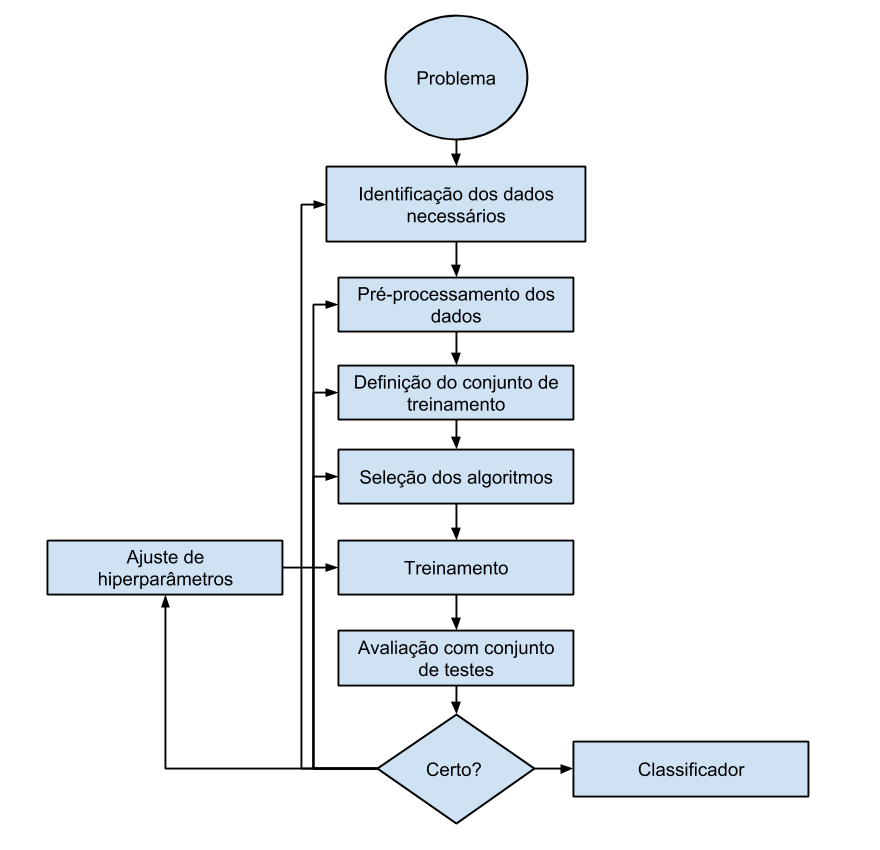
\includegraphics[width=0.8\linewidth]{images/ml_arch_pt.png}
	\label{fig:arch_ml}
  \source{\citeauthor{kotsiantis2007supervised} (\citeyear{kotsiantis2007supervised})}
\end{figure}

\subsubsection{Árvore de Decisão}

As Árvores de Decisão podem ser utilizadas principalmente para problemas relacionados à classificação de instâncias --- quando as variáveis alvo são categóricas --- e à regressão --- quando as variáveis alvo são contínuas, além disso o algoritmo em si não tem premissas sobre os dados de entrada, ou seja, é não paramétrico. Os nós internos da árvore representam as variáveis de entrada e os nós-folha as classes (variáveis alvo ou de saída) que podem ser utilizadas para classificação. As arestas, por sua vez, determinam as conjunções utilizadas para as ligações entre os diferentes nós, formando assim os caminhos possíveis entre a raiz e os nós-folha \cite{kotsiantis2007supervised}.

O uso de uma árvore de decisão envolve o processo de construção de uma árvore de decisão binária ótima, que é conhecido como um problema NP-completo. Devido a isso, existem inúmeras heurísticas eficientes para construir árvores de decisão quase ótimas, tais como a de ganho de informação, índice de gini, redução de variância, etc \cite{kotsiantis2007supervised}. 

Algumas das vantagens da árvore de decisão estão relacionadas a fácil interpretação do aprendizado (\textit{white box}), devido ao fato de ser possível visualizar e interpretar a árvore de decisão e bom desempenho com grandes volumes de dados; dentre as desvantagens, estão o alto custo computacional para grandes quantidades de variáveis e possibilidade de sobreajuste quando a árvore atinge sua altura máxima \cite{kotsiantis2007supervised, dwivedi2016automatic}.

\subsubsection{Floresta Aleatória}

Florestas aleatórias ou florestas de decisão aleatórias são um método de aprendizado conjunto (\textit{ensemble}) utilizados principalmente  para classificação e regressão. O conceito geral de classificação em conjunto é o de combinar classificadores fracos, por meio de árvores de decisão, para formar um classificador com melhores métricas de desempenho. Duas abordagens comuns para a classificação em conjunto são a de \textit{boosting} e \textit{bagging}, que podem ser implementadas como árvores impulsionadas (\textit{Boosted Trees}) e florestas aleatórias (RF --- \textit{Random Forests}), respectivamente \cite{mcdonald2014steering}.

O processo que utiliza \textit{boosting} ajusta (\textit{fit}) o algoritmo a todos os dados de entrada, em seguida encontra o conjunto de pontos classificados erroneamente e ajusta outro algoritmo (escolhido por meio de voto ponderado) aos pontos classificados incorretamente. Tal processo é repetido recursivamente com conjuntos de dados menores até que o erro fique abaixo de um determinado limiar.  Por sua vez, o processo que utiliza \textit{bagging} ajusta um algoritmo selecionando aleatoriamente do conjunto de dados original vários conjuntos de instâncias para treinamento \textit{com substituição} (um elemento pode aparecer várias vezes na amostra), ajustando em seguida um algoritmo simples (escolhidos por meio de votação majoritária) a cada uma dessas amostras \cite{mcdonald2014steering, dogru2018traffic}.

Em resumo, o algoritmo de florestas aleatórias constrói um conjunto de árvores de decisão e as une para obter predições mais precisas e estáveis. Diferentemente das árvores de decisão, o algoritmo RF previne sobreajuste por meio da criação aleatória de conjuntos de dados menores, o que implica também em árvores de menor altura. Há também a possibilidade de redução de desempenho, dependendo da quantidade de árvores criadas durante o processo de aprendizado \cite{dogru2018traffic}.

\subsubsection{K-ésimo Vizinho mais Próximo} 

O algoritmo \textit{K-ésimo Vizinho mais Próximo} (k-NN ---  \textit{k-Nearest Neighbors}) é uma abordagem para classificação e regressão não-paramétrica, na  qual o processo de aprendizado é caracterizado por encontrar um grupo de $k$ amostras que estão mais próximas de amostras desconhecidas, por exemplo, com base em funções de distância. A partir dessas $k$ amostras, as classes das amostras desconhecidas são determinadas com base nas classes mais próximas de um conjunto de pontos previamente rotulados \cite{singh2016review, thanh2018comparison}. 

Devido a característica de determinar os rótulos desconhecidos com base nos $k$ mais próximos, o k-NN é considerado um método de aprendizado ``preguiçoso'' (\textit{lazy learning}), com alto custo computacional durante a fase de classificação  e baixo na fase de treinamento. Além disso, a eficiência do algoritmo depende da escolha de um bom valor para o $k$, é afetado por ruídos, variáveis irrelevantes e pelo tamanho do conjunto de dados que precisa ser revisitado \cite{singh2016review, kibanov2018adaptive}. 

\subsubsection{Máquina de Vetores de Suporte}

O algoritmo \textit{Máquina de Vetores de Suporte} (SVM --- \textit{Support Vector Machines}) é uma abordagem de aprendizado para tarefas de classificação e regressão, que funciona em torno do conceito de ``margem'' --- de cada lado de um hiperplano responsável por separar duas classes de dados. Dessa forma, o algoritmo tem como objetivo maximizar a margem entre o hiperplano de separação e as instâncias de ambos os lados \cite{kotsiantis2006machine, singh2016review}. 

Ao contrário do k-NN, a precisão e o desempenho do SVM são independentes do tamanho do conjunto de dados, mas dependentes do número de ciclos de treinamento. Sua complexidade não é afetada pelo tamanho do conjunto de dados de treinamento (o número de vetores de suporte selecionados pelo SVM é geralmente pequeno) \cite{kotsiantis2006machine, singh2016review}.

O SVM é muito utilizado em problemas de classificação de texto, que normalmente possuem altos espaços dimensionais e tem boa capacidade de generalização. No entanto, a velocidade de treinamento é menor em relação ao k-NNN e seu desempenho depende dos hiperparâmetros escolhidos \cite{kotsiantis2006machine, singh2016review}.

Dependendo do conjunto de dados, o SVM pode não conseguir localizar um hiperplano de separação devido a instâncias atribuídas incorretamente. O problema pode ser resolvido usando uma margem flexível que aceita algumas classificações erradas das instâncias de treinamento \cite{kotsiantis2006machine}.

\subsubsection{Naive Bayes}

Uma Rede Bayesiana (\nomenclature{BN}{\textit{Bayesian Network}}{BN --- \textit{Bayesian Network}}) é um modelo gráfico para relações de probabilidade entre um conjunto de variáveis. A estrutura de rede bayesiana $S$ é um grafo acíclico direcionado (\nomenclature{DAG}{\textit{Directed Acyclic Graph}}{DAG --- \textit{Directed Acyclic Graph}}) e os nós em $S$ possuem uma correspondência um-para-um com o conjunto de variáveis $X$. As arestas, por sua vez, representam as influências casuais entre as variáveis,
 quando não existem arestas entre dois nós, não significa que eles sejam completamente independentes, pois podem ser conectados através de outros nós. Tais nós podem, no entanto, tornar-se dependentes ou independentes, dependendo da evidência que é definida em outros nós. Além disso, um nó é condicionalmente independente de seus não descendentes \cite{kotsiantis2006machine}.
 
Redes Naive Bayesianas (\nomenclature{NB}{\textit{Naive Bayesian}}{NB --- \textit{Naive Bayesian}}) são redes bayesianas muito simples que são compostas de DAGs com apenas um pai (representando o nó não observado) e vários filhos (correspondentes a nós observados) com uma forte suposição de independência entre os nós descendentes no contexto de seu pai \cite{kotsiantis2006machine}.  A suposição de independência entre nós descendentes comumente está errada e, por essa razão, os classificadores bayesianos geralmente são menos precisos do que outros algoritmos de aprendizado mais sofisticados (como o de Redes Neurais). Apesar disso, há evidências de que em determinados cenários a abordagem NB possui acurácia melhor do que algoritmos do estado da arte \cite{kotsiantis2006machine}.

A principal vantagem do NB é seu curto tempo computacional para treinamento, além disso, ao contrário das Redes Neurais ou SVM, não há hiperparâmetros a serem definidos, o que o torna mais simples de ser aplicado a uma grande variedade de tarefas. Apesar disso, o NB não é aplicável quando há necessidade de se considerar interações entre as variáveis \cite{kotsiantis2006machine, singh2016review}.

\subsubsection{Redes Neurais}

O aprendizado por meio de Redes de Neurais depende de três aspectos fundamentais: dados de entrada e função de ativação do neurônio; arquitetura da rede e o peso de cada conexão. Dado que os dois primeiros aspectos são fixos, o comportamento da rede é definido pelos valores  dos pesos. A função de ativação mais simples é popularmente conhecida como perceptron \cite{kotsiantis2006machine}.

O conceito de perceptron mapeia um conjunto de entrada de $x_1$ a $x_n$ para um valor de saída $f(x)$ (0 ou 1 de acordo com um limiar determinado), considerando $w_1$ a $w_n$ como pesos; abordagem a qual pode ser usada para aprender um aproximador de função não linear para classificação ou regressão. Perceptrons somente podem classificar conjuntos de instâncias linearmente separáveis, ou seja, se uma linha reta ou plano puder ser desenhado para separar as instâncias de entrada em suas categorias corretas, as instâncias de entrada serão linearmente separáveis e o perceptron encontrará a solução. Se as instâncias não forem linearmente separáveis, o aprendizado nunca chegará a um ponto em que todas as instâncias sejam classificadas corretamente, nesse contexto, Redes Neurais Artificiais \nomenclature{ANN}{\textit{Artificial Neural Networks}}(ANN --- \textit{Artificial Neural Networks}) as foram criadas para tentar resolver esse problema \cite{kotsiantis2006machine, singh2016review}. 

Dessa forma, os perceptrons podem ser utilizados para formar uma rede neural com multicamadas \nomenclature{MLP}{\textit{Multi-layer Perceptron}}(MLP --- \textit{Multi-layer Perceptron}), que consiste em um grande número de unidades (neurônios) unidos em um padrão de conexões. Unidades nessa rede são geralmente segregadas em três classes: unidades de entrada, que recebem informações a serem processadas; unidades de saída, onde os resultados do processamento são encontrados; e unidades centrais conhecidas como unidades ocultas. \textit{Feed-forward} ANN, como a MLP, permitem que os sinais percorram somente um caminho, da entrada à saída  \cite{kotsiantis2006machine}.

Geralmente, determinar corretamente o tamanho da camada oculta é um problema porque uma subestimativa do número de neurônios pode levar a capacidades de aproximação e generalização ruins, enquanto nós excessivos podem resultar em superajuste e eventualmente tornar a busca pelo ótimo global mais difícil  \cite{kotsiantis2006machine}.

A ANN depende de três aspectos fundamentais, funções de entrada e ativação da unidade, arquitetura de rede e o peso de cada conexão de entrada. Dentre os inúmeros  algoritmos com os quais uma rede pode ser treinada, o algoritmo de aprendizado mais conhecido e amplamente utilizado para estimar os valores dos pesos é o algoritmo \nomenclature{BP}{\textit{Back Propagation }}(BP --- \textit{Back Propagation}). No entanto, o BP tende a ser mais lento de treinar do que outros, o que pode ser problemático em redes muito grandes e com uma alta quantidade de dados. Além disso, outra desvantagem das ANN é o fato de ser difícil entender o aprendizado obtido pela rede \cite{kotsiantis2006machine, singh2016review}.

\subsubsection{Regressão Logística}

A Regressão Logística  \nomenclature{LR}{\textit{Logistic Regression}}(LR --- \textit{Logistic Regression}) é um método estatístico no qual uma curva logística é ajustada ao conjunto de dados, com o objetivo de predizer presença ou ausência de determinada característica. A LR é semelhante a um modelo de regressão linear, mas é mais adequada para modelos em que a variável dependente é dicotômica, apesar disso, essa metodologia também pode ser utilizada para predições de múltiplas classes \cite{schein2007active, kurt2008comparing, singh2016review}. 

Como a LR retorna a probabilidade de uma variável pertencer a determinada classe, os limites de classificação podem ser facilmente ajustados, no entanto, requer um tamanho de amostra grande para alcançar resultados estáveis, além de não lidar adequadamente com problemas não-lineares \cite{khemphila2010comparing, singh2016review}.

\subsection{Validação dos modelos de aprendizado supervisionado}
\label{modelValidation}

A validação dos modelos para tarefas de classificação pode ser realizada por meio de \textit{validação cruzada}\footnote{\url{https://scikit-learn.org/stable/modules/cross\_validation.html\#cross-validation}} (nos experimentos desse trabalho utilizamos 10 \textit{folds} --- subconjuntos do conjunto de dados de treinamento --- para validar a generalização dos modelos) e métricas tais como: \textit{acurácia} \nomenclature{ACC}{\textit{Accuracy}}{(ACC --- \textit{Accuracy}, Eq.~\ref{acc}), \textit{precisão} \nomenclature{PPV}{\textit{Positive Predictive Value}}{PPV --- \textit{Positive Predictive Value}, Eq.~\ref{prec})}, \textit{revocação} \nomenclature{TPR}{\textit{\textit{True Positive Rate}}}{(TPR --- \textit{True Positive Rate}, Eq.~\ref{rec}) e $f_1 score$ (Eq.~\ref{f1}), que tem como entrada o número de casos reais positivos (P), negativos (N), verdadeiro positivo (VP), verdadeiro negativo (VN), falso positivo (FP) e falso negativo (FN):

\begin{equation}
\label{acc}
ACC = \frac{VP + VN}{P + N} = \frac{TP + TN}{TP + TN + FP + FN}
\end{equation}

\begin{equation}
\label{prec}
PPV = \frac{VP}{VP + FP}
\end{equation}

\begin{equation}
\label{rec}
TPR = \frac{VP}{P} = \frac{VP}{VP + FN}
\end{equation}

\begin{equation}
\label{f1}
f_1 score = \frac{PPV * TPR}{PPV + TPR} = \frac{2VP}{2VP + FP + FN}
\end{equation}

\section{Term frequency–Inverse document frequency}

Além dos processos de NLP para redução do espaço de \textit{features} mencionados anteriormente, podemos utilizar abordagens, como a TF-IDF, que levam em consideração a frequência dos termos (\textit{tokens}) existentes em um conjunto de documentos. TF-IDF é um algoritmo de ponderação de variáveis que combina as ponderações \emph{frequência do termo} \nomenclature{TF}{\textit{Term Frequency}}{(TF --- \textit{Term Frequency})} e \emph{inverso da frequência nos documentos} (\nomenclature{IDF}{Inverse Document Frequency}{IDF --- \textit{Inverse Document Frequency}}) para calcular os pesos dos termos linguísticos (variáveis) em um determinado corpus. Em outras palavras, o peso da variável é proporcional a frequência com a qual aparece nos documentos, e inversamente proporcional a quantidade de documentos que contém o termo linguístico em questão \cite{wu2018improved, yahav2018comments}. 

Dentre as variações de implementação da ponderação $W_{t,d}$ (TF-IDF) existentes, a abordagem tradicional considera uma coleção de termos $t \in T$ que aparecem em um conjunto de N documentos $d \in D$, posto isso, defini-se como o produto entre $tf_{i,j}$ e $idf_i$ --- onde $n_{i,j}$ é a frequência do termo $t_i$ no documento $d_j$, $\sum_k n_{k,j}$ o somatório da frequência de todos os termos do documento $d_j$ e $n$ o número de documentos onde $t_i$ aparece ($n + 1$, caso $n = 0$) --- conforme a s seguinte equações \cite{wu2018improved}:

\begin{equation}
tf_{i,j} = \frac{n_{i,j}}{\sum_k n_{k,j}}
\end{equation}
\begin{equation}
idf_i = \log \frac{N}{n + 1}
\end{equation}
\begin{equation}
W_{t,d} = tf_{t,d} * idf_t
\end{equation}

No contexto deste trabalho, entendemos documentos como as classes dos eventos de exceção. A \emph{frequência dos termos} (TF --- $tf_{t,d}$) é determinada por classe e a \emph{frequência do termo - inverso da frequência nos documentos} (IDF --- $idf_t $) como o inverso dos eventos de exceção, sendo $N$ o tamanho do conjunto dos eventos de exceção, sob o qual $df_t$ é definido. Os eventos de exceção são classificados em suas respectivas classes por meio dos modelos de aprendizado supervisionado, elencados na Seção~\ref{supervisionedLearning}. 

\section{Algoritmo \textit{Apriori}}
\label{apriori}

O algoritmo \textit{Apriori}\footnote{Utilizamos para este trabalho a implementação do algoritmo \textit{Apriori} feita pela biblioteca \textit{Apyori}  \url{https://pypi.org/project/apyori}}. Acesso em 08 de janeiro de 2019} normalmente é utilizado em mineração de texto para identificar relações entre conjuntos de itens e padrões, por meio de comparações de conjuntos de itens frequentes, para assim determinar regras de associação com base em métricas, tais como a de \textit{suporte} (\textit{support}) --- indicador da frequência de determinados registros no conjunto de dados; \textit{confiança} (\textit{confidence}) --- frequência com que determinadas regras de associações entre registros são encontradas como verdadeiras e \textit{lift} --- probabilidade de ocorrência de um consequente B no conjunto de dados ($lift > 1$ indica que a regra de associação em questão pode ser utilizada para predição de um consequente B em conjuntos de dados futuros). É importante observar que a notação $A \rightarrow B$ se refere a antecedente e consequente, respectivamente. Todas as métricas mencionadas anteriormente são detalhadas nas equações~\ref{eqSupportA},~\ref{eqSupportB},~\ref{eqSupports},~\ref{eqConfidence} e~\ref{eqLift} a seguir  \cite{park2018apriori}:

\begin{equation}
\label{eqSupportA}
support(A) = \dfrac{\sum_{i=1}^{n}[A \in s_i]} {n} = P(A) 
\end{equation}

\begin{equation}
\label{eqSupportB}
support(B) = \dfrac{\sum_{i=1}^{n}[B \in s_i]} {n} = P(B) 
\end{equation}

\begin{equation}
\label{eqSupports}
support(A \rightarrow B) = \dfrac{\sum_{i=1}^{n}[A \in s_i \land B \in s_i]} {n} = P(A \cap B)
\end{equation}

\begin{equation}
\label{eqConfidence}
confidence(A \rightarrow B) = \dfrac{support(A \rightarrow B)}{support(A)} = \dfrac{P(A \cap B)}{P(A)} = P(B|A)
\end{equation}

\begin{equation}
\label{eqLift}
lift(A \rightarrow B) = \dfrac{confidence(A \rightarrow B)}{support(B)} = \dfrac{P(B|A)}{P(B)}
\end{equation}

Algoritmos para mineração de dados, como o \textit{Apriori}, não tem tido seu potencial explorado no domínio de grandes volumes de dados relacionados ao transporte \cite{park2018apriori}. Neste trabalho, aplicamos o algoritmo \textit{Apriori} no conjunto de dados da \textit{SPTrans} para identificarmos as regras de associação existentes, detalhadas na Seção~\ref{expApriori}, com o objetivo de contribuirmos para a gestão do transporte público por ônibus da cidade de São Paulo.   

\chapter{Revisão Sistemática}
\label{revisao}
Conforme mencionado na Seção \ref{objetivos} o objetivo geral desse projeto de pesquisa é a caracterização de eventos de exceção e de seus respectivos impactos no sistema de transporte público por ônibus da cidade de São Paulo, por meio do cruzamento de dados AVL, da GTFS e \textit{tweets} das contas oficiais responsáveis por reportar esse tipo de evento. Devido a isso este capítulo apresenta uma \nomenclature{RS}{Revisão Sistemática}{Revisão Sistemática (RS)} com o objetivo de encontrar o estado da arte de trabalhos que visam melhorar sistemas de transporte público por meio do processamento de \textit{tweets} em conjunto com outras fontes de dados.

Além disso, de uma forma mais ampla, busca-se também entender como os \textit{tweets} têm sido utilizados na caracterização de problemas urbanos. Sendo assim, o capítulo é iniciado com a seção sobre o planejamento da Revisão Sistemática; seguida das questões de pesquisa utilizadas na formulação do problema da RS; do processo de coleta dos estudos primários; da avaliação dos dados coletados; da análise e interpretação dos estudos selecionados, concluindo com as considerações finais.

% \begin{CCSXML}
% <ccs2012>
% <concept>
% <concept_id>10003120.10003130.10003134.10003293</concept_id>
% <concept_desc>Human-centered computing~Social network analysis</concept_desc>
% <concept_significance>500</concept_significance>
% </concept>
% <concept>
% <concept_id>10011007.10011074.10011081.10011082.10011083</concept_id>
% <concept_desc>Software and its engineering~Agile software development</concept_desc>
% <concept_significance>500</concept_significance>
% </concept>
% </ccs2012>
% \end{CCSXML}

% \ccsdesc[500]{Human-centered computing~Social network analysis}
% \ccsdesc[500]{Software and its engineering~Agile software development}

\section{Planejamento da Revisão Sistemática}
\label{planejamento}
A presente Revisão Sistemática utiliza a metodologia proposta por \citeauthor{biolchini2005techincal} (\citeyear{biolchini2005techincal}), composta por cinco etapas.
A primeira etapa está relacionada à formulação do problema, na qual é levantada uma questão central se referindo ao tipo de evidência que deverá  estar contida na revisão. Em seguida, são construídas definições que permitem estabelecer uma distinção entre os estudos relevantes e irrelevantes para o propósito específico do que se está investigando \cite{biolchini2005techincal}.

A segunda etapa da condução está relacionada à Coleta de Dados, na qual são definidos os procedimentos que serão utilizados para encontrar a evidência relevante que foi definida na etapa anterior. Nesta fase é extremamente importante determinar as fontes que podem fornecer estudos relevantes a serem incluídos na pesquisa \cite{biolchini2005techincal}.

Na terceira etapa a Avaliação de Dados é definida, na qual são selecionadas as fontes primárias que deverão ser incluídas na revisão. Em seguida,  são aplicados os critérios de qualidade para separar estudos que podem ser considerados válidos, e determinadas as diretrizes para o tipo de informação que deve ser extraída dos relatórios de pesquisas primárias \cite{biolchini2005techincal}.

A quarta etapa da revisão é o processo de Análise e Interpretação, na qual os dados dos estudos primários válidos são sintetizados. E, na quinta etapa são realizados os processos de Conclusão e Apresentação \cite{biolchini2005techincal}.

\subsection{Justificativa da Revisão Sistemática}
\label{justificativa}
Esta Revisão Sistemática se justifica por não terem sido encontradas revisões sistemáticas com o foco em questões urbanas e de transporte público, abordando unicamente o processamento de \textit{tweets}. Em \cite{Chaniotakis2016}, por exemplo, foi realizado um mapeamento de forma não sistemática dos trabalhos sobre o uso das mídias sociais em problemas relacionados ao transporte público; \cite{steiger2015advanced}, por outro lado, desenvolveram uma revisão sistemática sobre o uso do \textit{Twitter} para questões espaço-temporais; e \cite{jungherr2016twitter} no contexto político.%

Devido a isso, a presente revisão sistemática se diferencia por ter como objetivo encontrar o estado da arte de trabalhos que visam melhorar sistemas de transporte público por meio do processamento de \textit{tweets}, cruzando-os com outras fontes de dados. Além disso, de uma forma mais ampla, busca-se também entender como os \textit{tweets} têm sido utilizados na caracterização  de problemas urbanos.

\section{Questões de Pesquisa}
\label{questoes}
Nesta seção, são apresentadas as questões de pesquisa utilizadas para a formulação dos problemas abordados por essa Revisão Sistemática. Por meio das quais, busca-se atender os objetivos já mencionados na Seção~\ref{justificativa}.

\begin{enumerate}

\item Quais os tipos de problemas urbanos abordados utilizando processamentos de \textit{tweets}?
\label{item:1} \newline \newline
O propósito da \nomenclature{QP}{Questão de Pesquisa}{QP1} é identificar quais são as contribuições do processamento de \textit{tweets} para a mitigação de problemas urbanos. A resposta a essa questão de pesquisa ajudará especialistas das áreas multidisciplinares relacionadas ao Urbanismo (como a de Análise de Redes Sociais e Políticas Públicas) a terem um panorama de como \textit{tweets} podem ser utilizados para ajudar na solução de problemas urbanos. \newline

Uma análise preliminar dos estudos primários permite elaborar a seguinte \nomenclature{HP}{Hipótese de Pesquisa}{Hipótese de Pesquisa (HP1):} alguns dos problemas urbanos abordados estão relacionados ao transporte, mobilidade urbana, turismo e desastres naturais. \newline

\item Como \textit{tweets} têm sido utilizados para abordar problemas relacionados ao transporte público? \newline \newline
\label{item:2}
O propósito da QP2 é identificar se \textit{tweets} têm sido utilizados para solucionar problemas relacionados ao transporte público. A resposta a essa questão de pesquisa ajudará especialistas das áreas multidisciplinares relacionadas ao Urbanismo (como a de Análise de Redes Sociais e Políticas Públicas) a terem um panorama de como \textit{tweets} podem ser utilizados para ajudar na solução de problemas referentes a mobilidade urbana. \newline

Uma análise preliminar dos estudos primários permite elaborar a seguinte Hipótese de Pesquisa (HP2): \textit{tweets} têm sido utilizados principalmente para questões relacionadas ao congestionamento, não tendo como foco o transporte público.\newline

\item Quais as técnicas estatísticas utilizadas no processamento de \textit{tweets}?
\label{item:3} \newline \newline
O propósito da QP3 é identificar quais as técnicas estatísticas utilizadas no processamento de \textit{tweets}, principalmente no que se refere a validação do processo de aprendizado. A resposta a essa questão de pesquisa ajudará especialistas a terem um panorama de como validar tarefas de aprendizado que utilizam dados oriundos de \textit{tweets}. \newline

Uma análise preliminar dos estudos primários permite elaborar a seguinte Hipótese de Pesquisa (HP3): \textit{${F_1}$ score} é a principal técnica utilizada para validação de classificação binária.\newline

\item Quais os paradigmas de processamento têm sido utilizados ao lidar com \textit{tweets}?
\label{item:4} \newline \newline
O propósito da QP4 é identificar os paradigmas utilizados para processamento de \textit{tweets}. A resposta a essa questão de pesquisa ajudará especialistas a terem um panorama das técnicas de processamento utilizadas na análise de \textit{tweets}. \newline

Uma análise preliminar dos estudos primários permite elaborar a seguinte Hipótese de Pesquisa (HP4): o principal paradigma utilizado tem sido o processamento de \textit{tweets} em lote (\textit{batch} --- \textit{offline}), após um processo de armazenamento. Poucos são os estudos que constroem uma plataforma para processamento de dados em tempo real. \newline

\item Quais são os eventos de exceção relacionados ao transporte público?
\label{item:5} \newline \newline
O propósito da QP5 é identificar os eventos de exceção relacionados ao transporte público. A resposta a essa questão de pesquisa ajudará especialistas no levantamento de eventos de exceção relacionados ao transporte público, os quais podem ser utilizados em algoritmos de classificação.\newline

Uma análise preliminar dos estudos primários permite elaborar a seguinte Hipótese de Pesquisa (HP5): há poucos ou nenhum estudo que, ao tratar de problemáticas relacionadas ao transporte público, realizam um levantamento dos eventos de exceção desse contexto.\newline

\item Quais as técnicas de aprendizado de máquina utilizadas no processamento de \textit{tweets}?
\label{item:6} \newline \newline
O propósito da QP6 é identificar as técnicas de aprendizado de máquina utilizadas no processamento de \textit{tweets}. A resposta a essa questão de pesquisa ajudará especialistas a terem um panorama das principais técnicas de aprendizado de máquina utilizadas no processamento de \textit{tweets}. \newline

Uma análise preliminar dos estudos primários permite elaborar a seguinte Hipótese de Pesquisa (HP6): a técnica \textit{Support Vector Machine} tem sido utilizada na maioria dos estudos que aplicam aos \textit{tweets} algum algoritmo de aprendizado de máquina.\newline
\end{enumerate}

\section{Coleta de dados}
\label{coleta}
Nesta Revisão Sistemática, os artigos foram coletados em quatro fontes de pesquisa, por meio da plataforma de indexação de trabalhos acadêmicos \textit{Google Scholar}\footnote{\url{https://scholar.google.com}. Acesso em 29 de outubro de 2017.}. Constam na Tabela~\ref{tab:tableNumberOfArticles} as bases pesquisadas no ano de 2017, quantidades de artigos coletados, descartados no processo de filtragem (Figura~\ref{fig:filter}, descrito na Seção~\ref{avaliacao}) e selecionados. Com base na QP1, a seguinte \textit{string} de busca foi construída; restrita aos trabalhos publicados entre 2011 e 2016, escritos no idioma Inglês (devido ao fato das publicações relevantes, na área de Computação, estarem disponíveis nesse idioma): \newline

\textbf{\textit{String} de busca:} twitter urban planning city (analytics OR patterns OR tweets OR social OR media) AND (public transport) \newline

\textbf{Palavras-chave:} twitter, urban, planning, city, analytics, patterns, tweets, social, media e public transport.

\begin{table}[!htb]
\centering
\caption{Quantidades de artigos coletados e fontes de busca}
	\label{tab:tableNumberOfArticles}
\begin{tabular}{c|c|c|c}
\toprule
\textbf{Fonte} & \textbf {Artigos coletados} & \textbf{Filtragem} & \textbf{Selecionados}\\ 
\midrule
\nomenclature{ACM}{\textit{Association for Computing Machinery}}{ACM} & 44 & 34 & 10 \\ 
\hline
\nomenclature{IEEE}{\textit{Institute of Electrical and Electronics Engineers}}{IEEE} & 82 & 74 & 8 \\ 
\hline
Elsevier & 81 & 72 & 9\\ 
\hline
Springer & 22 & 20 & 2\\ 
\midrule
\midrule
\textbf{Total} & 229 & 200 & 29\\ 
\bottomrule
\end{tabular}
\source{Felipe Cordeiro Alves Dias (2019)}
\end{table}

\begin{figure}[H]% H manda colocar exatamente nessa posição no texto (relativa aos parágrafos anterior e posterior)
	\centering
 	  \caption{Processo de Filtragem}
		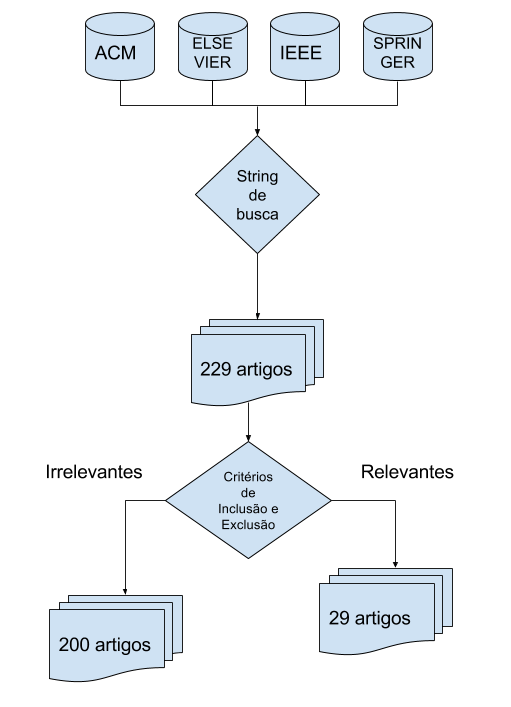
\includegraphics[width=0.5\linewidth]{images/metodologia_metodologia.png}
	\label{fig:filter}
  \source{Felipe Cordeiro Alves Dias (2019)}
\end{figure}

\section{Avaliação de Dados}
\label{avaliacao}

Visando selecionar os artigos relevantes para esta Revisão Sistemática, os seguintes critérios foram utilizados no processo de filtragem:

\begin{itemize}
\item Trabalho publicado (critério de qualidade).
\item Trabalhos que utilizam \textit{tweets} para abordar questões urbanas e de transporte público.
\item Trabalhos duplicados.
\item Trabalhos que estão fora do escopo da questão de pesquisa.
\end{itemize}

O processo de condução da Revisão Sistemática foi realizado utilizando os critérios acima mencionados. Após o processo de condução, alguns dos metadados dos artigos selecionados foram sintetizados. Sendo assim, a Figura~\ref{fig:w_cloud} apresenta uma nuvem de \textit{tags} (gerada com a biblioteca \textit{wordcloud} \cite{wordcloud}) sintetizando as palavras chaves dos estudos primários selecionados; e a Figura~\ref{fig:qtd} a quantidade de artigos publicados por ano, sendo possível analisar por meio dela a distribuição dos artigos entre 2011 e 2016, assim como sua respectiva porcentagem, ilustrada na Figura~\ref{fig:porcentagem}.

\begin{figure}[H]% H manda colocar exatamente nessa posição no texto (relativa aos parágrafos anterior e posterior)
	\centering
 	  \caption{Quantidade de artigos publicados por ano}
		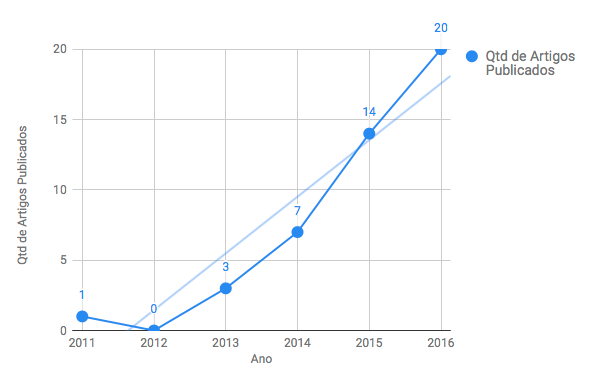
\includegraphics[width=0.8\linewidth]{images/g1.png}
	\label{fig:qtd}
  \source{Felipe Cordeiro Alves Dias (2019)}
\end{figure}

\begin{figure}[H]% H manda colocar exatamente nessa posição no texto (relativa aos parágrafos anterior e posterior)
	\centering
 	  \caption{Porcentagem dos artigos publicados por ano}
		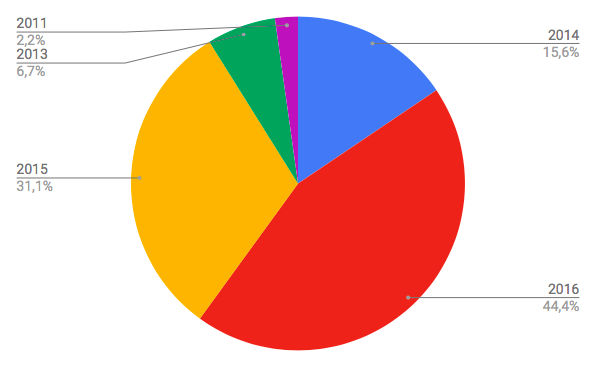
\includegraphics[width=0.8\linewidth]{images/g2.png}
	\label{fig:porcentagem}
  \source{Felipe Cordeiro Alves Dias (2019)}
\end{figure}

\begin{figure}[H]% H manda colocar exatamente nessa posição no texto (relativa aos parágrafos anterior e posterior)
	\centering
 	  \caption{Nuvem de palavras das palavras chaves dos artigos selecionados}
		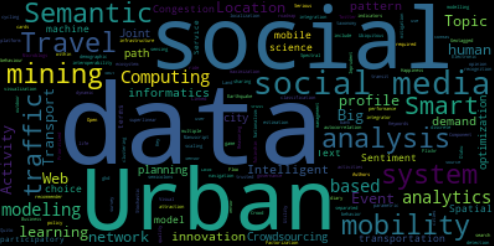
\includegraphics[width=0.8\linewidth]{images/world_cloud_metodologia.png}
	\label{fig:w_cloud}
  \source{Felipe Cordeiro Alves Dias (2019)}
\end{figure}

\section{Análise e Interpretação}
\label{analise}
Nesta seção é realizada a análise e interpretação dos estudos primários selecionados pela Revisão Sistemática, sendo as seções divididas de acordo com as questões de pesquisa.
\subsection{Tipos de problemas urbanos abordados utilizando o processamento \textit{tweets} (QP1)}

Os tipos de problemas urbanos abordados utilizando o processamento de \textit{tweets} foram divididos nas seguintes categorias: 

\begin{enumerate}
\item \textit{\textbf{e-Participation}} (interação entre  cidadãos  e órgãos civis) \cite{Mukherjee2015, Soomro2016};
\item \textbf{detecção de zoneamento urbano} \cite{Frias-Martinez2014};
\item \textbf{identificação de pontos de interesse} \cite{Farseev2015, Gutev2016, Bendler2014, Abbasi2015, Gkiotsalitis2015, Gkiotsalitis2016, Hasan2014, Maghrebi2015, DiLorenzo2013};
\item \textbf{mobilidade} \cite{Gutev2016, Chen2016, Yousaf2014};
\item \textbf{padrões demográficos} \cite{Farseev2015, Gutev2016, Steiger2015Census, Guo2016};
\item \textbf{poluição} \cite{Zagal2016};
\item \textbf{segurança pública} \cite{Wen2016, Mata2015};
\item \textbf{turismo} \cite{Thomaz2016, Abbasi2015, Chua2016, Sobolevsky2015};
\item \textbf{tráfego} \cite{Anantharam2015, Lecue2014}.
\end{enumerate}

Conforme os estudos primários analisados pela Revisão Sistemática, e enumerados nessa seção, é possível interpretar que \textit{tweets} podem ser utilizados para auxiliar na mitigação de inúmeros problemas urbanos. Apesar disso, em \cite{Chaniotakis2015} os autores observam que os \textit{tweets} contendo informações sobre geolocalização são normalmente publicados em áreas relacionadas ao lazer, além de haver correlação entre regiões urbanas com maior renda \textit{per capita} e o número de \textit{tweets} postados. Tal evidência pode conduzir viés nas análises por representar somente algumas classes econômicas da população. 

Considerando a observação anterior, um dos estudos analisados foi o realizado por \cite{Zagal2016}, na Cidade do México. Nesse estudo, foram mapeados os pontos da cidade referenciados em publicações relacionadas a doenças respiratórias e poluição, orientando tomadas de decisão no aspecto ambiental. 

Além disso, há também exemplos de trabalhos relacionados a Segurança Pública, como o estudo de caso realizado por \cite{Wen2016}, no qual foi enriquecido um conjunto de dados com \textit{tweets} geolocalizados, visando analisar o impacto dos ataques terroristas (em Paris, em novembro de 2015) nos padrões de atividades urbanas (relacionadas ao uso de transporte público, serviços, realização de compras, e atividade noturna). Em um outro caso de aplicação, estimou-se por meio de \textit{tweets}, a probabilidade de ocorrência de crimes e ameaças nas ruas da Cidade do México, sugerindo rotas seguras aos pedestres \cite{Mata2015}.

Também, foram encontrados na literatura estudos que utilizaram \textit{tweets} para inferir padrões demográficos. Por exemplo, em \cite{Farseev2015, Gkiotsalitis2015, Gkiotsalitis2016}, os autores processaram \textit{tweets} para analisar a distribuição etária e de gênero da população, assim como seus respectivos pontos de interesse (como locais para entretenimento, residência, trabalho, recriação, compras, educação e serviços sociais) \cite{Hasan2014, Maghrebi2015}. 

Tais pontos de interesse podem ser utilizados em problemas relacionados ao transporte público \cite{Gutev2016} e também ao turismo, como no estudo realizado por \cite{Abbasi2015} para identificar a locomoção de visitantes e residentes em pontos turísticos de Sydney; por \cite{Chua2016}, ao caracterizar aspectos espaciais, temporais e demográficos, dos turistas da cidade de Cilento, Itália; e por \cite{Thomaz2016} na cidade de Curitiba (Brasil), no contexto da Copa do Mundo de 2014.

Nesse mesmo contexto, \cite{Guo2016} estudaram algumas questões demográficas por meio de análise de sentimento e encontraram correlação positiva entre oportunidades de emprego e sentimentos positivos, e negativa entre felicidade e número de crianças na população da Grande Londres. Outro caso de uso, foi o desenvolvido em \cite{Steiger2015Census}, no qual os autores usaram \textit{tweets} para identificar diferentes tipos de atividades em Londres, correlacionadas com informações censitárias; e em \cite{Sobolevsky2015} ao estudar a atratividade da Espanha a turistas.

Um dos problemas relacionados à identificação de pontos de interesse se refere as incertezas espaço-temporais e de determinação de tópicos, o qual foi abordado pelo trabalho realizado por \cite{Bendler2014}. Nele, os autores contribuíram com uma técnica para minimizar o problema ao processar \textit{tweets}; analisando a causalidade entre o tempo e local das postagens realizadas, reduzindo assim os índices de incerteza, no contexto da cidade de São Francisco, EUA. Outro problema, relaciona-se com a questão da privacidade, pois as localizações dos usuários podem ser inferidas mesmo quando não disponibilizadas. Nesse cenário, \cite{Wang2017} propõem um \nomenclature{PTCS}{Sistema de Calibração de Trajetórias Privadas}{Sistema de Calibração de Trajetórias Privadas (PTCS),} por meio de mecanismos de Privacidade Diferencial e de \textit{k-anonymity}, com isso é possível extrair informações sobre trajetórias sem exposição de informações sensíveis, testado na extração de localizações contidas em \textit{tweets}. 

Outro contexto na literatura revisada está relacionado ao processamento dos eventos que acontecem na cidade (idealmente em tempo real, como sugerem \cite{Soomro2016}). Um dos estudos encontrados sobre esse assunto, foi o realizado por \cite{Anantharam2015}, no qual os autores desenvolveram uma técnica para identificar os diferentes tipos de eventos do cotidiano urbano, rotulando-os sequencialmente, por meio da anotação de \textit{tweets} e extração de eventos, considerando aspectos espaciais, temporais e temáticos. Para isso, utilizaram-se dos conhecimentos de domínio, tais como informações sobre os locais em uma cidade e possíveis termos para os eventos, identificando assim os relacionados ao tráfego da região da Baia de São Francisco, EUA. 

Sobre a mesma temática, \cite{DiLorenzo2013} desenvolveram uma ferramenta inteligente e interativa para exploração visual da dinâmica de eventos sociais ao longo das dimensões espacial, temporal e organizacional. O tráfego também foi objeto de estudo em \cite{Chen2016}, ao relacionar eventos do trânsito com a demanda por bicicletas; e em \cite{Lecue2014}, ao demonstrar uma plataforma para análise inteligente do tráfego (em tempo real), com base em fontes heterogêneas de dados (incluindo \textit{tweets} de agências oficiais de trânsito).

Em uma abordagem mais genérica, \cite{Mukherjee2015} propuseram uma plataforma para processar (em \textit{near real time}) questões urgentes da cidade, oriundas de diversas fontes (incluindo o \textit{Twitter}), atuando como intermediadora entre cidadãos e agências civis. No que se refere a mobilidade urbana, mas não ao uso de informações sobre pontos de interesse, \cite{Yousaf2014} inferiram a afinidade entre usuários por meio da análise de \textit{retweets}, possibilitando que rotas de corridas sejam compartilhadas entre pessoas com interesses em comum, tornando a viagem mais agradável.

Por fim, em \cite{Frias-Martinez2014}, os autores utilizaram apenas \textit{tweets} geolocalizados para analisar suas respectivas distribuições no espaço urbano, com o objetivo de identificar a caracterização do uso da terra em zoneamentos urbanos industriais, residenciais, comerciais e de lazer. O trabalho foi realizado no contexto da cidade de Manhattan (EUA), Londres (Reino Unido) e Madrid (Espanha).

\subsection{Casos de uso relacionados ao transporte público (QP2)}
Nesta seção, são identificados os estudos primários que utilizam processamento de \textit{tweets} com foco na mitigação dos problemas relacionados ao transporte público; enumerados a seguir:
\begin{enumerate}
\item \textbf{Impacto de eventos no transporte público}:
\begin{enumerate}
\item impacto dos ataques terroristas em Paris no uso do transporte público \cite{Wen2016};
\item impacto de eventos relacionados ao tráfego na demanda por bicicletas, em Nova Iorque e Washington D.C, EUA \cite{Chen2016};
\item impacto dos pontos de interesse na demanda por transporte público \cite{Maghrebi2015};
\item impacto dos eventos anormais nas tomadas de decisão dos passageiros do Metrô de Tóquio \cite{Itoh2016};
\item predição de fluxo de passageiros no Metrô de Nova Iorque \cite{Ni2016}.
\end{enumerate}

\item \textbf{Planejamento e gestão do transporte público}:
\begin{enumerate}
\item análise de sentimento relacionada ao acesso ao transporte público \cite{Guo2016};
\item coleta de informações relacionadas ao transporte público \cite{Gal-Tzur2014};
\item identificação de locais para estações de bicicletas, em St. Petersburg, Rússia \cite{Gutev2016};
\item identificação da disposição dos usuários para realizar viagens de lazer \cite{Gkiotsalitis2016};
\item plataforma para notificação de problemas relacionados ao transporte público de Bangalore, Índia \cite{Mukherjee2015}.
\end{enumerate} 
\end{enumerate}

Conforme os estudos primários analisados pela Revisão Sistemática, e enumerados nessa seção, é possível interpretar que os estudos estão classificados em análise de impacto de eventos, planejamento e gestão do transporte público. Por exemplo, \cite{Wen2016} utilizaram \textit{tweets} para analisar o impacto dos ataques terroristas em Paris (2015) nos padrões de mobilidade referentes ao uso de transporte público. Semelhantemente, \citeauthor{Itoh2016} (\citeyear{Itoh2016}) desenvolveram uma ferramenta para analisar e explorar visualmente, com base em \textit{tweets}, as tomadas de decisão dos passageiros do Metrô de Tóquio, ante a eventos anormais, tais como Tufões, Incêndios, Terremotos, dentre outros. Nesse mesmo contexto, \cite{Ni2016} propuseram uma técnica de predição de fluxo de passageiros no Metrô de Nova Iorque, identificando eventos com base nas \textit{hashtags} dos \textit{tweets}. Enquanto que em \cite{Chen2016}, analisaram a relação entre eventos do tráfego com a demanda por bicicletas.

No que se refere aos estudos focados no planejamento e gestão do transporte público, \cite{Mukherjee2015} apresentam uma plataforma desenvolvida e utilizada pela Agência de Transporte Público de Bangalore, na Índia, a qual permite que usuários reportem questões relacionadas ao transporte  público, o que possibilita a melhoria do planejamento de suas respectivas operações, assim como do serviço prestado para a população. Nessa mesma linha de estudo, em \cite{Gutev2016}, os autores usaram \textit{tweets} para identificar a popularidade de determinados locais, pontos de interesse e distribuição etária, com o objetivo de determinar os melhores pontos para estações de bicicletas e incentivar assim o uso desse modal de transporte. Também relacionado aos pontos de interesse, \cite{Maghrebi2015} utilizaram \textit{tweets} para identificar padrões das atividades humanas (em diferentes horários do dia) e seus respectivos impactos na demanda por transporte público.

Em \cite{Gal-Tzur2014}, por sua vez, utilizaram uma abordagem hierárquica para classificar \textit{tweets} relacionados ao transporte. Com isso, demonstraram que é possível usar essas informações para fins de planejamento e gerenciamento do transporte. Tal técnica, foi aplicada em um estudo de caso associado a eventos esportivos, ocorridos no Reino Unido. A hierarquia é composta por três níveis, no primeiro, os \textit{tweets} são classificados entre os que expressam a necessidade de serviços de transporte, opiniões e incidentes; o segundo, identifica a categoria do transporte; e último, relaciona \textit{tweets} a tópicos. 

Outro estudo que contribui com o planejamento do transporte público, é o realizado em (\citeauthor{Gkiotsalitis2015}, \citeyear{Gkiotsalitis2015}, \citeyear{Gkiotsalitis2016}), no qual \textit{tweets} foram processados para identificar a disposição dos usuários para realizar viagens relacionadas ao lazer (pontos de interesse), sugerindo a eles atividades com menor tempo de percurso e probabilidade de atrasos. Além do tempo de percurso, outro ponto relevante considerado foi o de bom nível de acesso ao transporte público, o qual quando existente impacta positivamente na felicidade das pessoas e se correlaciona com sentimentos positivos, segundo a análise de sentimentos realizada por \cite{Guo2016}, utilizando \textit{tweets} publicados na Grande Londres.

\subsection{Técnicas estatísticas utilizadas no processamento de \textit{tweets} (QP3)}
Nesta seção, são apresentadas as técnicas estatísticas utilizadas pelos estudos primários, no processamento de \textit{tweets}, enumeradas a seguir:

\begin{enumerate}
\item \textbf{Análise de métricas relacionadas a desempenho} (erro de reconstrução relativo, qualidade dos componentes descritivos recuperados e qualidade dos componentes comuns recuperados) \cite{Wen2016};
\item \textbf{semelhança de cosseno} (Cosine similarity) \cite{Yousaf2014, Frias-Martinez2014};
\item \textbf{\textit{\bm{${f_1}$} score}} \cite{Anantharam2015, Chen2016};
\item \textbf{frequência do termo–inverso da frequência nos documentos} (TF-IDF --- \textit{\textbf{Term frequency–inverse document frequency}} \cite{Mukherjee2015};
\item \textbf{coeficiente de variação inversa} \cite{Bendler2014};
\item \textbf{método de reamostragem Jackknife} \cite{Bendler2014};
\item \nomenclature{LISA}{\textit{Local Indicators of Spatial Association}}{\textbf{indicadores locais de associação espacial} (\textbf{LISA} --- \textit{\textbf{Local Indicators of Spatial Association}}))} \cite{Steiger2015Census};
\item \textit{\textbf{local Moran's}} \cite{Steiger2015Census};
\item \textbf{máxima verossimilhança} \cite{Mukherjee2015};
\item \nomenclature{SARIMA}{\textit{Seasonal Autoregressive Integrated Moving Average}} \textbf{média móvel integrada autoregressiva sazonal} (\textbf{SARIMA} --- {\textit{\textbf{Seasonal Autoregressive Integrated Moving Average}})} \cite{Ni2016};
\item \textbf{otimização e previsão com função de perda híbrida} \cite{Ni2016}.
\end{enumerate}
 
Em \cite{Ni2016}, os autores utilizaram a técnica SARIMA em conjunto com Regressão Linear, propondo uma abordagem baseada em otimização paramétrica e convexa, chamada \textit{otimização e previsão com função de perda híbrida}, adequada para modelagem utilizando séries temporais. Com isso, tal técnica foi aplicada na predição de fluxo de passageiros com base em \textit{hashtags} de \textit{tweets}.  

Referente aos problemas relacionados a ambiguidade e identificação de contextos, \cite{Anantharam2015}; \cite{Chen2016, Gal-Tzur2014} aplicaram a técnica \textit{${F_1}$ score} validar o processo de classificação de \textit{tweets}. Por outro lado, \cite{Mukherjee2015} utilizaram a técnica de \textit{máxima verossimilhança} para determinar a probabilidade de ocorrência de um evento, assim como a confiabilidade da informação.

No que se refere a agrupamento, \cite{Yousaf2014} agruparam usuários por meio de \textit{semelhança de cossenos}, unindo pessoas com interesses em comum nos mesmos grupos. \cite{Frias-Martinez2014}, por outro lado, usou a mesma técnica para agrupar \textit{tweets} de acordo com suas semelhanças quanto aos tipos de zoneamento urbano.

De forma isolada, no trabalho realizado por \cite{Mukherjee2015}, utilizaram a técnica TF-IDF na fase de classificação para o definir o \textit{score} de categorias de eventos, escolhendo a mais relevante a ser buscada em um dicionário de categorias. Também isoladamente, \cite{Steiger2015Census} usaram a técnica LISA na identificação de \textit{clusters} espaciais e valores esporádicos espaciais, obtendo assim os locais com atividades sociais. Além disso, os autores também utilizaram a técnica \textit{Local Moran's} para detectar diferentes padrões de atividade de acordo com o espaço geográfico.

Por último, \cite{Bendler2014} inovaram ao utilizar o \textit{método de reamostragem Jackknife} como inspiração para o desenvolvimento de uma abordagem que visa analisar a estabilidade estatística de um conjunto de categorias. Além disso, usaram também a análise do \textit{coeficiente de variação inversa} para verificar a dispersão negativa da distribuição de um conjunto de variáveis. 

\subsection{Paradigmas de processamento (QP4)}
Nesta seção, encontram-se a seguir apenas os paradigmas de processamento extraídos dos estudos primários analisados: 
\begin{enumerate}
\item \textbf{Processamento em lote} (\textit{\textbf{batch, offline processing}}) \cite{Anantharam2015, Wen2016, Farseev2015, Gutev2016, Mata2015, Chen2016, Abbasi2015, Bendler2014, Yousaf2014, Frias-Martinez2014, Steiger2015Census, Gal-Tzur2014, Gkiotsalitis2016, DiLorenzo2013, Itoh2016, Chaniotakis2015};
\item \textbf{processamento em quase tempo real} (\textit{\textbf{Near real time}}) \cite{Mukherjee2015};
\item \textbf{processamento em tempo real} (\textit{\textbf{Real time processing}}) \cite{Soomro2016, Lecue2014}.
\end{enumerate}

\subsection{Eventos de exceção relacionados ao transporte público (QP5)}
\label{qp5}

Nesta seção, encontram-se a seguir os eventos de exceção relacionados ao transporte público, extraídos dos estudos primários:

\begin{enumerate}
\item \textbf{Acidentes} \cite{Itoh2016}:
\begin{enumerate}
\item acidentes nas estações transporte;
\item incêndio.
\end{enumerate}

\item \textbf{Espaço-temporais}  \cite{Chen2016}:
\begin{enumerate}
\item dia da semana;
\item hora do dia.
\end{enumerate}

\item \textbf{Eventos sociais} \cite{Chen2016, Lecue2014, Gal-Tzur2014, Itoh2016}:
\begin{enumerate}
\item feiras de rua;
\item festivais;
\item jogos esportivos;
\item passeatas e maratonas.
\end{enumerate}

\item \textbf{Eventos urbanos} \cite{Chen2016, Lecue2014}:
\begin{enumerate}
\item relacionados ao tráfego.
\end{enumerate}

\item \textbf{Desastres naturais} \cite{Itoh2016}:
\begin{enumerate}
\item tempestades;
\item terremoto;
\item tufões.
\end{enumerate}

\item \textbf{Meteorológicos} \cite{Chen2016}:
\begin{enumerate}
\item dia claro, nublado, chuvoso, nevando, com neblina;
\item temperatura do ar.
\end{enumerate}

\end{enumerate}

\subsection{Técnicas de Aprendizado de Máquina utilizadas no processamento de \textit{tweets} (QP6)}
\label{iaClassification}
Nesta seção, são apresentadas as técnicas de aprendizado de máquina utilizadas para processamento de \textit{tweets}, extraídas dos estudos primários e enumeradas a seguir:

\begin{enumerate}
\item \textbf{Classificação \textit{bayesiana}} \cite{Mata2015};
\item \textit{\textbf{algoritmo C5.0}} \cite{Zagal2016};
\item \nomenclature{CRF}{\textit{Conditional Random Field}}{\textbf{campo aleatório condicional com Regressão Logística} (\textit{\textbf{Conditional Random Field (CRF) with Logistic Regression}})} \cite{Anantharam2015};
%\item \textit{\textbf{Event extraction based on tweet hashtags}} \cite{Ni2016}.
\item \nomenclature{LDA}{\textit{Latent Dirichlet Allocation}} \textbf{alocação latente de Dirichlet}  {(\textbf{LDA} --- \textbf{\textit{Latent Dirichlet Allocation}}} \cite{Farseev2015, Abbasi2015, Hasan2014, DiLorenzo2013, Ni2016};
\item \textbf{Regressão Linear} \cite{Gutev2016, Bendler2014, Ni2016, Guo2016};
\item \textbf{simulação de Monte Carlo} \cite{Chen2016};
\item \textbf{\textit{PairFac}} (técnica inovadora que utiliza fatorização tensorial (\textit{tensor factorization})) \cite{Wen2016};
\item \textbf{Floresta Aleatória} \cite{Farseev2015};
\item \nomenclature{SVM}{\textit{Support Vector Machine}} {\textbf{Máquina de Vetores de Suporte} (\textbf{SVM} --- \textit{\textbf{Support Vector Machine}}} \cite{Mukherjee2015}, \cite{Gal-Tzur2014};
\item \textbf{mapas auto-organizados} (\textit{\textbf{Self-Organizing Maps}}) \cite{Frias-Martinez2014}.
\end{enumerate}

No contexto urbano, inúmeros eventos podem acontecer e impactar a população. O trabalho realizado por \cite{Wen2016}, desenvolveu uma técnica que utiliza a análise de tensores discriminantes para aprender e de forma automatizada descobrir os impactos de um determinado evento no cotidiano da cidade. Numa abordagem mais simples, \cite{Chen2016} utilizou a técnica de \textit{simulação de Monte Carlo} para treinar um modelo para predição de demanda por bicicletas, devido a dificuldade de encontrar exemplos suficientes para usar outras abordagens de treinamento. 

Especificamente sobre as técnicas de classificação, \cite{Mukherjee2015} utilizaram SVM para classificar os eventos recebidos de diversas fontes. Referente a essa abordagem, \cite{Gal-Tzur2014} analisaram inúmeras técnicas de aprendizado de máquina, obtendo a melhor performance com o SVM, além disso, observaram como principal vantagem a sua capacidade de adaptação ao gênero e tarefas subjacentes. 

Apesar disso, \cite{Guo2016} utilizaram Processamento de Linguagem Natural (baseado em palavras chaves) para rotular sentimentos de \textit{tweets}, devido a facilidade de escalar essa técnica (para processamento de milhões de \textit{tweets}), em comparação a SVM. Outro caso de divergência é o do estudo realizado por \cite{Farseev2015}, no qual foi escolhido o algoritmo de \textit{Floresta Aleatória} para treinamento do modelo de classificação, devido ao fato de ser mais adequado para classificação em espaço dimensional elevado, em vez das técnicas SVM e \textit{Naive Bayes}, no que se refere a predição de idade e gênero usando \textit{tweets}.

\citeauthor{Mata2015} (\citeyear{Mata2015}), por sua vez, aplicou a técnica de classificação \textit{bayesiana} em \textit{tweets}, visando obter probabilidades relacionadas a crimes e ameaças em uma determinada localização. Por outro lado, \cite{Zagal2016} usaram o \textit{algoritmo C5.0} devido ao melhor desempenho em relação ao \textit{Bayes}, dependendo do tópico que está sendo classificado. 

Para anotação de eventos, \cite{Anantharam2015} treinaram um modelo CRF (usando anotações baseadas em dicionários) para determinar os locais da cidade e os termos relacionados aos eventos expressos em \textit{tweets}. E, isoladamente \cite{Frias-Martinez2014} utilizaram a técnica \textit{Self-Organizing Maps}, tendo como entrada os valores de latitude e longitude de \textit{tweets}. Com isso, construíram um mapa segmentado em áreas urbanas, baseando-se nas regiões com diferentes concentrações de \textit{tweets}.

Em relação às localidades, segundo \cite{Farseev2015}, a técnica LDA tem sido muito utilizada para identificação de pontos de interesses mencionados em \textit{tweets}, sendo adequada para grandes bases de dados e agrupamento de \textit{tweets} com tópicos similares, de acordo com \cite{Steiger2015Census}. \cite{Abbasi2015} exemplificou isso ao aplicar LDA para identificação de \textit{tweets} relacionados ao turismo; \cite{Hasan2014}, para identificação de padrões de atividades humanas; e \cite{DiLorenzo2013}, para identificação de eventos sociais.

No entanto, \cite{Ni2016} em vez de usarem LDA, extraíram \textit{hashtags} de \textit{tweets} para um vetor, utilizando-o para medir as atividades sociais e identificar seus respectivos contextos. Segundo \cite{Ni2016}, isso se justifica devido ao fato de que há uma grande chance do alto volume de \textit{tweets} não indicar necessariamente eventos e atendimentos a eles. Além disso, afirmam que o método baseado em \textit{hashtag} é capaz de indicar sobre o que é o evento, mesmo não utilizando o inglês formal.

Por sua vez, em \cite{Gutev2016}, os autores utilizaram \nomenclature{RL}{Regressão Linear}{Regressão Linear (RL)} para analisar a demanda por bicicletas de acordo com as localizações extraídas dos \textit{tweets}. Enquanto que \cite{Bendler2014} usaram RL para fornecer evidências de que as categorias dos pontos de interesse se relacionam com as variáveis referentes ao espectro espaço-temporal; e \cite{Guo2016} para analisar a correlação entre sentimentos positivos com as oportunidades de trabalho, com a quantidade de crianças, e com o acesso a transporte. 

\section{Considerações finais sobre a revisão sistemática}
\label{conclusao}
Em uma análise quantitativa dos estudos primários selecionados, podemos concluir que a quantidade de artigos publicados sobre o uso de \textit{tweets} na caracterização de problemas urbanos e relacionados ao transporte público tem crescido consideravelmente, entre 2011 e 2016. Provavelmente, devido ao fato da popularização das Redes Sociais e grande quantidade de dados disponíveis para processamento.

Tais estudos estão concentrados em maioria na identificação de pontos de interesse, utilizando-os em diferentes contextos, tais como o de turismo, mobilidade. Além disso, abordam também problemas relacionados ao transporte e desastres naturais, confirmando a primeira hipótese (HP1) dessa Revisão Sistemática. As temáticas não abordadas pela HP1 foram as relacionadas a \textit{e-Participation}, detecção de zoneamento urbano, padrões demográficos e segurança pública, demonstrando a variedade de problemas urbanos explorados com o processamento de \textit{tweets}.

Referente a segunda hipótese, os estudos exploraram principalmente o impacto de eventos no transporte público, confirmando-a parcialmente. Isso, devido ao fato de um dos trabalhos explorar como os eventos relacionados ao tráfego impactam na demanda por bicicletas; não havendo nenhum outro sobre processamento de \textit{tweets} para mitigação dos problemas envolvendo tráfego. Outra temática não mencionada pela HP2 e sobre a qual há uma quantidade considerável de estudos, foi a do uso de \textit{tweets} para o planejamento e gerenciamento do transporte público.

Independentemente dos problemas abordados por meio do processamento de \textit{tweets}, dentre as 12 técnicas estatísticas elencadas, \textit{${f_1}$ score} foi a única referenciada como ferramenta para validação de classificação binária, confirmando a terceira hipótese (HP3). Apesar disso, a HP3 não considerou outras técnicas importantes (com propósitos distintos), como a de Regressão Linear, amplamente utilizada nos estudos analisados. Referente as técnicas de aprendizado de máquina, a mais utilizada foi a \textit{Latent Dirichlet Allocation} (LDA), seguida da \textit{Support Vector Machine} (SVM), confirmando parcialmente a sexta hipótese (HP6).

Por fim, apenas quatro dos vinte e nove estudos analisados, cerca de 14\%, mencionaram \textit{features} relacionadas ao transporte público, confirmando assim a quinta hipótese (HP5). Assim como a quantidade de trabalhos que realizam processamento de \textit{tweets} em tempo real, sendo apenas dois do total analisado, cerca de 6\%, que utilizam esse paradigma de processamento, o que confirma a quarta hipótese (HP4). É importante ainda observar que, outros estudos que mencionaram processamento em tempo real, realizaram na verdade coleta de \textit{tweets} em tempo real, para análises a posteriori via processamento em \textit{batch} (offline), categoria na qual a maioria dos estudos foram enquadrados.

\chapter{Dados abertos relacionados ao transporte público e eventos de exceção}
\label{dataSet}

Neste capítulo são apresentados o \textit{corpus} da SPTrans e do \textit{Twitter}, compostos por dados abertos relacionados ao transporte público e eventos de exceção, respectivamente. Os dados da SPTrans são divididos em dados AVL (enviados pelos módulos AVL instalados nos ônibus --- mais de um milhão de registros por hora, volume característico dos dados AVL) e da GTFS (padrão utilizado para especificar os dados estáticos relacionados a operação dos ônibus da cidade de São Paulo). Os dados do \textit{Twitter}, por sua vez, são compostos dos \textit{tweets} coletados dos perfis governamentais responsáveis por reportar eventos de exceção da cidade de São Paulo.

\section{\textit{Corpus} SPTrans}
\label{CorpusSPTrans}

Os dados AVL e da GTFS da SPTrans não são triviais de serem processados (grande volume de dados, dados sem tipo explicitamente definido --- não tratados, dados separados em lotes de dados --- um arquivo para cada hora de movimentação dos ônibus, dados fora do formato convencional --- por exemplo, 24h em vez de 0h), devido a isso foram desenvolvidos \textit{scripts} para um processo de \nomenclature{ETL}{\textit{Extract}, \textit{Tranform} \textit{and} \textit{Load}}{ETL (\textit{Extract}, \textit{Tranform} \textit{and} \textit{Load}).} 

\subsection{Dados da \textit{General Transit Feed Specification} da SPTrans}
\label{gtfs}

A GTFS (\textit{General Transit Feed Specification})\footnote{\label{googleTransit}\url{https://developers.google.com/transit}. Acesso em 29 de outubro de 2017.}, como o próprio nome sugere, é uma especificação de um formato comum (o que permite interoperabilidade) para troca de informações estáticas sobre transporte público.  Um \textit{feed} especificado na GTFS estática é composto por arquivos de texto (que seguem determinados requisitos semelhantes aos do formato \nomenclature{CSV}{\textit{Comma-separated values}}{\textit{CSV}\footref{googleTransit})}  compactados no formato \textit{Zip}\footnote{\url{https://support.pkware.com/display/PKZIP/APPNOTE}. Acesso em 29 de outubro de 2017.}, e detalhados na Tabela~\ref{tab:gtfsFiles}. Cada arquivo modela diferentes perspectivas do transporte público, tais como paradas, trajetos, viagens e outros dados relativos a horário. As descrições dos arquivos da GTFS da SPTrans estão detalhadas na Tabela~\ref{tab:gtfs}.


\begin{table}[!htb]
\centering
\caption{Arquivos e número de registros especificados na GTFS pela SPTrans}
	\label{tab:gtfs}
\begin{tabular}{c|c}
\toprule
\textbf{Nome do arquivo} & \textbf{Número de registros} \\ 
\midrule
\textit{agency.txt} & 1 \\ 
\hline
\textit{calendar.txt} & 6 \\ 
\hline
\textit{fare\_attributes.txt} & 6 \\ 
\hline
\textit{fare\_rules.txt} & 5.400 \\
\hline
\textit{frequencies.txt} & 39.625 \\
\hline
\textit{routes.txt} & 291.634 \\
\hline
\textit{shapes.txt} & 800.767 \\
\hline
\textit{stop\_times.txt} & 95.134 \\  
\hline
\textit{stops.txt} & 19.933 \\ 
\hline
\textit{trips.txt} & 2.273 \\
\midrule
\midrule
\textbf{Total} & 1.254.779 \\
\bottomrule
\end{tabular}
\source{Felipe Cordeiro Alves Dias (2019)}
\end{table}

\begin{table}[!htb]
  \centering
  \caption{Detalhamento dos arquivos da GTFS}
      \label{tab:gtfsFiles}
\begin{threeparttable}
\begin{tabular}{>{\centering\arraybackslash}m{3.5cm} | >{\centering}m{3cm} | >{\centering\arraybackslash}m{8cm}}
\toprule
    \textbf{Nome do arquivo} & \textbf{Condicional} & \textbf{Conteúdo} \tnote{a} \\
\midrule
\textit{agency.txt} & Obrigatório & Contém uma ou mais agências de transporte público como fonte dos dados. \\
\hline
\textit{stops.txt} & Obrigatório & Contém os locais individuais em que os veículos pegam ou deixam passageiros. \\
\hline
\textit{routes.txt} & Obrigatório & Contém os trajetos de um grupo de viagens exibidas aos passageiros como um único serviço. \\
\hline
\textit{trips.txt} & Obrigatório & Contém as viagens de cada trajeto. Uma viagem é uma sequência de duas ou mais paradas que ocorrem em um horário específico. \\
\hline
\textit{stop\_times.txt} & Obrigatório & Contém os horários de partida e chegada dos veículos em paradas específicas em cada viagem. \\
\hline
\textit{calendar.txt} & Obrigatório & Contém datas para IDs de serviço que usam uma programação semanal. Especificam quando o serviço começa e termina, bem como os dias da semana em que o serviço está disponível. \\
\hline
\textit{calendar\_dates.txt} & Opcional & Contém as exceções para IDs de serviço definidos no arquivo \textit{calendar.txt }. Se o arquivo \textit{calendar\_dates.txt} inclui \textit{todas} as datas de serviço, ele pode ser especificado no lugar do \textit{calendar.txt}. \\
\hline
fare\_attributes.txt & Opcional & Contém informações sobre tarifas dos trajetos de uma empresa de transporte público. \\
\hline
\textit{fare\_rules.txt} & Opcional & Contém regras para implementação das informações de tarifa dos trajetos de uma empresa de transporte público. \\
\hline
\textit{shapes.txt} & Opcional & Contém regras para desenhar linhas em um mapa para representar os trajetos de uma empresa de transporte público. \\
\hline
\textit{frequencies.txt} & Opcional & Contém os intervalos entre as viagens nos trajetos. \\
\hline
\textit{transfers.txt }& Opcional & Contém regras para conexões em pontos de baldeação entre os trajetos. \\
\hline
\textit{feed\_info.txt} & Opcional & Contém informações adicionais sobre o \textit{feed}, incluindo editor, versão e informações sobre validade. \\
\bottomrule
  \end{tabular}
  \begin{tablenotes}
            \item[a] Os campos contidos em cada arquivo da especificação GTFS estão descritos no apêndice~\ref{apendiceC}, nas tabelas ~\ref{tab:gtfsAgency} à~\ref{tab:gtfsFeedInfo}.
        \end{tablenotes}
\end{threeparttable}
\source{\citeauthor{googleTransit} (\citeyear{googleTransit})}
\end{table}

Além da GTFS estática existe a GTFS-\textit{realtime}\footref{googleTransit}, que é uma extensão da GTFS estática, assim, para usar \textit{feeds} em tempo real é necessário definir os arquivos estáticos da GTFS, que são utilizados na GTFS-\textit{realtime} para obter as informações do sistema de transporte público. A GTFS-\textit{realtime} está fora do escopo desse trabalho.

%\begin{enumerate}
%\item Atualizações dos horários de parada.
%\begin{enumerate}
%\item Descritor de viagem: viagem programada (de acordo ou próxima a uma programação GTFS), adicionada (não programada e adicionada, por exemplo, para atender à demanda ou substituir um veículo quebrado), desprogramada (que está sendo feita e não está associada a uma programação, por exemplo, quando não há uma programação, e os ônibus rodam em um serviço de translado), cancelada (viagem programada, mas removida), substituição (substitui uma parte da programação estática).
%\item Indefinição: especifica o erro esperado no atraso real como um número inteiro, em segundos.
%\end{enumerate}
%\item Alertas de serviço.
%\begin{enumerate}
%\item Intervalo de tempo: o alerta será exibido eventualmente, no intervalo de tempo especificado.
%\item Seletor de entidade: agência (afeta toda a rede de transporte público), trajeto (afeta todo o trajeto), tipo de trajeto (afeta qualquer trajeto desse tipo, por exemplo, todos os ônibus), viagem (afeta uma viagem específica) e  parada (afeta uma parada específica).
%\item Causa: desconhecida, outra causa (não representada por nenhuma destas opções), problema técnico, greve, manifestação, acidente, feriado, tempo, manutenção, construção, atividade policial, emergência médica.
%\item Efeito: sem serviço, serviço reduzido, atrasos significativos (atrasos não significativos só devem ser fornecidos por Atualizações de viagem), desvio, serviço adicional, serviço modificado, parada deslocada, outro efeito (não representado por qualquer uma dessas opções), efeito desconhecido.
%\end{enumerate}
%\item Posições de veículos.
%\begin{enumerate}
%\item Posição: a posição contém os dados de localização na posição do veículo, com os campos obrigatórios latitude e longitude, e com os campos opcionais rumo (direção que o veículo está seguindo), odômetro (distância que o veículo percorreu) e velocidade (velocidade no momento medida pelo veículo, em metros por segundo).
%\item Nível de congestionamento: congestionamento desconhecido, fluxo estável, paradas frequentes, congestionamento e congestionamento grave.
%\item Status de parada do veículo: chegando em (o veículo está prestes a chegar na parada em questão), parado em (o veículo está parado na parada em questão), em direção a (a parada em questão é a próxima parada do veículo --- padrão). 
%\item Descritor do veículo: id único (sistema de identificação interna do veículo), etiqueta de identificação (visível ao usuário) e placa real do veículo.
%\end{enumerate}
%\end{enumerate}

%No demais, os \textit{feeds} da GTFS-\textit{realtime} são atualizados frequentemente, serializados em \textit{Protocol Buffers}\footnote{\url{https://developers.google.com/protocol-buffers}. Acesso em 29 de outubro de 2017.} e transmitidos via protocolo \nomenclature{HTTP}{\textit{Hypertext Transfer Protocol}}{HTTP\footnote{\url{https://tools.ietf.org/html/rfc2616}. Acesso em 29 de outubro de 2017.}.} A estrutura dos dados é definida em um arquivo \textit{gtfs-realtime.proto}\footref{googleTransit}, usado para gerar o modelo de dados dos \textit{feeds} em diferentes linguagens de programação, tais como \textit{Java}, \textit{C++} ou \textit{Python}.

\clearpage

\subsubsection{Transformações nos dados da GTFS da SPTrans}

Apesar da padronização da GTFS, precisamos realizar alguns processos de transformação nos dados da GTFS estática, antes de inserí-los no \textit{MongoDB}, para viabilizarmos a correlação com os dados AVL.  Dessa forma, convertemos os dados originais de \textit{string} para os seus respectivos tipos (\textit{long}, \textit{double}, \textit{int} ou \textit{string}) e padronizamos os valores referentes a hora para \textit{POSIX timestamp}, e os referentes a latitude e longitude para o formato \textit{legacy coordinate pairs}\footnote{\label{geoMongo}\url{https://docs.mongodb.com/manual/geospatial-queries}. Acesso em 29 de outubro de 2017.}. Além disso,  para fosse possível realizarmos consultas geoespaciais, foram criados \textit{índices geoespaciais}\footref{geoMongo} nas coleções que contém dados geolocalizados. Dessa forma, conseguimos usar consultas geoespaciais para identificarmos as linhas afetadas por um determinado evento de exceção, dentro de um raio ajustável, por exemplo.

\subsection{Dados AVL da SPTrans}

O conjunto de dados AVL da SPTrans é composto por dados obtidos do SIM, transferidos pelos módulos AVL instalados nos ônibus da cidade de São Paulo. Os dados AVL utilizados nesta analise são referentes aos movimentos de ônibus ocorridos entre janeiro e dezembro de 2017 (solicitados por meio da \textit{Lei de Acesso a Informação}\footnote{\url{http://www.planalto.gov.br/ccivil\_03/\_ato2011-2014/2011/lei/l12527.htm}. Acesso em 23 de junho de 2018.}). Os dados de movimentação referentes a 01/11, das 2 h às 5 h, e a 15/12, das 01 h às 09 h, não foram disponibilizados pela SPTrans,  devido a períodos de indisponibilidade do sistema de monitoramento (protocolo e-SIC 33310).

\begin{table}[!htb]
\centering
\caption{Metadados dos dados AVL da SPTrans}
\label{tab:avlMetaDataSPTrans}
\begin{tabular}{c|c}
\toprule
\textbf{Nome do campo} & \textbf{Descrição do campo} \\
\midrule
\textit{cd\_evento\_avl\_movto} & 
Código sequencial identificador do evento \\
\hline
\textit{cd\_linha} & 
Código identificador da linha em operação
 \\
\hline
\textit{dt\_movto} & \begin{tabular}{@{}c@{}} Data da gravação em banco \\ de dados do evento gerado no AVL \end{tabular} \\
\hline
\textit{nr\_identificador} & 
Código identificador do AVL \\
\hline
\textit{nr\_evento\_linha} & 
Grupo de indicadores relacionados ao evento \\
\hline
\textit{nr\_ponto} & 
Código do ponto notável \\
\hline
\text{nr\_velocidade} & 
Velocidade instantânea \\
\hline
\textit{nr\_voltagem} & 
Tensão de alimentação \\
\hline
\textit{nr\_temperatura\_interna} & 
Temperatura do processador \\
\hline
\textit{nr\_evento\_terminal\_dado} & Código do evento relacionado no terminal de dados \\
\hline
\textit{nr\_evento\_es\_1} & 
Grupo de indicadores relacionados ao evento \\
\hline
\textit{nr\_latitude\_grau} & 
Latitude da geolocalização do veículo \\
\hline
\textit{nr\_longitude\_grau} & Longitude da geolocalização do veículo \\
\hline
\textit{nr\_indiceregistro} & 
Índice de geração do evento no AVL \\
\hline
\textit{dt\_avl} & 
Data da geração do evento no AVL \\
\hline
\textit{nr\_distancia} & \begin{tabular}{@{}c@{}} 
Distância em metros do evento com relação ao evento \\ anterior do mesmo AVL \end{tabular} \\
\hline
\textit{nr\_tipo\_veiculo\_geo} &
Código para identificação  no software de mapeamento \\
\hline
\textit{cd\_avl\_conexao} & \begin{tabular}{@{}c@{}} 
Código interno utilizado para  identificar
 \\   qual a conexão utilizada para transmissão do evento \end{tabular} \\
\hline
\textit{cd\_prefixo} & 
Prefixo do veículo \\
\bottomrule
\end{tabular}
\source{\citeauthor{metadadosSptrans} (\citeyear{metadadosSptrans})}
\end{table}

\subsection{Identificação de inconsistências e indisponibilidade na base de dados AVL da  SPTrans}

Os períodos indisponíveis foram identificados por meio de um \textit{script}\footnote{\url{https://github.com/fcas/mobility-analysis/blob/master/scripts/data_set_analyser.py}. Acesso em setembro de 2018.} desenvolvido por este trabalho para análise do total de arquivos e espaço em disco, por período. O funcionamento do \textit{script} consiste em gerar os respectivos nomes dos arquivos de movimentação que deveriam existir em determinado período, confrontando-os com os existentes na base obtida, além de sumarizar o espaço em disco e total de arquivos. Tais metadados estão especificados na Tabela~\ref{tab:avlDataset}. Além dos períodos indisponíveis, durante o processo de leitura encontramos arquivos com linhas divergentes do arquivo de metadados fornecido pela SPTrans, contidos na Tabela~\ref{tab:avlMetaDataSPTrans}, tais registros foram ignorados para os experimentos deste trabalho.

\begin{table}[!htb]
\begin{threeparttable}
\centering
\caption{Descrição do conjunto de dados AVL}
\label{tab:avlDataset}
\begin{tabular}{ c | c | c | c }
\toprule
\textbf{Mês} & \textbf{Intervalo (dias)} & \textbf{Total de arquivos AVL} & \textbf{Espaço em disco (GB)} \\
\midrule
Janeiro\tnote{a} & 1 - 31 & 744 & 102,44 \\
\hline
 Fevereiro & 1 - 28 & 672 & 93,21 \\
\hline
 Março & 1 - 31 & 744 & 102,64 \\
\hline
 Abril & 1 - 30 & 720 & 97,04 \\
\hline
 Maio & 1 - 31 & 744 & 101,46 \\
\hline
 Junho & 1 - 30 & 720 & 97,13 \\
\hline
 Julho & 1 - 31 & 744 & 104,95 \\
\hline
 Agosto & 1 - 31 & 744 & 108,38 \\
\hline
 Setembro & 1 - 30 & 720 & 109,89 \\
\hline
 Outubro & 1 - 31 & 744 & 110,92 \\
\hline
 Novembro & 1 - 30 & 717 & 108,16 \\
\hline
 Dezembro & 1 - 31 & 738 & 110,89 \\
\midrule
\midrule
\textbf{Total} & --- & 8.751 & 1.247,09 \\
\bottomrule
\end{tabular}
\source{Felipe Cordeiro Alves Dias (2019)}
\begin{tablenotes}
%\item[a]Arquivos indisponíveis em novembro: 
%\begin{itemize}
%\item \texttt{Movto\_201711011200\_201711011300.zip}
%\item \texttt{Movto\_201711011300\_201711011400.zip}
%\item \texttt{Movto\_201711011400\_201711011500.zip}
%\end{itemize}
%Justificativa ao recurso em primeira instância de acesso a informação: ``Conheço do recurso e nego provimento, informando que os registros solicitados não existem na nossa base e também não há informações de ``log'' que indiquem possíveis falhas ou indisponibilidade no sistema. Sendo assim, conforme já explicado anteriormente, não há condições técnicas de disponibilizar essas informações.'' --- resposta oficial da SPTrans, responsável: Paulo Cézar Shingai Diretor, Presidente da SPTrans.
%\item[b]Arquivos indisponíveis em dezembro, devido a falha na rede de transmissão de dados \nomenclature{GPRS}{\textit{General Packet Radio Services,}}conforme apresentado no sistema interno de registro de interrupções do sistema, Figura~\ref{fig:e_sic_33310} --- resposta oficial da SPTrans, responsável: Albino Silva da Rocha, Chefe de Gabinete da SPTrans: 
%\begin{itemize}
%\item \texttt{Movto\_201712150100\_201712150200.zip}
%\item \texttt{Movto\_201712150400\_201712150500.zip}
%\item \texttt{Movto\_201712150500\_201712150600.zip}
%\item \texttt{Movto\_201712150600\_201712150700.zip}
%\item \texttt{Movto\_201712150700\_201712150800.zip}
%\item \texttt{Movto\_201712150800\_201712150900.zip}
%\end{itemize}
\item[a] Arquivos  \texttt{Movto\_201701111000\_201701111100} com 35 campos na linha 60.025 e \texttt{Movto\_201701110900\_201701111000} com 21 campos na linha 1.075.548, o esperado são 19 campos de acordo com os metadados fornecidos pela SPTrans.
\end{tablenotes}
\end{threeparttable}
\end{table}

%\begin{figure}[!htb]% H manda colocar exatamente nessa posição no texto (relativa aos parágrafos anterior e posterior)
%	\centering
% 	  \caption{Evidência dos períodos de indisponibilidade de dados AVL referentes a Dezembro de 2017}
%		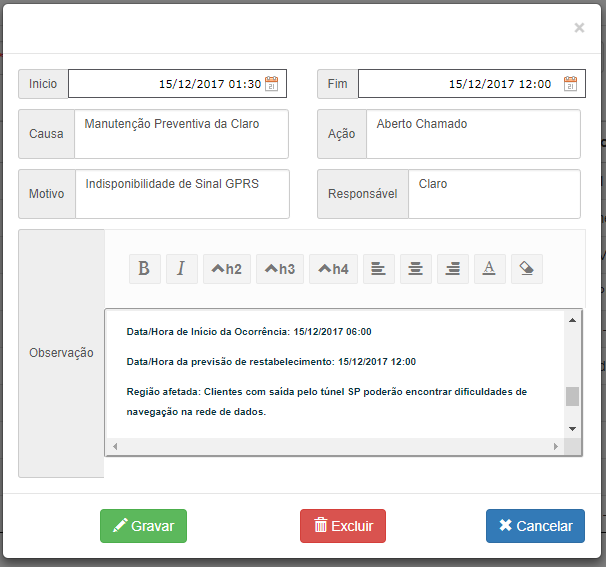
\includegraphics[width=0.5\linewidth]{images/33310_ANEXO_E_SIC_33310.png}
%	\label{fig:e_sic_33310}
%  \source{Resposta ao pedido de acesso a informação referente ao protocolo e-SIC 33310, 2017}
%\end{figure}

\clearpage
 
\section{\textit{Corpus Twitter}}

%\section{Redes Sociais}
%\label{sns}

%As Redes Sociais podem ser definidas como redes que possuem muitos relacionamentos, com grandes componentes conectados, altos coeficientes de agrupamento e grau de reciprocidade. Tais características, por exemplo, podem ser encontradas na rede social \textit{Facebook}\footnote{\url{https://www.facebook.com}. Acesso em 29 de outubro de 2017.}. O \textit{Twitter}\footnote{\url{https://twitter.com}. Acesso em 29 de outubro de 2017.} além de possuir as características de rede social mencionadas anteriormente, pode ser caracterizado também como uma Rede de Informações. Nesse tipo de rede a interação dominante é a disseminação de informações entre os relacionamentos, com baixo índice de reciprocidade \cite{myers2014information}.

No \textit{Twitter} as informações (\textit{tweets}) são publicadas contendo no máximo 280 caracteres; cada publicação pode receber \textit{retweets} (ser compartilhada por outros usuários), comentários (diretamente no \textit{tweet} --- \textit{replies} ---  ou de forma privada via caixa de mensagens) e \textit{likes} (indicador de quantos usuários gostaram da publicação). Além dessas funcionalidades, os \textit{tweets} podem conter menções a outros usuários (@nome do perfil) e rótulos (\#\textit{hashtag}) indicando assuntos, categorias, etc.

Devido as características citadas nos parágrafos anteriores, o \textit{Twitter} tem sido uma rede social importante para compartilhamento de informações e acontecimentos do cotidiano. Tais acontecimentos podem ser classificados como eventos sociais, capazes de descrever desde eventos rotineiros (\textit{shows}, jogos esportivos, etc.) a situações de crise (eventos de exceção --- desastres naturais, mobilizações sociais, dentre outros) \cite{zhou2014event}, \cite{atefeh2015survey}.
 
Portanto, o \textit{Twitter} foi escolhido como fonte de dados para a construção do conjunto de dados relacionados aos eventos de exceção devido ao fato de conter dados abertos sobre o cotidiano da cidade, disponibilizados em tempo real pelos cidadãos e órgãos públicos. Tais características, fazem dos \textit{tweets} uma rica fonte de dados, utilizada por inúmeros estudos que abordam problemas urbanos e de mobilidade urbana, conforme os analisados na revisão sistemática do Capítulo~\ref{revisao}.

Neste trabalho, o conjunto de dados utilizado para a identificação dos eventos de exceção é composto por \textit{tweets}, em português brasileiro, dos perfis contidos na Tabela~\ref{tab:oficialProfiles}. É importante observar que, para esse projeto de pesquisa, apenas os \textit{tweets} publicados pelas contas selecionadas são considerados, descartando os relacionados às interações (\textit{retweets} e \textit{replies}) entre perfis governamentais e não governamentais. Ou seja, os dados utilizados estão relacionados ao canal unidirecional de comunicação, não utilizamos interações dos cidadãos com as publicações realizadas pelos perfis selecionados. Com essa restrição, evitamos problemas referentes a confiabilidade dos dados, o que nos permite focarmos na caracterização dos eventos de exceção e de seus respectivos impactos.

Sobre a seleção dos perfis, todos foram selecionados manualmente de acordo com os órgãos responsáveis por notificar eventos de exceção. Tais perfis são de caráter público, ou seja, o acesso aos \textit{tweets} não envolve questões de privacidade.

\subsection{Processo de coleta dos \textit{tweets}}

Apesar do acesso facilitado aos \textit{tweets}, a API do \textit{Twitter} limita a quantidade e frequência de requisições aos \textit{endpoints}. Devido a isso, o artefato de \textit{software} desenvolvido para coleta (na linguagem de programação Java), busca (utilizando o \textit{plugin} \textit{Twitter4J}\footnote{\url{twitter4j.org}. Acesso em 29 de outubro de 2017.}) os 3.200 \textit{tweets} mais recentes (se disponíveis) de cada conta, através do \textit{endpoint} \textit{statuses/user\_timeline}; o qual permite no máximo 180 requisições, em um intervalo de 15 minutos, com autenticação via conta de usuário\footnote{\url{https://dev.twitter.com}. Acesso em 29 de outubro de 2017.}.

Durante a coleta dos \textit{tweets}, eles são mapeados para a seguinte classe do modelo da aplicação: \textit{TweetInfo}, que contém as informações respectivas ao \textit{id}, texto da publicação, \textit{timestamp}, endereço extraído, latitude e longitude. Em seguida, o modelo é persistido no banco de dados não relacional \textit{MongoDB}\footnote{\url{https://www.mongodb.com}. Acesso em 29 de outubro de 2017.} e também no banco de dados de séries temporais \textit{Druid}\footnote{\url{http://druid.io}. Acesso em 29 de outubro de 2017.} para exploração e visualização dos dados, processo explicado na Seção~\ref{dataViz}. Os detalhes sobre o intervalo de tempo e o número de \textit{tweets} coletados constam na Tabela~\ref{tab:tweetsCollected}.

\begin{table}[!htb]
\centering
\caption{Intervalo de tempo e número de \textit{tweets} coletados}
	\label{tab:tweetsCollected}
\begin{threeparttable}
\begin{tabular}{c|c|c|c}
\toprule
\textbf {Perfil no \textit{Twitter}} &\textbf{Total de \textit{tweets}\tnote{a}}  &\textbf{ \textit{Timestamp 1\tnote{b}}} & \textbf{\textit{Timestamp 2\tnote{c}}} \\ 
\midrule
\textit{@BombeirosPMESP} & 6,632 & 2017-05-21 & 2017-12-01 \\
\hline
\textit{@CETSP\_} & 5,735 & 2017-02-20  & 2017-12-01 \\
\hline
\textit{@CPTM\_oficial} & 6,301 & 2017-04-24 & 2017-12-01 \\
\hline
\textit{@governosp}  & 6,011 & 2017-05-10 & 2017-12-01 \\
\hline
\textit{@metrosp\_oficial} & 8,621 & 2017-06-07 & 2017-12-01 \\
\hline
\textit{@Policia\_Civil}  & 3,417 & 2015-04-15 & 2017-11-30 \\
\hline
\textit{@PMESP}  & 4,365 & 2016-06-02 & 2017-11-30 \\
\hline
\textit{@saopaulo\_agora}  & 3,960 & 2016-11-18 & 2017-11-30 \\
\hline
\textit{@smtsp\_} & 1,316 & 2017-04-26 & 2017-12-01 \\
\hline
\textit{@SPCEDEC} & 1,301 & 2015-06-09 & 2017-12-01 \\
\hline
\textit{@sptrans\_} & 9,956 & 2017-06-13 & 2017-12-01 \\
\hline
\textit{@TurismoSaoPaulo} & 3,369 & 2012-06-12 & 2017-11-29 \\
\midrule
\midrule
\textbf{Total} & 60,984 & --- & --- \\
\bottomrule
\end{tabular}
\begin{tablenotes}
            \item[a] Número de \textit{tweets} coletados.
            \item[b] \textit{Timestamp} mais antigo.
            \item[c] \textit{Timestamp} mais recente.
        \end{tablenotes}
\end{threeparttable}
\source{Felipe Cordeiro Alves Dias (2019)}
\end{table}

\clearpage

\section{Correlação entre os \textit{tweets}, dados AVL e GTFS da SPTrans}
\label{corrAll}

Conforme mencionado anteriormente, após os processos de coleta e transformação os \textit{tweets} e dados da GTFS são inseridos no banco de dados não relacional \textit{MongoDB}. Após essas fases, os dados são correlacionados com o auxílio de \textit{data frames} (estrutura de dados tabular da biblioteca \textit{Pandas}\footnote{\url{https://pandas.pydata.org/pandas-docs/version/0.23.4/generated/pandas.DataFrame.html}. Acesso em 21 de janeiro de 2019.}), implementados em\textit{scripts} na linguagem de programação \textit{Python}.

Na Figura \ref{fig:caracterization_flow}, temos o processo de extração e geolocalização dos endereços contidos nos \textit{tweets}, explicado no Capítulo \ref{exp1}. O final desse processo gera um conjunto de arquivos (no formato \textit{CSV}) contendo os eventos de exceção, endereços e geolocalizações extraídas.  Em seguida, correlacionamos esses dados com a GTFS da SPTrans para então identificarmos as linhas de ônibus impactadas pelos eventos de exceção, por meio de consultas geoespaciais. Tais consultas utilizam os dados de latitude e longitude dos endereços dos eventos de exceção, além das coordenadas espaciais existentes nos arquivos \textit{shapes} e \textit{stops} da GTFS.

Uma vez que sabemos quais linhas de ônibus foram impactadas pelos eventos de exceção, utilizamos os códigos dessas linhas de ônibus e as datas (devido a sazonalidade) dos eventos para filtrar o conjunto de dados AVL que será caracterizado. Em seguida, extraímos análises descritivas das velocidades instantâneas dos ônibus, armazenadas também em arquivos no formato \textit{CSV}. Com as descrições das velocidades instantâneas conseguimos analisar se estão dentro dos padrões esperados, além de podermos extrair regras de associação. No Capítulo \ref{dataCorr} descrevemos os experimentos realizar para caracterizar os impactos dos eventos de exceção.

Por fim, é importante mencionarmos que para viabilizarmos o processamento dos dados AVL mantivemos os arquivos no formato compactado, assim como foram fornecidos pela SPTrans. Durante o processamento realizamos a leitura dos dados em memória, convertendo \textit{bytes} para \textit{string}. Uma vez em memória, dividimos e paralelizamos o processamento dos \textit{data frames} de acordo com a quantidade de núcleos existentes na máquina. Com isso, aproveitamos melhor os recursos de \textit{hardware} e disponibilizamos \textit{scripts} que podem ser facilmente integrados a estrutura de processamento de dados da SPTrans.

\begin{figure}[H]% H manda colocar exatamente nessa posição no texto (relativa aos parágrafos anterior e posterior)
	\centering
 	  \caption{Fluxograma da correlação entre os \textit{tweets}, dados AVL e GTFS da SPTrans}
		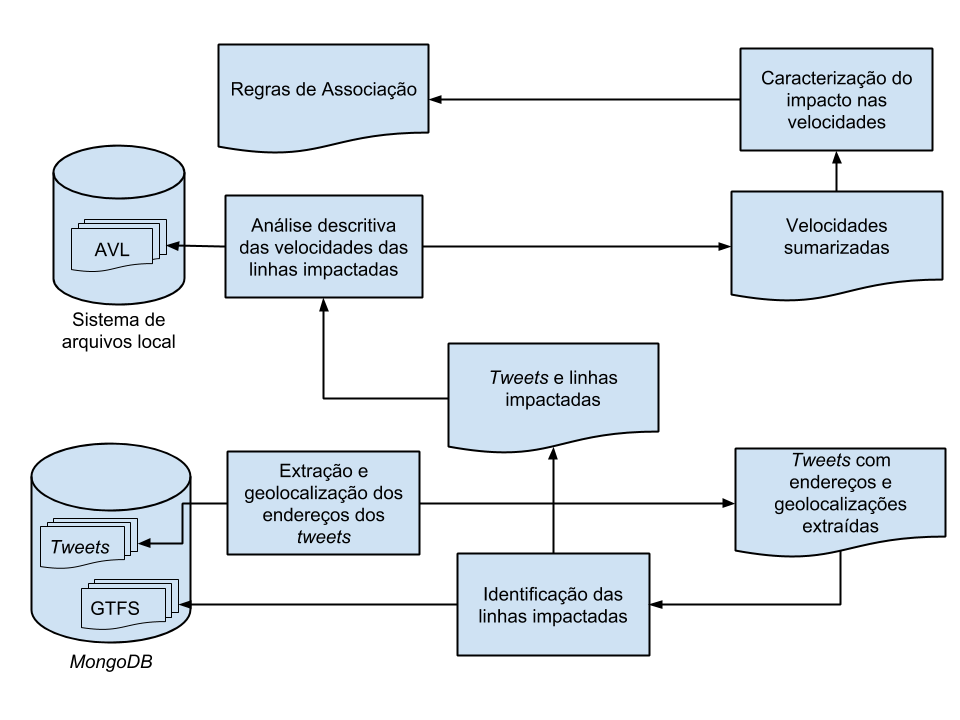
\includegraphics[width=1\linewidth]{images/caracterization_flow.png}
	\label{fig:caracterization_flow}
  \source{Felipe Cordeiro Alves Dias (2019)}
\end{figure}


%Além dos \textit{tweets} coletados, foram extraídos 625 endereços e seus respectivos dados de geolocalização. No entanto, por meio de uma análise manual percebemos dois problemas: (I) alguns endereços não foram extraídos; (II) apesar de o endereço ser extraído corretamente, encontramos geolocalizações fora do estado de São Paulo e do país. Assim, pretendemos melhorar o processo de extração dos endereços dos \textit{tweets} e o restringir a geolocalização para a região de São Paulo. 

\chapter{Exploração e visualização de grandes volumes de dados}
\label{dataViz}

Grandes volumes de dados como os relacionados ao transporte público possuem padrões complexos e demandam um sistema distribuído, apresentado neste capítulo, capaz de suportar atividades analíticas, como visualização e exploração de dados. Tais análises, são importantes para melhorar o gerenciamento, operação e planejamento do transporte público.

Dessa forma, apresentamos uma arquitetura para visualizar e explorar grandes volumes de dados (objetivo específico, apresentado na Seção \ref{objetivos}), validada com o Corpus SPTrans.  No demais, mencionamos na Seção~\ref{related_work_data_viz} alguns trabalhos referentes a visualização de dados, encontrados por meio de uma revisão não sistemática da literatura; na~\ref{druid} é descrita a arquitetura do banco de dados \textit{Druid}, principal componente da arquitetura proposta; na~\ref{arch_viz} a arquitetura em questão para processamento e exploração dos dados AVL; na~\ref{viz_case} os resultados obtidos no estudo de caso e, por fim, na~\ref{viz_case_cons} as considerações finais.

\section{Trabalhos relacionados}
\label{related_work_data_viz}

Em \cite{chen2015survey} são mencionados conceitos básicos e fluxos de visualização de dados de tráfego (dos dados brutos, pré-processamento ao mapeamento visual, construído com símbolos visuais), além de uma visão geral das técnicas e métodos de processamento de dados relacionados para processar e descrever propriedades temporais, espaciais, numéricas e categóricas de dados de tráfego.

Analogamente, em \cite{andrienko2017visual} é descrita uma tipologia de dados de tráfego, capaz de abordar suas respectivas propriedades, problemas e transformações relevantes para a análise. Além disso, são apresentadas abordagens analíticas visuais para analisar dados de tráfego de veículos, pedestres, passageiros dentro de sistemas de transporte, etc.

Por fim, no trabalho desenvolvido em \cite{seraj2017aggregation} é apresentado um novo algoritmo para mapeamento de medições coletivas para monitorar as infraestruturas de transporte terrestre e, aliviar o impacto de imprecisões do \nomenclature{GPS}{Global Positioning System}{GPS} para monitoramento contínuo de infraestruturas de transporte por meio de \textit{smart phones}.

Nenhum dos trabalhos mencionados anteriormente aborda o uso de software livre com suporte a computação distribuída, escalabilidade, tolerância a falhas, processamento em tempo real, baixa latência e visualização de grandes volumes de dados temporais. Tais requisitos, são explorados neste trabalho usando banco de dados \textit{Druid}, descrito na seção seguinte e, o \textit{Apache Superset} para analisar padrões complexos existentes nos dados AVL da SPTrans.

\section{Druid}
\label{druid}

O Druid é um banco de dados para análises exploratórias em tempo real (latências abaixo de sub-segundos) em grandes conjuntos de dados. A arquitetura distribuída do Druid é composta por um \textit{cluster} com diferentes tipos de nós (\textit{real-time, historical, broker e coordinator nodes}), que operam independentemente uns dos outros e possuem interação mínima entre eles. Existem duas dependências externas: (I) Apache Zookeeper\footnote{\url{https://zookeeper.apache.org}. Acesso em 23 de junho de 2018.}, responsável pela coordenação do cluster e (II) um sistema de gerenciamento de banco de dados relacional \nomenclature{RDBMS}{\textit{Relational Database Management Systems}}{(RDBMS --- \textit{Relational Database Management Systems}),} para armazenar parâmetros operacionais adicionais e configurações \cite{yang2014druid}.

\subsection{Real-time nodes}

\textit {Real-time nodes} são responsáveis por ingerir, indexar e consultar fluxos de eventos. Periodicamente, cada nó agenda uma tarefa em segundo plano para procurar todos os índices localmente persistentes, mesclando-os para construir \emph{blocos imutáveis de dados com todos os eventos ingeridos em um período de tempo}, conhecidos como \emph{segmentos imutáveis}, os quais podem posteriormente serem carregados para uma camada de de sistema de arquivos (\textit{deep storage}\footnote{\url{http://druid.io/docs/latest/dependencies/deep-storage.html}. Acesso em 21 de janeiro de 2019.}) \cite{yang2014druid}.

Durante os processos mencionados anteriormente não há perda de dados. Além disso, a imutabilidade dos blocos permite a consistência de leitura e um modelo de paralelização simples: \textit{historical nodes} podem simultaneamente examinar e agregar blocos imutáveis de forma não bloqueante \cite{yang2014druid}.

\subsection{Historical nodes}

Os \textit{historical nodes} são responsáveis por carregar, descartar e servir \emph{segmentos} imutáveis por meio de uma arquitetura \textit{shared-nothing} (sem um único ponto de contenção entre os nós) \cite{yang2014druid}.

\subsection{Broker nodes}

Os \textit{broker nodes} são responsáveis por receber consultas e mesclar resultados parciais dos \textit{historicals} e \textit{real-time nodes} antes de retornar um resultado final consolidado para o cliente \cite{yang2014druid}.

\subsection{Coordinator nodes}

Os \textit{coordinator nodes} são responsáveis pelo gerenciamento e distribuição dos dados nos \textit {historical nodes}, exigindo destes o carregamento, descarte e replicação dos dados \cite{yang2014druid}.

\section{Arquitetura utilizada para visualização e exploração dos dados AVL da SPTrans}
\label{arch_viz}

A Figura~\ref{fig:viz_arch} mostra a arquitetura utilizada no estudo de caso deste capítulo, composta pelos componentes do \textit{Druid} em conjunto com o módulo \textit {Apache Superset}\footnote{\url{https://superset.incubator.apache.org}. Acesso em 23 de junho de 2018.} --- software de código aberto para exploração e análise de dados, nativamente integrado ao \textit{Druid}. Nesta arquitetura, dois fluxos para processamento de dados também são elencados: (I) em lote, para análises mais complexas (correlações, extrações de \textit{features}, etc.) e (II) em tempo real, necessário devido ao requisito de análises tempestivas, normalmente envolvendo agregação e sumarização dos dados.

\begin{figure}[!htb]% H manda colocar exatamente nessa posição no texto (relativa aos parágrafos anterior e posterior)
	\centering
 	  \caption{Arquitetura usada no estudo de caso para visualização e exploração dos dados AVL da SPTrans}
		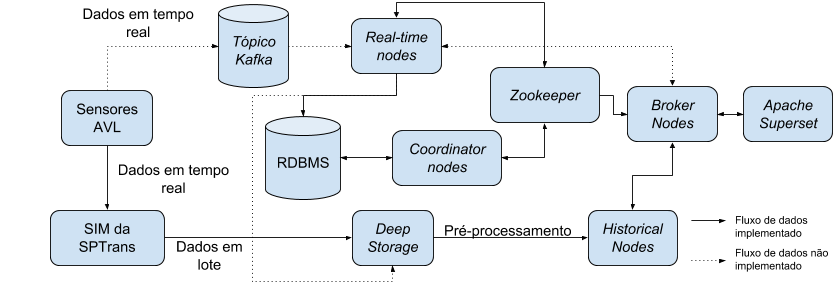
\includegraphics[width=1\linewidth]{images/viz_arch_pt.png}
	\label{fig:viz_arch}
\source{Felipe Cordeiro Alves Dias (2019)}
\end{figure}

O fluxo de processamento em lote é executado a partir dos dados extraídos do sistema de monitoramento da \textit{SPTrans}, os quais são ingeridos nos \textit{historical nodes} 
%(a latência de ingestão máxima medida é 22.914,43 eventos / segundo / núcleo, com uma fonte de dados com 30 dimensões e 19 métricas \cite{yang2014druid}) 
e disponibilizados para o \textit{Apache Superset} por meio dos \textit{broker nodes}. 
%(que tem uma latência média de consulta de aproximadamente 550 milissegundos \cite{yang2014druid}).
É importante observar que o fluxo de processamento em lote é o fluxo de dados implementado neste estudo de caso.

Na arquitetura ilustrada na Figura~\ref{fig:viz_arch}, o fluxo de dados em tempo real refere-se a uma proposta alvo para a \textit{SPTrans}, a fim de permitir a exploração e visualização dos dados dos ônibus da cidade de São Paulo em tempo real. Nesta proposta, os tópicos do \textit{Apache Kafka}\footnote{\url{https://kafka.apache.org}. Acesso em 21 de janeiro de 2019.} (plataforma distribuída para processamento de fluxos de dados) desempenham o papel de receptores do fluxo de dados, a partir dos quais os dados podem seguir tanto o processamento em tempo real quanto em lote.

Por fim, é importante observar que em ambos os fluxos há um estágio de pré-processamento de dados, para adequar os dados AVL as especificações exigidas para a ingestão no \textit{Druid} (o que adiciona atraso no fluxo de processamento).

\section{Estudo de caso com os dados AVL da SPTrans}
\label{viz_case}

Grandes volumes de dados podem conter padrões complexos e difíceis de serem identificados. Devido a isso, é importante construir visualizações auxiliares para o processo de análise de dados. Com este propósito, usamos o \textit{Apache Superset}\footnote{\url{https://superset.incubator.apache.org}. Acesso em 29 de junho de 2018}, com suporte nativo ao \textit{Druid}, para exploração e visualização do \textit{corpus} da SPTrans. As figuras~\ref{fig:analysis_by_bus_lines},~\ref{fig:pizza_bus},~\ref{fig:only_one_bus_map} e~\ref{fig:buses_map} são exemplos de algumas visualizações construídas a partir dos dados de janeiro das linhas de ônibus selecionadas aleatoriamente.

A Figura~\ref{fig:analysis_by_bus_lines} ilustra uma série temporal referente à quantidade de dados enviados por ônibus selecionados aleatoriamente, referentes a janeiro de 2017. Com esta visualização é possível observar, por exemplo, a oscilação da quantidade de dados enviados, assim como os picos de maior e menor volume de envio de dados e janelas de tempo com dados ausentes. Tais oscilações podem indicar problemas relacionados a essas viagens, como eventos de exceção decorrentes de paralisação sindical (redução da frota de ônibus), atos de violência como os de 2006 que incendiaram noventa ônibus em São Paulo\footnote{\url{https://pt.wikipedia.org/wiki/Atos\_de_violência\_organizada\_no\_Brasil\_em\_2006}. Acesso em 21 de janeiro de 2019} e os de 2019 com 21 ônibus incendiados no Ceará\footnote{\url{https://pt.wikipedia.org/wiki/Atentados_no_Ceará_em_2019}. Acesso em 21 de janeiro de 2019.}.

\begin{figure}[!htb]% H manda colocar exatamente nessa posição no texto (relativa aos parágrafos anterior e posterior)
	\centering
 	  \caption{Quantidade de dados enviados por dia  por ônibus (selecionados aleatoriamente) em janeiro de 2017}
		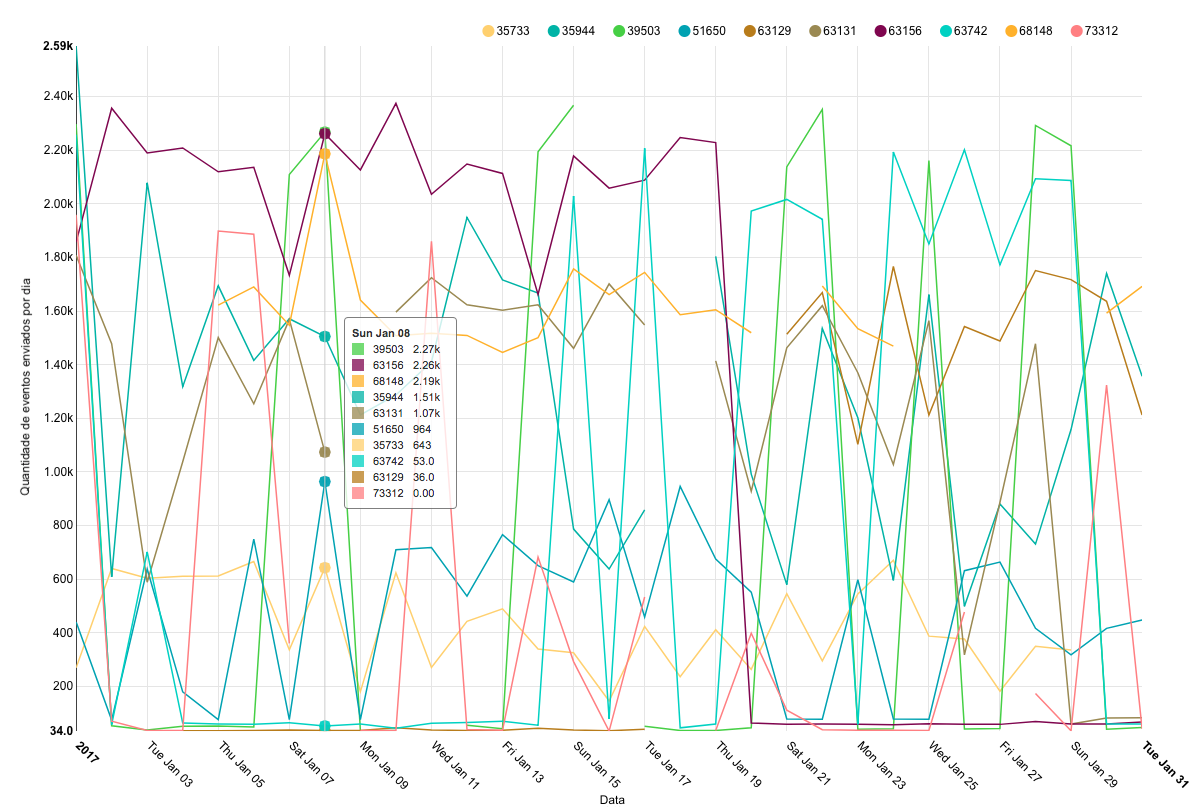
\includegraphics[width=1\linewidth]{images/analysis_by_bus_lines_pt.png}
	\label{fig:analysis_by_bus_lines}
\source{Felipe Cordeiro Alves Dias (2019)}
\end{figure}

A Figura~\ref{fig:pizza_bus}, representa a distribuição da quantidade de dados enviados em janeiro, a partir de uma amostra aleatória de linhas ônibus. Nessa figura é possível analisar que a distribuição da quantidade de dados enviados não é normalizada, ou seja, existem ônibus que normalmente enviam mais dados do que os demais. Há muitas razões possíveis para isso, por exemplo: viagens de ônibus mais longas que outras, regiões com diferenças climáticas; módulos AVL desatualizados; maior quantidade de ônibus em uma determinada linha, etc.

\begin{figure}[!htb]% H manda colocar exatamente nessa posição no texto (relativa aos parágrafos anterior e posterior)
	\centering
 	  \caption{Distribuição da quantidade de dados enviados por ônibus (selecionados aleatoriamente) em janeiro de 2017}
		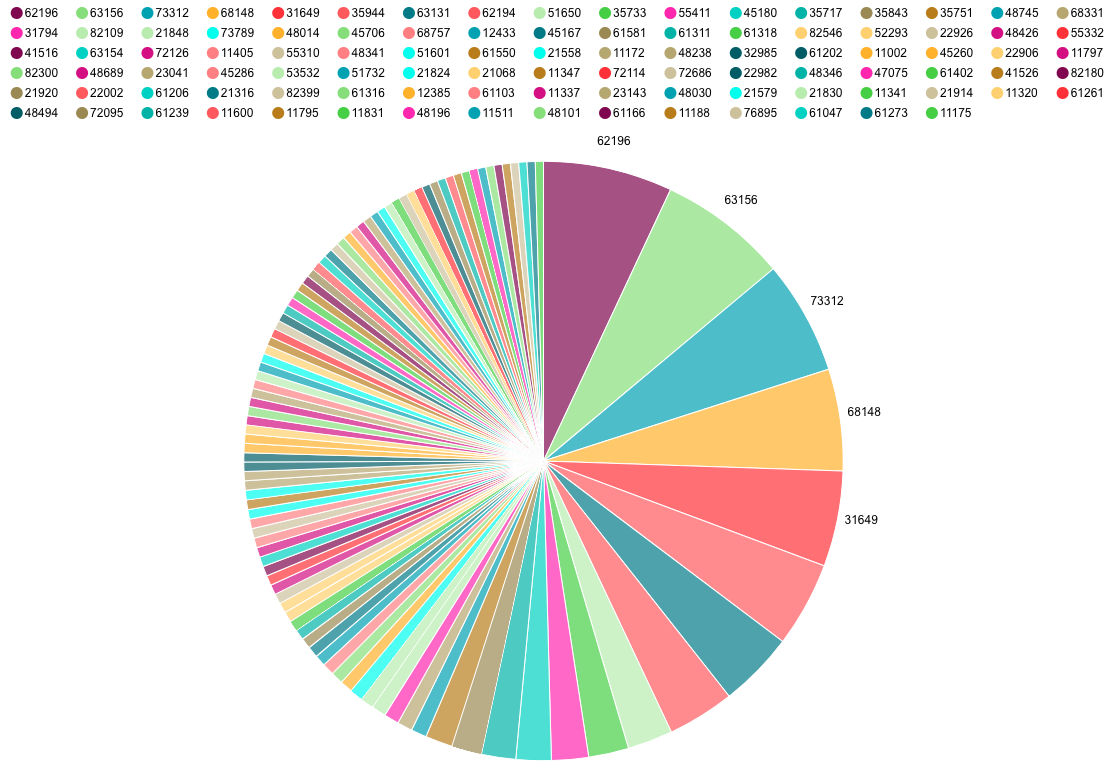
\includegraphics[width=1\linewidth]{images/pizza_bus.png}
	\label{fig:pizza_bus}
\source{Felipe Cordeiro Alves Dias (2019)}
\end{figure}

Finalmente, os mapas exibidos pelas figuras~\ref {fig:buses_map} e~\ref{fig:only_one_bus_map} ajudam a identificar a localização a partir da qual os dados estão sendo enviados, permitindo visualizar possíveis pontos de falhas durante a transmissão desses dados. O primeiro mapa, respectivamente, refere-se à rota de uma única linha de ônibus e o segundo de todas as rotas; em ambos os casos, referentes aos dados de janeiro. Além disso, na Figura~\ref {fig:buses_map}, é possível observar a segregação urbana da cidade, devido ao fato de algumas regiões terem uma maior densidade de dados enviados, o que também indica regiões de maior tráfego, nas quais eventos de exceção teriam maior impacto.

\begin{figure}[!htb]% H manda colocar exatamente nessa posição no texto (relativa aos parágrafos anterior e posterior)
	\centering
 	  \caption{Localizações enviadas em Janeiro de 2017 de uma linha de ônibus selecionada aleatoriamente}
		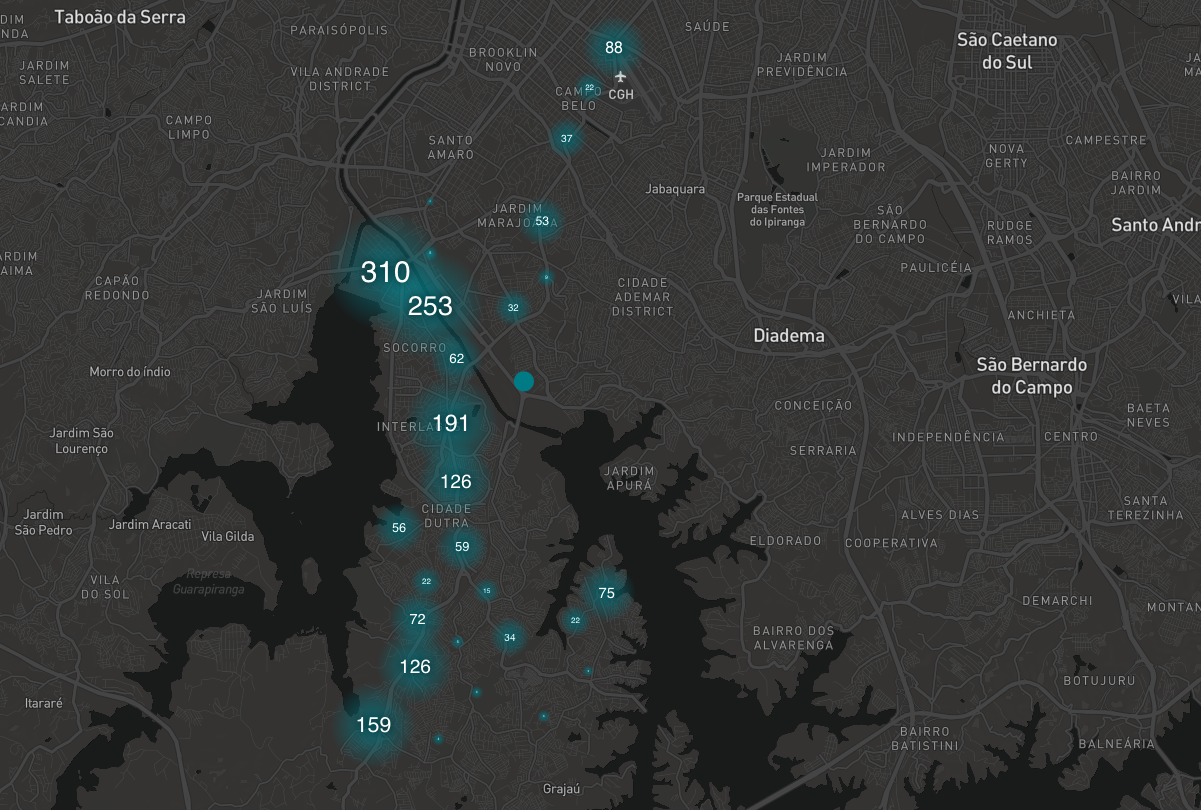
\includegraphics[width=0.95\linewidth]{images/only_one_bus_map.png}
	\label{fig:only_one_bus_map}
 \source{Felipe Cordeiro Alves Dias (2019)}
\end{figure}

\begin{figure}[!htb]% H manda colocar exatamente nessa posição no texto (relativa aos parágrafos anterior e posterior)
	\centering
 	  \caption{Localizações dos ônibus referente a movimentação de Janeiro de 2017}
		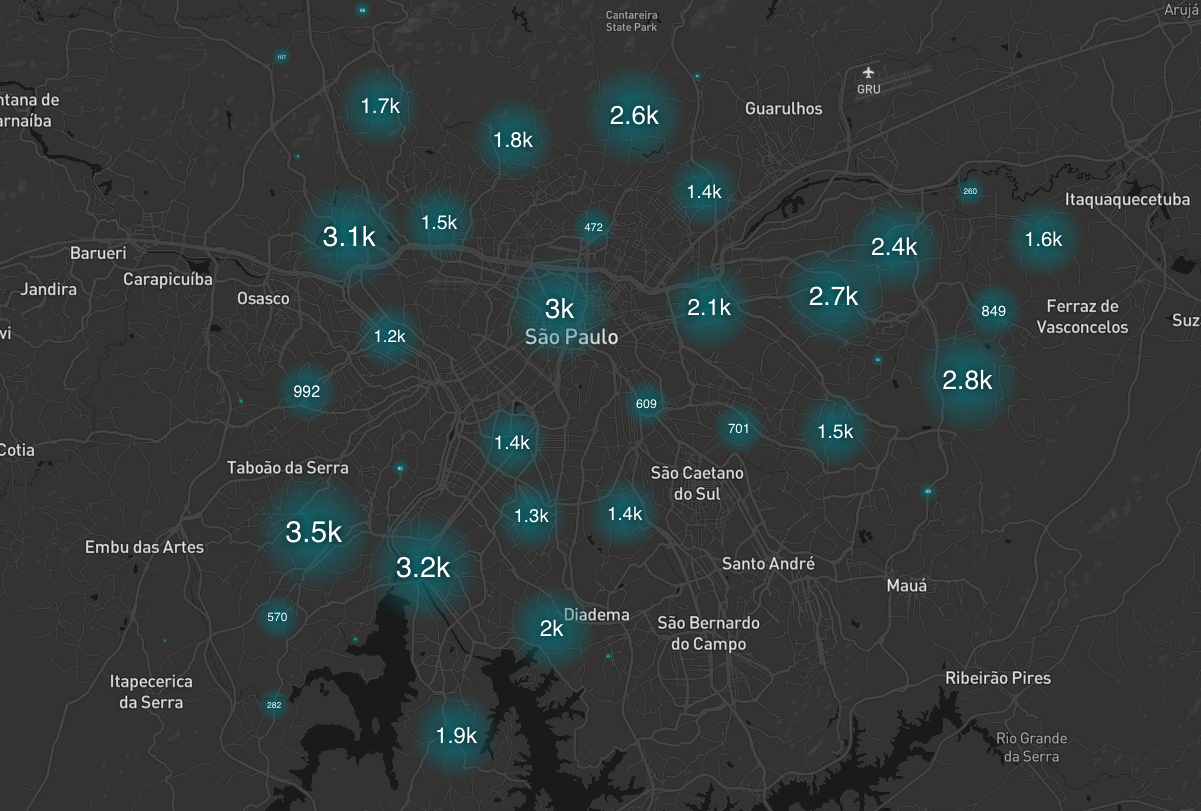
\includegraphics[width=0.95\linewidth]{images/buses_map.png}
	\label{fig:buses_map}
	\source{Felipe Cordeiro Alves Dias (2019)}
\end{figure}

\section{Consideração sobre a arquitetura utilizada para exploração e visualização dos dados AVL da SPTrans}
\label{viz_case_cons}

Este capítulo apresentou um estudo de caso relacionado à visualização de grandes conjuntos de dados, utilizando dados dos ônibus da cidade de São Paulo. Também, mostramos que é possível encontrar padrões complexos e incomuns e possíveis eventos de exceção em grandes conjuntos de dados por meio da visualização. O \textit{Druid} e o \textit{Apache Superset} demonstraram suporte a agregação, exploração e visualização de grandes conjuntos de dados. 
%Como trabalho futuro, pretendemos implementar o fluxo de dados mencionado na Figura~\ref{fig:viz_arch}, em um cenário de exploração e visualização de dados \textit{near real time}.


\chapter{Identificação de linhas de ônibus impactadas por eventos de exceção}
\label{exp1}

O objetivo geral desse projeto de pesquisa é a caracterização de eventos de exceção e de seus respectivos impactos no sistema de transporte público por ônibus da cidade de São Paulo, conforme mencionado na Seção \ref{objetivos}. Portanto, para alcançarmos o objetivo proposto precisamos de uma metodologia capaz de encontrar as linhas de ônibus que são impactadas por eventos de exceção, para então explorarmos as características desse impacto. Sendo assim, apresentamos neste capítulo uma metodologia baseada em \textit{tweets} para identificar linhas de ônibus impactadas por eventos de exceção. De acordo com a Figura~\ref{fig:tweet_based_methodology}, a metodologia, explicada em detalhes nas seções seguintes, é composta por:

\begin{enumerate*}
\item Uma base de dados de \textit{tweets} --- \textit{Copus Twitter}.
\item Pré-processamento dos \textit{tweets} existentes no conjunto de dados.
\item Extração de localização e geolocalização.
\item Processamento dos \textit{tweets}.
\item Criação de um modelo de classificação de \textit{tweets} em classes de eventos de exceção.
\item Identificação das linhas impactadas --- por meio de consultas a base GTFS existente no \textit{Corpus SPTrans} --- a partir de um raio de cada evento de exceção.
\end{enumerate*}

\begin{figure}[!htb]
	\centering
 	  \caption{Fluxograma da metodologia baseada em \textit{tweets} para encontrar linhas de ônibus impactadas por eventos de exceção na cidade de São Paulo}
		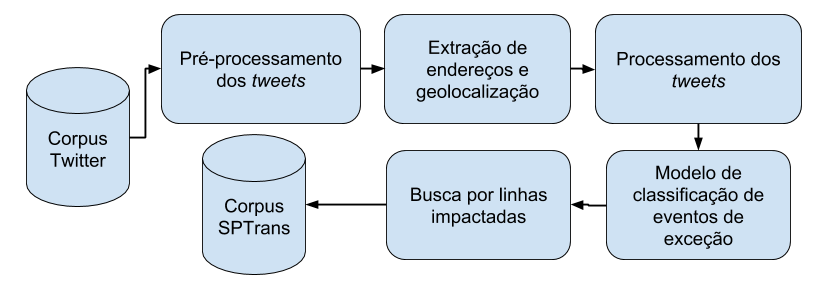
\includegraphics[width=0.7\linewidth]{images/tweet_based_methodology_pt.png}
	\label{fig:tweet_based_methodology}
	\source{Felipe Cordeiro Alves Dias (2019)}
\end{figure}

\section{Pré-processamento}
\label{preprocessing}

Numa pré-análise do \textit{Corpus Twitter}, podemos averiguar que os \textit{tweets} publicados pelos perfis selecionados evitam o uso de gírias, abreviações, erros de digitação; conforme consta nos \textit{tweets} de exemplo contidos no trecho de código em \textit{json}, no apêndice~\ref{tweetsSample}.  Isso diferencia tais \textit{tweets} dos \textit{tweets} publicados por usuários comuns do \textit{Twitter}, que contém erros gramaticais, de sintaxe e que normalmente dependem de análise contextual para que possam ser interpretados.

Apesar disso, com base na literatura analisada (\cite{Steiger2015Census}, \cite{Middleton2014}, \cite{Kobdani2010}, \cite{Setiawan2017},  \cite{Zagal2016}), as seguintes etapas de pré-processamento são necessárias para remoção de ruído e redução da dimensão do espaço de \textit{features} e foram realizadas para o \textit{Corpus Twitter}:

\begin{itemize}
\item \textit{Case folding}: processamento de normalização de todas as letras do texto (de A-Z) para minúsculas.
%\item \textit{\textbf{Tokenization}}: processamento realizado para obtenção das palavras  (\textit{tokens}) que compõem uma sentença, inclui a remoção de números, pontuações e caracteres que não pertencem ao alfabeto \cite{Setiawan2017}.  
%\item \textbf{Remoção de} \textit{\textbf{stopwords}}: processamento para remoção do conjunto de \textit{tokens} de palavras sem significado ou importância \cite{Setiawan2017}, o que reduz a quantidade de ruído do conteúdo \textit{tweet} \cite{Steiger2015Census}.
%\item \textit{\textbf{Stemming}}: processamento para encontrar a raiz de uma palavra, removendo sufixos e prefixos (no caso do Português Brasileiro) das palavras derivadas \cite{Setiawan2017}.
\item Remoção de \nomenclature{URL}{\textit{Uniform Resource Locator}} \textit{URLs} e menções a outros \textit{tweets}.
\item Remoção de acentos, \textit{emoticons} e pontuações substituídas por espaços vazios.
%\item Correção erros de digitação por meio de uma função de mapeamento
\item \textit{Stemming} (conceito explicado na Seção \ref{nlp})  --- realizado neste trabalho na fase de processamento mencionada na Seção~\ref{processing}, com o objetivo de não afetar o processo de extração de endereços. 
\end{itemize}

Além disso, é importante observar que (I) as informações referentes a data e hora mencionadas no conteúdo dos \textit{tweets} (\textit{stopwords} específicas do domínio) são removidas do texto original. As informações de data e hora consideradas para os eventos de exceção são as contidas nos metadados dos \textit{tweets}, posto que ao analisarmos os \textit{tweets} verificamos que as informações de data e hora contidas no texto normalmente são referentes a eventos futuros, os quais não são considerados por este trabalho; (II) os \textit{retweets} não estão presentes no \textit{Corpus Twitter}; (III) no pré-processamento não há transformação do conteúdo dos \textit{tweets}, embora trabalhos como os relacionados a identificação de sentimentos usem esse meio para transformar \textit{emoticons} nos sentimentos que eles representam \cite{Zagal2016}; (IV) as \textit {hashtags} não são removidas dos \textit{tweets} originais, pois são importantes para a classificação dos eventos de exceção.

Uma atenção especial foi dada às \textit{hashtags}, que são relevantes para a classificação de eventos de exceção, mas adicionam ruído à fase de extração de endereços. Para mitigar o problema, \textit{hashtags} são identificadas e substituídas por espaços vazios no processo de extração de endereço. Além disso, é importante notar que as \textit{hashtags} não são removias dos \textit{tweets} originais.

\section{Extração de endereço e geolocalização}

Analisando o conteúdo dos \textit{tweets} das contas selecionadas, é possível observar que os textos publicados seguem um determinado padrão e, portanto, são semi-estruturados. Ante a isso, usamos a seguinte expressão regular para extrair os endereços presentes no conteúdo dos \textit{tweets}:
%
\begin{equation}
ER = \lbrace L_1 | S_1 | L_2 | S_2 | \dots | L_n | S_n \rbrace \lbrace [a-z\grave{A}-\ddot{y}\_] + \rbrace
\end{equation}

A expressão anterior é dividida em dois conjuntos, no primeiro ($\lbrace L_1 | S_1 | L_2 | S_2 | \newline \dots | L_n | S_n \rbrace $), (L --- logradouros) e (S --- acrônimos de espaços públicos) são concatenados para especificar um filtro e identificar sequências inicializadas com espaços públicos ou seus respectivos acrônimos. No segundo conjunto ($\lbrace [a-z\grave{A}-\ddot{y}\_] + \rbrace $), é especificado um filtro para identificar um conjunto de palavras após L ou S, que são candidatas a compor o endereço desejado.

Essas palavras são candidatas porque é difícil saber quantas palavras após L ou S pertencem ao endereço, no entanto, as contas selecionadas publicam padrões visíveis após os endereços. Como consequência, um método possível para encontrar o endereço desejado é a remoção desses padrões após o início do endereço.

Após a extração do endereço, é necessário geolocalizar o endereço encontrado --- apenas 1,5 \% de \textit {tweets} têm geolocalização \cite{niu2016community} --- o que é possível, por exemplo, usando a \nomenclature{API}{\textit{Application Programming Interface}}{API} de geocodificação do Google Maps\footnote {\url {https://developers.google.com/maps/documentation/geocoding}. Acesso em 11 de Abril de 2018.}. Os parâmetros de URL utilizados neste trabalho para chamar a API mencionada anteriormente são: (I) \emph {address} --- o endereço desejado; (II) \emph {bounds} --- uma caixa delimitadora para o resultado retornado, a qual é especificada pelas coordenadas de latitude / longitude dos cantos sudoeste e nordeste de São Paulo; (III) \emph {region} --- código da região com dois caracteres, por exemplo, \textit{br} para o Brasil e (IV) \emph {token} --- \textit{token} usado na autenticação da API.

Em seguida, a resposta HTTP é processada para obter os valores da localização (que contém informações de latitude e longitude) e o \emph{endereço formatado}. É importante observar que os \textit{tokens} do endereço extraído (\emph{endereço não formatado}) são \textit{stopwords} específicas do \textit{corpus} em caso de alta frequência de eventos de exceção localizados neste endereço, devido ao fato de que nesse cenário elas são tratados como \textit{features} relevantes para o modelo de classificação. Portanto, os \textit{tokens} dos endereços extraídos são armazenados para serem removidos na fase de processamento dos \textit{tweets}.

\section{Processamento de \textit{tweets}}
\label{processing}

Nesta fase, os \textit {tweets} são preparados para serem usados para treinar um modelo de classificação de eventos de exceção; neste momento, todos os \textit {tweets} já foram pré-processados. Conforme mencionado na seção anterior, nesta fase os \textit{tokens} dos endereços extraídos armazenados são removidos para redução de ruído e as \textit{stopwords} do português brasileiro filtradas\footnote{\textit{Stopwords} do português brasileiro obtidas da \nomenclature{NLTK}{Natural Language Toolkit}{NLTK ---} \url{https://www.nltk.org}. Acesso em 19 de Abril de 2018.} e todos os demais \textit{tokens}  processados por um \textit{stemmer} para o  português brasileiro\footnote{RSLP Stemmer --- \url {http://www.nltk.org/\_modules/nltk/stem/rslp.html}. Acesso em 19 de Abril de 2018.} para reduzir a dimensão do espaço de \textit{features}.

\section{Classificação manual do Corpus \textit{Twitter}}
\label{manualClassification}

Encontrar eventos de exceção envolve a identificação de eventos relacionados a uma exceção, o que é possível por meio de classificação de \textit{tweets} (manualmente ou de forma autônoma). De acordo com a revisão sistemática apresentada no Capítulo~\ref{revisao}, as seguintes classes podem ser usadas para classificar eventos de exceção:

\begin{enumerate}
\item \textbf{Acidentes}.
\begin{enumerate}
\item Acidentes nas estações transporte \cite{Itoh2016}.
\item Incêndio \cite{Itoh2016}.
\end{enumerate}

\item \textbf{Espaço-temporais}.
\begin{enumerate}
\item Dia da semana \cite{Chen2016}.
\item Hora do dia \cite{Chen2016}.
\end{enumerate}

\item \textbf{Eventos sociais}.
\begin{enumerate}
\item Feiras de rua \cite{Chen2016}.
\item Festivais \cite{Chen2016}, \cite{Lecue2014}.
\item Jogos esportivos \cite{Chen2016}, \cite{Gal-Tzur2014}.
\item Passeatas e maratonas \cite{Chen2016}, \cite{Itoh2016}.
\end{enumerate}

\item \textbf{Eventos urbanos}.
\begin{enumerate}
\item Relacionados ao tráfego \cite{Chen2016}, \cite{Lecue2014}.
\end{enumerate}

\item \textbf{Desastres naturais}.
\begin{enumerate}
\item Tempestades \cite{Itoh2016}.
\item Terremoto \cite{Itoh2016}.
\item Tufões \cite{Itoh2016}.
\end{enumerate}

\item \textbf{Meteorológicos}.
\begin{enumerate}
\item Dia claro, nublado, chuvoso, nevando, com neblina \cite{Chen2016}.
\item Temperatura do ar \cite{Chen2016}.
\end{enumerate}
\end{enumerate}

Após o estudo do domínio do conhecimento, por meio da revisão sistemática para coletar as classes de exceção, o Corpus Twitter, contendo 60.984, foi classificado manualmente de acordo com suas respectivas classes. Tal conjunto foi usado para treinar o modelo de classificação de \textit{tweets} em classes de eventos de exceção. 

\section{Modelo de classificação de \textit{tweets} relacionados a eventos de exceção}
\label{model}

O corpus obtido da fase de processamento de \textit {tweets} é representado por um \textit{bag-of-words} que contém vetores de \textit{features} criados usando a medida \textit{Term Frequency - Inverse Document Frequency}\nomenclature{TF-IDF}{\textit{Term Frequency - Inverse Document Frequency}} (TF-IDF). A bag-of-words é particionada aleatoriamente em conjuntos de treinamento (60\%) e teste (40\%), os quais são entradas para os algoritmos de classificação mencionados na Seção~\ref{supervisionedLearning}.

\section{Encontrando linhas de ônibus afetadas por eventos de exceção}

Para encontrar as linhas de ônibus afetadas por eventos de exceção, é necessário correlacionar latitude e longitude dos eventos de exceção com as \textit{stops} da GTFS da SPTrans. Como mencionado anteriormente, os dados referentes as \textit{stops} contém os locais individuais em que os veículos pegam ou deixam passageiros, incluindo coordenadas de latitude e longitude.

De acordo com a Seção~\ref{CorpusSPTrans}, todas as coordenadas são armazenadas em pares no formato \textit{legacy} e em coleções com índices geoespaciais. Assim, é possível usar a função \textit{\$near} do MongoDB\footnote {\url{https://docs.mongodb.com/manual/reference/operator/query/near}. Acesso em 18 de Maio de 2018.} para encontrar as \textit{stops} próximas às coordenadas do evento de exceção. Como consequência da GTFS, o \textit{stop\_id} faz parte dos atributos contidos no arquivo de \textit{stops}, referindo-se a um código de parada de ônibus com o qual é possível correlacioná-lo com as bases \textit{stop\_times} e \textit{lines} (por meio do atributo \textit{trip\_id} existente em \textit{stops}) para obter mais detalhes sobre a direção da linha de ônibus, identificação, etc.

\section{Resultados}
	
A metodologia foi aplicada ao Corpus Twitter\footnote{Conjunto de dados disponível em: \url{https://drive.google.com/drive/folders/16NIevLsBR0A45UHdPDvv2lZZx6gF4R0p?usp=sharing}. Acesso em 8 de Setembro de 2018.}. No final do pré-processamento e processamento dos \textit{tweets}, o corpus obteve 414,637 palavras, com um vocabulário de 13,915 palavras. O comprimento máximo das sentenças do conjunto de dados é 19, sua respectiva variação é ilustrada pela Figura~\ref{fig:corpus_metrics}.
 
\begin{figure}[!htb]
	\centering
 	  \caption{Histograma da variação dos tamanhos das sentenças dos \textit{tweets} existentes no \textit{Corpus Twitter}}
		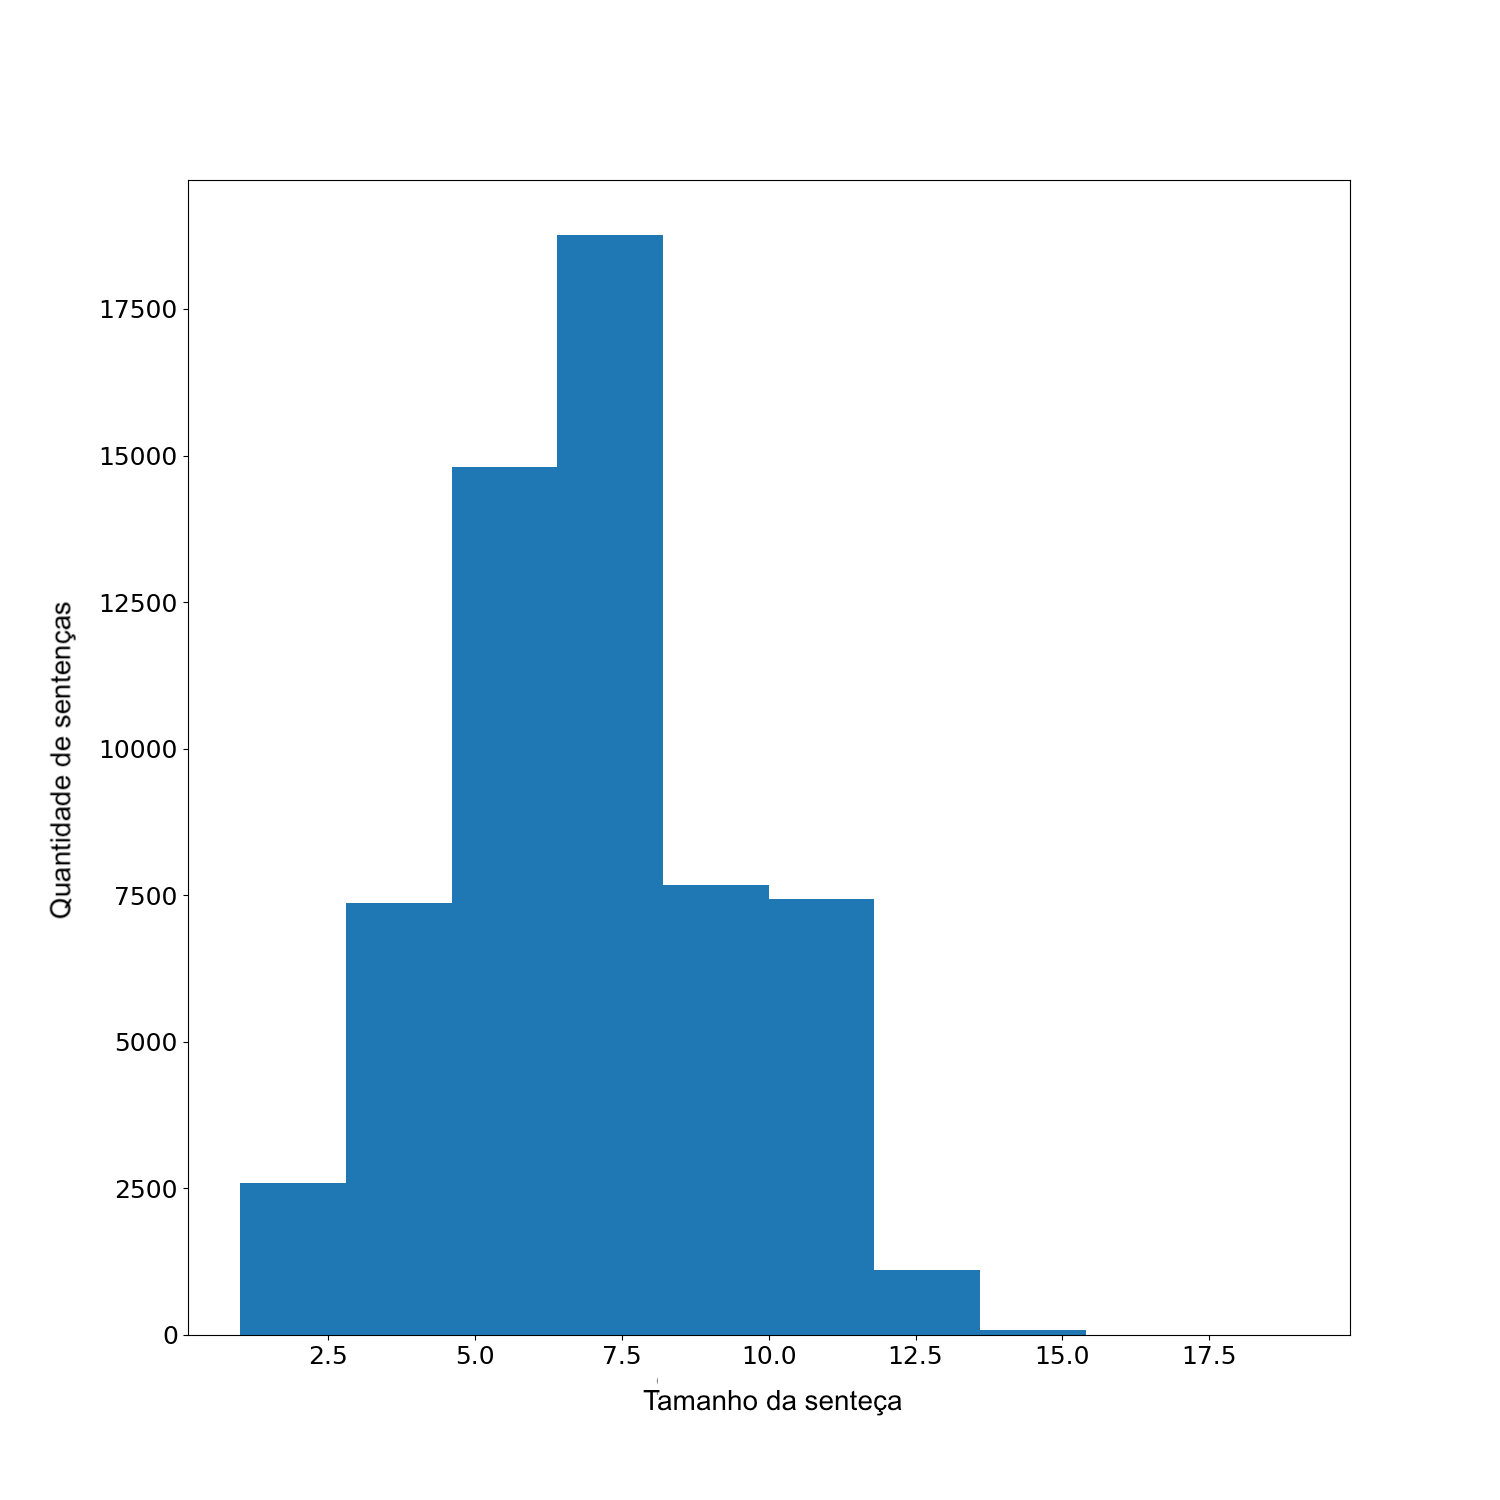
\includegraphics[width=1\linewidth]{images/corpus_metrics_pt.png}
	\label{fig:corpus_metrics}
	\source{Felipe Cordeiro Alves Dias (2019)}
\end{figure}

Todos os \textit{tweets} existentes no \textit{Corpus Twitter} foram classificados manualmente de acordo com os eventos de exceção identificados. Este conjunto de dados é composto pelas seguintes classes: Acidente, Irrelevante --- quando o \textit{tweet} não é um evento de exceção, Desastre Natural, Evento Social e Evento Urbano. A Figura~\ref{fig:tweets_distribution} ilustra a distribuição das classes de eventos de exceção em cada conta selecionada.

\begin{figure}[!htb]
	\centering
 	  \caption{Distribuição das classes dos eventos de exceção do Corpus Twitter}
		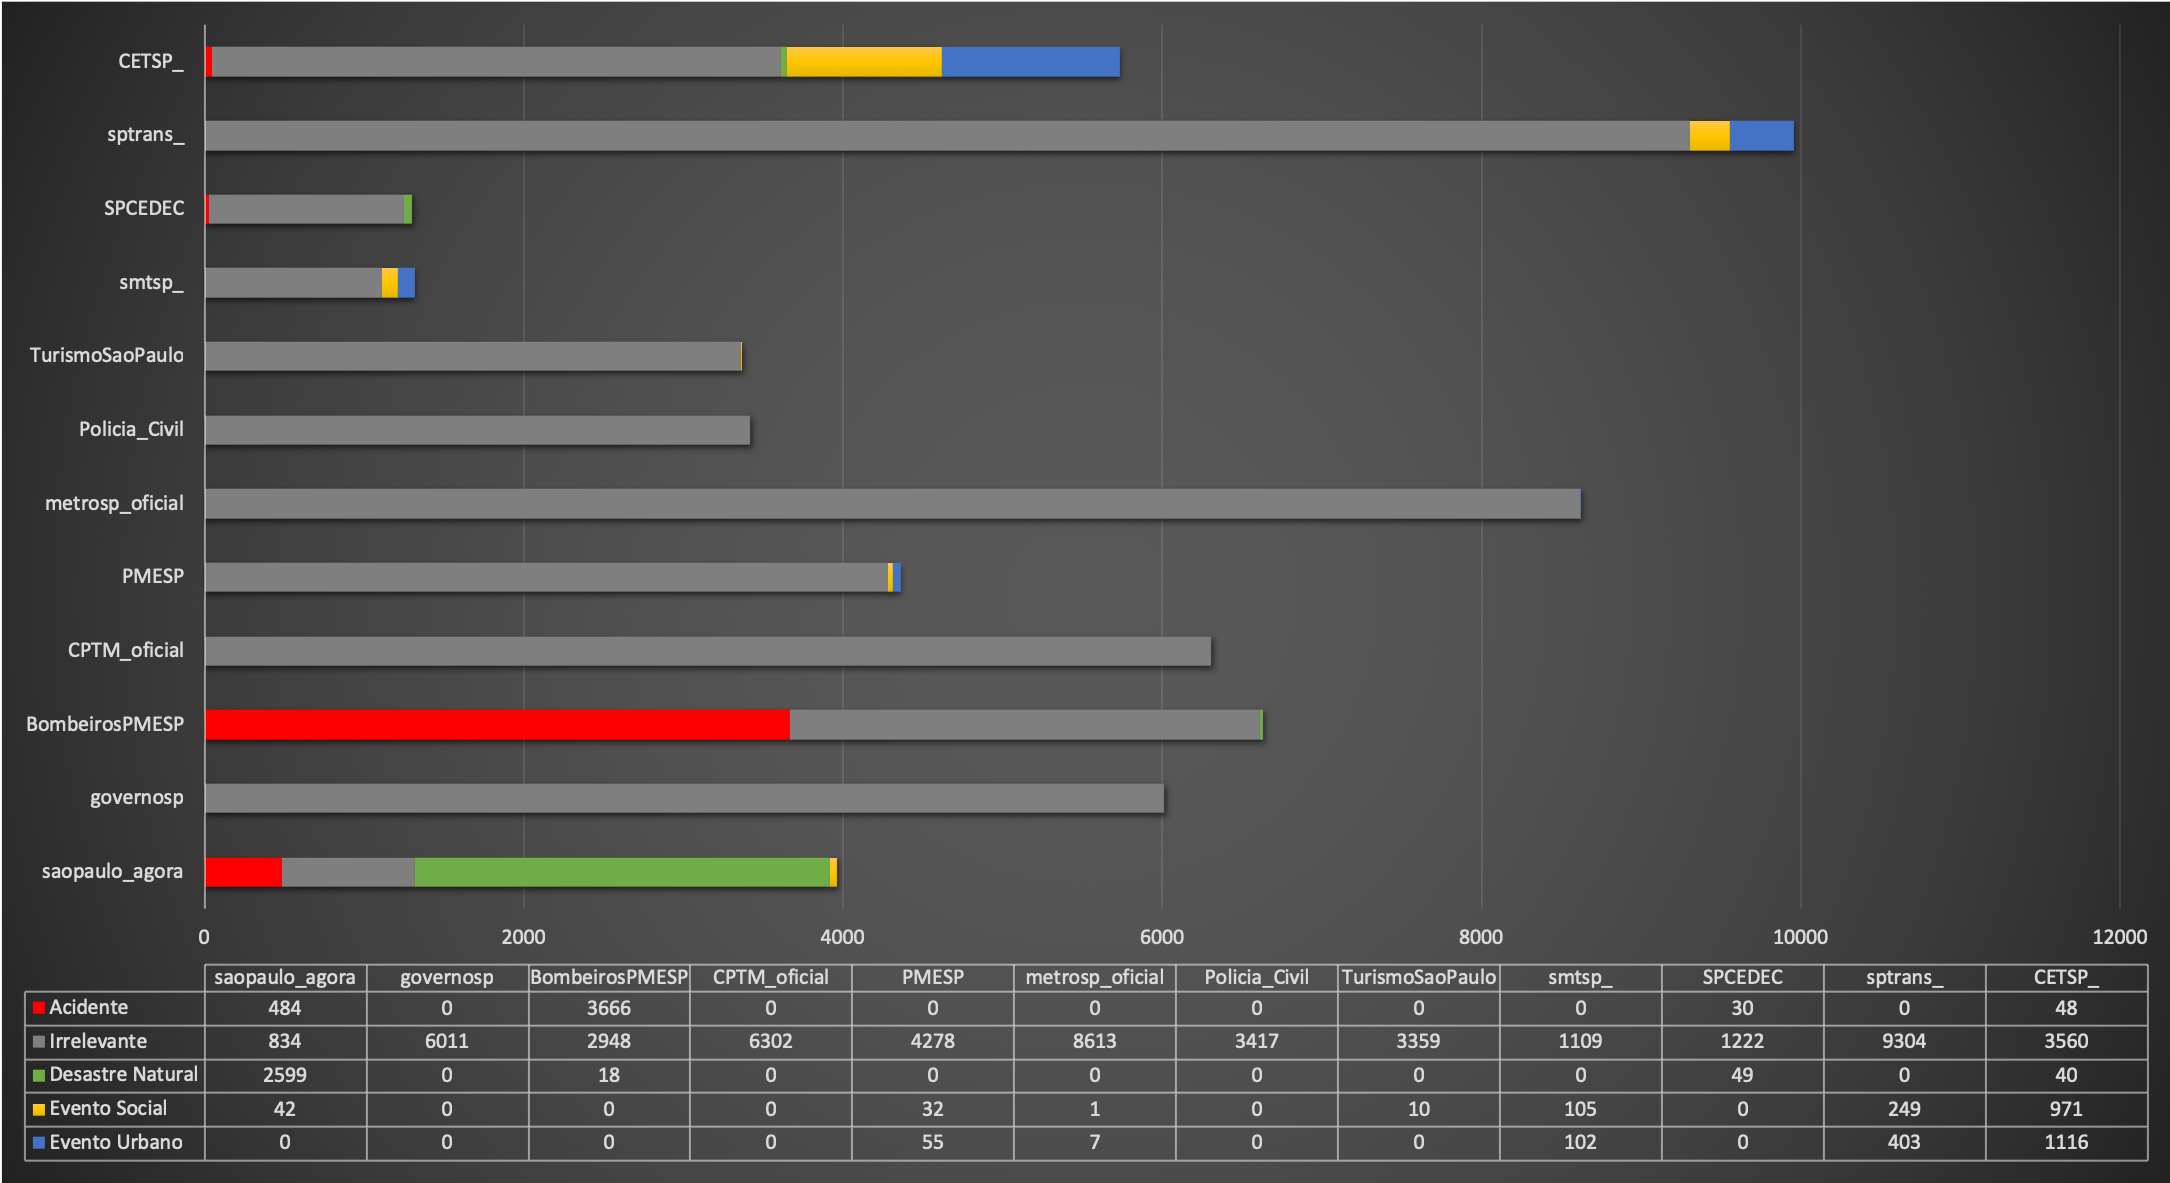
\includegraphics[width=1\linewidth]{images/tweets_distribution_pt.png}
	\label{fig:tweets_distribution}
	\source{Felipe Cordeiro Alves Dias (2019)}
\end{figure}

Esse conjunto de dados rotulado foi usado para treinar modelos de classificação de eventos de exceção, com base em uma \textit{bag-of-words}, descrita na Seção~\ref{model}. De acordo com a Tabela~\ref{tab:metrics}, o modelo que usa o algoritmo \textit{Perceptron Multicamadas} obteve maior acurácia para a tarefa de classificar os \textit{tweets} em eventos de exceção. A matriz de confusão relacionada ao algoritmo \textit{Perceptron Multicamadas} é ilustrada pela Figura~\ref{fig:confusion_matrix_mlp}, as matrizes de confusão dos demais algoritmos podem ser consultadas no Apêndice~\ref{apendiceE}.

\begin{table}[!htb]
\centering
\caption {Métricas das avaliações dos algoritmos utilizados para classificação dos \textit{tweets} em eventos de exceção}
\label {tab:metrics}
\begin{tabular}{c|c|c|c|c}
\toprule
\textbf{Algoritmo} & \textbf{ACC} & \textbf{PPV} & \textbf{TPR} & \textbf{\textit{f1-score}} \\
\midrule
\textit{Naive Bayes} Complementar & 0,941 & 0,949 & 0,941 & 0,944 \\
\hline
Árvore de Decisão & 0,965 & 0,965 & 0,965 & 0,965 \\
\hline
K-ésimo Vizinho mais Próximo & 0,970 & 0,971 & 0,970 & 0,970 \\
\hline
Regressão Logística & 0,969 & 0,968 & 0,969 & 0,968 \\
\hline
Perceptron multicamadas & \textit{0,973} & \textit{0,972} & \textit{0,973} & \textit{0,972} \\
\hline
\textit{Naive Bayes} Multinomial & 0,953 & 0,952 & 0,953 & 0,949 \\
\hline
Floresta Aleatória & 0,970 & 0,970 & 0,970 & 0,970 \\
\hline
Máquina de Vetores de Suporte & 0,833 & 0,694 & 0,833 & 0,757 \\
\bottomrule
\end{tabular}
\source{Felipe Cordeiro Alves Dias (2019)}
\end{table}


\begin{figure}[!htb]
	\centering
 	  \caption{Matriz de confusão relacionada a classificação dos \textit{tweets} em eventos de exceção por meio do algoritmo Perceptron Multicamadas}
		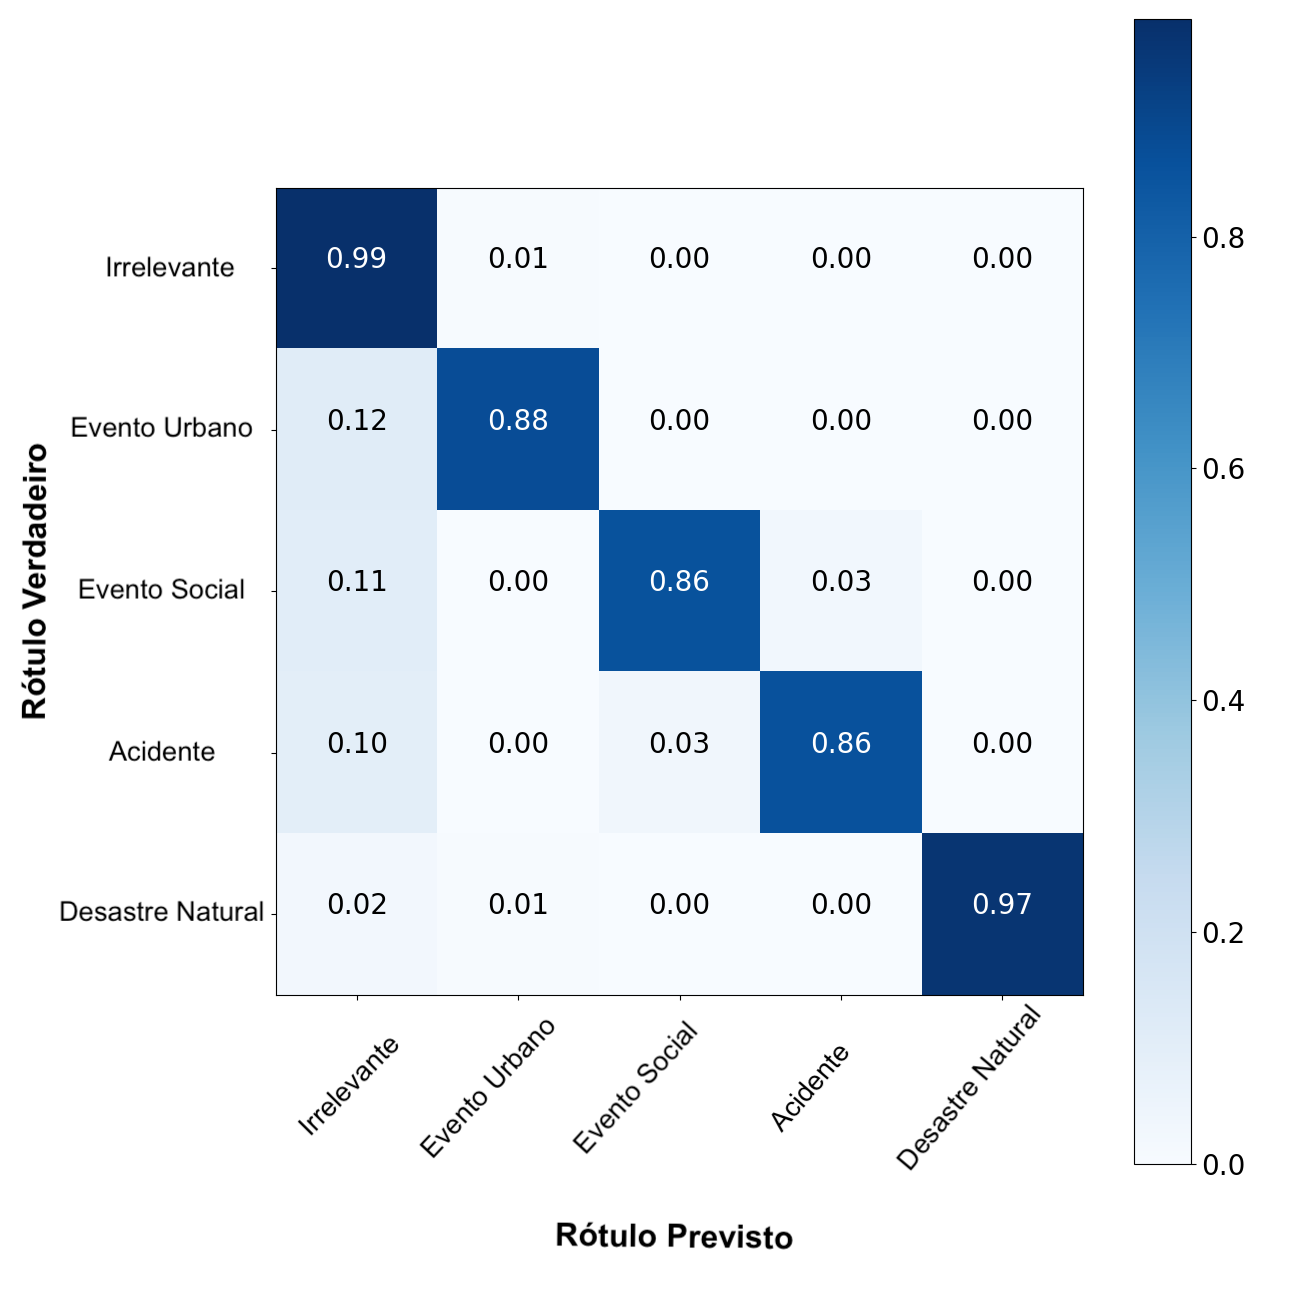
\includegraphics[width=1\linewidth]{images/confusion_matrix_mlp_pt.png}
	\label{fig:confusion_matrix_mlp}
	\source{Felipe Cordeiro Alves Dias (2019)}
\end{figure}

Dos 60.984 \textit{tweets}, 10.027 foram classificados manualmente em eventos de exceção e desse subconjunto foram encontrados 8.112 endereços, como pode ser visto na Tabela~\ref{tab:qtdExtractedAddresses} --- desconsiderando o tipo de localidade \textit{APPROXIMATE} (explicado mais adiante) --- (o que representa 80,90\% do total dos \textit{tweets} classificados como eventos de exceção, sem considerar a classe Irrelevante). A quantidade de endereços extraídos por classe está descrita na Tabela~\ref{tab:qtdExtractedAddresses}, as razões para \textit {tweets} sem endereço extraído são:

\begin{enumerate*}
\item \textit{Tweets} apenas com o ponto de interesse, ou seja, não consta explicitamente o endereço.
\item \textit{Tweets} sem informação de endereço.
\item \textit{Tweets} com nome de logradouro incomum (por exemplo \emph{passagem}, \emph{complexo viário}, \emph{ligação sentido}).
\item \textit{Tweets} com endereços com palavras concatenadas (por exemplo \emph{avenidapaulista}).
\end{enumerate*}

Os \textit{tipos de localidades}\footnote{Disponível em \url{https://developers.google.com/maps/documentation/geocoding}. Acesso em 16 de setembro de 2018.} são classificados pela \textit{Google Geocoding API} em:
\begin{enumerate*}
\item \textit{ROOFTOP} --- Indica que o resultado retornado há informações de localização com precisão a nível do endereço de rua.
\item \textit{RANGE\_INTERPOLATED} --- Indica que o resultado retornado reflete uma aproximação interpolada entre dois pontos precisos (como interseções). Geralmente, os resultados interpolados são retornados quando os códigos geográficos do \textit{rooftop} não estão disponíveis para um endereço de rua.
\item \textit{GEOMETRIC\_CENTER} --- Indica que o resultado retornado é o centro geométrico de um resultado.
\item \textit{APPROXIMATE} --- Indica que o resultado retornado é aproximado.
\end{enumerate*}

Neste estudo de caso, desconsideramos os endereços com classificação \textit{APPROXIMATE}, devido ao fato de poderem comprometer a confiabilidade das análises realizadas. 

\begin{table}[!htb]
\centering
\caption {Quantidade\tnote{f} de endereços extraídos por classe}
\label {tab:qtdExtractedAddresses}
\begin{threeparttable}
\begin{tabular}{c|c|c|c|c|c}
\toprule
\textbf{Classe} & \textbf{\#endereços extraídos\tnote{a}} & \textbf{\textit{\#APP\tnote{b}}} & \textbf{\textit{\#GEO\tnote{c}}} & \textbf{\textit{\#RANGE\tnote{d}}} & \textbf{\textit{\#ROOF\tnote{e}}} \\
\midrule
Acidente & 3.439 & 7 & 805 & 1.130 & 1.497 \\
\hline
Irrelevante & 451 & 13 & 292 & 6 & 140 \\
\hline
Desastre Natural & 2.464 & 9 & 340 & 719 & 1.396 \\
\hline
Evento Social & 793 & 4 & 761 & 2 & 26 \\
\hline
Evento Urbano & 1.002 & 4 & 942 & 10 & 46 \\
\midrule
\midrule
\textbf{Total} & 8.149 & 37 & 3.140 & 1.867 & 3.105 \\
\bottomrule
\end{tabular}
\begin{tablenotes}
\item[a] Total de endereços extraídos
\item[b] Total de endereços extraídos com o tipo de localidade \textit{APPROXIMATE}
\item[c] Total de endereços extraídos com o tipo de localidade \textit{GEOMETRIC\_CENTER}
\item[d] Total de endereços extraídos com o tipo de localidade \textit{RANGE\_INTERPOLATED}
\item[e] Total de endereços extraídos com o tipo de localidade \textit{ROOFTOP}
\item[f] Total considerando endereços repetidos, a repetição é importante para identificarmos os endereços mais impactados por eventos de exceção.
\end{tablenotes}
\end{threeparttable}
\source{Felipe Cordeiro Alves Dias (2019)}
\end{table}


A Figura~\ref{fig:address_analysis} mostra os endereços\footnote{Lista completa está disponível em \url{https://docs.google.com/spreadsheets/d/1gn1cTDifUJEPdgcU67SC45GdYHRKmIHtAfJwRBm088s/edit?usp=sharing}. Acesso em 09 de setembro de 2018.} detectados que foram mais afetados por eventos de exceção e a Figura~\ref{fig:dispersion} mostra parte da distribuição desses eventos na região central da cidade de São Paulo. É importante ressaltar que os eventos de exceção relacionados a eventos sociais estão concentrados em maioria em endereços popularmente conhecidos (grande parte das manifestações acontecem na Av. Paulista, por exemplo), o que é um indício visual de que a metodologia é adequada.

\begin{figure}[!htb]
	\centering
 	  \caption{Endereços mais impactados por eventos de exceção}
		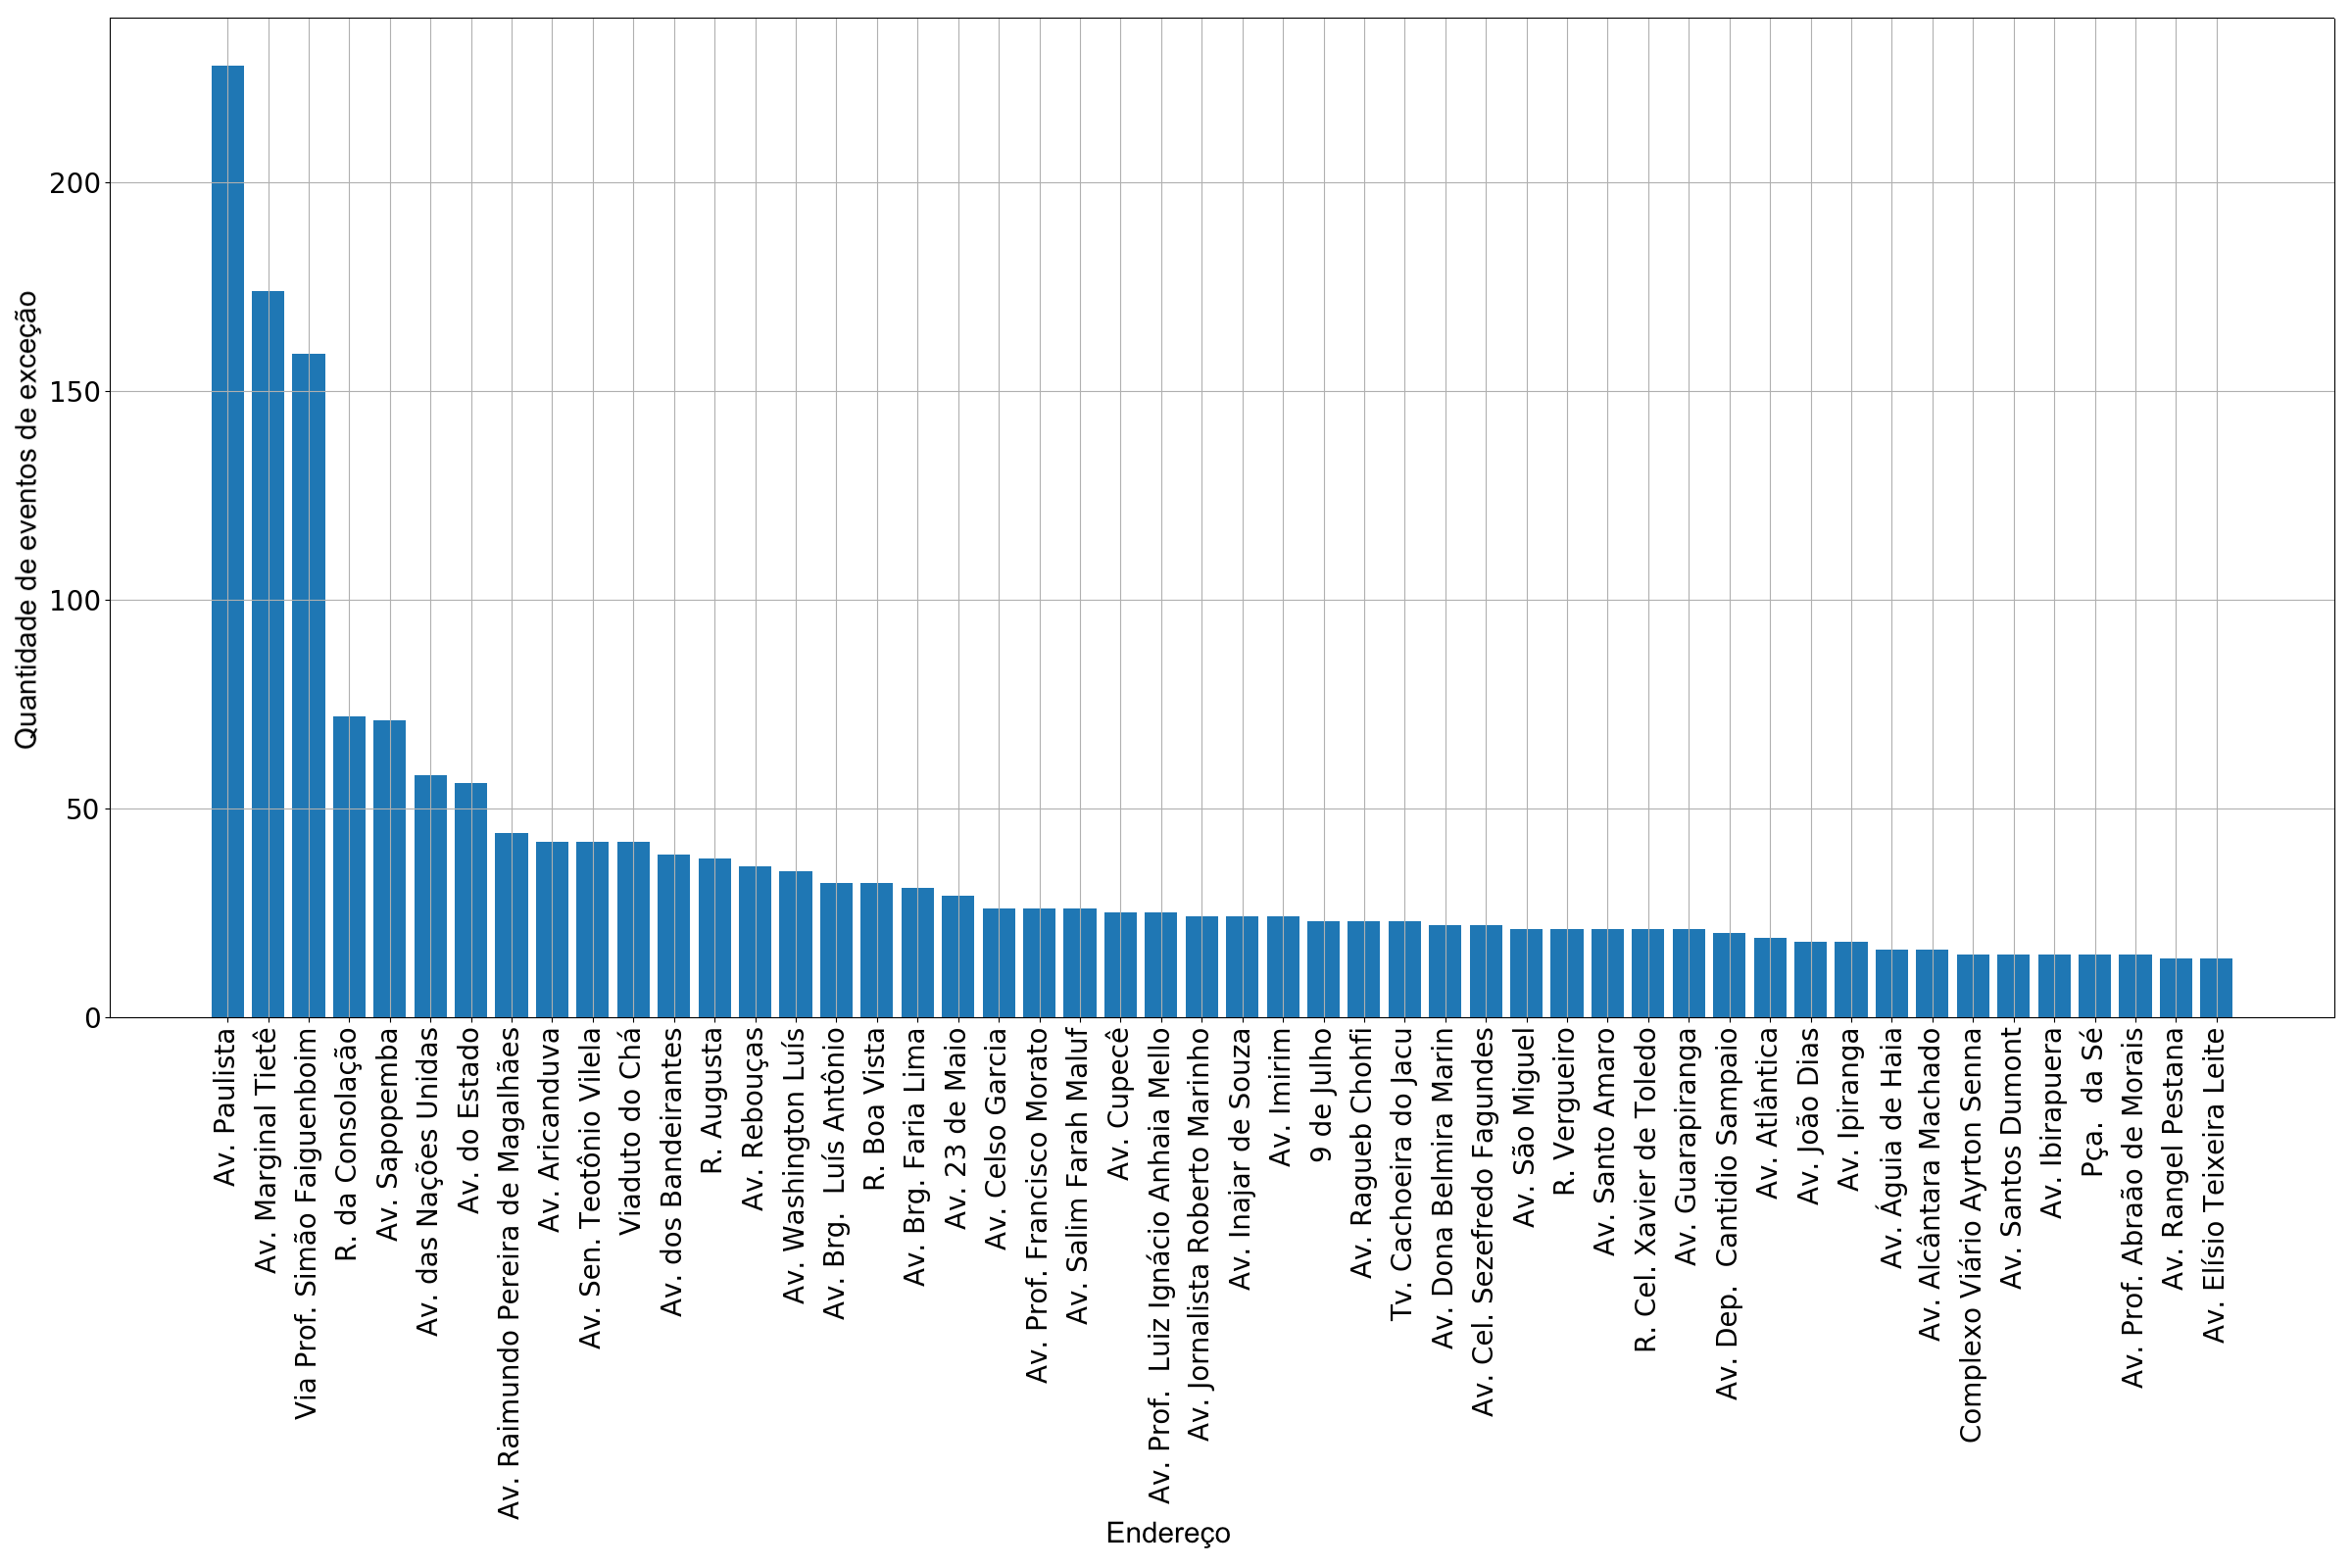
\includegraphics[width=1\linewidth]{images/address_analysis_pt.png}
	\label{fig:address_analysis}
	\source{Felipe Cordeiro Alves Dias (2019)}
\end{figure}

\begin{figure}[!htb]
	\centering
 	  \caption{Distribuição dos eventos de exceção na região central de São Paulo}
		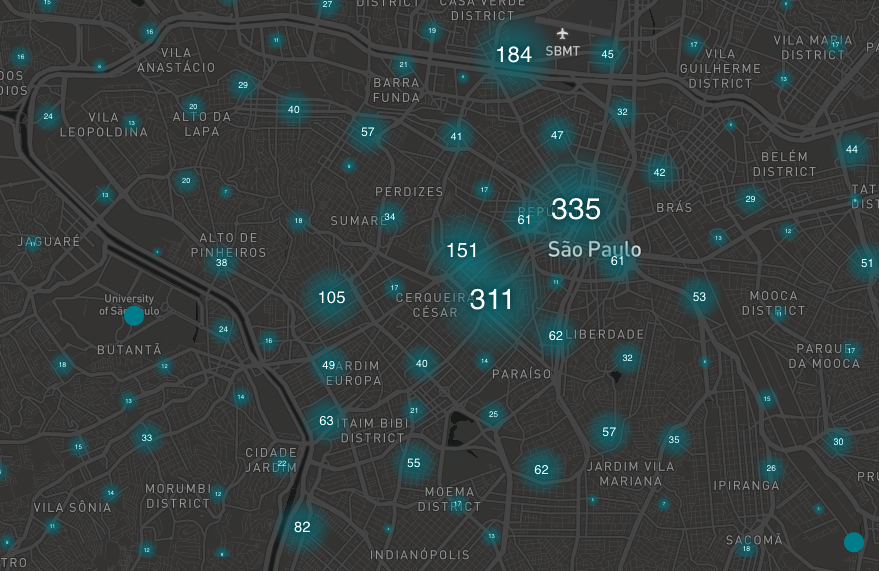
\includegraphics[width=1\linewidth]{images/exception_events_sp.png}
	\label{fig:dispersion}
	\source{Felipe Cordeiro Alves Dias (2019)}
\end{figure}

Consideramos que uma linha de ônibus é afetada por um evento de exceção se uma \textit{stop} estiver dentro de um raio de 1000 metros de distância do evento. Utilizando este critério, o total de 992 linhas de ônibus foram afetadas por eventos de exceção durante este período, sendo ``33389'' o código da linha de ônibus mais impactada. Essa linha específica foi impactada por 1.301 eventos de exceção. A Tabela~\ref{tab:impacted_bus_code_lines} lista as linhas de ônibus que foram impactadas por mais de 600 eventos de exceção.

\begin {table} [!htb]
\centering
\resizebox{16cm}{!}{
\begin{threeparttable}
\caption {Linhas de ônibus mais impactadas por eventos de exceção\tnote{a}}
\label {tab:impacted_bus_code_lines}
\begin {tabular} {c|c|c}
 \toprule
\textbf{Código da linha} & \textbf{\# eventos de exceção} & \textbf{Letreiro} \\
    \midrule
    33389 & 1301  & TERM. PINHEIROS / METRÔ TUCURUVI  \\
\hline

    33284 & 1176  & ITAIM BIBI / METRÔ SANTANA  \\
\hline

    33121 & 1023  & TERM. PRINC. ISABEL / TERM. STO. AMARO  \\
\hline

    32805 & 1006  & TERM. PRINC. ISABEL / CHÁC. SANTANA  \\
\hline

    33112 & 933   & TERM. PQ. D. PEDRO II / JD. SÃO SAVÉRIO  \\
\hline

    33111 & 857   & TERM. AMARAL GURGEL / JD. DA SAÚDE  \\
\hline

    35229 & 841   & TURISMO / CIRCULAR  \\
\hline

    33443 & 816   & ANA ROSA / METRÔ SANTANA  \\
\hline

    32897 & 805   & LUZ / TERM. A. E. CARVALHO  \\
\hline

    35072 & 767   & METRÔ BARRA FUNDA / CONEXÃO PETRÔNIO PORTELA  \\
\hline

    32772 & 759   & TERM. PRINC. ISABEL / TERM. STO. AMARO  \\
\hline

    33253 & 754   & METRÔ BELÉM / JD. BONFIGLIOLI  \\
\hline

    33391 & 748   & METRÔ JABAQUARA / METRÔ SANTANA  \\
\hline

    32813 & 746   & PÇA. DA SÉ / CHÁC. SANTANA  \\
\hline

    32829 & 746   & TERM. BANDEIRA / TERM. CAPELINHA  \\
\hline

    34048 & 719   & LGO. SÃO FRANCISCO / JD. SELMA  \\
\hline

    33486 & 715   & TERM. PQ. D. PEDRO II / TERM. SÃO MATEUS  \\
\hline

    33236 & 708   & TERM. BANDEIRA / JD. JAQUELINE  \\
\hline

    33336 & 697   & PINHEIROS / IMIRIM  \\
\hline

    32816 & 693   & TERM. PQ. D. PEDRO II / TERM. STO. AMARO  \\
\hline

    33534 & 690   & CARDOSO DE ALMEIDA / MACHADO DE ASSIS  \\
\hline

    32838 & 647   & PÇA. DA SÉ / PQ. RES. COCAIA  \\
\hline

    33398 & 639   & CID. UNIVERSITÁRIA / METRÔ SANTANA  \\
\hline

    32769 & 638   & LGO. SÃO FRANCISCO / TERM. CAPELINHA  \\
\hline

    33114 & 637   & TERM. PINHEIROS / SACOMÃ  \\
\hline

    34210 & 637   & LGO. SÃO FRANCISCO / TERM. VARGINHA  \\
\hline

    33116 & 625   & RIO PEQUENO / IPIRANGA  \\
\hline

    33126 & 614   & TERM. BANDEIRA / INOCOOP CAMPO LIMPO  \\
\bottomrule
\end{tabular}
\begin{tablenotes}
            \item[a] Tabela completa no Apêndice~\ref{apendiceD}.
        \end{tablenotes}
\end{threeparttable}
}
\source{Felipe Cordeiro Alves Dias (2019)}
\end{table}

\section{Considerações finais sobre a metodologia desenvolvida}

Este experimento apresenta uma nova metodologia para classificação de eventos de exceção e analisa seus respectivos impactos no sistema de transporte coletivo por ônibus da cidade de São Paulo. De acordo com os experimentos realizados, o algoritmo com maior  acurácia para classificação de \textit{tweets} em eventos de exceção foi \textit{Multi-layer Perceptron}. Também, mostramos que é possível extrair endereços de \textit{tweets} semi-estruturados usando apenas expressões regulares. A classificação desses eventos é o primeiro passo para entender melhor como os eventos de exceção afetam a rede de transporte público.

Embora o método tenha sido validado usando perfis selecionados do Twitter escritos em português brasileiro, o mesmo pode ser generalizado para diferentes idiomas e cidades. A GTFS é um formato ubíquo para o transporte público e ferramentas como a NLTK suporta vários idiomas.

%\subsection{Future work}
%As future work, the methodology presented in this paper will be applied to the other accounts from the Corpus Twitter, described in the Section~~\ref{corpusTwitter}. Besides, we will extract features from the dataset of bus movements, for each bus line affected by the exception events, also we will extract more exception events from another dataset related to reclamations made by bus users to enrich the impact analysis.

%\chapter{Proposta de pesquisa}
%\label{proposta}
%Neste Capítulo, são apresentadas as seções referentes a proposta de pesquisa para a dissertação. Assim, abordaremos a formalização do problema; solução proposta; construção do conjunto de dados; exploração e visualização do conjunto de dados; identificação dos eventos de exceção; correlação dos eventos de exceção com os dados AVL da SPTrans e, por fim, o plano de trabalho.

%\section{Formalização do problema}
%\label{problemForm}

%O problema de caracterização de eventos de exceção e de seus respectivos impactos envolve a fase conhecida como \textit{feature extraction}, do ciclo iterativo do processo de \textit{feature engineering}. \textit{Feature extraction} consiste na extração de um conjunto de características ${\alpha =}$ $\lbrace {\chi_1}, {\chi_2}, ..., {\chi_n} \rbrace$ a partir de um dado de entrada $\chi$. Sendo assim, nessa proposta de pesquisa pretendemos extrair o conjunto de características (utilizando o Corpus \textit{Twitter}) ${E = }$ $\lbrace {\varepsilon_1}, {\varepsilon_2}, ..., {\varepsilon_n} \rbrace$, referente a cada evento de exceção, e o conjunto ${I_{\varepsilon_i} = }$ $\lbrace {\iota_{1\varepsilon_i}}, {\iota_{2\varepsilon_i}}, ..., {\iota_{n\varepsilon_i}} \rbrace$, contendo as características de cada impacto (utilizando o Corpus SPTrans) decorrente de um determinado evento de exceção $\varepsilon_i \in E$.

%Posto que os conjuntos \textit{E} e \textit{I} existem,  tem-se também como problema a correlação de cada evento de exceção com o seu respectivo impacto, permitindo assim uma análise histórica para identificação de padrões de causa e consequência. Tal correlação pode ser definida por uma função sobrejetora, representada formalmente em lógica de primeira ordem pela expressão:
%\begin{equation*} 
%\forall \iota \in I, \exists \varepsilon \in E (\iota = f(\varepsilon) ) 
%\end{equation*}

%Dessa forma, para todo impacto $\iota$ pertencente ao conjunto \textit{I} existe um evento de exceção $\varepsilon_i$ pertencente ao conjunto \textit{E}. 

%\section{Solução proposta}
%\label{solutionProp}

%A solução proposta pretende coletar \textit{tweets} dos \textit{profiles} contidos na tabela~\ref{tab:oficialProfiles}, pré-processá-los, extrair e selecionar \textit{features} para serem utilizadas em algoritmos de classificação, obtendo dessa forma os eventos de exceção. 
%Com esses eventos de exceção pretendemos analisar a base histórica da SPTrans de dados AVL (transmitidos utilizando AVL), e identificar os possíveis impactos de cada evento de exceção. O processo de identificação dos impactos contidos na base histórica da SPTrans pode ser definido com base nas localizações extraídas dos \textit{tweets} coletados e posteriormente geolocalizadas. 

%As localizações dos \textit{tweets} podem ser extraídas usando a seguinte fórmula em expressão regular: 
%\begin{equation}
%ER = \lbrace L_1|S_1|L_2|S_2|...|L_n|S_n \rbrace \lbrace [a-zA-Z \backslash s]+ \rbrace
%\end{equation}
%Tal expressão regular é dividida em dois conjuntos, no primeiro ($\lbrace L_1|S_1|L_2|S_2|...|L_n\\|S_n \rbrace$), os logradouros (L) e siglas (S) contidas na tabela~\ref{tab:logradouros} (no apêndice~\ref{apendiceB}) são concatenadas, especificando um filtro para identificar cadeias de caracteres iniciadas com um logradouro ou sigla. No segundo conjunto ($\lbrace [a-zA-Z \backslash s]+ \rbrace$), o filtro especificado identifica as palavras seguintes aos logradouros e siglas.

%Em resumo, propomos solucionar o problema de caracterização dos eventos de exceção e de seus respectivos impactos seguindo os seguintes passos: (I) coleta de \textit{tweets} de órgãos responsáveis por notificar eventos de exceção; (II) identificação dos \textit{tweets} relacionados a eventos de exceção; (III) extração e geolocalização dos endereços dos eventos de exceção e (IV) análise e correlação com os dados AVL.

%\subsection{Algoritmos de Aprendizado de Máquina}

%Após a extração e seleção de \textit{features}, planejamos classificar manualmente 30\% dos \textit{tweets} com base em suas respectivas \textit{features}, utilizando-os como conjunto de teste. Posteriormente, pretendemos analisar os algoritmos de aprendizado de máquina elencados pela revisão sistemática em~\ref{iaClassification} para escolhermos dentre eles o com maior acurácia para identificar eventos de exceção, por meio de classificação.

%\section{Plano de trabalho}
%\label{workPlan}

%Nesta seção, são apresentados o cronograma (tabela~\ref{tab:schedule}) e as atividades realizadas e planejadas para o desenvolvimento do projeto referente a proposta de pesquisa, enumeradas a seguir:

%\begin{enumerate}
%\item Revisão Bibliográfica.
%\begin{enumerate}
%\item Revisão Sistemática sobre estudos de caso utilizando \textit{tweets} na caracterização de problemas urbanos e relacionados ao transporte público.
%\end{enumerate}
%\item Desenvolvimento de protótipo.
%\begin{enumerate}
%\item Serviço para coleta, processamento e armazenamento de \textit{tweets} dos \textit{profiles} selecionados contidos na tabela~\ref{tab:oficialProfiles}.
%\item Extração e geolocalização dos endereços contidos nos \textit{tweets}.
%\item Implementação de \textit{scripts} para extração, transformação e armazenamento dos dados AVL da SPTrans.
%\item Implementação de \textit{scripts} para extração, transformação e armazenamento dos dados da GTFS da SPTrans.
%\item Criação de especificações de ingestão de dados para os dados AVL da SPTrans e dos \textit{tweets} dos \textit{profiles} selecionados contidos na tabela~\ref{tab:oficialProfiles} para o banco de dados de séries temporais \textit{Druid}\footnote{\label{druidIo}\url{http://druid.io}. Acesso em 29 de outubro de 2017.}.
%\item Integração da ferramenta \textit{Superset}\footnote{\label{superset}\url{http://superset.apache.org}. Acesso em 29 de outubro de 2017.} com o \textit{Druid}\footref{druidIo} para exploração e visualização dos dados AVL da SPTrans e dos \textit{tweets} dos \textit{profiles} selecionados contidos na tabela~\ref{tab:oficialProfiles}.
%\item Implementação de \textit{scripts} para automação dos processos de ingestão de dados e \textit{deploy} e monitoramento dos serviços do \textit{Druid}\footref{druidIo} e Superset\footref{superset}.
%\item Configuração do ambiente em nuvem para execução do \textit{Druid}\footref{druidIo} e \textit{Superset}\footref{superset}.

%\end{enumerate}
%\item Construção do conjunto de dados.
%\begin{enumerate}
%\item Obtenção dos dados AVL de janeiro a dezembro de 2016 e de janeiro a setembro de 2017, de todas as linhas de ônibus de São Paulo.
%\item Obtenção da base de dados dos últimos cinco anos das reclamações relacionadas a SPTrans, realizadas na Central de Atendimento ao Cidadão (156) da Prefeitura de São Paulo.
%\item Obtenção de um conjunto de \textit{tweets} dos \textit{profiles} selecionados contidos na tabela~\ref{tab:oficialProfiles}.
%\end{enumerate}
%\item Implementação da solução proposta.
%\begin{enumerate}
%\item Identificação dos eventos de exceção (pré-processamento, \textit{feature extraction} e \textit{feature selection} dos \textit{tweets} coletados).
%\item Estudo dos algoritmos de classificação e implementação de um artefato de \textit{software} para classificação dos \textit{tweets} de acordo com seus respectivos eventos de exceção.
%\item Correlação dos eventos de exceção com os dados AVL da SPTrans.
%\end{enumerate}
%\item Avaliação dos resultados parciais obtidos durante e após o desenvolvimento da solução proposta.
%\item Escrita de artigo para submissão em periódicos ou eventos da área.
%\item Escrita da dissertação.
%\end{enumerate}

%\begin{table}[!htb]
%  \centering
%  \caption{Cronograma de atividades}
%  \resizebox{\textwidth}{!}{%
%    \begin{tabular}{cccccccccccccccccccc} \hline
%    \multicolumn{2}{c}{Atividade } & \multicolumn{12}{c}{2017}                                                                     & \multicolumn{6}{c}{2018} \\ 
%    Número & Descrição & 1     & 2     & 3     & 4     & 5     & 6     & 7     & 8     & 9     & 10    & 11    & 12    & 1     & 2     & 3     & 4     & 5     & 6 \\ \hline
%    1     & Revisão bibliográfica & X     & X     & X     & X     & X     & X     &       &       &       &       &       &       &       &       &       &       &       &  \\
%    2     & Desenvolvimento de protótipo &       &       & X     & X     & X     & X     &       &       &       &       &       &       &       &       &       &       &       &  \\
%    3     & Construção do conjunto de dados &       &       &       &       &       &       & X     & X     & X     & X     & X     &       &       &       &       &       &       &  \\
%    4     & Implementação da solução proposta &       &       &       &       &       &       &     &      &      &      &      & X     &   X    &  X     &   X    &  X   &   X   &  \\
%    5     & Avaliação dos resultados &       &       &       &       &       &       &       &       &       &      &     &      &   X    &       &   X    &       &   X    &  \\
%    6    & Escrita de artigo &       &       &       &       &       &       &       &       &       &       &      &       &       &   X    &   X    &       &       &  \\ 
%    7     & Escrita da dissertação &       &       & X     & X     & X     & X     & X     & X     & X     & X     & X     & X     & X     & X     & X     & X     & X     & X \\
%    \hline
%    \end{tabular}%
%    }
%  \label{tab:schedule}%
% \source{Felipe Cordeiro Alves Dias, 2017}
%\end{table}%

\chapter{Caracterização do impacto dos eventos de exceção}
\label{dataCorr}

As seções deste capítulo são referentes aos experimentos para caracterização dos impactos em relação às velocidades medianas dos ônibus e identificação dos padrões de velocidade média dos dados AVL. Decidimos por realizar os experimentos com velocidade mediana e média para analisarmos se há divergências entre os dois estudos, devido a possíveis discrepâncias nos valores das velocidades instantâneas, seja por questões climáticas ou limitações dos módulos AVL.

\section{Caracterização dos impactos em relação às velocidades medianas dos ônibus}
\label{dataCorr2}

Dado que os eventos de exceção podem ser identificados utilizando \textit{tweets} dos perfis contidos na Tabela~\ref{tab:oficialProfiles}, há também a possibilidade de caracterizarmos seus respectivos impactos em relação às velocidades medianas dos ônibus, por meio da base histórica dos dados AVL da SPTrans.  Neste estudo consideramos os eventos de exceção geolocalizados do ano de 2017 do \textit{Corpus Twitter}, classificados manualmente. A distribuição desses eventos ao longo dos meses pode ser observada  na Figura~\ref{fig:geolocated_exception_events_distribution}, assim como de suas respectivas classes na Figura~\ref{fig:exception_events_classification_distribution}.

%Dito isso, inicialmente pretendemos caracterizar os impactos em:

%\begin{itemize}
%\item Atraso médio induzido nas viagens.
%\item Ônibus frequentemente afetados por eventos de exceção.
%\item Ônibus frequentemente afetados por determinado evento de exceção.
%\item Padrão de ocorrência dos eventos de exceção no espaço-tempo (localizações e \textit{timestamps}).
%\item Quantidade e viagens afetadas.
%\item Quantidade e regiões da cidade de São Paulo afetadas.
%\item Viagens frequentemente afetadas por eventos de exceção.
%\item Viagens frequentemente afetadas por determinado evento de exceção.
%\end{itemize}

\begin{figure}[!htb]
	\centering
 	  \caption{Distribuição do número de eventos de exceção geolocalizados}
		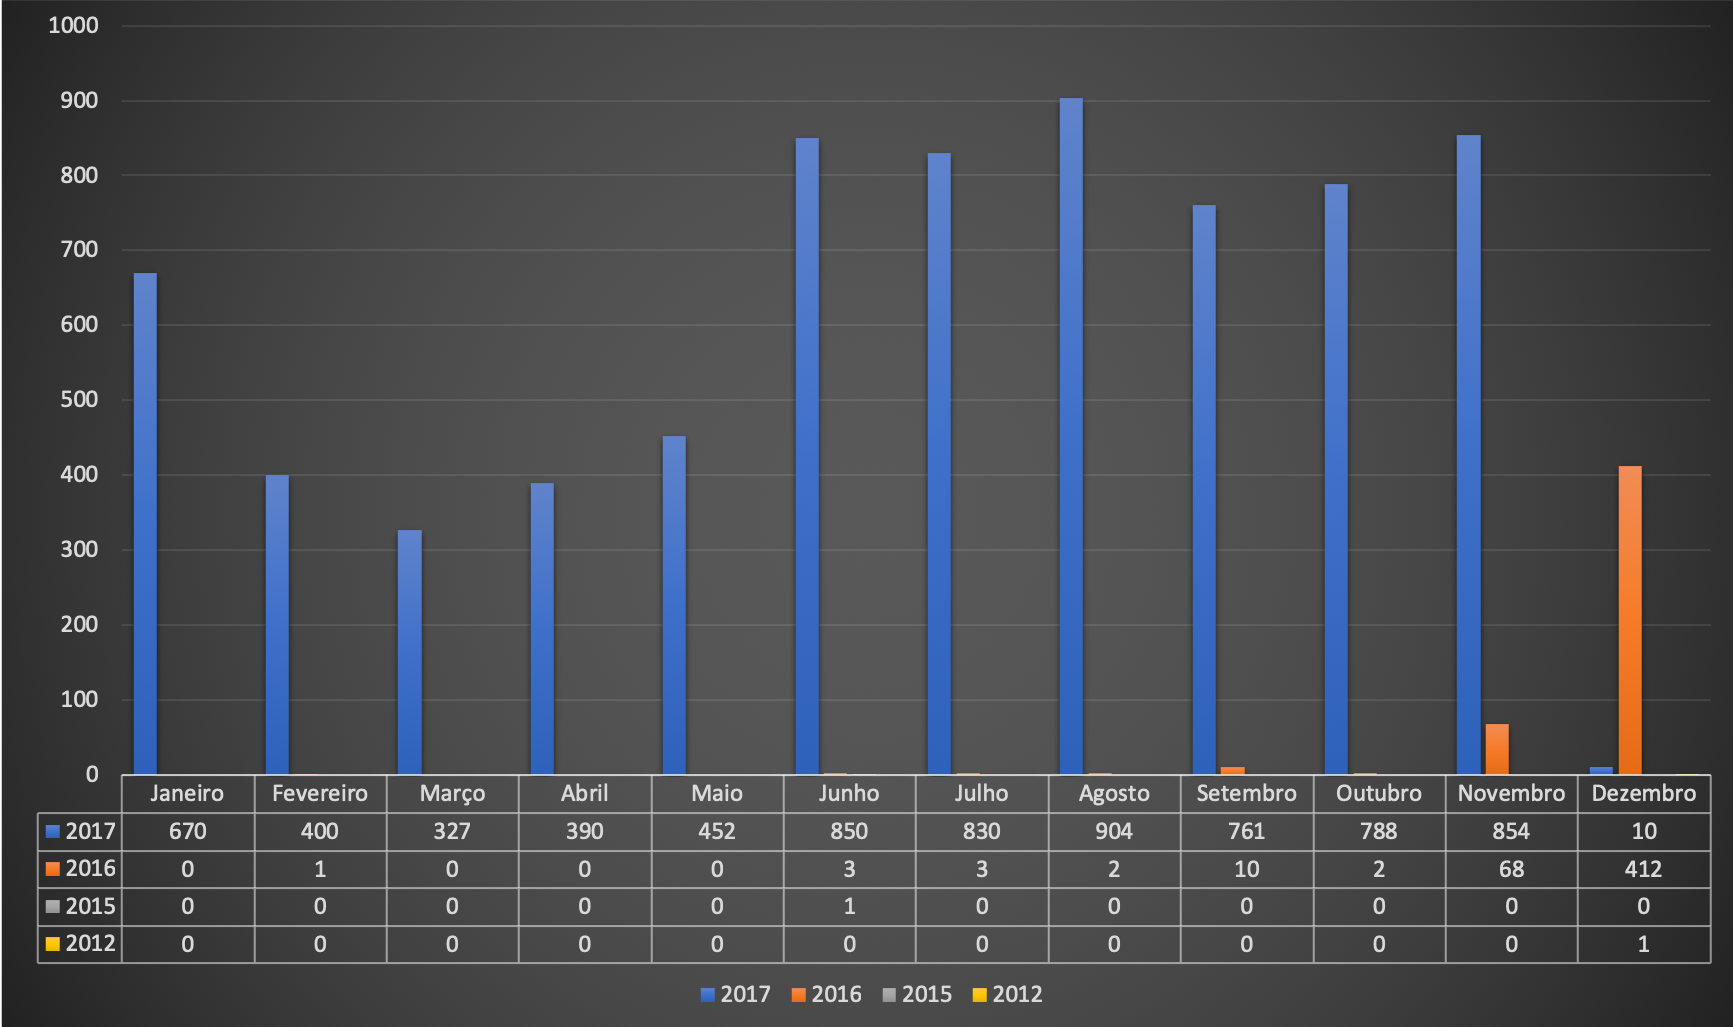
\includegraphics[width=1\linewidth]{images/geolocated_exception_events_distribution_pt.png}
	\label{fig:geolocated_exception_events_distribution}
	\source{Felipe Cordeiro Alves Dias (2019)}
\end{figure}

Conforme descrito no Capítulo~\ref{exp1} e ilustrado na Figura~\ref{fig:avl_tweets_correlation_pt}, identificamos as linhas afetadas por eventos de exceção filtrando as paradas de ônibus (contidas na coleção \textit{stops}  e \textit{shapes} da GTFS da SPTrans) dentro de um raio de 1.000 metros das geolocalizações extraídas dos \textit{tweets}. No processo de caracterização do impacto consideramos as distâncias de 100 m e 1.000 m, pois o impacto pode ser diferente de acordo com a proximidade ao evento. No entanto, para encontrarmos um número significativo de linhas impactadas consideramos apenas a distância de 1.000 m.

A partir disso, selecionamos os dados de movimentação que serão analisados. Considerando a sazonalidade dos dias da semana, selecionamos para análise apenas os dias da semana pertencentes ao mês de ocorrência do evento e com nomes iguais ao nome do dia da semana no qual o evento de exceção aconteceu. Isso porque os dias da semana possuem padrões diferentes de movimentação. Por exemplo, às sextas-feiras ocorrem inúmeros eventos sociais que normalmente acarretam em um trânsito mais congestionado. Os dias da semana são restritos ao mês de ocorrência do evento devido ao fato de que os meses também são afetados pela sazonalidade --- festas no final do ano, férias, início de períodos letivos, etc. --- conforme Figura~\ref{fig:exception_events_classification_distribution}.

\begin{figure}[!htb]
	\centering
 	  \caption{Distribuição das classes de eventos de exceção geolocalizados ao longo dos meses do ano de 2017}
		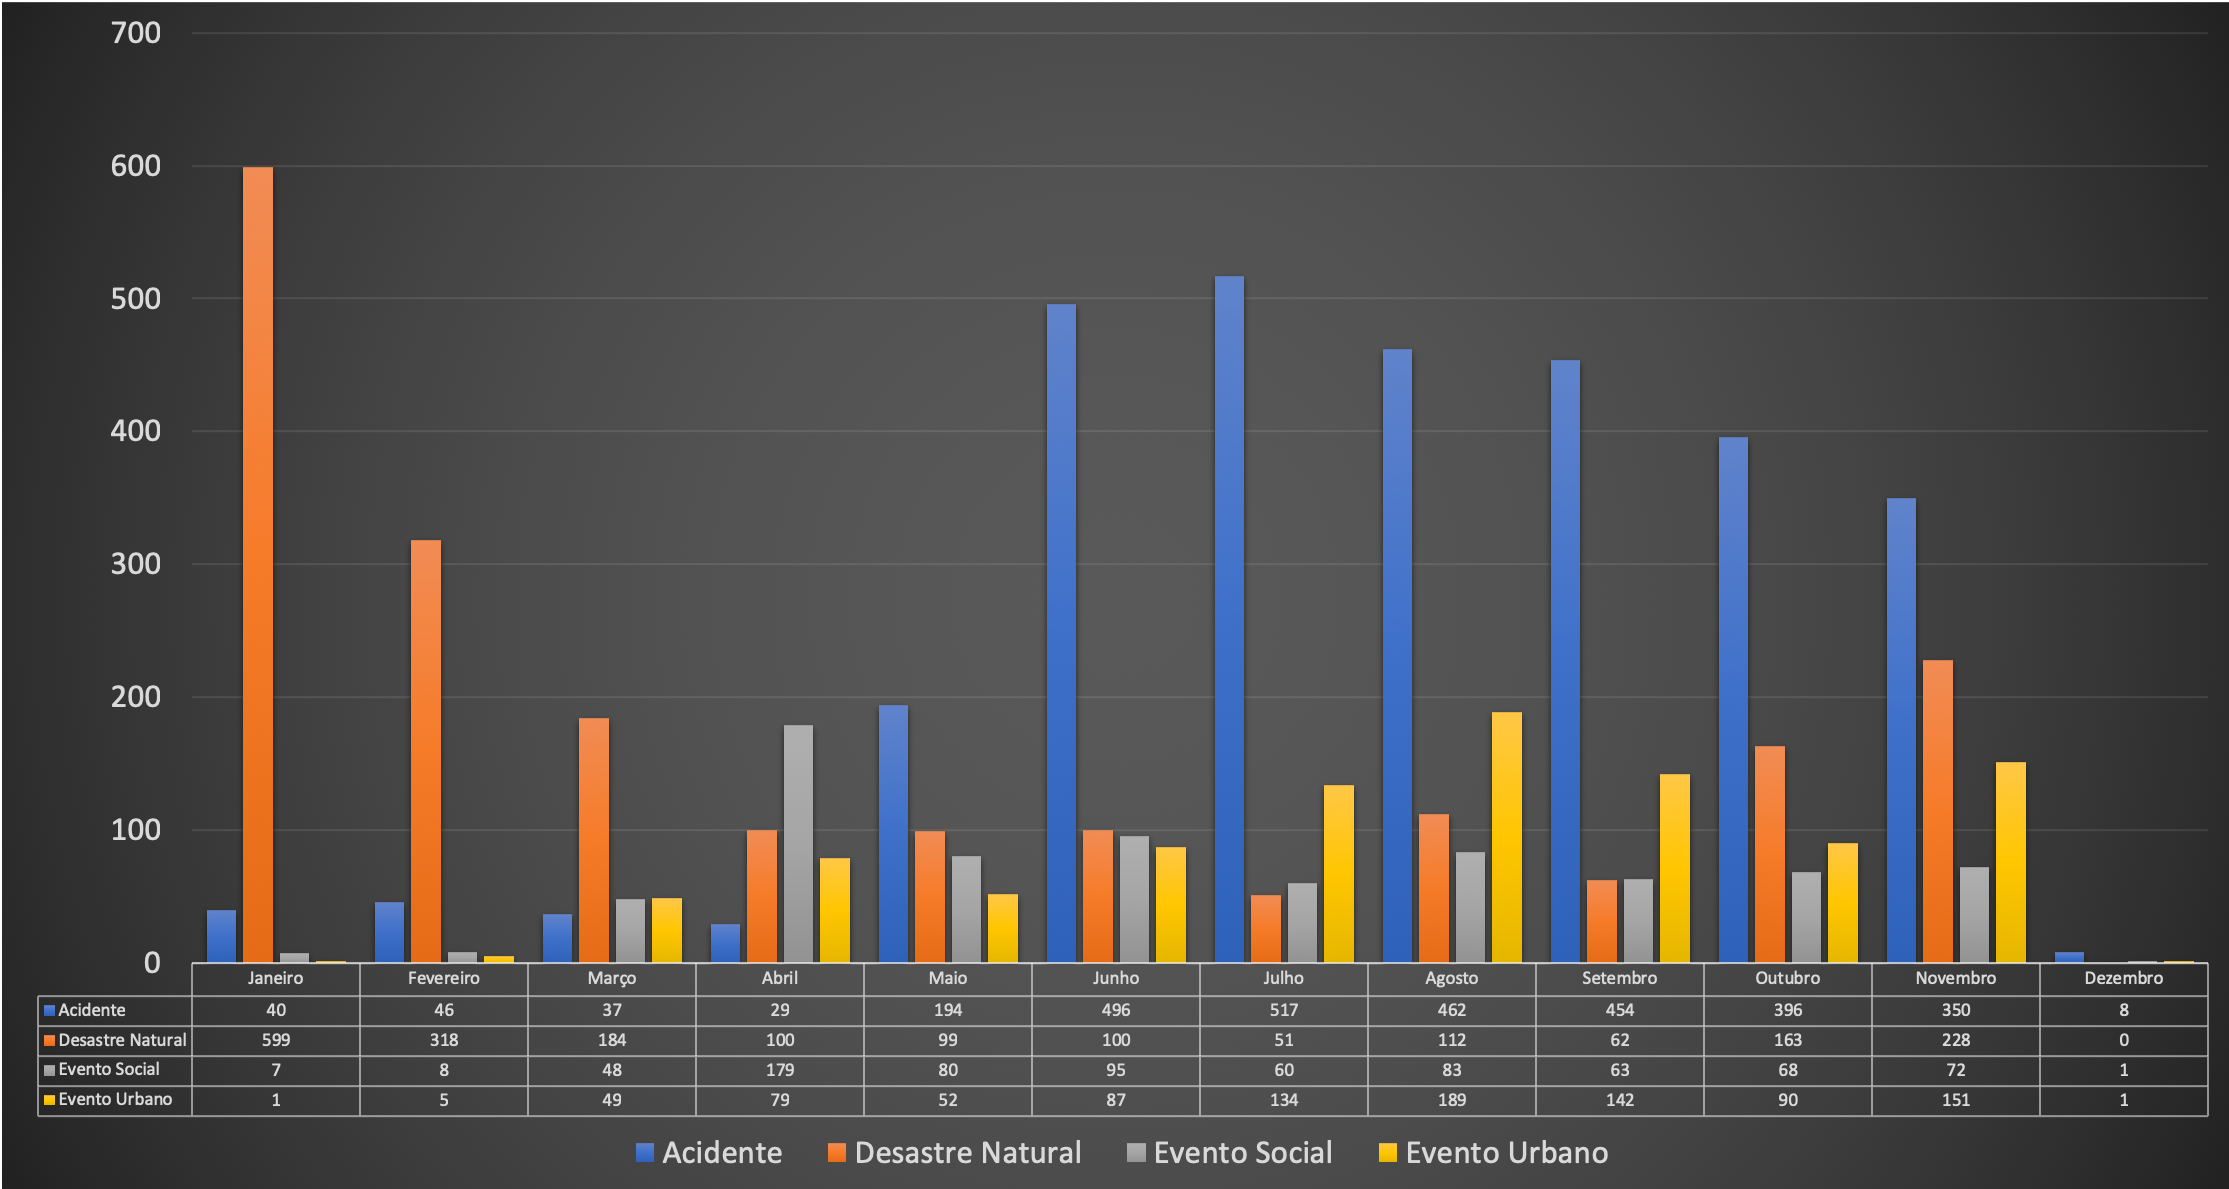
\includegraphics[width=1\linewidth]{images/exception_events_classification_distribution_pt.png}
	\label{fig:exception_events_classification_distribution}
	\source{Felipe Cordeiro Alves Dias (2019)}
\end{figure}

\begin{figure}[!htb]
	\centering
 	  \caption{Processo para correlação entre os dados AVL, GTFS e \textit{tweets} para análise do impacto dos eventos de exceção}
		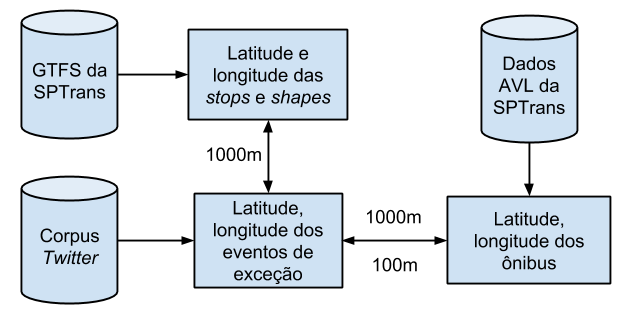
\includegraphics[width=0.7\linewidth]{images/avl_tweets_correlation_pt.png}
	\label{fig:avl_tweets_correlation_pt}
	\source{Felipe Cordeiro Alves Dias (2019)}
\end{figure}

Além dos filtros referentes a sazonalidades dos dias da semana e meses, também filtramos os dados relacionados às linhas impactadas a um raio de distância de 100 e de 1.000 metros do evento de exceção em questão, além de considerarmos a mesma faixa de horário do \textit{tweet}. Por exemplo, se o horário do \textit{tweet} é às 17h15min, consideramos os dados AVL com horário entre 17h e 18h. É importante observar que esse trabalho não considera o início e término exato dos eventos de exceção, mas uma faixa de horário de uma hora a partir do hora contida no \textit{timestamp}  do \textit{tweet}.

Em seguida, agregamos os dados selecionados para analisarmos  de forma descritiva a velocidade instantânea de cada linha de ônibus. Com isso, extraímos dados sobre a velocidade máxima, mínima, média, mediana, variância, desvio padrão e porcentagem de dados com velocidades iguais e diferentes de zero. 

Após isso, comparamos por meio da Equação \ref{eqVeloc} se a velocidade mediana do dia do evento de exceção é uma velocidade esperada, com base nas velocidades medianas do demais dias da semana.  Consideramos que a linha foi impactada se o valor retornado da função abaixo for 1 e, 0 caso contrário. Com base nisso, consideramos que o conjunto de linhas foi impactado se a quantidade de linhas impactadas for maior ou igual a 50\%.

\begin{equation}
\label{eqVeloc}
 f(n) =
  \begin{cases}
    0      & \quad \text{se  vel.~mediana~do~dia~do~evento} > \frac{\text{vel.~mediana~dos~dias~da~semana}}{\text{total~de~vel.~medianas}}\\
    1 & \quad \text{se vel.~mediana~do~dia~do~evento} \leq \frac{\text{vel.~mediana~dos~dias~da~semana}}{\text{total~de~vel.~medianas}}
  \end{cases}
\end{equation}

\subsection{Resultados}

As seções seguintes são sobre os experimentos relacionados a análise da redução da velocidade mediana dos ônibus a partir das informações de latitude e longitude dos pontos de parada e de rotas.

\subsubsection{Análise da redução da velocidade mediana dos ônibus a partir das informações de latitude e longitude dos pontos de parada}
\label{stopsAnalysis}

Utilizando a metodologia anteriormente descrita, podemos observar na Tabela~\ref{tab:exceptEventVelocityImpAllStop} que os eventos de exceção relacionados a eventos sociais possuem em média 87,04\% de impacto na mediana das velocidades dos grupos de linhas de ônibus afetadas a um raio de 1.000 metros de distância e 100\% a um raio de 100 metros, isso provavelmente devido ao grande número de pessoas envolvidas neste tipo de evento, quantidade de avenidas com fluxo do trânsito modificado ou interrompido.

Os eventos urbanos, por sua vez, impactam em 70,11\% na mediana das velocidades dos grupos de linhas de ônibus afetadas a 1.000 metros e 98,86\% a 100 metros, mesmo sendo realizados com planejamento de rotas alternativas e sinalizações nas vias públicas. A terceira e quarta classes mais afetadas são as de acidentes e desastres naturais, respectivamente, 66,51\% e 59,77\% a 1.000 metros e 98,39\% e 99,80\% a 100 metros, as quais normalmente resultam em bloqueios ou desvios em vias públicas utilizadas pelos ônibus.

Além disso, janeiro, fevereiro e março foram os três meses mais afetados por eventos de exceção relacionados a desastres naturais, período de grandes volumes de precipitação de chuva em São Paulo, no qual normalmente ocorre deslizamentos de terra, quedas de árvores e inundações.  Em relação aos eventos sociais, o ano de 2017 foi marcado com inúmeras manifestações políticas; neste contexto, o mês de maio foi o mais impactado por esse tipo de evento de exceção, principalmente devido aos protestos contra o governo Temer\footnote{{http://www1.folha.uol.com.br/poder/2017/05/1884977-manifestacao-anti-temer-reune-centenas-de-pessoas-na-av-paulista.shtml}. Acesso em 02 de dezembro de 2018}. Os eventos relacionados a acidentes normalmente ocorrem em maior concentração nos períodos de festas e feriados, o que pode ser observado nos meses de janeiro e abril (único mês de 2017 com dois feriados prolongados), com média de impacto de 83,33\% e 87,50\% nas velocidades médias, respectivamente.  Os impactos relacionados a eventos urbanos ocorrem normalmente durante todos os meses, devido a isso são mais uniformes.

Os valores dos meses das tabelas \ref{tab:exceptEventVelocityImpAllStop} e \ref{tab:exceptEventVelocityImpAllShapes} iguais a 100\% de impacto nas velocidades medianas são justificados devido ao pouco volume de eventos para uma determinada classe em um determinado mês, conforme mostra a Figura~\ref{fig:exception_events_classification_distribution}. Analogamente, os meses e classes sem dados de impacto são meses com pouco dados para a classe em questão.

\begin{table}[!htb]
\centering
\caption {Porcentagem de ônibus dos grupos de linhas afetadas por eventos de exceção, a 1.000~m e 100~m de distância, respectivamente, que tiveram a velocidade mediana reduzida nos meses do ano de 2017}
\label{tab:exceptEventVelocityImpAllStop}
\resizebox{16cm}{!}{
\begin{tabular}{c|cc|cc|cc|cc}
\toprule
\textbf{Mês} & \multicolumn{2}{c}{\textbf{Acidente}} & \multicolumn{2}{c}{\textbf{Desastre Natural}} & \multicolumn{2}{c}{\textbf{Evento Social}} &
\multicolumn{2}{c}{\textbf{Evento Urbano}}\\
\cmidrule(l){2-3} \cmidrule(l){4-5} \cmidrule(l){6-7} \cmidrule(l){8-9}
 & 1.000 m & 100 m & 1.000 m & 100 m & 1.000 m & 100 m & 1.000 m & 100 m \\
\midrule
Janeiro & 83,33 &  100 & 
64,23 &  98,00 & 
100 & --- &
 100 & --- \\
\hline
Fevereiro & 70,58 &  100 &
 66,25 &  100 &
 100 & 100 &
 80 & --- \\
\hline
Março &  50,00 &  --- & 
66,66 &  100 &
85,00 & 100 &
68,18 & 100 \\
\hline
Abril & 87,50 &100 & 
 61,11 & 100 & 
 82,75 & 100 & 
 76,92 &  100 \\
\hline
Maio & 65,13 &  100 &
 58,82 &  100 &
 93,33 & 100 &
 50,00 & 100 \\
\hline
Junho & 54,46 &  100 &
 61,53 &  100 &
 76,47 & 100 &
 72,41 & 100 \\
\hline
Julho & 61,48 &  98,41 &
 66,66 & 100 &
 69,23 & 100 &
58,13 & 100 \\
\hline
Agosto & 57,86 & 87,17 &
 55,35 & 100 &
 85,54 & 100 & 
 68,10 & 90,90 \\
\hline
Setembro & 64,21 & 100 &
 42,10 & 100 &
 92,30 & 100 & 
 62,06 & 100 \\
\hline
Outubro & 70,49 & --- &
 56,81 & --- &
 80,00 & --- &
 61,11 & --- \\
\hline
Novembro & 66,66 & 100 &
 57,99 & 100 &
 92,85 & 100 &
 74,35 & 100 \\
\hline
Dezembro & --- & --- & --- & --- & --- & --- & --- & ---  \\
\midrule
\midrule
\textbf{Total} & 66,51 & 98,39 & 59,77 & 99,80 & 87,04 & 100 & 70,11 & 98,86  \\
\bottomrule
\end{tabular}
}
\source{Felipe Cordeiro Alves Dias (2019)}
\end{table}

\subsubsection{Análise da redução da velocidade mediana dos ônibus a partir das informações de latitude e lagitudade das rotas das linhas}

Referente aos dados da Tabela~\ref{tab:exceptEventVelocityImpAllShapes}, para o raio de 1.000~m os eventos que mais reduzem as velocidades medianas são os relacionados a eventos sociais, urbanos, acidentes e desastres naturais, nesta ordem. Apesar disso, é importante observar que o percentual de redução da velocidade mediana, comparado com os da Tabela \ref{tab:exceptEventVelocityImpAllStop}, é reduzido quando consideramos as latitudes e longitudes das rotas como referência para encontrar as linhas impactadas. 

O conjunto de pontos de latitude e longitude utilizados para desenhar as rotas dos ônibus é muito maior do que o que contém as coordenadas espaciais dos pontos de parada, de acordo com a Tabela \ref{tab:gtfs} são 800.767 pontos contra 19.933, respectivamente. Sendo assim, quando as coordenadas das rotas são consideradas como referência para encontrar as linhas afetadas pelos eventos de exceção, obtemos um conjunto maior de linhas impactadas, o que aumenta a margem de erro e o custo computacional. Outra diferença observada é em relação aos percentuais de redução de velocidades medianas para o raio de 100~m. Nesta abordagem, as ordens dos eventos que mais impactam as velocidades medianas são os relacionados a acidentes, desastres naturais, eventos sociais e urbanos, respectivamente.

Em relação às sazonalidades, os meses de  março, abril, maio e outubro foram mais significativos para a redução das velocidades medianas, no raio de de 1.000~m devido as inúmeras manifestações\footnote{\url{https://g1.globo.com/politica/noticia/cidades-pelo-pais-tem-manifestacoes-a-favor-da-lava-jato-neste-domingo.ghtml}. Acesso em 14 de janeiro de 2019.}\footnote{\url{https://g1.globo.com/resumo-do-dia/noticia/quarta-feira-15-de-marco-de-2017.ghtml}. Acesso em 14 de janeiro de 2019.}\footnote{\url{https://www1.folha.uol.com.br/poder/2017/03/1866022-manifestacao-por-intervencao-militar-bloqueia-via-em-sp.shtml}. Acesso em 14 de janeiro de 2019.}\footnote{\url{https://oglobo.globo.com/brasil/ato-de-artistas-no-rio-contra-temer-termina-com-bombas-de-efeito-moral-spray-de-pimenta-21987385}. Acesso em 14 de janeiro de 2019.}\footnote{\url{https://pt.wikipedia.org/wiki/Greve\_geral\_no\_Brasil\_em\_2017}. Acesso em 14 de janeiro de 2019.} que ocorreram no Brasil. Sobre os desastres naturais, os impactos foram relevantes para os meses de janeiro a março, a distância de 100~m, conforme esperado devido ao período de chuvas.

Por fim, a abordagem que utiliza as coordenadas espaciais dos pontos de parada de ônibus como referência pode ser mais adequada do que a que usa os pontos de rota. Isso, devido aos resultados semelhantes obtidos, menor custo computacional e margem de erro.

\begin{table}[!htb]
\centering
\caption {Porcentagem de impacto na velocidade média dos grupos de linhas afetadas por eventos de exceção a 1.000~m e 100~m de distância, respectivamente, nos meses do ano de 2017}
\label{tab:exceptEventVelocityImpAllShapes}
\resizebox{16cm}{!}{
\begin{tabular}{c|cc|cc|cc|cc}
\toprule
\newline \textbf{Mês} & \multicolumn{2}{c}{\textbf{Acidente}} &
\multicolumn{2}{c}{\textbf{Desastre Natural}} & \multicolumn{2}{c}{\textbf{Evento Social}} &
\multicolumn{2}{c}{\textbf{Evento Urbano}}\\
\cmidrule(l){2-3} \cmidrule(l){4-5} \cmidrule(l){6-7} \cmidrule(l){8-9}
 & 1.000 m & 100 m & 1.000 m & 100 m & 1.000 m & 100 m & 1.000 m & 100 m \\
\midrule
Janeiro & 66,66 &  100 & 
 47,68 &  78,49 & 
 100 & 100 &
 100 & --- \\
\hline
Fevereiro & 35,29  &  100 &
 49,09 &  81,25 &
 100 & 100 &
 40,00 & 100 \\
\hline
Março  & 66,66  &  100 & 
 42,85 &  62,5 &
90,00 & 72,22 &
50,00 & 53,84 \\
\hline
Abril & 62,50 & 60,00 & 
47,05  & 100 & 
76,11 & 77,27 & 
89,47 &  90,90\\
\hline
Maio & 49,09 &  77,77 &
64,70 &  100 &
73,33 & 80,00 &
40,00 & 50,00 \\
\hline
Junho & 47,78 &  79,76 &
 46,15 &  70,00 &
 61,76 & 61,29 &
72,41 & 77,77 \\
\hline
Julho & 44,85  &  75,55 &
 66,66  & 83,33 &
48,14  & 75,00 &
41,86 & 61,53 \\
\hline
Agosto & 49,49 & 75,36 &
  44,44 & 71,42 &
  72,72 & 72,72 & 
70,00  & 56,75 \\
\hline
Setembro & 49,47  & 79,16 &
36,84  & 54,54 &
76,92  & 58,33 & 
55,17 & 73,91 \\
\hline
Outubro & 56,06 & 78,26 &
58,69  & 90,00 &
90,00  & 75,00 &
55,00 & 60,00 \\
\hline
Novembro & 54,32 & 66,66 &
 44,00 & 74,07 &
85,71  & 85,71 &
67,50  & 72,97 \\
\hline
Dezembro & --- & --- & --- & --- & --- & --- & --- & ---  \\
\midrule
\midrule
\textbf{Total} & 52,92 & 81,13 & 49,83 & 78,69 & 79,51 & 77,95 & 68,14 & 69,76  \\
\bottomrule
\end{tabular}
}
\source{Felipe Cordeiro Alves Dias (2019)}
\end{table}

\section{Identificação de padrões de velocidade média dos dados AVL}
\label{expApriori}
Neste capítulo, é apresentado um processo para identificação de padrões de velocidade média dos dados AVL, por meio do algoritmo \textit{Apriori}. De acordo com \cite{xie2008optimization}, o algoritmo é ineficiente para grandes volumes de dados devido a quantidade elevada de agregações necessárias para se calcular as métricas explicadas na Seção~\ref{apriori} e devido ao elevado número de acessos ao banco de dados. O foco deste trabalho não é melhorar o desempenho do algoritmo \textit{Apriori} ou implementar as melhorias existentes na literatura \cite{xie2008optimization, zhang2014method}, embora tenhamos como objetivo encontrar os padrões de velocidades médias existentes nos mais de um milhão de registros por hora, volume característico dos dados AVL.

Além da quantidade de registros total, o volume de dados para pequenos intervalos de tempo também é considerável, pois os módulos AVL enviam dados dos ônibus a todo instante. Para viabilizarmos o uso do algoritmo \textit{Apriori}, agrupamos os dados por intervalos de tempo de cinco minutos e calculamos a velocidade média para cada intervalo. Executamos esse processo para cada mês do conjunto de dados AVL para determinarmos as velocidades médias e identificarmos os padrões existentes nos intervalos definidos.

Analogamente, o mesmo procedimento foi aplicado para os conjuntos de dados AVL correlacionados aos eventos de exceção (Acidente, Desastre Natural, Evento Social e Evento Urbano), os dados anuais foram sintetizados nas tabelas~\ref{tab:aprioriExceptFullStops} e~\ref{tab:aprioriExceptFullShapes} e os mensais são apresentados nas seções~\ref{g2},~\ref{g3},~\ref{g4} e~\ref{g5}. As regras de associação encontradas nestes conjuntos de dados estão disponíveis em \citeauthor{fcas} (\citeyear{fcas}) (não inclusas no texto deste trabalho devido ao  grande volume de dados). 

\subsection{Trabalhos relacionados}

No trabalho realizado em \cite{zhao2019recognizing}, foram utilizados o algoritmo \textit{Apriori} e a análise de \textit{cluster} para encontrar padrões relacionados a transferência (entre metrô e ônibus), por meio dos dados dos cartões inteligentes usados no transporte público da China. Esse estudo constatou que 85\% dos resultados de reconhecimento de transferência são bastante estáveis durante toda a semana, e o tempo médio de transferência entre o metrô e o ônibus é inferior a 20 minutos. O método proposto neste estudo pode ser usado para identificar os pontos de transferência mais movimentados e obter tempos médios de transferência, o que facilita uma rede de transporte público mais inteligente e eficiente.

Ainda relacionado a mobilidade urbana, o trabalho realizado em \cite{zeng2017visual} buscou compreender, por meio do algoritmo \textit{Apriori}, os padrões existentes nos conjuntos de dados relacionados a movimentação diária no transporte público de Singapura e no \textit{MIT Reality Mining Data} (dados sobre comunicação, proximidade, localização, etc. coletados entre Setembro de 2004 e Junho de 2005, dos celulares de voluntários do projeto \textit{MIT Reality Mining Data}). O sistema desenvolvido é capaz de identificar e apresentar visualmente padrões de movimentação humana, em relação ao espaço e ao tempo. Analogamente, o estudo realizado em \cite{yu2018discovering}, é capaz de identificar padrões de rotas de táxi, na cidade de Pequim, China.

Por fim, no trabalho realizado por \cite{cruz2018detecccao}, foi proposta uma metodologia para identificar e classificar as anomalias no comportamento do trânsito, por meio de agregações espaço-temporais usando o algoritmo \textit{Apriori}, aplicadas aos dados de transporte rodoviário  da cidade do Rio de Janeiro. A metodologia proposta foi capaz identificar características das principais anomalias e classificá-las como esperadas ou inesperadas. A proposta desse experimento se diferencia das demais por encontrar os padrões de velocidade média existentes nos dados do transporte público por ônibus da cidade de São Paulo, considerando ainda a correlação com eventos de exceção extraídos de Redes Sociais.

\subsection{Resultados}

Fizermos a análise usando o algoritmo \textit{Apriori} e os dados são explicados a seguir. Antes, no entanto, é importante relembrarmos  alguns dos conceitos que foram explicados em detalhe no Capítulo~\ref{apriori}:  \textit{support} se refere a um indicador da frequência de determinados registros no conjunto de dados; \textit{confidence} a frequência com que determinadas regras de associações entre registros são encontradas como verdadeiras e \textit{lift} como a probabilidade de ocorrência de um consequente B no conjunto de dados. Além disso, a  notação $A \rightarrow B$ se refere a antecedente e consequente, eventos A e B, respectivamente.

A Tabela~\ref{tab:aprioriFull} mostra os padrões encontrados com valores de $\textit{Lift} > 1$, métrica que indica correlações entre dois valores. Mais de um padrão de associações entre velocidades médias foi encontrado para a maioria dos meses, exceto para os meses de janeiro $\lbrace 11 \rightarrow 12 \rbrace$ (aceleração), julho $\lbrace 11 \rightarrow 12\rbrace$ (aceleração) e dezembro $\lbrace12 \rightarrow 11\rbrace$ (desaceleração), meses nos quais normalmente o trânsito é menos congestionado e mais estável, devido as férias escolares. Apesar disso, em setembro $\lbrace12 \rightarrow 11\rbrace$ (desaceleração) foi identificado apenas um padrão. Tais padrões indicam correlações de velocidades médias nesses meses a cada cinco minutos entre 11 km/h e 12 km/h. 

Por sua vez, os meses com menores velocidades médias no intervalo de cinco minutos foram fevereiro $\lbrace 7 \rightarrow 8\rbrace$ (aceleração), abril $\lbrace 7 \rightarrow 8 \rbrace$ (aceleração), maio $\lbrace7 \rightarrow 8\rbrace$ (aceleração), outubro $\lbrace8 \rightarrow 7\rbrace$ (desaceleração) e novembro $\lbrace8 \rightarrow 7\rbrace$ (desaceleração). Ou seja, nesses meses as correlações de velocidades médias no intervalo de estudo foram entre 7 km/h e 8 km/h.

Referente ao demais meses, junho teve médias entre $\lbrace11 \rightarrow 12\rbrace$ e $\lbrace12 \rightarrow 13\rbrace$ (aceleração); agosto $\lbrace11 \rightarrow 12\rbrace$ (aceleração) e $\lbrace13 \rightarrow 12\rbrace$  (desaceleração); outubro $\lbrace11 \rightarrow 12\rbrace$ (aceleração) e $\lbrace13 \rightarrow 12\rbrace$ (desaceleração); novembro $\lbrace12 \rightarrow 11\rbrace$ (desaceleração). Tais padrões indicam correlações de velocidades médias a cada cinco minutos entre 11 km/h e 13 km/h.

Os valores de \textit{Support} indicados na Tabela~\ref{tab:aprioriFull} representam uma baixa frequência dos padrões encontrados, apesar das correlações existentes entre eles. Com os eventos de exceção em consideração, encontramos 585.804 regras de associação --- correlacionadas com os eventos de exceção a 100 metros de distância dos pontos de parada de ônibus --- e 9.348.802 --- correlacionadas com os eventos de exceção a 1.000 metros de distância dos pontos de parada de ônibus --- detalhadas na Tabela~\ref{tab:aprioriExceptFullStops} e distribuídas graficamente (as regras de associação inesperadas) nas figuras~\ref{fig:apriori_analysis_stops_accidents},~\ref{fig:apriori_analysis_stops_natural_disasters},~\ref{fig:apriori_analysis_stops_social_events} e~\ref{fig:apriori_analysis_stops_urban_events}. 

Analogamente, encontramos 7.857.504 regras de associação --- correlacionadas com os eventos de exceção a 100 metros de distância dos pontos de parada de ônibus --- e 6.296.140 --- correlacionadas com os eventos de exceção a 1.000 metros de distância dos pontos de parada de ônibus --- detalhadas na Tabela~\ref{tab:aprioriExceptFullShapes} e distribuídas graficamente (as regras de associação inesperadas)  nas figuras~\ref{fig:apriori_analysis_shapes_accidents},~\ref{fig:apriori_analysis_shapes_natural_disasters},~\ref{fig:apriori_analysis_shapes_social_events} e~\ref{fig:apriori_analysis_shapes_urban_events}. A quantidade de regras de associação inesperadas em relação à sazonalidade é equivalente as análises realizadas na Seção~\ref{dataCorr2}.

\begin{table}[!htb]
\centering
\begin{threeparttable}
\caption {Análise \textit{Apriori}\tnote{a} aplicada as velocidades médias (intervalos de 5 minutos) ao conjunto de dados AVL da SPTrans}
\label {tab:aprioriFull}
\begin{tabular}{c|c|c|c|c}
\toprule
\textbf{Mês} & \textbf{Regra de associação} & \textit{\textbf{Support}} & \textit{\textbf{Confidence}} & \textit{\textbf{Lift}} \\
\midrule
Fevereiro & 7 $\rightarrow$ 8 & 0,101 & 0,496 & 3,586\\
Abril & 7 $\rightarrow$ 8  & 0,108 & 0,456 & 3,188\\
Maio & 7 $\rightarrow$ 8 & 0,108 & 0,570 & 4,375\\
\midrule
Outubro & 8 $\rightarrow$ 7 & 0,100 & 0,595 & 3,433\\
Novembro & 8 $\rightarrow$ 7 & 0,104 & 0,446 & 3,369\\
\midrule
Janeiro & 11 $\rightarrow$ 12 & 0,137 & 0,476 & 1,729 \\
Junho & 11 $\rightarrow$ 12 & 0,129 & 0,632 & 1,656\\
Julho & 11 $\rightarrow$ 12 & 0,204 & 0,694 & 1,934\\
Agosto & 11 $\rightarrow$ 12 & 0,169 & 0,670 & 1,662\\
Outubro & 11 $\rightarrow$ 12 & 0,119 & 0,601 & 1,669\\
\midrule
Fevereiro & 12 $\rightarrow$ 11 & 0,126 & 0,582 & 1,770\\
Março & 12 $\rightarrow$ 11 & 0,134 & 0,621 & 1,627\\
Abril & 12 $\rightarrow$ 11 & 0,123 & 0,601 & 2,013\\
Maio & 12 $\rightarrow$ 11 & 0,137 & 0,645 & 1,703\\
Setembro & 12 $\rightarrow$ 11 & 0,163 & 0,608 & 1,863\\
Novembro & 12 $\rightarrow$ 11 & 0,154 & 0,531 & 1,875\\
Dezembro & 12 $\rightarrow$ 11 & 0,143 & 0,432 & 2,073\\
\midrule
Fevereiro & 12 $\rightarrow$ 13 & 0,123 & 0,375 & 1,956\\
Março & 12 $\rightarrow$ 13 & 0,158 & 0,415 & 1,766\\
Junho & 12 $\rightarrow$ 13 & 0,141 & 0,370 & 1,907\\
\midrule
Abril  & 13 $\rightarrow$ 12 & 0,109 & 0,367 & 2,280\\
Maio & 13 $\rightarrow$ 12 & 0,161 & 0,425 & 1,942\\
Agosto & 13 $\rightarrow$ 12 & 0,147 & 0,366 & 1,830\\
Outubro & 13 $\rightarrow$ 12 & 0,150 & 0,417 & 1,737\\
\bottomrule
\end{tabular}
\begin{tablenotes}
            \item[a] Tabela completa na Seção~\ref{g1}.
        \end{tablenotes}
\end{threeparttable}
\source{Felipe Cordeiro Alves Dias (2019)}
\end{table}

\begin{figure}[!htb]
	\centering
 	  \caption{Velocidades inesperadas dos ônibus impactados por eventos de exceção relacionados a acidentes a 100~m e 1.000~m dos pontos de parada, ao longo dos meses do ano de 2017}
		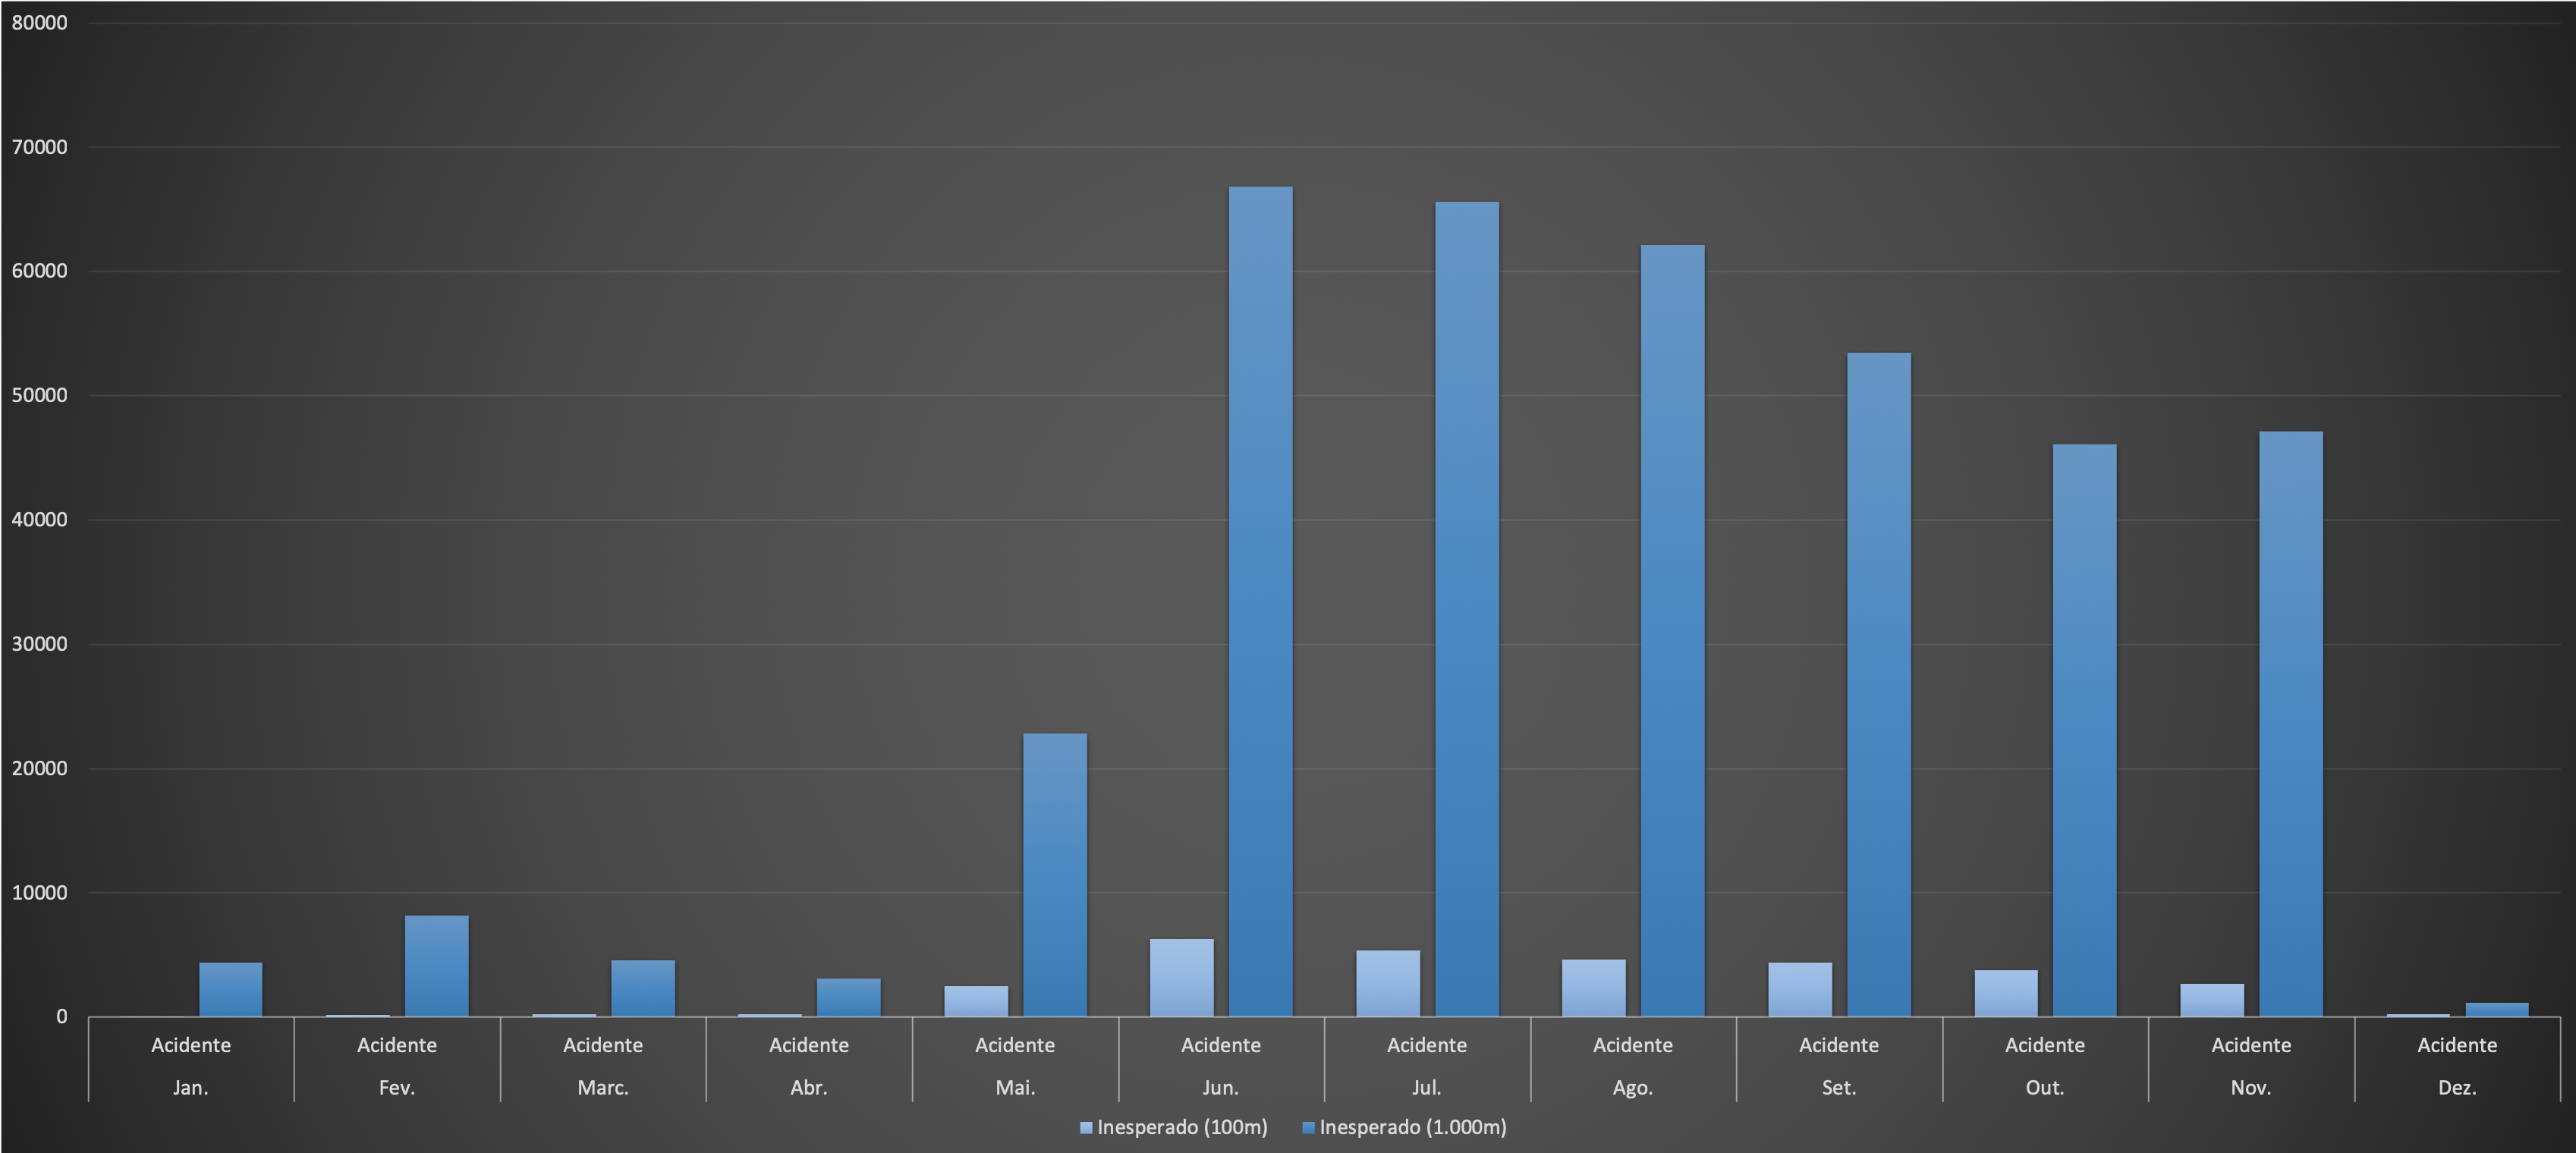
\includegraphics[width=1\linewidth]{images/apriori_analysis_stops_accidents.png}
	\label{fig:apriori_analysis_stops_accidents}
	\source{Felipe Cordeiro Alves Dias (2019)}
\end{figure}

\begin{figure}[!htb]
	\centering
 	  \caption{Velocidades inesperadas dos ônibus impactados por eventos de exceção relacionados a desastres naturais a 100~m e 1.000~m dos pontos de parada, ao longo dos meses do ano de 2017}
		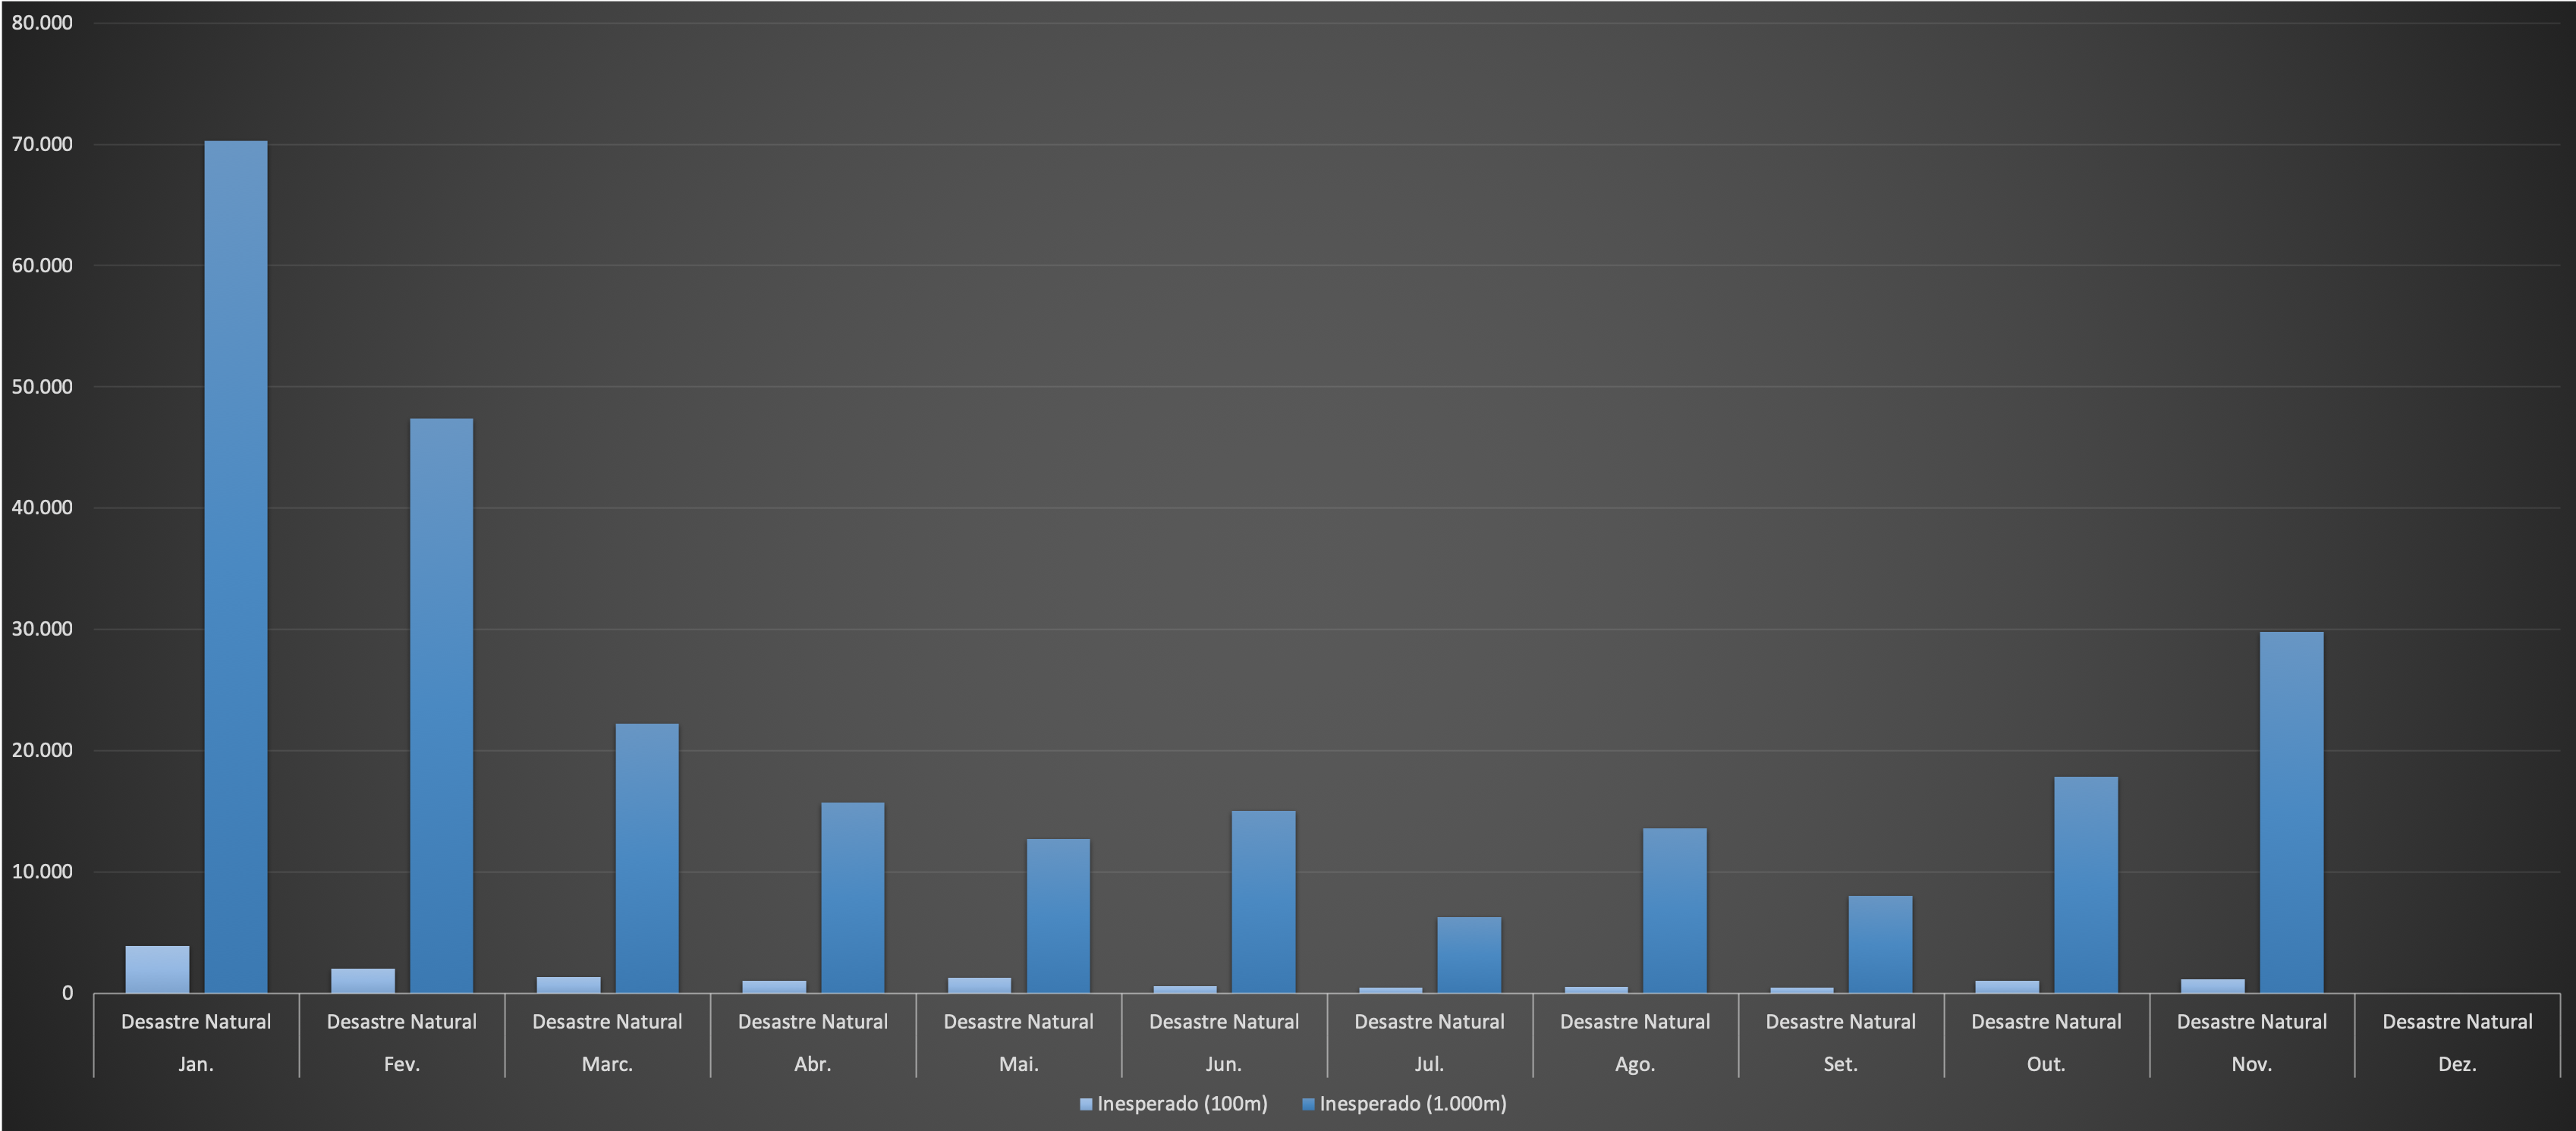
\includegraphics[width=1\linewidth]{images/apriori_analysis_stops_natural_disasters.png}
	\label{fig:apriori_analysis_stops_natural_disasters}
	\source{Felipe Cordeiro Alves Dias (2019)}
\end{figure}

\begin{figure}[!htb]
	\centering
 	  \caption{Velocidades inesperadas dos ônibus impactados por eventos de exceção relacionados a eventos sociais a 100~m e 1.000~m dos pontos de parada, ao longo dos meses do ano de 2017}
		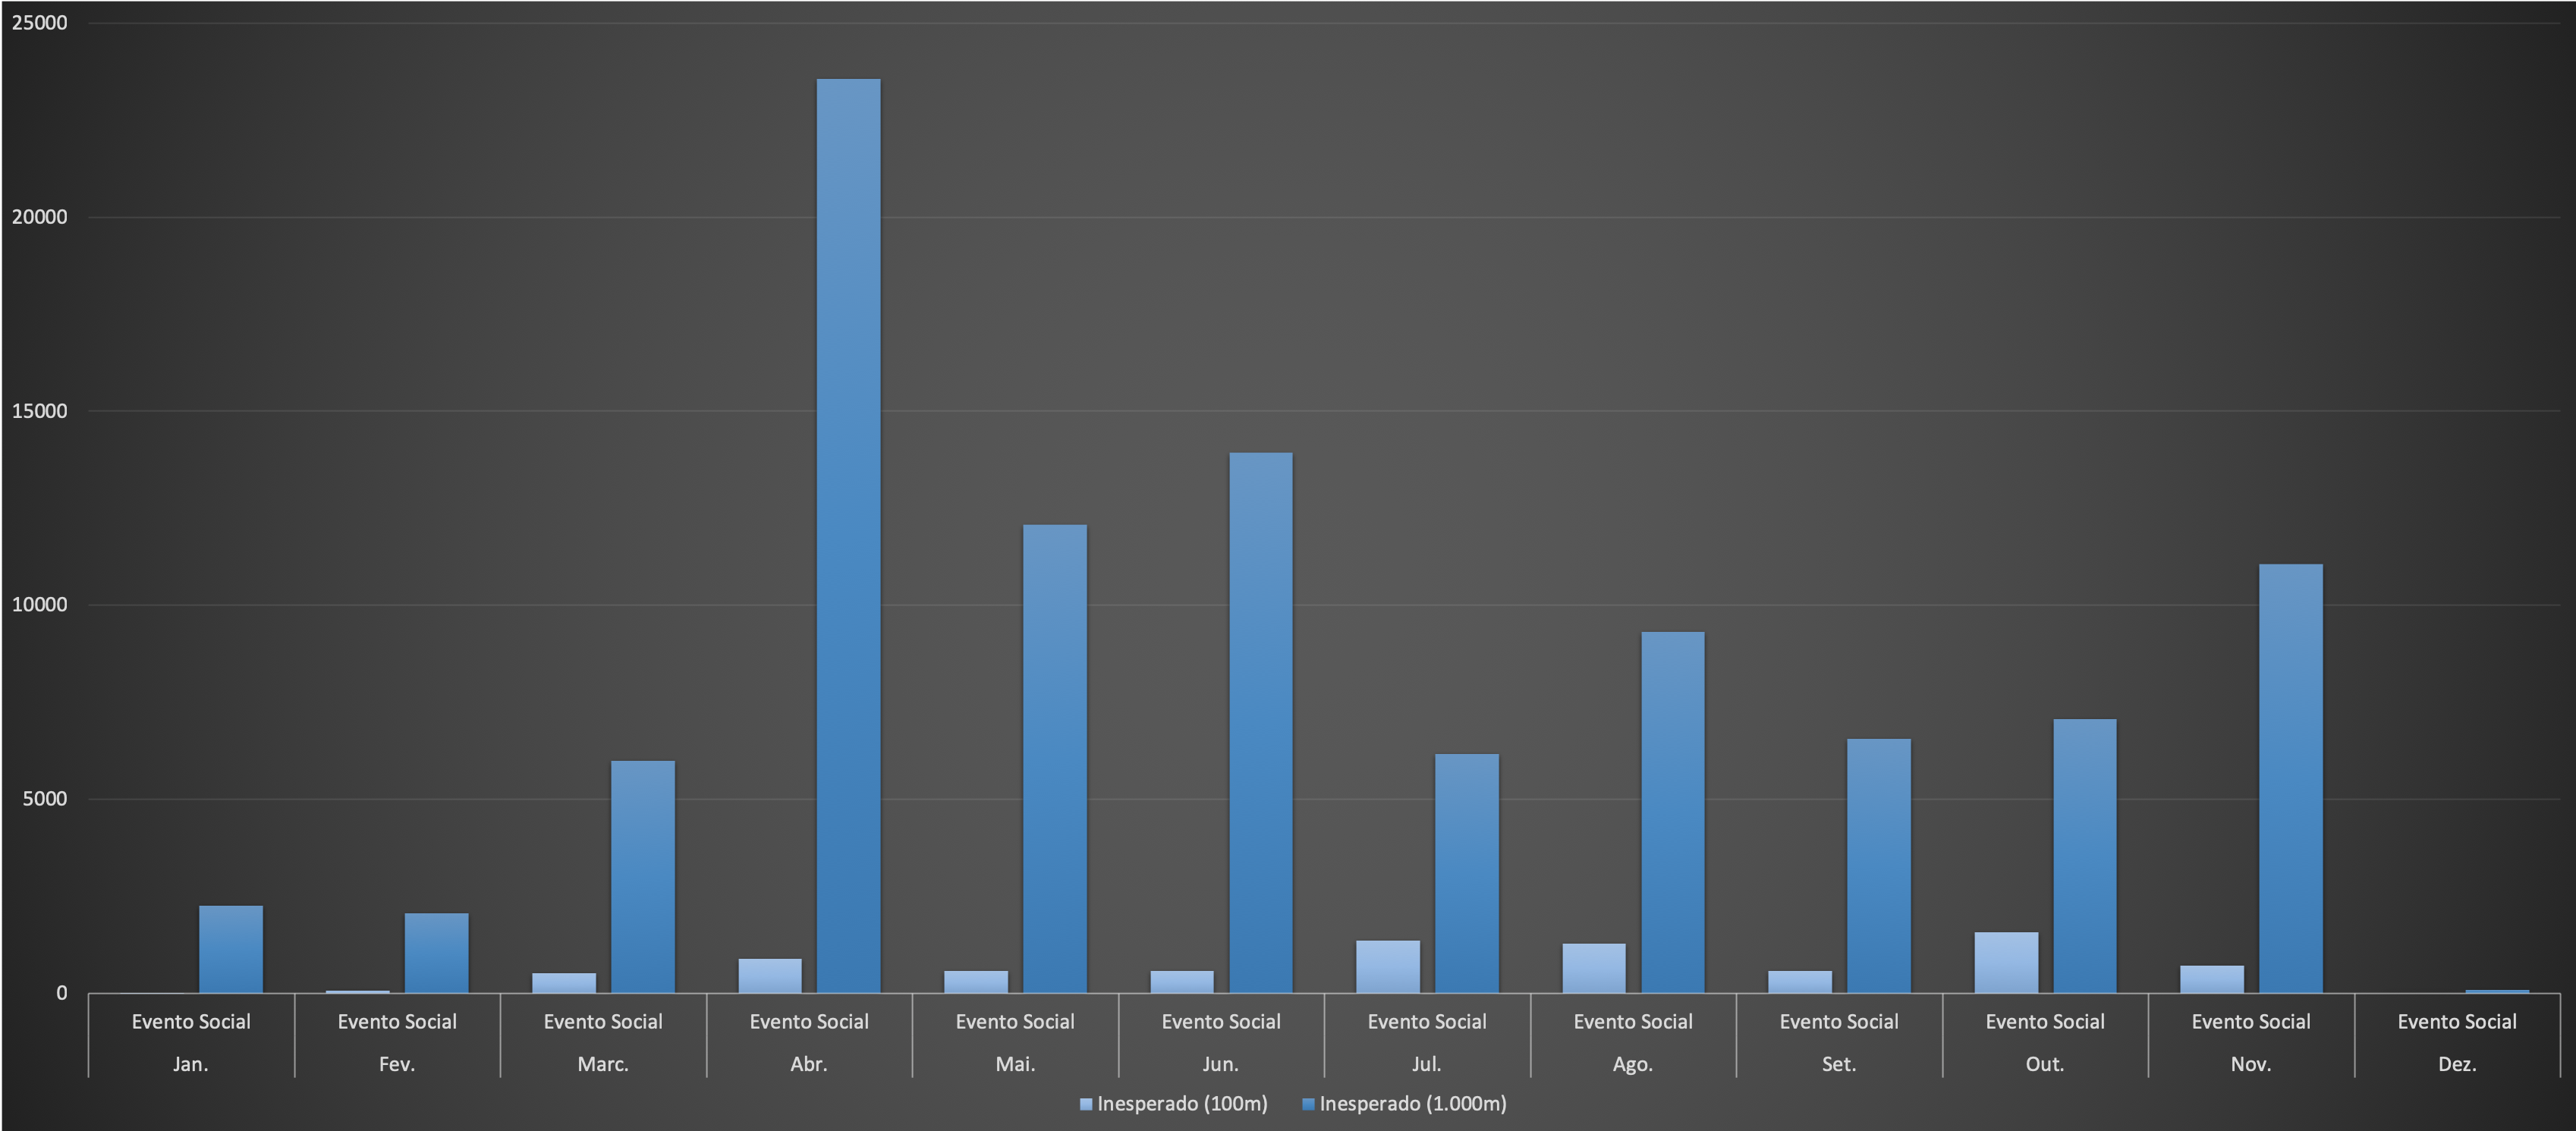
\includegraphics[width=1\linewidth]{images/apriori_analysis_stops_social_events.png}
	\label{fig:apriori_analysis_stops_social_events}
	\source{Felipe Cordeiro Alves Dias (2019)}
\end{figure}

\begin{figure}[!htb]
	\centering
 	  \caption{Velocidades inesperadas dos ônibus impactados por eventos de exceção relacionados a eventos urbanos a 100~m e 1.000~m dos pontos de parada, ao longo dos meses do ano de 2017}
		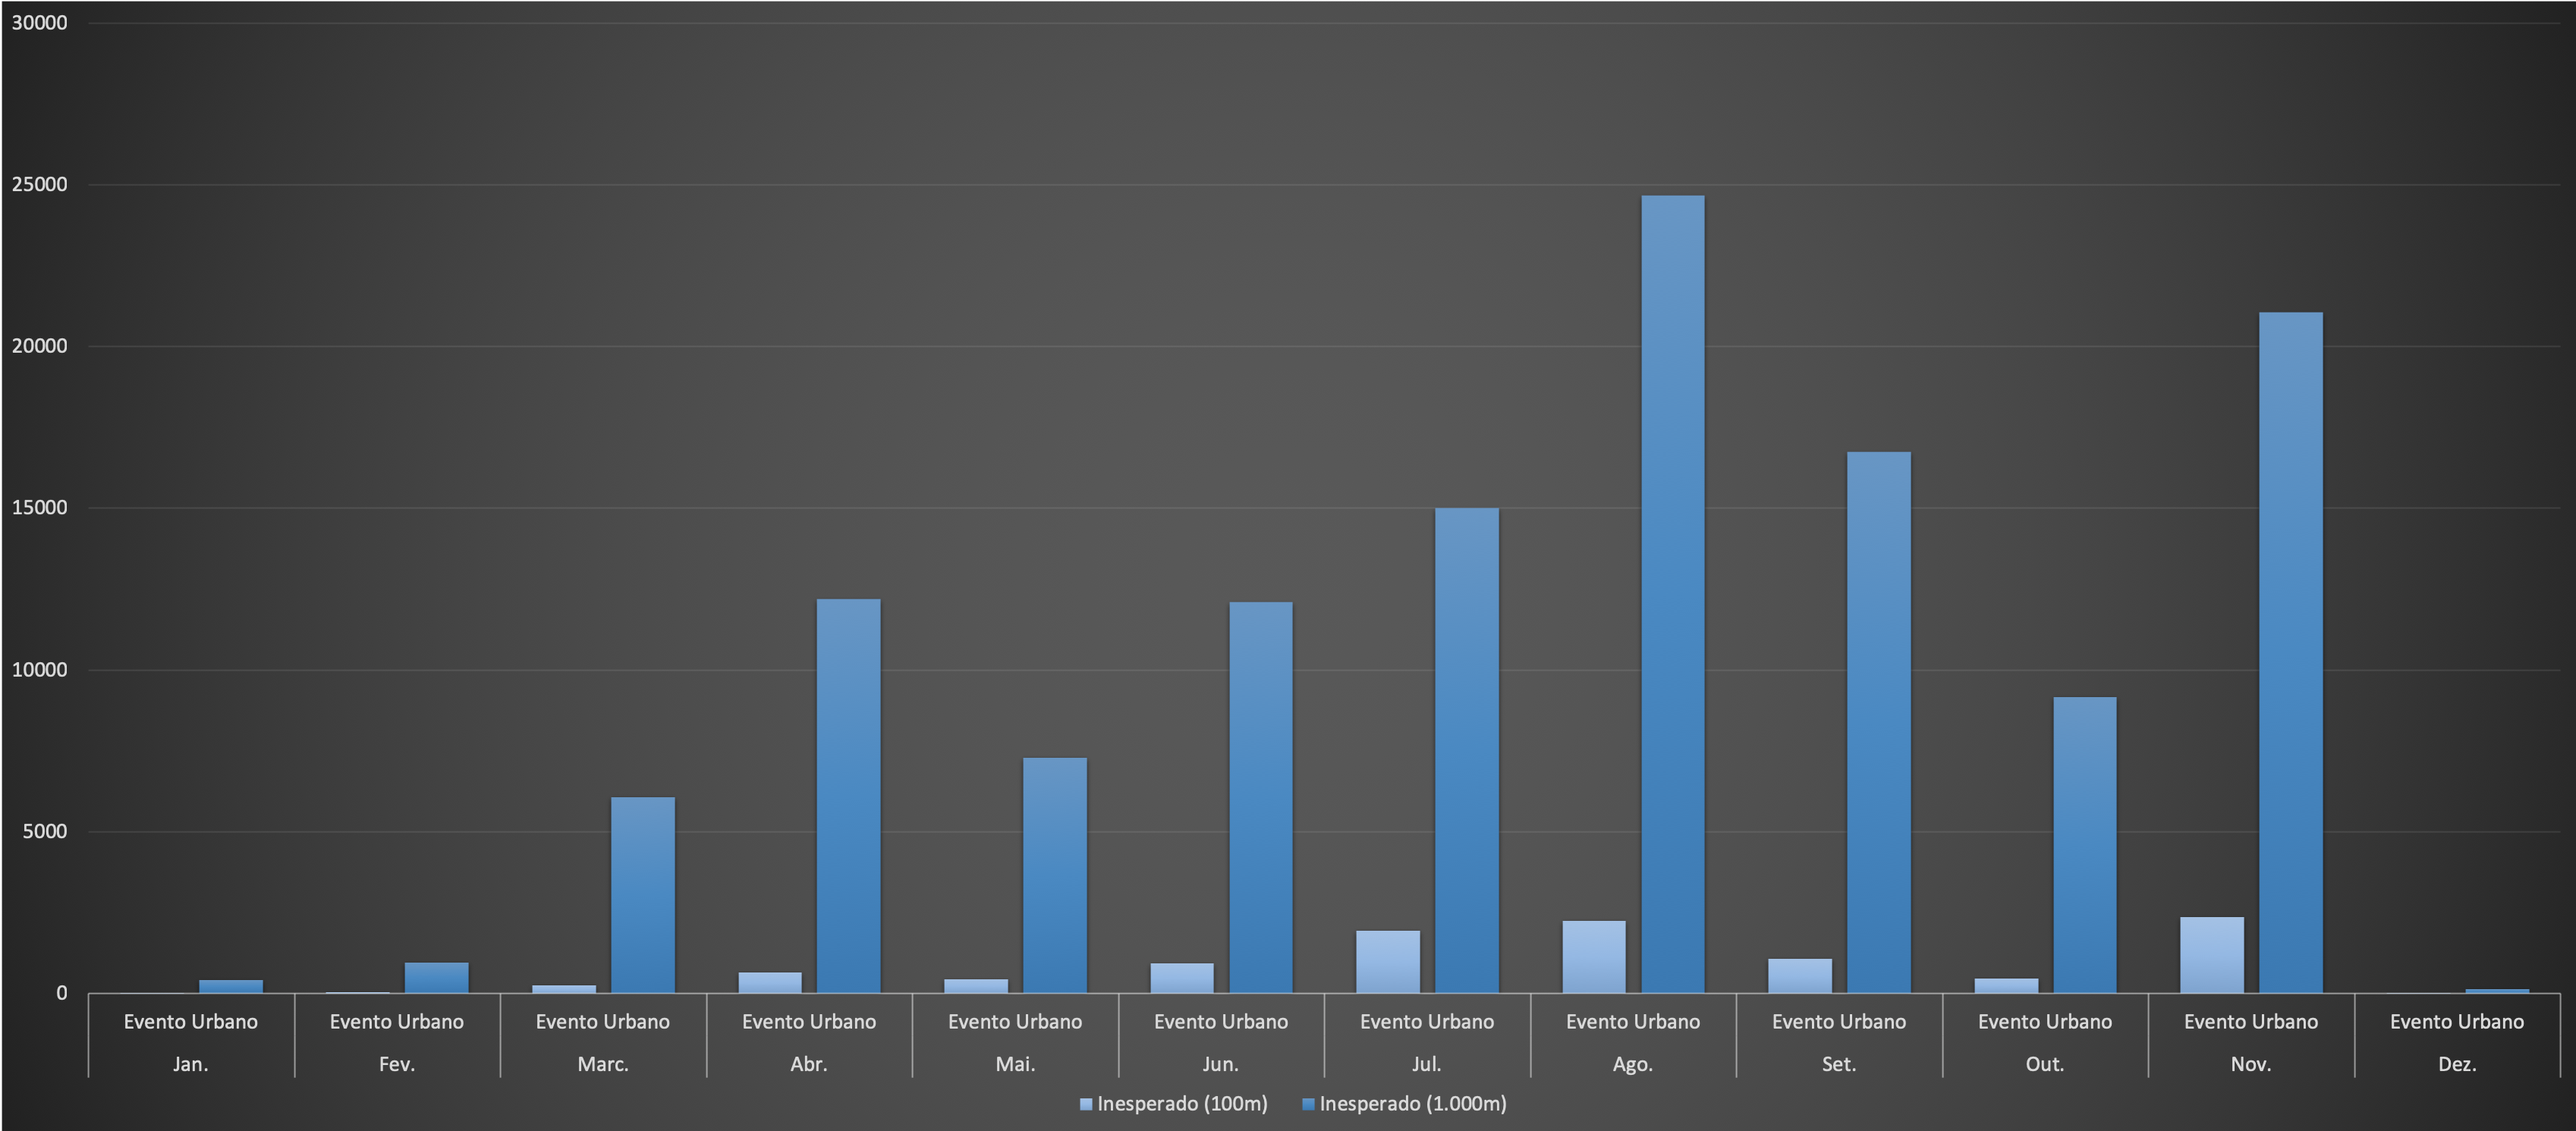
\includegraphics[width=1\linewidth]{images/apriori_analysis_stops_urban_events.png}
	\label{fig:apriori_analysis_stops_urban_events}
	\source{Felipe Cordeiro Alves Dias (2019)}
\end{figure}

\begin{figure}[!htb]
	\centering
 	  \caption{Velocidades inesperadas dos ônibus impactados por eventos de exceção relacionados a acidentes a 100~m e 1.000~m dos pontos de rota, ao longo dos meses do ano de 2017}
		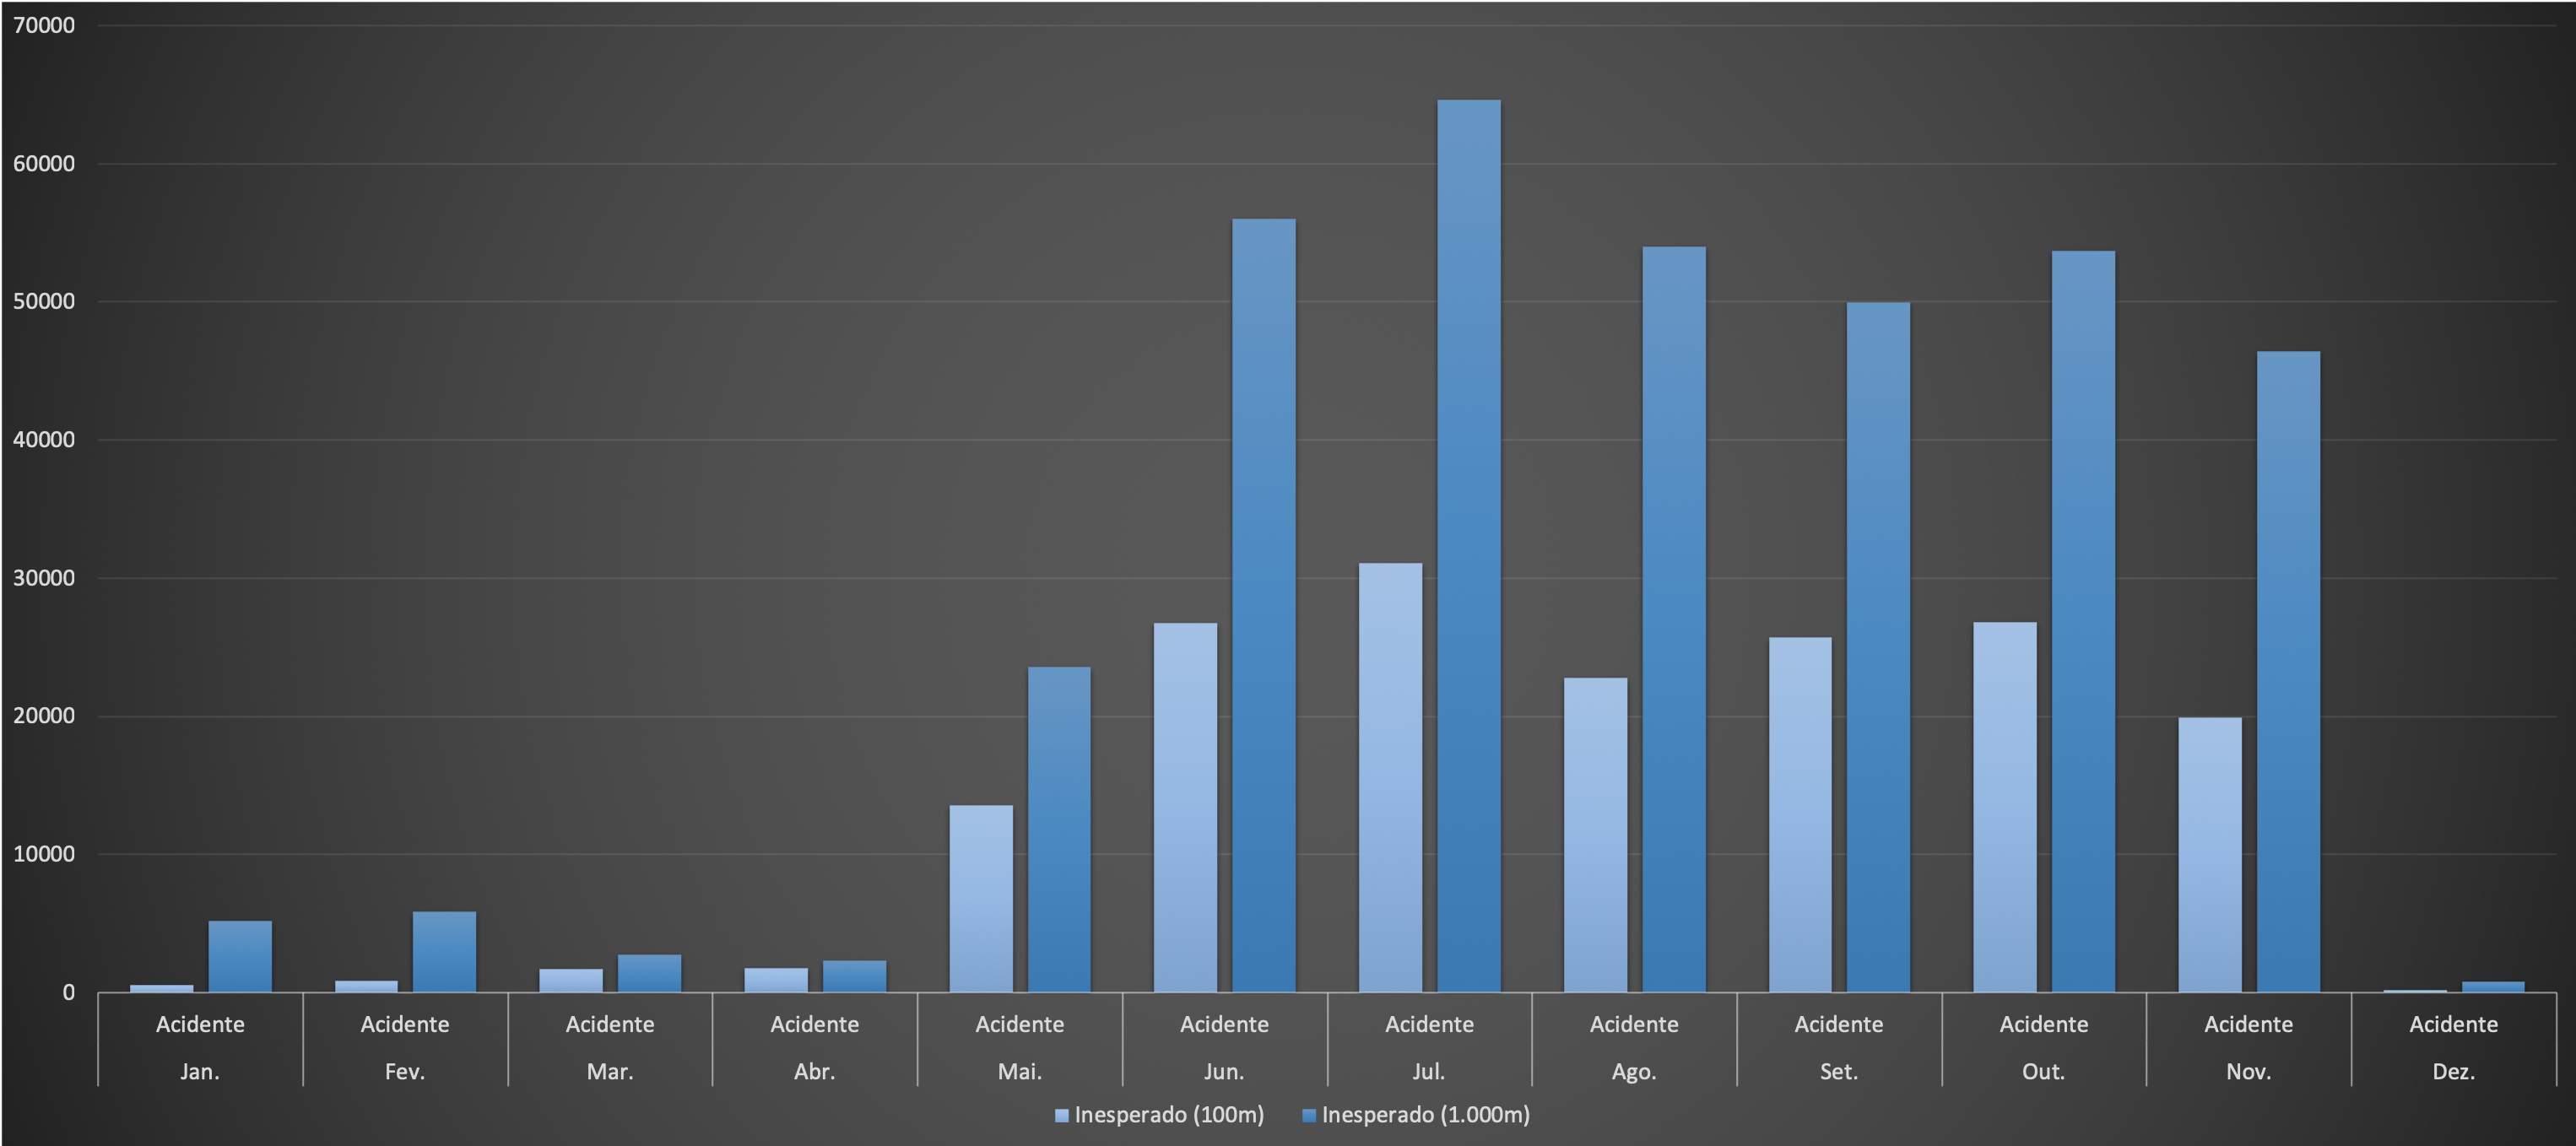
\includegraphics[width=1\linewidth]{images/apriori_analysis_shapes_accidents.png}
	\label{fig:apriori_analysis_shapes_accidents}
	\source{Felipe Cordeiro Alves Dias (2019)}
\end{figure}

\begin{figure}[!htb]
	\centering
 	  \caption{Velocidades inesperadas dos ônibus impactados por eventos de exceção relacionados a desastres naturais a 100~m e 1.000~m dos pontos de rota, ao longo dos meses do ano de 2017}
		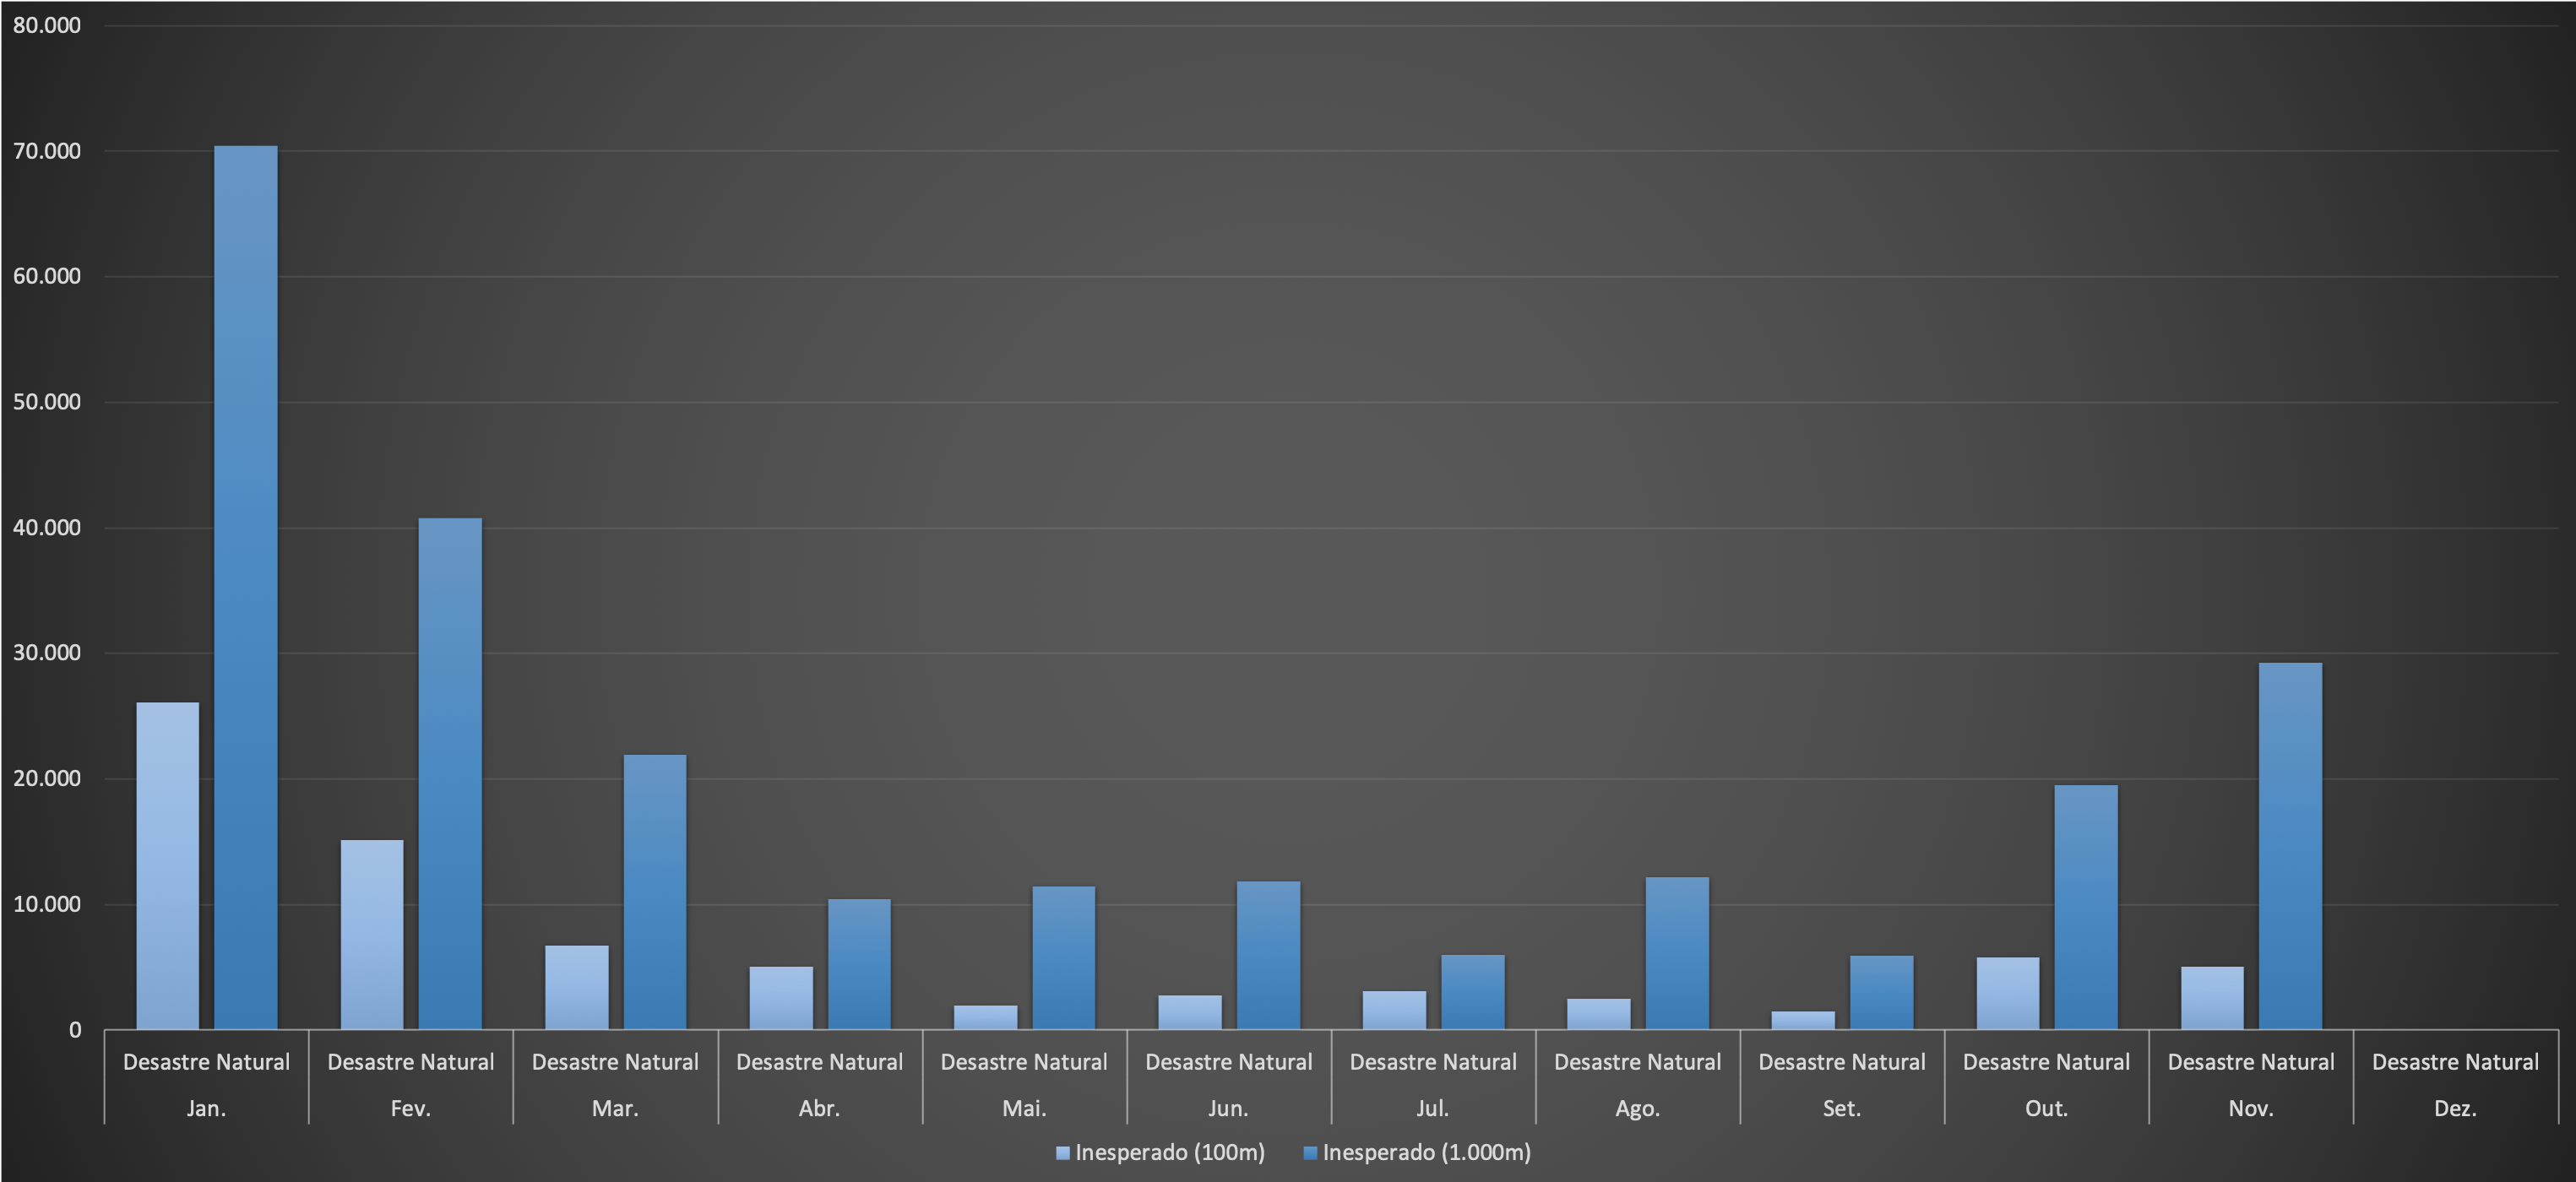
\includegraphics[width=1\linewidth]{images/apriori_analysis_shapes_natural_disasters.png}
	\label{fig:apriori_analysis_shapes_natural_disasters}
	\source{Felipe Cordeiro Alves Dias (2019)}
\end{figure}

\begin{figure}[!htb]
	\centering
 	  \caption{Velocidades inesperadas dos ônibus impactados por eventos de exceção relacionados a eventos sociais a 100~m e 1.000~m dos pontos de rota, ao longo dos meses do ano de 2017}
		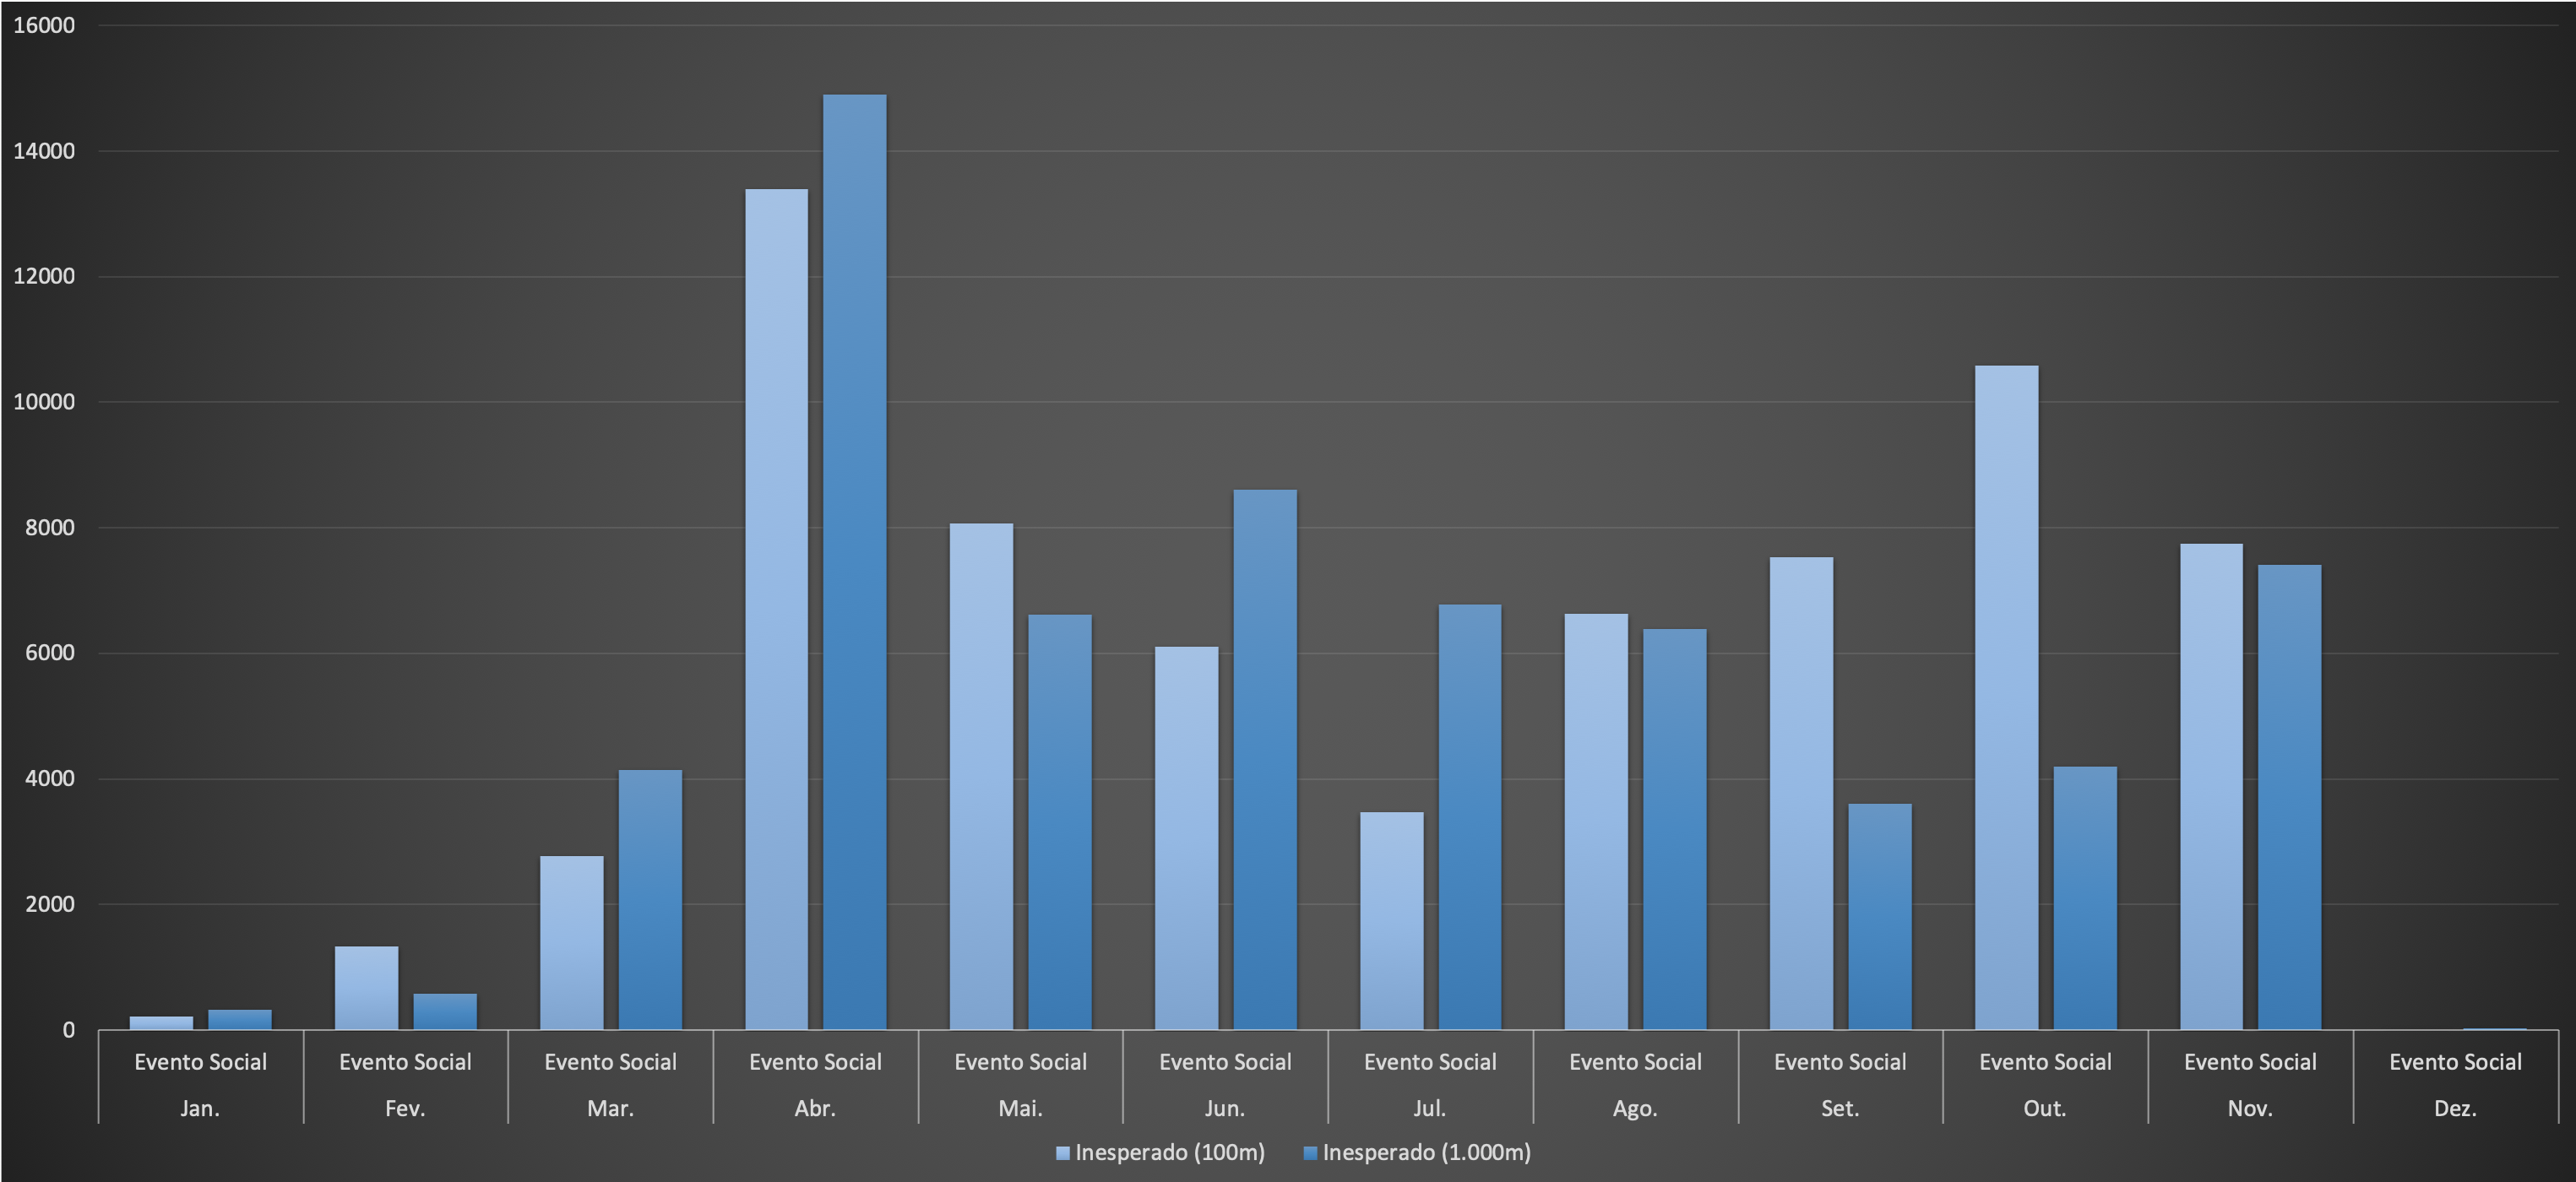
\includegraphics[width=1\linewidth]{images/apriori_analysis_shapes_social_events.png}
	\label{fig:apriori_analysis_shapes_social_events}
	\source{Felipe Cordeiro Alves Dias (2019)}
\end{figure}

\begin{figure}[!htb]
	\centering
 	  \caption{Velocidades inesperadas dos ônibus impactados por eventos de exceção relacionados a eventos sociais a 100~m e 1.000~m dos pontos de rota, ao longo dos meses do ano de 2017}
		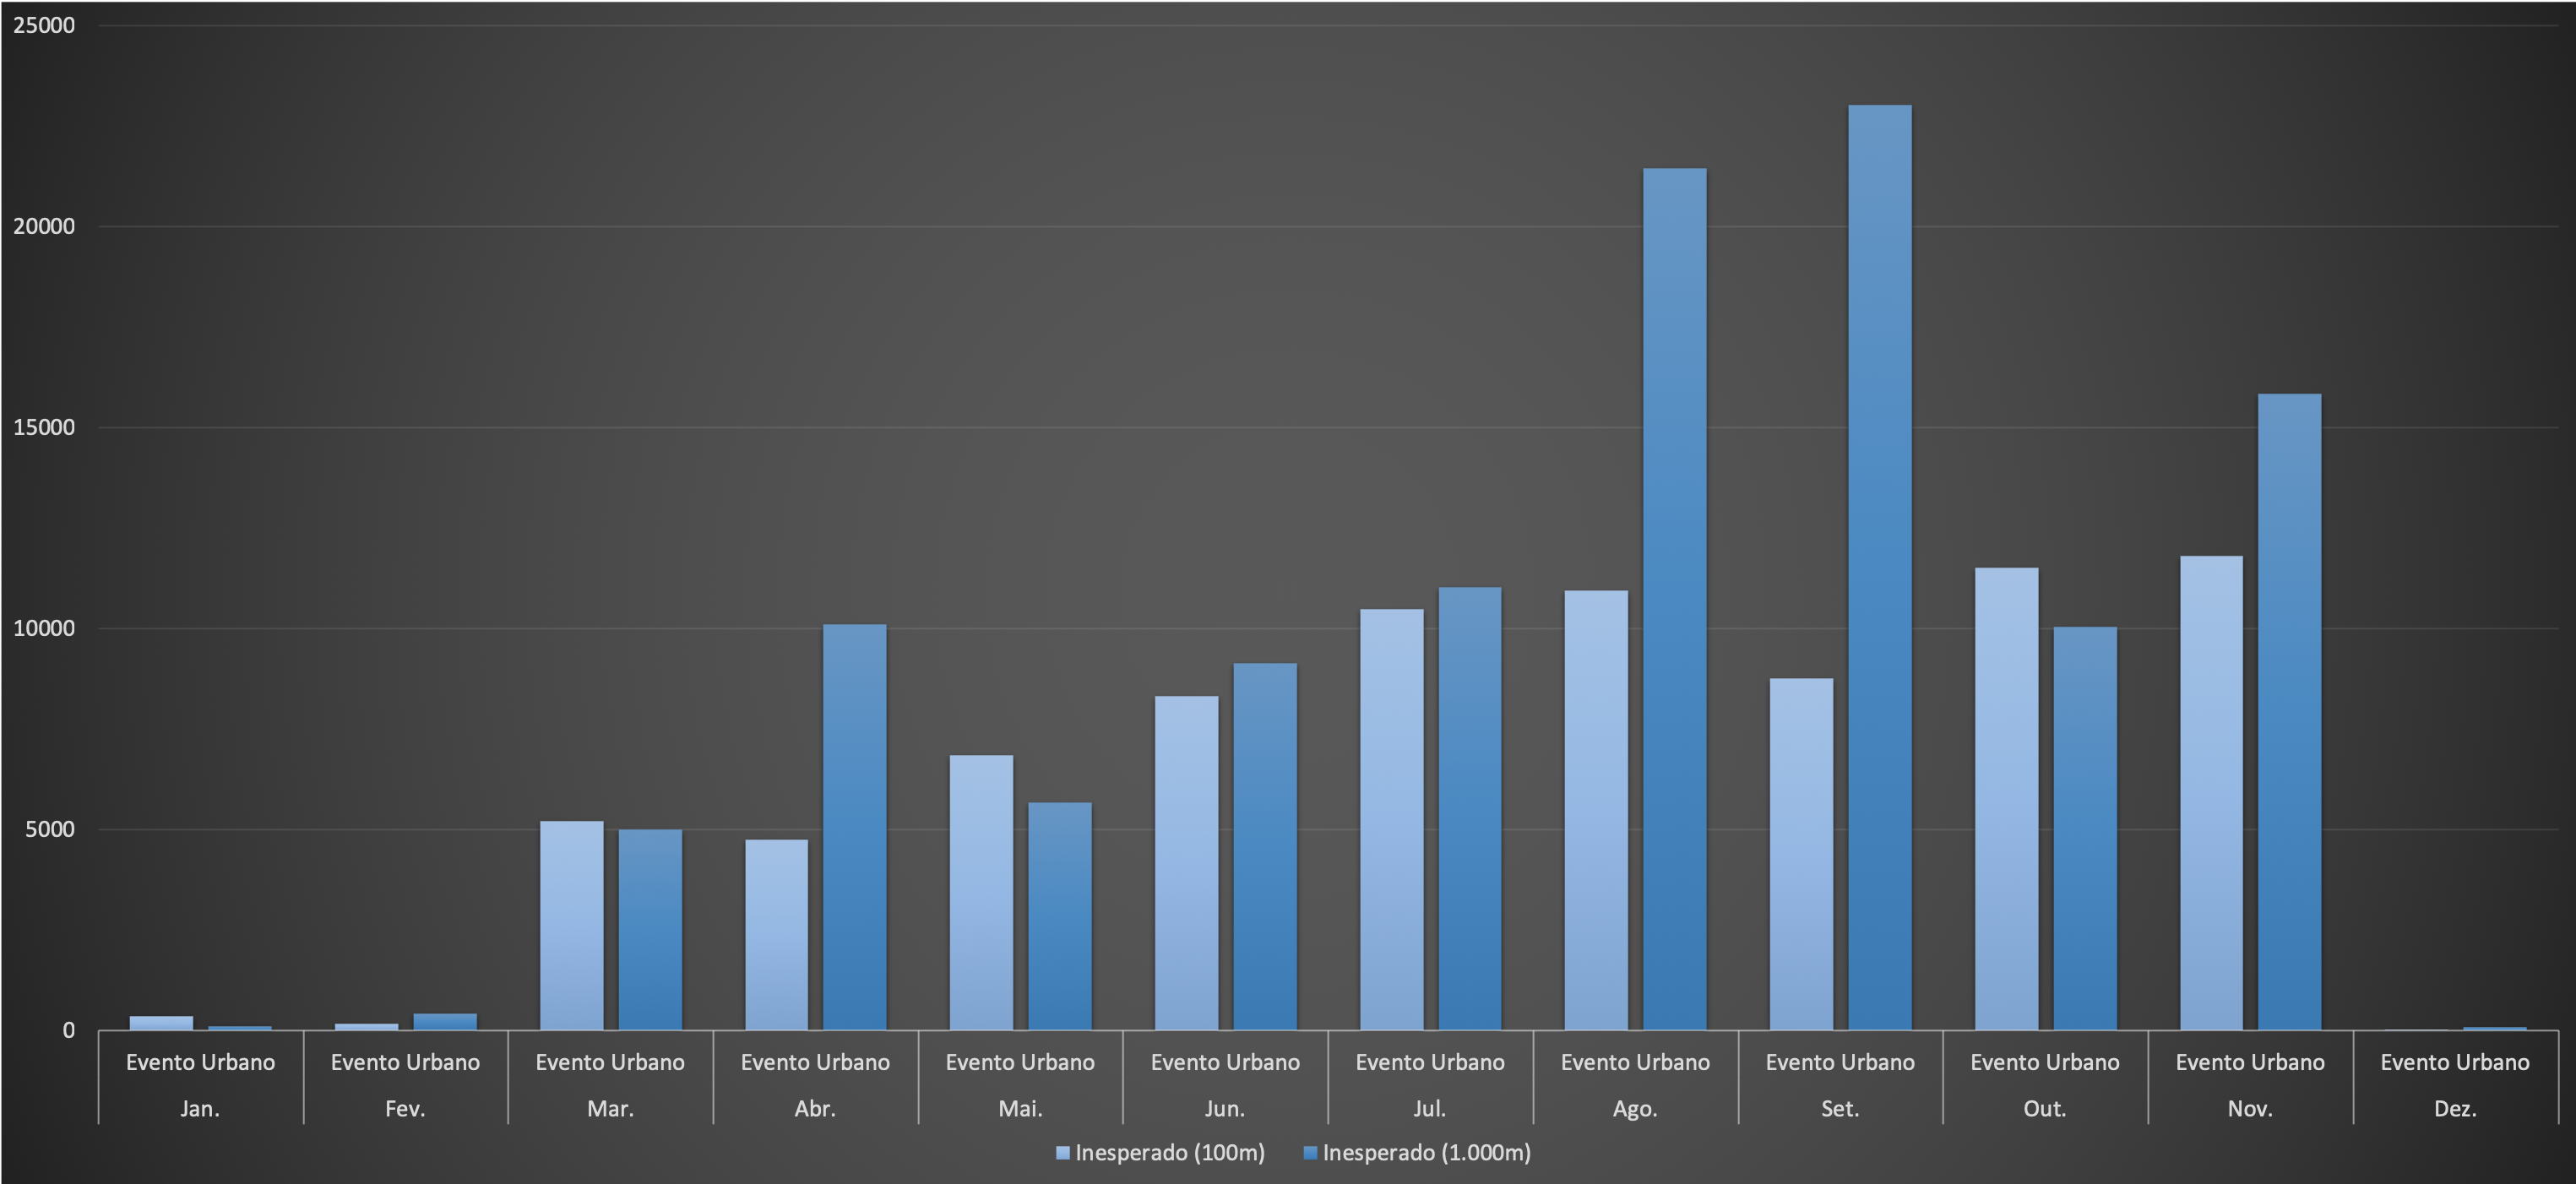
\includegraphics[width=1\linewidth]{images/apriori_analysis_shapes_urban_events.png}
	\label{fig:apriori_analysis_shapes_urban_events}
	\source{Felipe Cordeiro Alves Dias (2019)}
\end{figure}



\begin{table}[!htb]
\centering
\begin{threeparttable}
\caption {Análise \textit{Apriori} aplicada as velocidades médias (intervalos de 5 minutos) ao conjunto de dados AVL da SPTrans correlacionados aos eventos de exceção (a distância de 100~m\tnote{f} e 1.000~m\tnote{g}, respectivamente, dos pontos de parada de ônibus) dos meses do ano de 2017}
\label {tab:aprioriExceptFullStops}
\begin{tabular}{c|c|c|c|c|c}
\toprule
\begin{tabular}{@{}c@{}}\textbf{Classe}\\ \textbf{do evento}\end{tabular} & \begin{tabular}{@{}c@{}}\textbf{Total de}\\ \textbf{eventos}\tnote{a}\end{tabular}  & \begin{tabular}{@{}c@{}}\textbf{Total de Regras }\\ \textbf{de Associação}\tnote{b}\end{tabular}  & \textbf{Esperadas}\tnote{c} & \begin{tabular}{@{}c@{}}\textbf{Não}\\ \textbf{esperadas}\tnote{d}\end{tabular}  & \begin{tabular}{@{}c@{}}\textbf{Parcialmente}\\ \textbf{inesperadas}\tnote{e}\end{tabular} \\
\midrule
Acidente & 1.677 & 315.063 & 278.493 & 30.804 & 5.766 \\
\hline
\begin{tabular}{@{}c@{}}Desastre\\ Natural\end{tabular} &  912 & 115.301 & 99.206 & 14.282 & 1.813 \\
\hline
\begin{tabular}{@{}c@{}}Evento\\ Social\end{tabular} & 506 & 61.927 & 52.403 & 8.245 & 1.279 \\
\hline
\begin{tabular}{@{}c@{}}Evento\\ Urbano\end{tabular}  & 596 & 93.513 & 81.261 & 10.480 & 1.772 \\
\midrule
\textbf{Total} & 3.691 & 585.804 & 511.363 & 63.811 & 10.603 \\
\bottomrule
\toprule
\begin{tabular}{@{}c@{}}\textbf{Classe}\\ \textbf{do evento}\end{tabular} & \begin{tabular}{@{}c@{}}\textbf{Total de}\\ \textbf{eventos}\tnote{a}\end{tabular}  & \begin{tabular}{@{}c@{}}\textbf{Total de Regras }\\ \textbf{de Associação}\tnote{b}\end{tabular}  & \textbf{Esperadas}\tnote{c} & \begin{tabular}{@{}c@{}}\textbf{Não}\\ \textbf{esperadas}\tnote{d}\end{tabular}  & \begin{tabular}{@{}c@{}}\textbf{Parcialmente}\\ \textbf{inesperadas}\tnote{e}\end{tabular} \\
\midrule
Acidente & 3.029 & 3.980.542 & 3.415.780 & 385.728 & 179.034 \\
\hline
\begin{tabular}{@{}c@{}}Desastre\\ Natural\end{tabular} &  2.016 & 2.624.415 & 2.253.123 & 259.285 & 112.007 \\
\hline
\begin{tabular}{@{}c@{}}Evento\\ Social\end{tabular} & 764 & 1.262.805 & 1.118.546 & 100.224 & 44.035 \\
\hline
\begin{tabular}{@{}c@{}}Evento\\ Urbano\end{tabular}  & 980 & 1.481.040 & 1.296.476 & 125.803 & 58.761 \\
\midrule
\textbf{Total} & 6.789 & 9.348.802 & 8.083.925 & 871.040 & 393.837 \\
\bottomrule
\end{tabular}
\begin{tablenotes}
            \item[a] Total de eventos de exceção.
            \item[b] Total de correlações de velocidade média.
            \item[c] Regras esperadas ($Lift > 1$, $Support > 0,05$)
            \item[d] Regras de associação inesperadas ($Lift = 1$).
            \item[e] Regras de associação parcialmente inesperadas ($0 < Lift < 1$).
            \item[f] 3.545 eventos de exceção não atingiram linhas de ônibus no raio de 100~m.
            \item[g] 447 eventos de exceção não atingiram linhas de ônibus no raio de 1.000~m.
        \end{tablenotes}
\end{threeparttable}
\source{Felipe Cordeiro Alves Dias (2019)}
\end{table}

\begin{table}[!htb]
\centering
\begin{threeparttable}
\caption {Análise \textit{Apriori} aplicada as velocidades médias (intervalos de 5 minutos) ao conjunto de dados AVL da SPTrans correlacionados aos eventos de exceção (a distância de 100~m\tnote{g} e 1.000~m\tnote{h}, respectivamente, dos pontos de rota dos ônibus) dos meses do ano de 2017}
\label {tab:aprioriExceptFullShapes}
\begin{tabular}{c|c|c|c|c|c}
\toprule

%\begin{tabular}{@{}c@{}}Desastre\\ Natural\end{tabular} 
%\begin{tabular}{@{}c@{}}Evento\\ Social\end{tabular} 
%\begin{tabular}{@{}c@{}}Evento\\ Urbano\end{tabular} 

\begin{tabular}{@{}c@{}}\textbf{Classe}\\ \textbf{do Evento}\end{tabular} & \begin{tabular}{@{}c@{}}\textbf{Total de}\\ \textbf{Eventos}\tnote{b}\end{tabular}   & \begin{tabular}{@{}c@{}}\textbf{Qtd. Regras }\\ \textbf{de Associação}\tnote{c}\end{tabular}  & \textbf{Esperadas}\tnote{d} & \begin{tabular}{@{}c@{}}\textbf{Não}\\ \textbf{Esperadas}\tnote{e}\end{tabular} & \begin{tabular}{@{}c@{}}\textbf{Parcialmente}\\ \textbf{inesperadas}\tnote{f}\end{tabular}    \\
\midrule
Acidente & 2.367 & 3.390.690 & 3.164.726 & 171.860 & 54.104 \\
\hline
\begin{tabular}{@{}c@{}}Desastre\\ Natural\end{tabular} & 1.307 & 1.342.048 & 1.247.219 & 75.981 & 18.848 \\
\hline
\begin{tabular}{@{}c@{}}Evento\\ Social\end{tabular} & 704 & 1.522.423 & 1.433.700 & 67.835 & 20.888 \\
\hline
\begin{tabular}{@{}c@{}}Evento\\ Urbano\end{tabular}  & 825 & 1.602.343 & 1.499.305 & 79.155 & 23.883 \\
\midrule
\midrule \textbf{Total} & 5.203 & 7.857.504 & 7.344.950 & 394.831 & 117.723 \\
\bottomrule
\toprule
\begin{tabular}{@{}c@{}}\textbf{Classe}\\ \textbf{do evento}\end{tabular} & \begin{tabular}{@{}c@{}}\textbf{Total de}\\ \textbf{eventos}\tnote{a}\end{tabular}  & \begin{tabular}{@{}c@{}}\textbf{Total de Regras }\\ \textbf{de Associação}\tnote{b}\end{tabular}  & \textbf{Esperadas}\tnote{c} & \begin{tabular}{@{}c@{}}\textbf{Não}\\ \textbf{esperadas}\tnote{d}\end{tabular}  & \begin{tabular}{@{}c@{}}\textbf{Parcialmente}\\ \textbf{inesperadas}\tnote{e}\end{tabular} \\
\midrule
Acidente & 3.035 & 2.772.368 & 2.259.806 & 365.234 & 147.328 \\
\hline
\begin{tabular}{@{}c@{}}Desastre\\ Natural\end{tabular} & 2017 & 1.876.843 & 1.545.172 & 239.897 & 91.774 \\
\hline
\begin{tabular}{@{}c@{}}Evento\\ Social\end{tabular}  & 764 & 683.037 & 588.385 & 63.549 & 31.103 \\
\hline
\begin{tabular}{@{}c@{}} Evento\\ Urbano\end{tabular}  & 980 & 963.892 & 805.901 & 111.898 & 46.093 \\
\midrule
\midrule \textbf{Total} & 6.796 & 6.296.140 & 5.199.264 & 780.578 & 316.298 \\
\bottomrule
\end{tabular}
\begin{tablenotes}
            \item[a] Total de eventos de exceção.
            \item[b] Total de correlações de velocidade média.
            \item[c] Regras esperadas ($Lift > 1$, $Support > 0,05$)
            \item[d] Regras de associação inesperadas ($Lift = 1$).
            \item[e] Regras de associação parcialmente inesperadas ($0 < Lift < 1$).
            \item[f] 2.033 eventos de exceção não atingiram linhas de ônibus no raio de 100~m.
            \item[g] 440 eventos de exceção não atingiram linhas de ônibus no raio de 1.000~m.
        \end{tablenotes}
\end{threeparttable}
\source{Felipe Cordeiro Alves Dias (2019)}
\end{table}

\clearpage

\section{Considerações sobre a caracterização dos impactos dos eventos de exceção}

De acordo com experimentos realizados, conseguimos caracterizar padrões inesperados e reduções de velocidades relacionadas aos eventos de exceção. Tais padrões foram validados de acordo com os períodos de sazonalidade e dos eventos de exceção identificados nos \textit{tweets}. Além disso, encontramos notícias veiculadas na mídia correlacionadas aos padrões identificados, o que também valida as caracterizações realizadas.

\chapter{Conclusão}
\label{conclusion}

Neste capítulo, são apresentadas as contribuições e resultados esperados com o projeto de pesquisa, as limitações a ameaças à validade do estudo. 

\section{Contribuições}

A principal contribuição deste projeto é o estudo realizado para caracterização de eventos de exceção e de seus respectivos impactos no sistema de transporte público por ônibus da cidade de São Paulo, por meio de \textit{tweets}, dados históricos dos módulos AVL do SIM e da GTFS. %Além disso, a solução proposta visa disponibilizar os conjuntos de dados que foram construídos e uma plataforma para que esses dados possam ser visualizados e explorados, de forma a contribuir com projetos e pesquisas futuras correlatas. 
Também, validamos uma metodologia para extração e geolocalização dos endereços contidos nas publicações dos órgãos responsáveis por reportar eventos de exceção da cidade de São Paulo. Além disso, propomos uma arquitetura distribuída para exploração e visualização de dados AVL.

Por fim, a abordagem que utiliza as coordenadas espaciais dos pontos de parada de ônibus como referência pode ser mais adequada do que a que usa os pontos de rota. Isso, devido aos resultados semelhantes obtidos, menor custo computacional e margem de erro. 

\section{Trabalhos publicados}

DIAS, F. C. A.; Cordeiro, D. \textit{Visualizing large datasets: A case study with data of the buses of São Paulo city}. \textit{In}: \textit{1st Workshop on the Distributed Smart City} (WDSC'2018), 2018, Salvador, BA. \textit{Proceedings of the 37th IEEE International Symposium on Reliable Distributed Systems}, 2018. p. 10-13.

\section{Trabalhos submetidos}

DIAS, F.C.A; Cordeiro, D. \textit{Characterization of exception events and their respective impacts on the public transport system by bus of São Paulo}. Simpósio Brasileiro de Redes de Computadores e Sistemas Distribuídos (SBRC), 2019.

\section{Trabalhos futuros}
Como trabalho futuro, pretendemos implementar o fluxo de processamento de dados em \textit{streaming} mencionado na Figura~\ref{fig:viz_arch}, em um cenário de exploração e visualização de dados quase em tempo real.  Além disso, há a necessidade de estabelecermos uma cooperação entre a Acadêmia e a SPTrans para aplicação cotidiana dos experimentos realizados por esse trabalho e outros relacionados a análise de grandes volumes de dados de transportes públicos. Outra possibilidade futura é a de aplicar os experimentos realizados por este trabalho a publicações de usuários que representam a sociedade civil.

% ----------------------------------------------------------
% ELEMENTOS PÓS-TEXTUAIS
% ----------------------------------------------------------
\postextual
% ----------------------------------------------------------

% ----------------------------------------------------------
% Referências bibliográficas
% ----------------------------------------------------------
%\listoftodos[Notes]
\bibliography{referencias}

% ----------------------------------------------------------
% Glossário
% ----------------------------------------------------------
%
% Consulte o manual da classe abntex2 para orientações sobre o glossário.
%
%\glossary

% ----------------------------------------------------------
% Apêndices
% ----------------------------------------------------------

% ---
% Inicia os apêndices
% ---
\begin{apendicesenv}

% Imprime uma página indicando o início dos apêndices
%\partapendices
\chapter{Exemplos de \textit{tweets}}
\label{apendiceA}

Neste apêndice, listamos como exemplos alguns \textit{tweets} das contas selecionadas.

\begin{lstlisting}[language=json,title=Exemplos de \textit{tweets} dos perfis selecionados citados na Tabela~\ref{tab:oficialProfiles}, label=tweetsSample]
{
    "tweet_id" : 895060642952077314,
    "tweet_account": "BombeirosPMESP",
    "text" : "19h58 Colisão de Carro x Caminhão, Estrada Sta Isabel, 5950 Itaquaquecetuba. 2 Vítimas, 1 Vtr. Aguardando maiores informes"
}
{
    "tweet_id" : 894707930217447427,
    "tweet_account": "CETSP_",
    "text" : "Referente manifestação Rua Augusta, pista liberada.#ZC"
}
{
    "tweet_id" : 894147793060716544,
    "tweet_account": "CPTM_oficial",
    "text" : "#L11 Hoje, das 8h à meia-noite, circulação interrompida entre Luz e Brás. P/ seguir viagem, use a L7-Rubi q prestará serviço até a Est. Brás"
}
{
    "tweet_id" : 895054721026838530,
    "tweet_account": "governosp",
    "text" : "@SANROGE Lamentamos o ocorrido, Rogerio. Estamos trabalhando continuamente para melhorar a segurança na região. Entre maio e junho, [+] [1]"
}
{
    "tweet_id" : 895000711284621312,
    "tweet_account": "metrosp_oficial",
    "text" : "08/08/2017 16:16: #metrosp : Linha 5-Lilás: Velocidade Reduzida. Mais informações em https://t.co/CaeqD26iJR"
}
{
    "tweet_id" : 884039273493803008,
    "tweet_account": "PMESP",
    "text" : "AGORA: Desfile Cívico-Militar de 9 de Julho no Obelisco - Ibirapuera SP, transmissão ao vivo na página oficial Facebook da Polícia Militar.",
    "dateTime" : "2017-07-09 10:19:22"
}
{
    "tweet_id" : 887315002117500932,
    "tweet_account": "Policia_Civil",
    "text" : "Polícia Civil realiza operação para combater a prática do Jogo conhecido como "Baleia Azul"... https://t.co/kh2HW6UZvT",
}
{
    "tweet_id" : 895004079910518788,
    "tweet_account": "saopaulo_agora",
    "text" : "#ItaimPaulista Incêndio na Rua Mateus Barbosa de Resende nº 235. Defesa Civil Regional acionada para o local. (CCOI) #spagora"
}
{
    "tweet_id" : 894694704989732864,
    "tweet_account": "smtpsp_",
    "text" : "A @sptrans_ irá modificar 14 linhas na Zona Leste para obras no Monotrilho Saiba mais: https://t.co/fCA0T7WCSY"
}
{
    "tweet_id" : 902953598857949184,
    "tweet_account": "SPCEDEC",
    "text" : "30-08-2017 - Acidente com produto perigoso em  com 36 , deixa 21 vítimas feridas e 02 ."
}
{
    "tweet_id" : 895065137484320769,
    "tweet_account": "sptrans_",
    "text" : "Obras do Monotrilho desviam itinerários de 14 linhas que atendem a Av. Sapopemba entre 5 e 11/08, das 23h às 5h: https://t.co/jH4LFgrSKZ"
}
{
    "tweet_id : 895042604068458497,
    "tweet_account": "TurismoSaoPaulo",
    "text" : "Veganos, vegetarianos e simpatizantes: vem aí o Vegan Club, em 12/08, no Centro de SP! #crueltyfree #veganfood... https://t.co/7f7ggr4vn4"
}
\end{lstlisting}

\clearpage

\chapter{Logradouros utilizados}
\label{apendiceB}

Neste apêndice, listamos os logradouros utilizados como referência no processo de extração dos endereços dos \textit{tweets}.

\begin{longtable}{c|c}
\caption{Tabela de logradouros com abreviaturas}
\label{tab:logradouros}\\

\hline \multicolumn{1}{c |}{\textbf{Abreviatura}} & \multicolumn{1}{c}{\textbf{Logradouro}} \\ \hline 
\endfirsthead

\multicolumn{2}{c}%
{{\bfseries \tablename\ \thetable{} -- continuação da página anterior}} \\
\hline \multicolumn{1}{c |}{\textbf{Abreviatura}} & \multicolumn{1}{c}{\textbf{Logradouro}}  \\ \hline 
\endhead

\hline \multicolumn{2}{r}{{Continua na próxima página}} \\
\endfoot

\hline \hline
\endlastfoot

\hline
ACAMP & Acampamento \\
\hline
AC & Acesso \\
\hline
AD & Adro \\
\hline
ERA & Aeroporto \\
\hline
AL & Alameda \\
\hline
AT & Alto \\
\hline
A & Área \\
\hline
AE & Área especial \\
\hline
ART & Artéria \\
\hline
ATL & Atalho \\
\hline
AV & Avenida \\
\hline
AV-CONT & Avenida contorno \\
\hline
BX & Baixa \\
\hline
BLO & Balão \\
\hline
BAL & Balneário \\
\hline
BC & Beco \\
\hline
BELV & Belvedere \\
\hline
BL & Bloco \\
\hline
BSQ & Bosque \\
\hline
BVD & \textit{Boulevard} \\
\hline
BCO & Buraco \\
\hline
C & Cais \\
\hline
CALC & Calcada \\
\hline
CAM & Caminho \\
\hline
CPO & Campo \\
\hline
CAN & Canal \\
\hline
CHAP & Chácara \\
\hline
CHAP & Chapadão \\
\hline
CIRC & Circular \\
\hline
COL & Colonia \\
\hline
CMP-VR & Complexo viário \\
\hline
COND & Condomínio \\
\hline
CJ & Conjunto \\
\hline
COR & Corredor \\
\hline
CRG & Córrego \\
\hline
DSC & Descida \\
\hline
DSV & Desvio \\
\hline
DT & Distrito \\
\hline
EVD & Elevada \\
\hline
ENT-PART & Entrada particular \\
\hline
EQ & Entre quadra \\
\hline
ESC & Escada \\
\hline
ESP & Esplanada \\
\hline
ETC & Estação \\
\hline
ESTC & Estacionamento \\
\hline
ETD & Estadio \\
\hline
ETN & Estancia \\
\hline
EST & Estrada \\
\hline
EST-MUN & Estrada municipal \\
\hline
FAV & Favela \\
\hline
FAZ & Fazenda \\
\hline
FRA & Feira \\
\hline
FER & Ferrovia \\
\hline
FNT & Fonte \\
\hline
FTE & Forte \\
\hline
GAL & Galeria \\
\hline
GJA & Granja \\
\hline
HAB & Habitacional \\
\hline
IA & Ilha \\
\hline
JD & Jardim \\
\hline
JDE & Jardinete \\
\hline
LD & Ladeira \\
\hline
LG & Lago \\
\hline
LGA & Lagoa \\
\hline
LRG & Largo \\
\hline
LOT & Loteamento \\
\hline
MNA & Marina \\
\hline
MOD & Modulo \\
\hline
TEM & Monte \\
\hline
MRO & Morro \\
\hline
NUC & Núcleo \\
\hline
PDA & Parada \\
\hline
PDO & Paradouro \\
\hline
PAR & Paralela \\
\hline
PRQ & Parque \\
\hline
PSG & Passagem \\
\hline
PSC-SUB & Passagem subterrânea \\
\hline
PSA & Passarela \\
\hline
PAS & Passeio \\
\hline
PAT & Patio \\
\hline
PNT & Ponta \\
\hline
PTE & Ponte \\
\hline
PTO & Porto \\
\hline
PC & Praça \\
\hline
PC-ESP & Praça de esportes \\
\hline
PR & Praia \\
\hline
PRL & Prolongamento \\
\hline
Q & Quadra \\
\hline
QTA & Quinta \\
\hline
QTAS & Quinta \\
\hline
RAM & Rama \\
\hline
RMP & Rampa \\
\hline
REC & Recanto \\
\hline
RES & Residencial \\
\hline
RET & Reta \\
\hline
RER & Retiro \\
\hline
RTN & Retorno \\
\hline
ROD-AN & Rodoanel \\
\hline
ROD & Rodovia \\
\hline
RTT & Rotatória \\
\hline
ROT & Rotula \\
\hline
R & Rua \\
\hline
R-LIG & Rua de ligação \\
\hline
R-PED & Rua de pedestre \\
\hline
SRV & Servidão \\
\hline
ST & Setor \\
\hline
SIT & Sitio \\
\hline
SUB & Subida \\
\hline
TER & Terminal \\
\hline
TV & Travessa \\
\hline
TV-PART & Travessa particular \\
\hline
TRV & Trecho \\
\hline
TRV & Trevo \\
\hline
TCH & Trincheira \\
\hline
TUN & Túnel \\
\hline
UNID & Unidade \\
\hline
VAL & Vala \\
\hline
VLE & Vale \\
\hline
VRTE & Variante \\
\hline
VER & Vereda \\
\hline
V & Via \\
\hline
V-AC & Via de acesso \\
\hline
V-PED & Via de pedestre \\
\hline
V-EVD & Via elevado \\
\hline
V-EXP & Via expressa \\
\hline
VD & Viaduto \\
\hline
VLA & Viela \\
\hline
VL & Vila \\
\hline
ZIG-ZAG & Zigue-zague \\

\end{longtable}
\vspace{-\baselineskip}
\source{\citeauthor{CGSI2017} (\citeyear{CGSI2017})}

\clearpage


%-------------------------------------------------------------------------
% Comentário adicional do PPgSI - Informações sobre ``apêndice''
%
% Para todos os captions/(títulos) (de seções, subseções, tabelas, 
% ilustrações, etc.):
%     - em maiúscula apenas a primeira letra da sentença (do título), 
%       exceto nomes próprios, geográficos, institucionais ou Programas ou
%       Projetos ou siglas, os quais podem ter letras em maiúscula também.
%
% Todas  as tabelas, ilustrações (figuras, quadros, gráficos etc. ), 
% anexos, apêndices devem obrigatoriamente ser citados no texto.
%      - a citação deve vir sempre antes da primeira vez em que a tabela, 
%        ilustração etc., aparecer pela primeira vez.
%
%-------------------------------------------------------------------------
\chapter{Detalhamento dos campos da GTFS}
\label{apendiceC}

Neste apêndice, estão detalhados todos os campos da GTFS para melhor entendimento da especificação.

%---------------------------------------------------------------------
% INDICE REMISSIVO
%---------------------------------------------------------------------
%%%%%MF\phantompart
%%%%%MF\printindex
%---------------------------------------------------------------------

\begin{table}[!htb]
\centering
  \caption{Detalhamento dos campos do arquivo \textit{agency.txt} da GTFS}
      \label{tab:gtfsAgency}
\begin{tabular}{>{\centering\arraybackslash}m{3.5cm} | >{\centering}m{3cm} | >{\centering\arraybackslash}m{8cm}}
\hline
\textbf{Nome do campo} & \textbf{Condicional} & \textbf{Descrição} \\
\hline
\textit{agency\_id} & Opcional & Identifica uma agência de transporte público. Um \textit{feed} de transporte público pode representar dados de mais de uma agência. Este campo é opcional para \textit{feeds} de transporte público que contenham somente dados de uma única agência. \\
\hline
\textit{agency\_name} & Obrigatório & Contém o nome completo da agência de transporte público. \\
\hline
\textit{agency\_url} & Obrigatório & Contém o \textit{URL} da agência de transporte público. \\
\hline
\textit{agency\_timezone} & Obrigatório & Contém o fuso horário de onde a agência de transporte público está localizada. \\
\hline
\textit{agency\_lang} & Opcional & Contém um código \textit{ISO 639-1} de duas letras para o idioma principal usado por essa agência de transporte público. \\
\hline
\textit{agency\_phone} & Opcional & Contém um único número de telefone da agência especificada. \\
\hline
\textit{agency\_fare\_url} & Opcional & Especifica o \textit{URL} de uma página da \textit{Web} que permite que um passageiro compre passagens ou outros instrumentos de tarifas dessa agência \textit{on-line}. \\
\hline
\end{tabular}
\end{table}
\vspace{-\baselineskip}
\source{\citeauthor{googleTransit} (\citeyear{googleTransit})}

\clearpage

\begin{longtable}[!htb]{>{\centering\arraybackslash}m{3.8cm} | >{\centering}m{2.5cm} | >{\centering\arraybackslash}m{8.5cm}}
  \caption{Detalhamento dos campos do arquivo \textit{stops.txt} da GTFS}
      \label{tab:gtfsStops} \\

\hline \multicolumn{1}{>{\centering\arraybackslash}m{3.8cm} |}{\textbf{Nome do campo}} & \multicolumn{1}{>{\centering}m{2.5cm} | }{\textbf{Condicional}} & \multicolumn{1}{>{\centering\arraybackslash}m{8.5cm}}{\textbf{Descrição}}\\ \hline 
\endfirsthead

\multicolumn{3}{c}%
{{\bfseries \tablename\ \thetable{} -- continuação da página anterior}} \\
\hline \multicolumn{1}{>{\centering\arraybackslash}m{3.8cm} |}{\textbf{Nome do campo}} & \multicolumn{1}{>{\centering}m{2.5cm} |}{\textbf{Condicional}} & \multicolumn{1}{>{\centering\arraybackslash}m{8.5cm}}{\textbf{Descrição}}  \\ \hline 
\endhead

\hline \multicolumn{3}{c}{{Continua na próxima página}} \\
\endfoot

\hline \hline
\endlastfoot     
      
\hline
\textit{stop\_id} & Obrigatório & Contém um ID que identifica uma parada ou uma estação. Diversos trajetos podem usar a mesma parada. \\
\hline
\textit{stop\_code} & Opcional & Contém um pequeno texto ou um número que identifica a parada para os passageiros. Os códigos das paradas são usados muitas vezes em sistemas de informações sobre transporte público por telefone ou impressos em sinalizações nas paradas para que os passageiros possam obter informações sobre o horário das paradas com mais facilidade ou sobre chegadas de uma parada específica em tempo real. O campo \textit{stop\_code} só deve ser usado para códigos de parada exibidos aos passageiros. Para os códigos internos, use \textit{stop\_id}. Este campo deve ser deixado em branco para as paradas que não têm um código. \\
\hline
\textit{stop\_name} & Obrigatório & Contém o nome de uma parada ou estação. Use um nome compreensível para as pessoas locais e linguagem turística. \\
\hline
\textit{stop\_desc} & Opcional & Contém uma descrição de uma parada. Forneça informações úteis e de qualidade. Não basta repetir o nome da parada. \\
\hline
\textit{stop\_lat} & Obrigatório & Contém a latitude de uma parada ou estação. O valor do campo deve ser uma latitude WGS 84 válida. \\
\hline
\textit{stop\_lon} & Obrigatório & Contém a longitude de uma parada ou estação. O valor do campo deve ser uma latitude WGS 84 válida entre -180 e 180. \\
\hline
\textit{zone\_id} & Opcional & Define a zona tarifária do ID de uma parada. Os IDs de zonas são obrigatórios para fornecer informações sobre tarifas usando \textit{fare\_rules.txt}. Se esse ID de parada representa uma estação, o ID de zona é ignorado. \\
\hline
\textit{stop\_url} & Opcional & Contém o URL de uma página da Web sobre uma parada específica. Ele deve ser diferente dos campos \textit{agency\_url} e \textit{route\_url}. \\
\hline
\textit{location\_type} & Opcional & Identifica se este ID de parada representa uma parada ou uma estação. Se nenhum tipo de local for especificado ou se o campo \textit{location\_type} estiver em branco, os IDs de parada serão tratados como paradas. As estações podem ter propriedades diferentes das paradas quando são representadas em um mapa ou usadas em planejamento de viagens. O campo de tipo de local pode ter os seguintes valores: 0 ou em branco (para parada) e 1 (estação). \\
\hline
\textit{parent\_station} & Opcional & Para paradas que estejam fisicamente localizadas dentro de estações, o campo \textit{parent\_station} identifica a estação associada à parada. Para usar este campo, o arquivo \textit{stops.txt} também deve conter uma linha em que esse ID de parada tenha o tipo de localização=1. \\
\hline
\textit{stop\_timezone} & Opcional & Contém o fuso horário em que a parada ou estação está localizada. Se omitido, assume-se que a parada está localizada no fuso horário especificado por \textit{agency\_timezone} no arquivo \textit{agency.txt}.
Quando uma parada tem uma estação principal, considera-se que a parada esteja no fuso horário especificado pelo valor \textit{stop\_timezone} da estação principal. Se uma parada específica possui um valor \textit{parent\_station}, qualquer valor \textit{stop\_timezone} especificado para essa parada deve ser ignorado. Mesmo que os valores de \textit{stop\_timezone} sejam fornecidos no arquivo \textit{stops.txt}, os horários em \textit{stop\_times.txt} devem continuar a ser especificados como horários desde a meia-noie no fuso horário especificado por \textit{agency\_timezone} em \textit{agency.txt}. Isso garante que os valores de tempo em uma viagem sempre aumentam durante uma viagem, independentemente dos fusos horários pelos quais uma viagem passa. \\
\hline
\textit{wheelchair\_boarding} & Opcional & Identifica se é possível o embarque de passageiros em cadeira de rodas na parada ou estação especificada. O campo pode ter os seguintes valores:
0 (ou vazio) - indica que não há informações sobre acessibilidade para a parada; 1 - indica que, pelo menos, alguns veículos nesta parada possibilitam o embarque de passageiros em cadeira de rodas; 2 - o embarque de pessoas em cadeiras de roda não é possível nesta parada. Quando uma parada faz parte de um complexo de estações maiores, como indicado por uma para com um valor \textit{parent\_station}, o campo \textit{wheelchair\_boarding} da parada possui a seguinte semântica adicional:
0 (ou vazio) - a parada herdará o valor para \textit{wheelchair\_boarding} da estação principal, se especificado; 1 - existem vias de acesso na parte externa da estação para a parada/plataforma específica; 2 - não há vias de acesso na parte externa da estação para a parada/plataforma específica \\
\end{longtable}
\vspace{-\baselineskip}
\source{\citeauthor{googleTransit} (\citeyear{googleTransit})}

\newpage

\begin{longtable}[!htb]{>{\centering\arraybackslash}m{3.8cm} | >{\centering}m{2.5cm} | >{\centering\arraybackslash}m{8.5cm}}
  \caption{Detalhamento dos campos do arquivo \textit{routes.txt} da GTFS}
      \label{tab:gtfsRoutes} \\

\hline \multicolumn{1}{>{\centering\arraybackslash}m{3.8cm} |}{\textbf{Nome do campo}} & \multicolumn{1}{>{\centering}m{2.5cm} | }{\textbf{Condicional}} & \multicolumn{1}{>{\centering\arraybackslash}m{8.5cm}}{\textbf{Descrição}}\\ \hline 
\endfirsthead

\multicolumn{3}{c}%
{{\bfseries \tablename\ \thetable{} -- continuação da página anterior}} \\
\hline \multicolumn{1}{>{\centering\arraybackslash}m{3.8cm} |}{\textbf{Nome do campo}} & \multicolumn{1}{>{\centering}m{2.5cm} |}{\textbf{Condicional}} & \multicolumn{1}{>{\centering\arraybackslash}m{8.5cm}}{\textbf{Descrição}}  \\ \hline 
\endhead

\hline \multicolumn{3}{c}{{Continua na próxima página}} \\
\endfoot

\hline \hline
\endlastfoot  

\hline
\textit{route\_id} & Obrigatório & Contém um ID que identifica um trajeto. \\
\hline
\textit{agency\_id} & Opcional & Define uma agência para o trajeto especificado. Este valor é indicado no arquivo \textit{agency.txt}. Campo destinado para quando for fornecido dados para trajetos de mais de uma agência. \\
\hline
\textit{route\_short\_name} & Obrigatório & Contém o nome abreviado de um trajeto. Geralmente, será um identificador pequeno e abstrato, como, por exemplo "32", "100X" ou "Verde", que os passageiros usam para identificar um trajeto, mas que não fornece nenhuma identificação de quais lugares são atendidos pelo trajeto. Se o trajeto não tem um nome abreviado, especifique um \textit{route\_long\_name} e use uma sequência vazia como o valor deste campo. \\
\hline
\textit{route\_long\_name} & Obrigatório & Contém o nome completo de um trajeto. Em geral, esse nome é mais descritivo que \textit{route\_short\_name} e incluirá o destino ou a parada do trajeto. Se o trajeto não tem um nome completo, especifique um \textit{route\_short\_name} e use uma sequência vazia como o valor deste campo. \\
\hline
\textit{route\_desc} & Opcional & Contém uma descrição de um trajeto. Não basta repetir o nome do trajeto. \\
\hline
\textit{route\_type} & Obrigatório & Descreve o tipo de transporte usado em um trajeto. Os valores válidos deste campo são:
0 - Bonde, ônibus elétrico, veículo leve sobre trilhos; 1 - Metrô, trem subterrâneo; 2 - Via férrea;  3 - Ônibus; 4 - Balsa; 5 - Teleférico; 6 - Gôndola, teleférico suspenso; 7 - Funicular. \\
\hline
\textit{route\_url} & Opcional & Contém o URL de uma página da Web sobre esse trajeto específico. Ele deve ser diferente de \textit{agency\_url}.\\
\hline
\textit{route\_color} & Opcional & Define uma cor que corresponda ao trajeto. A cor deve ser informada como um número hexadecimal de seis caracteres. Se nenhuma cor é especificada, a cor padrão de trajetos é branca (FFFFFF). A diferença de cores entre \textit{route\_color} e \textit{route\_text\_color} deve fornecer contraste suficiente quando visualizado em uma tela em preto e branco. \\
\hline
\textit{route\_text\_color} & Opcional & Usado para especificar uma cor legível para usar em desenho de texto contra um plano de fundo de \textit{route\_color}. \\
\end{longtable}
\vspace{-\baselineskip}
\source{\citeauthor{googleTransit} (\citeyear{googleTransit})}

\newpage

\begin{longtable}[!htb]{>{\centering\arraybackslash}m{4cm} | >{\centering}m{2.5cm} | >{\centering\arraybackslash}m{8.5cm}}
  \caption{Detalhamento dos campos do arquivo \textit{trips.txt} da GTFS}
      \label{tab:gtfsTrips} \\

\hline \multicolumn{1}{>{\centering\arraybackslash}m{4cm} |}{\textbf{Nome do campo}} & \multicolumn{1}{>{\centering}m{2.5cm} | }{\textbf{Condicional}} & \multicolumn{1}{>{\centering\arraybackslash}m{8.5cm}}{\textbf{Descrição}}\\ \hline 
\endfirsthead

\multicolumn{3}{c}%
{{\bfseries \tablename\ \thetable{} -- continuação da página anterior}} \\
\hline \multicolumn{1}{>{\centering\arraybackslash}m{4cm} |}{\textbf{Nome do campo}} & \multicolumn{1}{>{\centering}m{2.5cm} |}{\textbf{Condicional}} & \multicolumn{1}{>{\centering\arraybackslash}m{8.5cm}}{\textbf{Descrição}}  \\ \hline 
\endhead

\hline \multicolumn{3}{c}{{Continua na próxima página}} \\
\endfoot

\hline \hline
\endlastfoot 
\hline
\textit{route\_id} & Obrigatório & Contém um ID que identifica um trajeto. Este valor é indicado no arquivo \textit{agency.txt}. \\
\hline
\textit{service\_id} & Obrigatório & Contém um ID que identifica um conjunto de datas em que o serviço está disponível para um ou mais trajetos. Este valor é indicado no arquivo \textit{calendar.tx}t ou \textit{calendar\_dates.txt}. \\
\hline
\textit{trip\_id} & Obrigatório & Contém um ID que identifica uma viagem. \\
\hline
\textit{trip\_headsign} & Opcional & Contém o texto que aparece em uma sinalização que identifica o destino da viagem para os passageiros. Use este campo para distinguir diferentes padrões de serviço no mesmo trajeto. Se a placa muda durante uma viagem, você pode substituir o campo \textit{trip\_headsign}, especificando valores para o campo \textit{stop\_headsign} em \textit{stop\_times.txt}. \\
\hline
\textit{trip\_short\_name} & Opcional & Contém o texto que aparace em programações e placas de sinalização para identificar a viagem para os passageiros, por exemplo, para identificar números de trens para viagens de trens suburbanos. Se os passageiros não recorrem normalmente aos nomes da viagem, deixe este campo em branco.
Um valor de \textit{trip\_short\_name}, se possível, deve identificar, com exclusividade, uma viagem em um dia de serviço; ele não deve ser usado para nomes de destino ou designações limitadas/expressas. \\
\hline
\textit{direction\_id} & Opcional & Contém um valor binário que indica a direção de uma viagem. Use este campo para distinguir viagens bidirecionais com o mesmo \textit{route\_id}. Este campo não é usado na criação de trajetos; ele fornece uma maneira de separar viagens por direção durante a publicação de tabelas de horário. Você pode especificar nomes para cada direção com o campo \textit{trip\_headsign}.
0 - viagem em uma única direção (por exemplo, só ida); 1 - viagem na direção oposta (por exemplo, de volta),os campos \textit{trip\_headsign} e \textit{direction\_id} podem ser usados juntos para atribuir um nome a uma viagem em cada direção "1234". \\
\hline
\textit{block\_id} & Opcional & Identifica o quadro a que a viagem pertence. Um bloco consiste em duas ou mais viagens sequenciais feitas usando o mesmo veículo, em que um passageiro pode passar de uma viagem para a próxima permanecendo no veículo. O campo \textit{block\_id} deve ser indicado por duas ou mais viagens no \textit{arquivo trips.txt}. \\
\hline
\textit{shape\_id} & Opcional & Contém um ID que define a forma da viagem. Este valor é indicado no arquivo \textit{shapes.txt}. O arquivo \textit{shapes.txt} permite definir como será traçada uma linha no mapa para representar uma viagem. \\
\hline
\textit{wheelchair\_accessible} & Opcional & 0 (ou vazio) - indica que não há informações sobre acessibilidade para a viagem; 1 - indica que o veículo que está sendo usado nesta viagem específica pode acomodar, pelo menos, um passageiro em cadeira de rodas; 2 - indica que não é possível acomodar passageiros em cadeiras de rodas nesta viagem \\
\end{longtable}
\vspace{-\baselineskip}
\source{\citeauthor{googleTransit} (\citeyear{googleTransit})}

\newpage

\begin{longtable}[!htb]{>{\centering\arraybackslash}m{3.8cm} | >{\centering}m{2.5cm} | >{\centering\arraybackslash}m{8.5cm}}
  \caption{Detalhamento dos campos do arquivo \textit{stop\_times.txt} da GTFS}
      \label{tab:gtfsStopTimes} \\

\hline \multicolumn{1}{>{\centering\arraybackslash}m{3.8cm} |}{\textbf{Nome do campo}} & \multicolumn{1}{>{\centering}m{2.5cm} | }{\textbf{Condicional}} & \multicolumn{1}{>{\centering\arraybackslash}m{8.5cm}}{\textbf{Descrição}}\\ \hline 
\endfirsthead

\multicolumn{3}{c}%
{{\bfseries \tablename\ \thetable{} -- continuação da página anterior}} \\
\hline \multicolumn{1}{>{\centering\arraybackslash}m{3.8cm} |}{\textbf{Nome do campo}} & \multicolumn{1}{>{\centering}m{2.5cm} |}{\textbf{Condicional}} & \multicolumn{1}{>{\centering\arraybackslash}m{8.5cm}}{\textbf{Descrição}}  \\ \hline 
\endhead

\hline \multicolumn{3}{c}{{Continua na próxima página}} \\
\endfoot

\hline \hline
\endlastfoot

\hline
\textit{trip\_id} & Obrigatório & Contém um ID que identifica uma viagem. Este valor é indicado no arquivo \textit{trips.txt}. \\
\hline
\textit{arrival\_time} & Obrigatório & Especifica o horário de chegada em uma parada específica de uma viagem específica de um trajeto. No caso de horários que ocorram após a meia-noite na data do serviço, digite o horário como um valor maior que 24:00:00 em horário local HH:MM:SS para o dia em que começa a programação da viagem. Se não há horários separados para chegada e partida em uma parada, insira o mesmo valor para \textit{arrival\_time} e \textit{departure\_time}. É necessário especificar os horários de chegada para a primeira e a última paradas de uma viagem. Se essa parada não for programada, use uma sequência vazia para os campos \textit{arrival\_time} e \textit{departure\_time}. As paradas sem horário de chegada são programadas conforme a parada programada anterior mais próxima. Para garantir trajetos precisos, forneça horários de chegada e de partida para todas as paradas programadas. Não intercale as parada, ou, preencha os horários com espaços. Observação: as viagens que abrangem várias datas terão horários de parada maiores que 24:00:00. Por exemplo, se uma viagem começa às 10:30:00 p.m e termina às 2:15:00 a.m. do dia seguinte, os horários de parada seriam 22:30:00 e 26:15:00. A inclusão desses horários de parada como 22:30:00 e 02:15:00 não produzem os resultados desejados. \\
\hline
\textit{departure\_time} & Obrigatório & Especifica o horário de partida de uma parada específica para uma viagem específica de um trajeto. O horário é medido de "meio-dia menos 12h" (efetivamente meia-noite, exceto para dias do horário de verão), no início da data do serviço. No caso de horários que ocorram após a meia-noite na data do serviço, digite o horário como um valor maior que 24:00:00 em horário local HH:MM:SS para o dia em que começa a programação da viagem. Se não há horários diferentes para a chegada e a saída em uma parada, insira o mesmo valor para \textit{arrival\_time} e \textit{departure\_time}. É necessário especificar os horários de partida da primeira e da última paradas em uma viagem. Se essa parada não for programada, use uma sequência vazia para os campos \textit{arrival\_time} e \textit{departure\_time}. As paradas sem horário de chegada são programadas conforme a parada programada anterior mais próxima. Para garantir trajetos precisos, forneça horários de chegada e de partida para todas as paradas programadas. Não intercale as paradas. Os horários devem ter oito dígitos no formato HH:MM:SS (o formato H:MM:SS também é aceito, se a hora iniciar com 0). Não preencha os horários com espaços. \\
\hline
\textit{stop\_id} & Obrigatório & Contém um ID que identifica uma parada. Diversos trajetos podem usar a mesma parada. O campo \textit{stop\_id} é indicado no arquivo \textit{stops.txt}. Se \textit{location\_type} é usado no arquivo \textit{stops.txt}, todas as paradas indicadas em \textit{stop\_times.txt} deverão ter \textit{location\_type} igual a 0. Onde possível, os valores de \textit{stop\_id} devem permanecer consistentes entre as atualizações de feed. Se uma parada não está programada, digite valores em branco para \textit{arrival\_time} e \textit{departure\_time}. \\
\hline
\textit{stop\_sequence} & Obrigatório & Identifica a ordem das paradas de uma viagem específica. Os valores de \textit{stop\_sequence} devem ser números inteiros positivos e devem aumentar ao longo da viagem. \\
\hline
\textit{stop\_headsign} & Opcional & Contém o texto que aparece em uma sinalização que identifica o destino da viagem para os passageiros. Use este campo para substituir o \textit{trip\_headsign} padrão quando as placas mudarem durante as viagens. Se esta placa está associada a uma viagem inteira, use \textit{trip\_headsign} no lugar. \\
\hline
\textit{pickup\_type} & Opcional & Indica se os passageiros são embarcados em uma parada como parte da programação normal ou se não há embarque disponível na parada. Este campo também permite que a agência de transporte público indique se os passageiros devem ligar para a agência ou notificar o motorista para agendar um embarque em uma parada específica. Os valores válidos deste campo são: 0 - Embarque no horário normal; 1 - Sem embarque disponível; 2 - Deve ligar para a agência a fim de agendar o embarque; 3- Deve combinar com o motorista para agendar o embarque. O valor padrão deste campo é 0. \\
\hline
\textit{drop\_off\_type} & Opcional & Indica se há desembarque de passageiros em uma parada, como parte da programação normal ou se não há desembarques na parada. Este campo também permite que a agência de transporte público indique se os passageiros devem ligar para a agência ou notificar o motorista para agendar um desembarque em uma determinada parada. Os valores válidos deste campo são: 0 - Desembarque no horário normal; 1 - Desembarque não disponível; 2 - Deve telefonar para agendar o desembarque; 3 - Deve combinar com o motorista para agendar o desembarque. O valor padrão deste campo é 0. \\
\hline
\textit{shape\_dist\_traveled} & Opcional & Quando usado no arquivo \textit{stop\_times.txt}, o campo \textit{shape\_dist\_traveled} posiciona uma parada como uma distância a partir do primeiro ponto de forma. O campo \textit{shape\_dist\_traveled} representa uma distância real percorrida ao longo do trajeto em unidades como, por exemplo, pés ou quilômetros. Essas informações permitem que o planejador da viagem determine o quanto da forma deve ser desenhado ao exibir parte de uma viagem no mapa. Os valores usados para \textit{shape\_dist\_traveled} devem aumentar juntamente com \textit{stop\_sequence}. As unidades usadas para \textit{shape\_dist\_traveled} no arquivo \textit{stop\_times.txt} devem corresponder às unidades usadas para este campo no arquivo \textit{shapes.txt}. \\
\end{longtable}
\vspace{-\baselineskip}
\source{\citeauthor{googleTransit} (\citeyear{googleTransit})}

\newpage

\begin{longtable}[!htb]{>{\centering\arraybackslash}m{3.8cm} | >{\centering}m{2.5cm} | >{\centering\arraybackslash}m{8.5cm}}
  \caption{Detalhamento dos campos do arquivo \textit{calendar.txt} da GTFS}
      \label{tab:gtfsCalendar} \\

\hline \multicolumn{1}{>{\centering\arraybackslash}m{3.8cm} |}{\textbf{Nome do campo}} & \multicolumn{1}{>{\centering}m{2.5cm} | }{\textbf{Condicional}} & \multicolumn{1}{>{\centering\arraybackslash}m{8.5cm}}{\textbf{Descrição}}\\ \hline 
\endfirsthead

\multicolumn{3}{c}%
{{\bfseries \tablename\ \thetable{} -- continuação da página anterior}} \\
\hline \multicolumn{1}{>{\centering\arraybackslash}m{3.8cm} |}{\textbf{Nome do campo}} & \multicolumn{1}{>{\centering}m{2.5cm} |}{\textbf{Condicional}} & \multicolumn{1}{>{\centering\arraybackslash}m{8.5cm}}{\textbf{Descrição}}  \\ \hline 
\endhead

\hline \multicolumn{3}{c}{{Continua na próxima página}} \\
\endfoot

\hline \hline
\endlastfoot

\hline
\textit{service\_id} & Obrigatório &Contém um ID que identifica um conjunto de datas em que o serviço está disponível para um ou mais trajetos. Cada valor de \textit{service\_id} pode aparecer, no máximo, uma vez em um arquivo \textit{calendar.txt}. Este valor é um conjunto de dados exclusivo. Ele é indicado pelo arquivo \textit{trips.txt}. \\
\hline 
\textit{monday} & Obrigatório & Contém um valor binário que indica se o serviço é válido para todas as segundas-feiras. O valor 1 indica que o serviço está disponível todas as segundas-feiras durante o período. O período é especificado utilizando-se os campos \textit{start\_date} e \textit{end\_date}. O valor 0 indica que o serviço não está disponível às segundas-feiras no período. Observação: você pode listar exceções para datas específicas, como, por exemplo, feriados, no arquivo \textit{calendar\_dates.txt}. \\
\hline 
\textit{tuesday} & Obrigatório & Contém um valor binário que indica se o serviço é válido para todas as terças-feiras. O valor 1 indica que o serviço está disponível todas as terças-feiras durante o período. O período é especificado utilizando-se os campos \textit{start\_date} e \textit{end\_date}. O valor 0 indica que o serviço não está disponível às terças-feiras no período. \\
\hline 
\textit{wednesday} & Obrigatório & Contém um valor binário que indica se o serviço é válido para todas as quartas-feiras. O valor 1 indica que o serviço está disponível todas as quartas-feiras durante o período. O período é especificado utilizando-se os campos \textit{start\_date} e \textit{end\_date}. O valor 0 indica que o serviço não está disponível às quartas-feiras no período. \\
\hline 
\textit{thursday} & Obrigatório & Contém um valor binário que indica se o serviço é válido para todas as quintas-feiras. O valor 1 indica que o serviço está disponível todas as quintas-feiras durante o período. O período é especificado utilizando-se os campos \textit{start\_date} e \textit{end\_date}. O valor 0 indica que o serviço não está disponível às quintas-feiras no período. \\
\hline 
\textit{friday} & Obrigatório & Contém um valor binário que indica se o serviço é válido para todas as sextas-feiras. O valor 1 indica que o serviço está disponível todas as sextas-feiras durante o período. O período é especificado utilizando-se os campos \textit{start\_date} e \textit{end\_date}. O valor 0 indica que o serviço não está disponível às sextas-feiras no período. \\
\hline 
\textit{saturday} & Obrigatório & Contém um valor binário que indica se o serviço é válido para todas os sábados. O valor 1 indica que o serviço está disponível todos os sábados durante o período. O período é especificado utilizando-se os campos \textit{start\_date} e \textit{end\_date}. O valor 0 indica que o serviço não está disponível aos sábados no período. \\
\hline 
\textit{sunday} & Obrigatório & Contém um valor binário que indica se o serviço é válido para todos os domingos. O valor 1 indica que o serviço está disponível todos os domingos durante o período. O período é especificado utilizando-se os campos \textit{start\_date} e \textit{end\_date}. O valor 0 indica que o serviço não está disponível aos sábados no período. \\
\hline 
\textit{start\_date} & Obrigatório & O \textit{campo start\_date} contém a data de início do serviço. O valor do campo \textit{start\_date} deve estar no formato YYYYMMDD. \\
\hline 
\textit{end\_date} & Obrigatório & O campo \textit{end\_date} contém a data final do serviço. Essa data está incluída no intervalo do serviço. O valor do campo end\_date deve estar no formato AAAAMMDD. \\

\end{longtable}
\vspace{-\baselineskip}
\source{\citeauthor{googleTransit} (\citeyear{googleTransit})}

\newpage

\begin{table}
\caption{Detalhamento dos campos do arquivo \textit{calendar\_dates.txt} da GTFS}
      \label{tab:gtfsCalendarDates}
\begin{tabular}[!htb]{>{\centering\arraybackslash}m{3.8cm} | >{\centering}m{2.5cm} | >{\centering\arraybackslash}m{8.5cm}}
\hline
\textit{service\_id} & Obrigatório & Contém um ID que identifica identifica um conjunto de datas em que uma exceção ao serviço está disponível para um ou mais trajetos. Cada par (\textit{service\_id}, \textit{date}) pode aparecer somente uma vez em \textit{calendar\_dates.txt}. Se um valor de \textit{service\_id} aparace nos arquivos \textit{calendar.txt} e \textit{calendar\_dates.txt}, as informações contidas em \textit{calendar\_dates.txt} modifica as informações de serviço especificadas em \textit{calendar.txt}. Este campo é indicado pelo arquivo \textit{trips.txt}. \\
\hline 
\textit{date} & Obrigatório & Especifica uma data específica em que a disponibilidade do serviço é diferente do normal. Você pode usar o campo \textit{exception\_type} para indicar se o serviço está disponível na data especificada. O valor do campo date deve estar no formato AAAAMMDD. \\
\hline 
\textit{exception\_type} & Obrigatório & Indica se o serviço está disponível na data especificada no arquivo date. O valor 1 indica que o serviço foi adicionado para a data especificada. O valor 2 indica que o serviço foi removido para a data especificada. \\
\hline
\end{tabular}
\end{table}
\vspace{-\baselineskip}
\source{\citeauthor{googleTransit} (\citeyear{googleTransit})}

\clearpage

\begin{table}
\caption{Detalhamento dos campos do arquivo \textit{fare\_attributes.txt} da GTFS}
      \label{tab:gtfsFareAttributes}
\begin{tabular}[!htb]{>{\centering\arraybackslash}m{3.8cm} | >{\centering}m{2.5cm} | >{\centering\arraybackslash}m{8.5cm}}
\hline 
\textit{fare\_id} & Obrigatório & Contém um ID que identifica uma classe de tarifas. \\
\hline 
\textit{price} & Obrigatório & Contém o preço da tarifa, na unidade especificada por \textit{currency\_type}. \\
\hline 
\textit{currency\_type} & Obrigatório & Define a moeda usada para pagar a tarifa. Use os códigos de moeda em ordem alfabética ISO 4217. \\
\hline 
\textit{payment\_method} & Obrigatório & Indica quando a tarifa deve ser paga. Os valores válidos deste campo são: 0 - A tarifa é paga a bordo; 1 - A tarifa deve ser paga antes do embarque. \\
\hline 
\textit{transfers} & Obrigatório & O campo \textit{transfers} especifica o número de baldeações permitidas nesta tarifa. Os valores válidos deste campo são: 0 - Não são permitidas baldeações nesta tarifa; 1 - Os passageiros só podem fazer uma baldeação; 2 - Os passageiros podem fazer duas baldeações; (\textit{empty}) - Se o campo estiver vazio, não há limites para o número de baldeações. \\
\hline 
\textit{transfer\_duration} & Opcional & Especifica a duração, em segundos, antes da expiração da baldeação. Quando usado com um valor 0 para \textit{transfers}, o campo \textit{transfer\_duration} indica por quanto tempo uma passagem é válida para uma tarifa quando as baldeações não são permitidas. A menos que você pretenda usar este campo para indicar a validade da passagem, \textit{transfer\_duration} deve ser omitido ou deve ficar em branco, quando \textit{transfers} é definido como 0. \\
\hline 
\end{tabular}
\end{table}
\vspace{-\baselineskip}
\source{\citeauthor{googleTransit} (\citeyear{googleTransit})}

\clearpage

\begin{table}
\caption{Detalhamento dos campos do arquivo \textit{fare\_rules.txt} da GTFS}
      \label{tab:gtfsFareRules}
\begin{tabular}[!htb]{>{\centering\arraybackslash}m{3.8cm} | >{\centering}m{2.5cm} | >{\centering\arraybackslash}m{8.5cm}}
\hline 
\textit{fare\_id} & Obrigatório & Contém um ID que identifica uma classe de tarifas. Este valor é indicado no arquivo \textit{fare\_attributes.txt}. \\
\hline 
\textit{route\_id} & Opcional & Associa o ID da tarifa a um trajeto. Os IDs de trajetos são indicados no arquivo \textit{routes.txt}. Se você tem diversos trajetos com os mesmos atributos de tarifa, crie uma linha no arquivo \textit{fare\_rules.txt} para cada trajeto. \\
\hline 
\textit{origin\_id} & Opcional & Associa o ID da tarifa a um ID de zona de origens. Os IDs de zona são indicados no arquivo \textit{stops.txt}. Se há vários IDs de origem com os mesmos atributos, crie uma linha no arquivo \textit{fare\_rules.txt} para cada ID de origem. \\
\hline 
\textit{destination\_id} & Opcional & Associa o ID da tarifa a um ID de zona de destino. IDs de zona são indicados no arquivo \textit{stops.txt}. Se há vários IDs de destino com os mesmos atributos de tarifa, cria-se uma linha no arquivo \textit{fare\_rules.txt} para cada ID de destino. \\
\hline 
\textit{contains\_id} & Opcional & Associa o ID da tarifa a um ID de zona ID, indicado no arquivo \textit{stops.txt}. O ID da tarifa é, então, associado a itinerários que transmitem cada zona de \textit{contains\_id}.\\
\hline 
\end{tabular}
\end{table}
\vspace{-\baselineskip}
\source{\citeauthor{googleTransit} (\citeyear{googleTransit})}

\clearpage

\begin{table}
\caption{Detalhamento dos campos do arquivo \textit{shapes.txt} da GTFS}
      \label{tab:gtfsShapes}
\begin{tabular}[!htb]{>{\centering\arraybackslash}m{3.8cm} | >{\centering}m{2.5cm} | >{\centering\arraybackslash}m{8.5cm}}
\hline 
\textit{shape\_id} & Obrigatório & Contém um ID que identifica uma forma. \\
\hline 
\textit{shape\_pt\_lat} & Obrigatório & Associa a latitude de um ponto de forma ao ID de uma forma. O valor do campo deve ser uma latitude WGS 84 válida. Cada linha do arquivo \textit{shapes.txt} representa um ponto de forma em sua definição de formas.\\
\hline 
\textit{shape\_pt\_lon} & Obrigatório & Associa a longitude de um ponto de forma ao ID de uma forma. O valor do campo deve ser uma longitude WGS 84 de valor de -180 a 180. Cada linha do arquivo \textit{shapes.txt} representa um ponto de forma em sua definição de formas. \\
\hline 
\textit{shape\_pt\_sequence} & Obrigatório & Associa a latitude e a longitude de uma forma de um ponto de formas com sua ordem sequencial juntamente com a forma. Os valores de \textit{shape\_pt\_sequence} devem ser números inteiros positivos e devem aumentar com a viagem. \\
\hline 
\textit{shape\_dist\_traveled} & Opcional & Quando usado no arquivo \textit{shapes.txt}, o campo \textit{shape\_dist\_traveled} posiciona um ponto de forma como uma distância percorrida juntamente com uma forma a partir do primeiro ponto de forma. O campo \textit{shape\_dist\_traveled} representa uma distância real percorrida ao longo do trajeto em unidades como, por exemplo, pés ou quilômetros. Esta informação permite que o planejador de viagens determine o quanto da forma deve ser desenhado ao mostrar parte de uma viagem no mapa. Os valores usados para \textit{shape\_dist\_traveled} devem aumentar juntamente com \textit{shape\_pt\_sequence}. As unidades usadas para \textit{shape\_dist\_traveled} no arquivo \textit{shapes.txt} devem corresponder às unidades usadas para este campo no arquivo \textit{stop\_times.txt}. \\
\hline 
\end{tabular}
\end{table}
\vspace{-\baselineskip}
\source{\citeauthor{googleTransit} (\citeyear{googleTransit})}

\clearpage

\begin{longtable}[!htb]{>{\centering\arraybackslash}m{3.8cm} | >{\centering}m{2.5cm} | >{\centering\arraybackslash}m{8.5cm}}
  \caption{Detalhamento dos campos do arquivo \textit{frequencies.txt} da GTFS}
      \label{tab:gtfsFrequencies} \\

\hline \multicolumn{1}{>{\centering\arraybackslash}m{3.8cm} |}{\textbf{Nome do campo}} & \multicolumn{1}{>{\centering}m{2.5cm} | }{\textbf{Condicional}} & \multicolumn{1}{>{\centering\arraybackslash}m{8.5cm}}{\textbf{Descrição}}\\ \hline 
\endfirsthead

\multicolumn{3}{c}%
{{\bfseries \tablename\ \thetable{} -- continuação da página anterior}} \\
\hline \multicolumn{1}{>{\centering\arraybackslash}m{3.8cm} |}{\textbf{Nome do campo}} & \multicolumn{1}{>{\centering}m{2.5cm} |}{\textbf{Condicional}} & \multicolumn{1}{>{\centering\arraybackslash}m{8.5cm}}{\textbf{Descrição}}  \\ \hline 
\endhead

\hline 
\textit{trip\_id} & Obrigatório & Contém um ID que identifica uma viagem à qual a frequência especificada de serviço se aplica. Os IDs de viagem são indicados no arquivo \textit{trips.txt}. \\
\hline 
\textit{start\_time} & Obrigatório & Especifica o horário em que o serviço começa com a frequência especificada. Para horários após a meia-noite, insira-os como um valor maior que 24:00:00 no horário local HH:MM:SS para o dia em que a programação das viagens começa. \\
\hline 
\textit{end\_time} & Obrigatório & Especifica o horário em que o serviço muda para uma frequência diferente (ou é interrompido), na primeira parada da viagem. Para horários após a meia-noite, insira-os como um valor maior que 24:00:00 no horário local HH:MM:SS para o dia em que a programação das viagens começa. \\
\hline 
\textit{headway\_secs} & Obrigatório & Indica o horário entre as saídas da mesma parada (intervalo entre as viagens) deste tipo de viagem, durante o intervalo de tempo especificado por \textit{start\_time} e \textit{end\_time}. O valor do intervalo de tempo entre duas viagens deve ser inserido em segundos. Períodos em que intervalos entre as viagens são definidos (as linhas no arquivo \textit{frequencies.txt}) não devem ser sobrepostos para a mesma viagem, uma vez que é difícil determinar o que deve ser inferido de dois intervalos de viagem sobrepostos. No entanto, um período de intervalo entre viagens pode começar exatamente no mesmo horário em que outro termina. \\
\hline 
\textit{exact\_times} & Opcional & Determina se viagens baseadas em frequência devem ser programadas com exatidão com base nas informações especificadas dos intervalos entre as viagens. Os valores válidos deste campo são: 0 ou (vazio) - Viagens baseadas em frequência não são programadas com exatidão. Este é o comportamento padrão; 1 - Viagens baseadas em frequência são programadas com exatidão. Para uma linha no\textit{ frequencies.txt}, as viagens são programadas com início com \textit{trip\_start\_time} =\textit{start\_time + x * headway\_secs} para todos x em (0, 1, 2, ...), em que \textit{trip\_start\_time < end\_time}. O valor de \textit{exact\_times} deve ser o mesmo para todas as linhas de \textit{frequencies.txt} com o mesmo \textit{trip\_id}. Se \textit{exact\_times} for igual a 1, e uma linha de \textit{frequencies.txt} tiver um \textit{start\_time} igual a \textit{end\_time}, nenhuma viagem deverá ser programada. Quando \textit{exact\_times} é 1, deve-se escolher um valor \textit{end\_time} que seja maior que o último horário de início da viagem programada, mas menor que o último horário de início da viagem desejada + \textit{headway\_secs}. \\
\hline 
\end{longtable}
\vspace{-\baselineskip}
\source{\citeauthor{googleTransit} (\citeyear{googleTransit})}

\clearpage

\begin{longtable}[!htb]{>{\centering\arraybackslash}m{3.8cm} | >{\centering}m{2.5cm} | >{\centering\arraybackslash}m{8.5cm}}
  \caption{Detalhamento dos campos do arquivo \textit{transfer.txt} da GTFS}
      \label{tab:gtfsTranfer} \\
      
\hline \multicolumn{1}{>{\centering\arraybackslash}m{3.8cm} |}{\textbf{Nome do campo}} & \multicolumn{1}{>{\centering}m{2.5cm} | }{\textbf{Condicional}} & \multicolumn{1}{>{\centering\arraybackslash}m{8.5cm}}{\textbf{Descrição}}\\ \hline 
\endfirsthead

\multicolumn{3}{c}%
{{\bfseries \tablename\ \thetable{} -- continuação da página anterior}} \\
\hline \multicolumn{1}{>{\centering\arraybackslash}m{3.8cm} |}{\textbf{Nome do campo}} & \multicolumn{1}{>{\centering}m{2.5cm} |}{\textbf{Condicional}} & \multicolumn{1}{>{\centering\arraybackslash}m{8.5cm}}{\textbf{Descrição}}  \\ \hline 
\endhead

\hline \multicolumn{3}{c}{{Continua na próxima página}} \\
\endfoot

\hline \hline
\endlastfoot 

\hline 
\textit{from\_stop\_id} & Obrigatório & Contém um ID que identifica uma parada ou uma estação onde começa uma conexão entre trajetos. Os IDs de paradas são indicados no arquivo \textit{stops.txt}. Se a ID de parada se refere a uma estação que contém várias paradas, essa regra de baldeação se aplica a todas as paradas nesta estação. \\
\hline 
\textit{to\_stop\_id} & Obrigatório & Contém um ID que identifica uma parada ou uma estação onde termina uma conexão entre trajetos. Os IDs de paradas são indicados no arquivo \textit{stops.txt}. Se a ID de parada se refere a uma estação que contém várias paradas, essa regra de baldeação se aplica a todas as paradas nesta estação. \\
\hline 
\textit{transfer\_type} & Obrigatório & Especifica o tipo de conexão para o par (\textit{from\_stop\_id}, \textit{to\_stop\_id}) especificado. Os valores válidos deste campo são: 0 ou (vazio) - Este é um ponto de baldeação recomendado entre dois trajetos; 1 - Este é um ponto de baldeação programado entre dois trajetos; 2 - Essa baldeação exige um tempo mínimo entre a chegada e a partida para garantir uma conexão. O tempo necessário para a baldeação é especificado por \textit{min\_transfer\_time}; 3 - Não é possível fazer baldeações entre trajetos neste local. \\
\hline 
\textit{min\_transfer\_time} & Opcional & Quando uma conexão entre trajetos exige um tempo entre a chegada e a partida (\textit{transfer\_type=2}), o campo \textit{min\_transfer\_time} define o período de tempo que deve estar disponível em um itinerário para permitir uma baldeação entre trajetos nestas paradas. O \textit{min\_transfer\_time} deve ser suficiente para que um passageiro típico se desloque entre as duas paradas, incluindo um tempo extra para variação na programação em cada trajeto.
O valor de \textit{min\_transfer\_time} deve ser inserido em segundos e deve ser um número inteiro positivo. \\
\hline 
\end{longtable}
\vspace{-\baselineskip}
\source{\citeauthor{googleTransit} (\citeyear{googleTransit})}

\clearpage

\begin{longtable}[!htb]{>{\centering\arraybackslash}m{3.8cm} | >{\centering}m{2.5cm} | >{\centering\arraybackslash}m{8.5cm}}
  \caption{Detalhamento dos campos do arquivo \textit{feed\_info.txt} da GTFS}
      \label{tab:gtfsFeedInfo} \\

\hline \multicolumn{1}{>{\centering\arraybackslash}m{3.8cm} |}{\textbf{Nome do campo}} & \multicolumn{1}{>{\centering}m{2.5cm} | }{\textbf{Condicional}} & \multicolumn{1}{>{\centering\arraybackslash}m{8.5cm}}{\textbf{Descrição}}\\ \hline 
\endfirsthead

\multicolumn{3}{c}%
{{\bfseries \tablename\ \thetable{} -- continuação da página anterior}} \\
\hline \multicolumn{1}{>{\centering\arraybackslash}m{3.8cm} |}{\textbf{Nome do campo}} & \multicolumn{1}{>{\centering}m{2.5cm} |}{\textbf{Condicional}} & \multicolumn{1}{>{\centering\arraybackslash}m{8.5cm}}{\textbf{Descrição}}  \\ \hline 
\endhead

\hline \multicolumn{3}{c}{{Continua na próxima página}} \\
\endfoot

\hline \hline
\endlastfoot 

\hline 
\textit{feed\_publisher\_name} & Obrigatório & Contém o nome completo da organização que publica o \textit{feed}. Pode ser o mesmo que aquele definido pelos valores de \textit{agency\_name} no arquivo \textit{agency.txt}. Aplicativos que utilizam GTFS podem exibir este nome ao concederem atribuições relacionadas aos dados de um \textit{feed} específico. \\
\hline 
\textit{feed\_publisher\_url} & Obrigatório & Contém o URL do \textit{website} da organização que está publicando o \textit{feed}. Pode ser o mesmo que um dos valores de \textit{agency\_url} no arquivo \textit{agency.txt}. \\
\hline 
\textit{feed\_lang} & Obrigatório & Contém um código de idiomas IETF BCP 47 que especifica o idioma padrão usado para o texto neste \textit{feed}. Esta configuração ajuda os consumidores de GTFS a escolherem regras para o uso de letras maiúsculas e minúsculas e outras configurações específicas do idioma para o \textit{feed}. \\
\textit{feed\_start\_date} / \textit{feed\_end\_date} & Opcional & O \textit{feed} fornece informações completas e confiáveis sobre a programação de um serviço, no período entre o início do dia \textit{feed\_start\_date} e o final do dia \textit{feed\_end\_date}. As datas nos dois dias estão no formato AAAAMMDD, assim como no arquivo \textit{calendar.txt}, ou são deixadas em branco se não estiverem disponíveis. A data \textit{feed\_end\_date} não deve preceder a data \textit{feed\_start\_date}, se ambas forem fornecidas. Os provedores de feeds são encorajados a oferecerem dados de programação fora desse período a fim de informarem sobre possíveis serviços no futuro, mas os consumidores de \textit{feed} devem estar conscientes de seu status não autorizado. Se \textit{feed\_start\_date} ou \textit{feed\_end\_date} se estendem além das datas do calendário ativo definidas nos arquivos \textit{calendar.txt} e \textit{calendar\_dates.txt}, o \textit{feed} se torna uma afirmação explícita de que não há serviços para as datas entre \textit{feed\_start\_date} ou \textit{feed\_end\_date} que não estão incluídas nas datas do calendário ativo. \\
\hline 
\textit{feed\_version} & Opcional & O editor de \textit{feeds} pode especificar uma sequência que indique a versão atual do \textit{feed} GTFS. Os aplicativos que utilizam GTFS podem exibir este valor para ajudar os editores de \textit{feed} a determinar se foi incorporada a versão mais recente do \textit{feed}. \\
\hline 

\end{longtable}
\vspace{-\baselineskip}
\source{\citeauthor{googleTransit} (\citeyear{googleTransit})}

\chapter{Linhas de ônibus impactadas por eventos de exceção}
\label{apendiceD}

Neste apêndice, listamos todas as linhas de ônibus que foram impactadas pelos eventos de exceção identificados nos experimentos desse trabalho.

\footnotesize
\begin{longtable}{c|c|p{7cm}}
\caption{Linhas de ônibus impactadas por eventos de exceção}
\label{tab:logradouros}\\

\hline \multicolumn{1}{c |}{\textbf{Código da linha}} & \multicolumn{1}{c |}{\textbf{Total de eventos de exceção}} & \multicolumn{1}{c}{\textbf{Letreiro}} \\ \hline 
\endfirsthead

\multicolumn{2}{c}%
{{\bfseries \tablename\ \thetable{} -- continuação da página anterior}} \\
\hline \multicolumn{1}{c |}{\textbf{Código da linha}} & \multicolumn{1}{c |}{\textbf{Total de eventos de exceção}} & \multicolumn{1}{c}{\textbf{Letreiro}} \\ \hline 
\endhead

\hline \multicolumn{2}{r}{{Continua na próxima página}} \\
\endfoot

\hline \hline
\endlastfoot


33121 &	1623 &	TERM. PRINC. ISABEL / TERM. STO. AMARO \\ 
 \hline 
32826 &	1502 &	TERM. PQ. D. PEDRO II / TERM. JOÃO DIAS \\ 
 \hline 
32805 &	1490 &	TERM. PRINC. ISABEL / CHÁC. SANTANA \\ 
 \hline 
34085 &	1464 &	TERM. BANDEIRA / JD. VAZ DE LIMA \\ 
 \hline 
34233 &	1418 &	TERM. BANDEIRA / TERM. VARGINHA \\ 
 \hline 
33123 &	1408 &	TERM. BANDEIRA / TERM. STO. AMARO \\ 
 \hline 
32829 &	1405 &	TERM. BANDEIRA / TERM. CAPELINHA \\ 
 \hline 
35174 &	1388 &	TERM. PQ. D. PEDRO II / TERM. STO. AMARO \\ 
 \hline 
32827 &	1378 &	TERM. BANDEIRA / TERM. CAPELINHA \\ 
 \hline 
33128 &	1373 &	TERM. BANDEIRA / SOCORRO \\ 
 \hline 
33129 &	1366 &	TERM. BANDEIRA / VL. CRUZEIRO \\ 
 \hline 
33389 &	1342 &	TERM. PINHEIROS / METRÔ TUCURUVI \\ 
 \hline 
32772 &	1324 &	TERM. PRINC. ISABEL / TERM. STO. AMARO \\ 
 \hline 
33377 &	1310 &	PERDIZES / AEROPORTO \\ 
 \hline 
33336 &	1308 &	PINHEIROS / IMIRIM \\ 
 \hline 
33126 &	1306 &	TERM. BANDEIRA / INOCOOP CAMPO LIMPO \\ 
 \hline 
34861 &	1305 &	METRÔ STA. CECÍLIA / TERM. STO. AMARO \\ 
 \hline 
34062 &	1291 &	TERM. BANDEIRA / JD. LUSO \\ 
 \hline 
34789 &	1287 &	METRÔ ARMÊNIA / SHOP. MORUMBI \\ 
 \hline 
34218 &	1276 &	TERM. BANDEIRA / TERM. GUARAPIRANGA \\ 
 \hline 
32825 &	1263 &	TERM. BANDEIRA / TERM. JOÃO DIAS \\ 
 \hline 
34061 &	1255 &	PQ. IBIRAPUERA / JD. MIRIAM \\ 
 \hline 
32814 &	1230 &	TERM. BANDEIRA / TERM. STO. AMARO \\ 
 \hline 
34050 &	1230 &	PQ. D. PEDRO II / CID. ADEMAR \\ 
 \hline 
32816 &	1220 &	TERM. PQ. D. PEDRO II / TERM. STO. AMARO \\ 
 \hline 
34831 &	1217 &	TERM. BANDEIRA / JD. PAULO VI \\ 
 \hline 
35109 &	1202 &	TERM. PINHEIROS / TERM. PQ. D. PEDRO II \\ 
 \hline 
33284 &	1199 &	ITAIM BIBI / METRÔ SANTANA \\ 
 \hline 
34139 &	1196 &	TERM. BANDEIRA / CEASA \\ 
 \hline 
33236 &	1194 &	TERM. BANDEIRA / JD. JAQUELINE \\ 
 \hline 
35229 &	1193 &	TURISMO / CIRCULAR \\ 
 \hline 
34884 &	1181 &	BUTANTÃ / TERM. PQ. D. PEDRO II \\ 
 \hline 
34048 &	1177 &	LGO. SÃO FRANCISCO / JD. SELMA \\ 
 \hline 
32885 &	1174 &	ACLIMAÇÃO / TERM. PRINC. ISABEL \\ 
 \hline 
34883 &	1173 &	TERM. PINHEIROS / TERM. PQ. D. PEDRO II \\ 
 \hline 
34064 &	1170 &	PQ. IBIRAPUERA / JD. MIRIAM \\ 
 \hline 
34076 &	1164 &	TERM. PQ. D. PEDRO II / TERM. GUARAPIRANGA \\ 
 \hline 
32813 &	1144 &	PÇA. DA SÉ / CHÁC. SANTANA \\ 
 \hline 
32892 &	1140 &	ACLIMAÇÃO / TERM. PRINC. ISABEL \\ 
 \hline 
34685 &	1138 &	TERM. BANDEIRA / TERM. CAMPO LIMPO \\ 
 \hline 
32769 &	1135 &	LGO. SÃO FRANCISCO / TERM. CAPELINHA \\ 
 \hline 
33258 &	1131 &	LGO. DA PÓLVORA / JD. MARIA LUIZA \\ 
 \hline 
34100 &	1121 &	TERM. PRINC. ISABEL / CID. UNIVERSITÁRIA \\ 
 \hline 
33363 &	1110 &	PÇA. JOÃO MENDES / JD. MIRIAM \\ 
 \hline 
34210 &	1099 &	LGO. SÃO FRANCISCO / TERM. VARGINHA \\ 
 \hline 
32838 &	1096 &	PÇA. DA SÉ / PQ. RES. COCAIA \\ 
 \hline 
34138 &	1082 &	TERM. PQ. D. PEDRO II / TERM. PINHEIROS \\ 
 \hline 
33253 &	1077 &	METRÔ BELÉM / JD. BONFIGLIOLI \\ 
 \hline 
32837 &	1074 &	PÇA. DO CORREIO / SESC/ORION \\ 
 \hline 
35197 &	1069 &	TERM. PQ. D. PEDRO II / TERM. PINHEIROS \\ 
 \hline 
33075 &	1062 &	LAPA / IPIRANGA \\ 
 \hline 
32849 &	1058 &	LGO. SÃO FRANCISCO / VL. SÃO JOSÉ \\ 
 \hline 
32846 &	1056 &	METRÔ BRÁS / TERM. GRAJAÚ \\ 
 \hline 
33112 &	1056 &	TERM. PQ. D. PEDRO II / JD. SÃO SAVÉRIO \\ 
 \hline 
35208 &	1052 &	STA. CECÍLIA / TERM. VL. MARIANA \\ 
 \hline 
34134 &	1048 &	METRÔ ANA ROSA / MORRO GRANDE \\ 
 \hline 
34045 &	1047 &	TERM. PRINC. ISABEL / JD. MIRIAM \\ 
 \hline 
33443 &	1046 &	ANA ROSA / METRÔ SANTANA \\ 
 \hline 
33357 &	1030 &	METRÔ ANA ROSA / VL. BRASILÂNDIA \\ 
 \hline 
33457 &	1026 &	METRÔ VL. MADALENA / PQ. EDÚ CHAVES \\ 
 \hline 
35160 &	1019 &	TERM. PQ. D. PEDRO II / TERM. GRAJAÚ \\ 
 \hline 
33425 &	1015 &	CID. UNIVERSITÁRIA / METRÔ SANTANA \\ 
 \hline 
33117 &	1012 &	POMPÉIA ATÉ VL. ROMANA / SACOMÃ \\ 
 \hline 
34660 &	1008 &	ACLIMAÇÃO / TERM. CAMPO LIMPO \\ 
 \hline 
35207 &	988 &	STA. CECÍLIA / TERM. VL. MARIANA \\ 
 \hline 
33264 &	983 &	EST. DA LUZ / JD. BOA VISTA \\ 
 \hline 
32939 &	976 &	LGO. SÃO FRANCISCO / JD. ÂNGELA \\ 
 \hline 
32831 &	972 &	LGO. SÃO FRANCISCO / TERM. CAPELINHA \\ 
 \hline 
33131 &	964 &	HOSP. DAS CLÍNICAS / TERM. STO. AMARO \\ 
 \hline 
34098 &	960 &	TERM. PQ. D. PEDRO II / CID. UNIVERSITÁRIA \\ 
 \hline 
35276 &	955 &	PÇA. RAMOS DE AZEVEDO / TERM. CAMPO LIMPO \\ 
 \hline 
33538 &	953 &	PAULISTA / PARAISÓPOLIS \\ 
 \hline 
33111 &	947 &	TERM. AMARAL GURGEL / JD. DA SAÚDE \\ 
 \hline 
33391 &	943 &	METRÔ JABAQUARA / METRÔ SANTANA \\ 
 \hline 
33122 &	939 &	TERM. PQ. D. PEDRO II / TERM. STO. AMARO \\ 
 \hline 
35175 &	939 &	TERM. PQ. D. PEDRO II / TERM. STO. AMARO \\ 
 \hline 
33328 &	935 &	HOSP. DAS CLÍNICAS / LAUZANE PAULISTA \\ 
 \hline 
33114 &	929 &	TERM. PINHEIROS / SACOMÃ \\ 
 \hline 
32897 &	924 &	LUZ / TERM. A. E. CARVALHO \\ 
 \hline 
33280 &	914 &	PÇA. RAMOS DE AZEVEDO / JD. JOÃO XXIII/EDUC. \\ 
 \hline 
33272 &	912 &	PÇA. RAMOS DE AZEVEDO / JD. JOÃO XXIII \\ 
 \hline 
34832 &	906 &	TERM. PRINC. ISABEL / RIO PEQUENO \\ 
 \hline 
33275 &	902 &	METRÔ ANA ROSA / JD. GUARAÚ \\ 
 \hline 
34144 &	902 &	PÇA. DA SÉ / CID. UNIVERSITÁRIA \\ 
 \hline 
35280 &	902 &	TERM. PQ. D. PEDRO II / TERM. PINHEIROS \\ 
 \hline 
35196 &	894 &	TERM. PQ. D. PEDRO II / METRÔ BUTANTÃ \\ 
 \hline 
34694 &	890 &	PARAÍSO / TERM. CAMPO LIMPO \\ 
 \hline 
33398 &	884 &	CID. UNIVERSITÁRIA / METRÔ SANTANA \\ 
 \hline 
33042 &	879 &	PÇA. DA SÉ / JD. IV CENTENÁRIO \\ 
 \hline 
33277 &	870 &	TERM. PRINC. ISABEL / COHAB RAPOSO TAVARES \\ 
 \hline 
34840 &	870 &	ANHANGABAÚ / SHOP. CONTINENTAL \\ 
 \hline 
34149 &	869 &	METRÔ PARAÍSO / VL. ANASTÁCIO \\ 
 \hline 
33224 &	861 &	METRÔ VL. MARIANA / TERM. PIRITUBA \\ 
 \hline 
33116 &	860 &	RIO PEQUENO / IPIRANGA \\ 
 \hline 
34196 &	855 &	SOCORRO / LAPA \\ 
 \hline 
34108 &	832 &	METRÔ VL. MARIANA / TERM. LAPA \\ 
 \hline 
33361 &	831 &	PÇA. DA SÉ / BALN. SÃO FRANCISCO \\ 
 \hline 
32884 &	826 &	TERM. PQ. D. PEDRO II / TERM. CASA VERDE \\ 
 \hline 
33366 &	820 &	PÇA. JOÃO MENDES / ELDORADO \\ 
 \hline 
33239 &	819 &	PÇA. RAMOS DE AZEVEDO / PQ. CONTINENTAL \\ 
 \hline 
34101 &	819 &	PÇA. RAMOS DE AZEVEDO / MERCADO DA LAPA \\ 
 \hline 
33343 &	812 &	PÇA. DO CORREIO / JD. GUARANI \\ 
 \hline 
34283 &	810 &	PÇA. JOÃO MENDES / ELDORADO \\ 
 \hline 
35148 &	804 &	METRÔ VL. MADALENA / TERM. SACOMÃ \\ 
 \hline 
35072 &	800 &	METRÔ BARRA FUNDA / CONEXÃO PETRÔNIO PORTELA \\ 
 \hline 
35085 &	793 &	TERM. PQ. D. PEDRO II / TERM. CASA VERDE \\ 
 \hline 
33534 &	791 &	CARDOSO DE ALMEIDA / MACHADO DE ASSIS \\ 
 \hline 
33198 &	790 &	PÇA. DO CORREIO / CID. D'ABRIL 3ª GLEBA \\ 
 \hline 
35050 &	786 &	TERM. PQ. D. PEDRO II / TERM. LAPA \\ 
 \hline 
33486 &	782 &	TERM. PQ. D. PEDRO II / TERM. SÃO MATEUS \\ 
 \hline 
33342 &	776 &	PÇA. DO CORREIO / JD. PAULISTANO \\ 
 \hline 
33090 &	771 &	PÇA. DA REPÚBLICA / SHOP. PLAZA SUL \\ 
 \hline 
33356 &	770 &	PÇA. DO CORREIO / PEDRA BRANCA \\ 
 \hline 
33763 &	767 &	PÇA. JOÃO MENDES / JD. VL. FORMOSA \\ 
 \hline 
34102 &	765 &	PÇA. RAMOS DE AZEVEDO / LAPA \\ 
 \hline 
34109 &	757 &	METRÔ ANA ROSA / METRÔ BARRA FUNDA \\ 
 \hline 
32869 &	753 &	PINHEIROS / GRAJAÚ \\ 
 \hline 
34107 &	753 &	TERM. PQ. D. PEDRO II / PQ. DA LAPA \\ 
 \hline 
33348 &	748 &	PÇA. DO CORREIO / TAIPAS \\ 
 \hline 
34393 &	743 &	PÇA. DO CORREIO / TERM. SAPOPEMBA \\ 
 \hline 
34200 &	741 &	LGO. DO PAISSANDÚ / TERM. PIRITUBA \\ 
 \hline 
33200 &	737 &	PÇA. RAMOS DE AZEVEDO / CID. D'ABRIL \\ 
 \hline 
33230 &	732 &	LGO. DO PAISSANDÚ / TERM. CACHOEIRINHA \\ 
 \hline 
33476 &	726 &	PÇA. DO CORREIO / TERM. CACHOEIRINHA \\ 
 \hline 
34195 &	724 &	PÇA. RAMOS DE AZEVEDO / APIACÁS \\ 
 \hline 
33130 &	723 &	METRÔ ANA ROSA / TERM. STO. AMARO \\ 
 \hline 
34127 &	716 &	PÇA. DO CORREIO / FREGUESIA DO Ó \\ 
 \hline 
35104 &	716 &	TERM. PQ. D. PEDRO II / TERM. A. E. CARVALHO \\ 
 \hline 
32934 &	714 &	TERM. PQ. D. PEDRO II / JD. SÃO PAULO \\ 
 \hline 
33077 &	714 &	BOM RETIRO / PQ. SÃO LUCAS \\ 
 \hline 
33170 &	714 &	TERM. PQ. D. PEDRO II / ITAIM PAULISTA \\ 
 \hline 
33211 &	714 &	LGO. DO PAISSANDÚ / JD. LÍBANO \\ 
 \hline 
33206 &	707 &	PÇA. RAMOS DE AZEVEDO / MORRO DOCE \\ 
 \hline 
35011 &	704 &	METRÔ - TRIANON - MASP / VL. GOMES \\ 
 \hline 
34128 &	703 &	PÇA. DO CORREIO / BRASILÂNDIA \\ 
 \hline 
33214 &	702 &	LGO. DO PAISSANDÚ / MANGALOT \\ 
 \hline 
32834 &	700 &	TERM. PINHEIROS / TERM. CAPELINHA \\ 
 \hline 
33229 &	699 &	PÇA. DO CORREIO / TERM. CACHOEIRINHA \\ 
 \hline 
32871 &	696 &	PINHEIROS / VL. SÃO JOSÉ \\ 
 \hline 
35051 &	696 &	TERM. PQ. D. PEDRO II / TERM. LAPA \\ 
 \hline 
35163 &	691 &	TERM. PQ. D. PEDRO II / METRÔ JABAQUARA \\ 
 \hline 
32953 &	689 &	TERM. PINHEIROS / TERM. JD. ÂNGELA \\ 
 \hline 
34033 &	682 &	PÇA. RAMOS DE AZEVEDO / TERM. PIRITUBA \\ 
 \hline 
34942 &	680 &	TERM. PQ. D. PEDRO II / INÁCIO MONTEIRO \\ 
 \hline 
32900 &	672 &	PÇA. DO CORREIO / SÃO MIGUEL \\ 
 \hline 
33089 &	672 &	TERM. PQ. D. PEDRO II / VL. GUMERCINDO \\ 
 \hline 
33966 &	662 &	METRÔ VL. MARIANA / TERM. PARELHEIROS \\ 
 \hline 
33365 &	660 &	PÇA. JOÃO MENDES / DIV. DIADEMA \\ 
 \hline 
34941 &	659 &	TERM. PQ. D. PEDRO II / TERM. CID. TIRADENTES \\ 
 \hline 
33506 &	655 &	TERM. PQ. D. PEDRO II / SÃO MATEUS \\ 
 \hline 
33536 &	651 &	PÇA. DA REPÚBLICA / GENTIL DE MOURA \\ 
 \hline 
35143 &	651 &	TERM. PQ. D. PEDRO II / TERM. SÃO MATEUS \\ 
 \hline 
35145 &	649 &	TERM. PQ. D. PEDRO II / TERM. SÃO MATEUS \\ 
 \hline 
33502 &	647 &	TERM. PQ. D. PEDRO II / SÃO MATEUS \\ 
 \hline 
34940 &	643 &	TERM. PQ. D. PEDRO II / JD. MARÍLIA \\ 
 \hline 
34396 &	642 &	TERM. PQ. D. PEDRO II / TERM. SAPOPEMBA \\ 
 \hline 
34928 &	641 &	TERM. PQ. D. PEDRO II / E.T. ITAQUERA \\ 
 \hline 
33088 &	640 &	PÇA. DA REPÚBLICA / VL. MONUMENTO \\ 
 \hline 
33245 &	640 &	METRÔ - TRIANON - MASP / PQ. CONTINENTAL \\ 
 \hline 
33058 &	638 &	TERM. PQ. D. PEDRO II / PQ. STA. MADALENA \\ 
 \hline 
33151 &	634 &	TERM. PQ. D. PEDRO II / OLIVEIRINHA \\ 
 \hline 
35162 &	634 &	TERM. PINHEIROS / METRÔ JABAQUARA \\ 
 \hline 
34761 &	632 &	TERM. PINHEIROS / EST. STO. AMARO/GUIDO CALOI \\ 
 \hline 
34939 &	632 &	TERM. PQ. D. PEDRO II / TERM. SÃO MATEUS \\ 
 \hline 
34394 &	630 &	TERM. PQ. D. PEDRO II / TERM. SAPOPEMBA \\ 
 \hline 
32833 &	629 &	HOSP. DAS CLÍNICAS / TERM. JOÃO DIAS \\ 
 \hline 
34086 &	628 &	METRÔ SÃO JUDAS / PQ. STO. ANTONIO \\ 
 \hline 
33226 &	627 &	PÇA. DO CORREIO / TERM. CASA VERDE \\ 
 \hline 
33237 &	624 &	METRÔ BARRA FUNDA / RIO PEQUENO \\ 
 \hline 
32879 &	623 &	METRÔ VL. MARIANA / TERM. GRAJAÚ \\ 
 \hline 
33146 &	623 &	TERM. PQ. D. PEDRO II / JD. CAMARGO VELHO \\ 
 \hline 
34938 &	623 &	TERM. PQ. D. PEDRO II / TERM. CID. TIRADENTES \\ 
 \hline 
33144 &	619 &	TERM. PQ. D. PEDRO II / JD. NAZARÉ \\ 
 \hline 
33232 &	615 &	ITAIM BIBI / COHAB TAIPAS \\ 
 \hline 
33535 &	613 &	PÇA. DA REPÚBLICA / STA. MARGARIDA MARIA \\ 
 \hline 
33078 &	612 &	PÇA. ALMEIDA JR. / PQ. STA. MADALENA \\ 
 \hline 
34140 &	611 &	TERM. PRINC. ISABEL / TERM. PINHEIROS \\ 
 \hline 
35081 &	609 &	TERM. PQ. D. PEDRO II / METRÔ TUCURUVI \\ 
 \hline 
35274 &	608 &	PÇA. RAMOS DE AZEVEDO / TERM. LAPA \\ 
 \hline 
35110 &	606 &	TERM. PQ. D. PEDRO II / METRÔ ITAQUERA \\ 
 \hline 
35178 &	605 &	TERM. PINHEIROS / TERM. STO. AMARO \\ 
 \hline 
35246 &	605 &	TERM. PINHEIROS / METRÔ SANTANA \\ 
 \hline 
32910 &	597 &	TERM. PQ. D. PEDRO II / VL. MARA \\ 
 \hline 
34977 &	597 &	TERM. MERCADO / TERM. SÃO MATEUS \\ 
 \hline 
33093 &	596 &	TERM. PQ. D. PEDRO II / JD. PLANALTO \\ 
 \hline 
33448 &	594 &	METRÔ BARRA FUNDA / JD. FONTÁLIS \\ 
 \hline 
34409 &	594 &	PÇA. ALMEIDA JR. / TERM. SAPOPEMBA \\ 
 \hline 
34443 &	594 &	TERM. PQ. D. PEDRO II / JD. CELESTE \\ 
 \hline 
33142 &	593 &	TERM. PQ. D. PEDRO II / VL. NOVA CURUÇÁ \\ 
 \hline 
33072 &	592 &	TERM. STO. AMARO / IPIRANGA \\ 
 \hline 
33461 &	590 &	LIBERDADE / PQ. EDÚ CHAVES \\ 
 \hline 
34427 &	586 &	PÇA. DO CORREIO / TERM. SACOMÃ \\ 
 \hline 
33462 &	585 &	PÇA. DO CORREIO / PQ. EDÚ CHAVES \\ 
 \hline 
34386 &	585 &	TERM. PQ. D. PEDRO II / TERM. SÃO MIGUEL \\ 
 \hline 
35150 &	585 &	TERM. PQ. D. PEDRO II / TERM. SACOMÃ \\ 
 \hline 
34804 &	581 &	E.T. ÁGUA ESPRAIADA / TERM. GRAJAÚ \\ 
 \hline 
35068 &	579 &	METRÔ BARRA FUNDA / TERM. PQ. D. PEDRO II \\ 
 \hline 
35080 &	579 &	TERM. PINHEIROS / METRÔ SANTANA \\ 
 \hline 
33441 &	575 &	MUSEU DO IPIRANGA / VL. SABRINA \\ 
 \hline 
33468 &	574 &	PÇA. DO CORREIO / JD. BRASIL \\ 
 \hline 
35103 &	574 &	TERM. PQ. D. PEDRO II / TERM. A. E. CARVALHO \\ 
 \hline 
33439 &	568 &	TERM. AMARAL GURGEL / VL. SABRINA \\ 
 \hline 
33326 &	566 &	LAPA / METRÔ SANTANA \\ 
 \hline 
33095 &	565 &	TERM. PQ. D. PEDRO II / ZOOLÓGICO \\ 
 \hline 
32975 &	564 &	TERM. PQ. D. PEDRO II / TERM. A. E. CARVALHO \\ 
 \hline 
33372 &	564 &	PINHEIROS / VL. CLARA \\ 
 \hline 
33482 &	561 &	PÇA. DA SÉ / PÇA. SILVIO ROMERO \\ 
 \hline 
33481 &	559 &	PÇA. DA SÉ / TERM. VL. CARRÃO \\ 
 \hline 
33460 &	557 &	LIBERDADE / VL. MEDEIROS \\ 
 \hline 
32815 &	556 &	TERM. PINHEIROS / TERM. STO. AMARO \\ 
 \hline 
33000 &	554 &	METRÔ VL. MARIANA / PENHA \\ 
 \hline 
35278 &	554 &	METRÔ STA. CRUZ / TERM. LAPA \\ 
 \hline 
35079 &	553 &	TERM. PQ. D. PEDRO II / METRÔ TUCURUVI \\ 
 \hline 
33680 &	550 &	PQ. D. PEDRO II / UNIÃO DE VL. NOVA \\ 
 \hline 
32909 &	548 &	TERM. PQ. D. PEDRO II / TERM. A. E. CARVALHO \\ 
 \hline 
33514 &	546 &	TERM. PQ. D. PEDRO II / VL. DALILA \\ 
 \hline 
33610 &	545 &	CORREIO / PQ. VL. MARIA \\ 
 \hline 
33879 &	545 &	IBIRAPUERA / JD. ELBA \\ 
 \hline 
33359 &	543 &	TERM. PRINC. ISABEL / VOITH \\ 
 \hline 
33427 &	540 &	PÇA. DO CORREIO / VL. SABRINA \\ 
 \hline 
34007 &	540 &	ITAIM BIBI / TERM. JD. ÂNGELA \\ 
 \hline 
35125 &	539 &	TERM. PQ. D. PEDRO II / TERM. VL. CARRÃO \\ 
 \hline 
33578 &	536 &	BOM RETIRO / JD. ELISA MARIA \\ 
 \hline 
33287 &	532 &	TERM. AMARAL GURGEL / JD. PERY ALTO \\ 
 \hline 
33079 &	530 &	PÇA. ALMEIDA JR. / VL. EMA \\ 
 \hline 
32903 &	528 &	TERM. PQ. D. PEDRO II / JD. DANFER \\ 
 \hline 
32776 &	527 &	METRÔ ANA ROSA / TERM. CAPELINHA \\ 
 \hline 
35230 &	526 &	TERM. PINHEIROS / TERM. STO. AMARO \\ 
 \hline 
33354 &	525 &	TERM. PRINC. ISABEL / COHAB TAIPAS \\ 
 \hline 
34788 &	525 &	ITAIM BIBI / TERM. GUARAPIRANGA \\ 
 \hline 
34090 &	523 &	METRÔ VL. MARIANA / TERM. CAPELINHA \\ 
 \hline 
34943 &	522 &	TERM. PQ. D. PEDRO II / TERM. VL. CARRÃO \\ 
 \hline 
34693 &	521 &	METRÔ STA. CRUZ / TERM. CAMPO LIMPO \\ 
 \hline 
35146 &	512 &	TERM. PQ. D. PEDRO II / TERM. SACOMÃ \\ 
 \hline 
33852 &	509 &	TERM. PQ. D. PEDRO II / JD. COLORADO \\ 
 \hline 
34758 &	505 &	METRÔ PÇA. DA ÁRVORE / JD. ÂNGELA \\ 
 \hline 
35082 &	505 &	TERM. PQ. D. PEDRO II / METRÔ TUCURUVI \\ 
 \hline 
33191 &	504 &	ITAIM BIBI / TERM. PIRITUBA \\ 
 \hline 
33255 &	504 &	PAULISTA / COHAB EDUCANDÁRIO \\ 
 \hline 
33479 &	500 &	TERM. BANDEIRA / TERM. PQ. D. PEDRO II \\ 
 \hline 
33276 &	494 &	METRÔ BARRA FUNDA / JD. ARPOADOR \\ 
 \hline 
33034 &	490 &	PÇA. D. GASTÃO / JD. MIRIAM \\ 
 \hline 
35144 &	489 &	TERM. PQ. D. PEDRO II / TERM. SACOMÃ \\ 
 \hline 
34395 &	488 &	TERM. PRINC. ISABEL / TERM. SAPOPEMBA \\ 
 \hline 
34650 &	485 &	TERM. PQ. D. PEDRO II / TERM. PENHA \\ 
 \hline 
34669 &	483 &	METRÔ CONCEIÇÃO / TERM. CAMPO LIMPO \\ 
 \hline 
34008 &	478 &	MORUMBI SHOP. / JD. GUARUJÁ \\ 
 \hline 
32966 &	476 &	METRÔ STA. CRUZ / TERM. JD. ÂNGELA \\ 
 \hline 
35069 &	467 &	TERM. PINHEIROS / CACHOEIRINHA \\ 
 \hline 
35147 &	467 &	TERM. PINHEIROS / TERM. SACOMÃ \\ 
 \hline 
33564 &	457 &	HOSP. DAS CLÍNICAS / JD. DAS PALMAS \\ 
 \hline 
34903 &	455 &	TERM. PINHEIROS / CONEXÃO VL. IÓRIO \\ 
 \hline 
32893 &	454 &	TERM. PQ. D. PEDRO II / TERM. VL. PRUDENTE \\ 
 \hline 
34084 &	454 &	TERM. PINHEIROS / COHAB ADVENTISTA \\ 
 \hline 
33032 &	448 &	PQ. IBIRAPUERA / JD. SELMA \\ 
 \hline 
33904 &	448 &	SHOP. MORUMBI / METRÔ CONCEIÇÃO \\ 
 \hline 
33473 &	447 &	PQ. D. PEDRO II / PQ. NOVO MUNDO \\ 
 \hline 
35023 &	447 &	TERM. PQ. D. PEDRO II / METRÔ SANTANA \\ 
 \hline 
33337 &	445 &	METRÔ SANTANA / HOSP. CACHOEIRINHA \\ 
 \hline 
33628 &	445 &	MOOCA / CEM. PQ. DOS PINHEIROS \\ 
 \hline 
34083 &	444 &	PINHEIROS / VALO VELHO \\ 
 \hline 
32836 &	443 &	METRÔ SÃO JUDAS / TERM. JOÃO DIAS \\ 
 \hline 
34860 &	440 &	METRÔ ANA ROSA / E.T. ÁGUA ESPRAIADA \\ 
 \hline 
33585 &	437 &	METRÔ SANTANA / JD. ALMANARA \\ 
 \hline 
33375 &	434 &	METRÔ VERGUEIRO / ELDORADO \\ 
 \hline 
33558 &	434 &	STO. AMARO / REAL PQ. \\ 
 \hline 
33539 &	433 &	BROOKLIN NOVO / REAL PQ. \\ 
 \hline 
34745 &	426 &	ITAIM BIBI / JD. MIRIAM \\ 
 \hline 
33233 &	423 &	ITAIM BIBI / JD. NARDINI \\ 
 \hline 
33561 &	423 &	E.T. Água Espraiada / JD. PAULO VI \\ 
 \hline 
35252 &	418 &	TERM. STO. AMARO / E T. ÁGUA ESPRAIADA \\ 
 \hline 
35083 &	409 &	TERM. PINHEIROS / TERM. CACHOEIRINHA \\ 
 \hline 
35206 &	408 &	METRÔ VL. MARIANA / METRÔ BUTANTÃ \\ 
 \hline 
34619 &	399 &	TERM. MERCADO / TERM. VL. PRUDENTE \\ 
 \hline 
33555 &	398 &	CAMPO BELO / PARAISÓPOLIS \\ 
 \hline 
34419 &	396 &	TERM. MERCADO / TERM. SACOMÃ \\ 
 \hline 
33302 &	395 &	METRÔ BARRA FUNDA / PEDRA BRANCA \\ 
 \hline 
34246 &	393 &	METRÔ STA. CRUZ / TERM. STO. AMARO \\ 
 \hline 
34527 &	390 &	E.T. ÁGUA ESPRAIADA / METRÔ CONCEIÇÃO \\ 
 \hline 
33251 &	387 &	METRÔ BARRA FUNDA / PINHEIROS/VILA IDA \\ 
 \hline 
33234 &	386 &	TERM. PRINC. ISABEL / TERM. CACHOEIRINHA \\ 
 \hline 
33548 &	378 &	SHOP. MORUMBI / JD. INGÁ \\ 
 \hline 
34684 &	368 &	SHOP. MORUMBI / TERM. CAMPO LIMPO \\ 
 \hline 
33994 &	366 &	STO. AMARO / JD. UNIVERSAL \\ 
 \hline 
35084 &	365 &	METRÔ VL. MADALENA / METRÔ SANTANA \\ 
 \hline 
34051 &	363 &	PQ. IBIRAPUERA / VL. STA. CATARINA \\ 
 \hline 
33333 &	361 &	CEASA / METRÔ SANTANA \\ 
 \hline 
33370 &	360 &	LGO. CAMBUCI / AMERICANÓPOLIS \\ 
 \hline 
32874 &	357 &	METRÔ JABAQUARA / PQ. RES. COCAIA \\ 
 \hline 
33274 &	356 &	HOSP. DAS CLÍNICAS / JD. JOÃO XXIII \\ 
 \hline 
34059 &	355 &	METRÔ ANA ROSA / JD. MIRIAM \\ 
 \hline 
33675 &	354 &	ITAIM PAULISTA / VL. CALIFÓRNIA \\ 
 \hline 
33516 &	349 &	METRÔ BRESSER / CID. TIRADENTES \\ 
 \hline 
35067 &	348 &	MORRO GRANDE / METRÔ BARRA FUNDA \\ 
 \hline 
33450 &	347 &	TERM. PRINC. ISABEL / PQ. VL. MARIA \\ 
 \hline 
33540 &	346 &	HOSP. DAS CLÍNICAS / JD. ROSA MARIA \\ 
 \hline 
33455 &	345 &	TERM. VL. CARRÃO / JAÇANÃ \\ 
 \hline 
33581 &	344 &	METRÔ BARRA FUNDA / JD. VISTA ALEGRE \\ 
 \hline 
34209 &	344 &	METRÔ JABAQUARA / TERM. VARGINHA \\ 
 \hline 
35015 &	343 &	LGO. DA CONCÓRDIA / JD. FILHOS DA TERRA \\ 
 \hline 
33037 &	342 &	PQ. IBIRAPUERA / JD. APURÁ \\ 
 \hline 
34966 &	341 &	METRÔ TATUAPÉ / JD. SOARES \\ 
 \hline 
35149 &	341 &	METRÔ SANTANA / TERM. SACOMÃ \\ 
 \hline 
33429 &	340 &	TERM. PRINC. ISABEL / PQ. EDÚ CHAVES \\ 
 \hline 
34049 &	340 &	TERM. GUARAPIRANGA / JD. MIRIAM \\ 
 \hline 
34867 &	340 &	STO. AMARO / PARAISÓPOLIS \\ 
 \hline 
35166 &	340 &	MORUMBI SHOP. / METRÔ JABAQUARA \\ 
 \hline 
34014 &	338 &	SHOP. ARICANDUVA / HOSP. IPIRANGA \\ 
 \hline 
34494 &	338 &	SHOP. MORUMBI / BUTANTÃ \\ 
 \hline 
34856 &	338 &	ITAIM BIBI / TERM. LAPA \\ 
 \hline 
35191 &	338 &	TERM. PINHEIROS / TERM. JOÃO DIAS \\ 
 \hline 
32855 &	337 &	TERM. STO. AMARO / JD. ICARAÍ \\ 
 \hline 
32877 &	334 &	METRÔ JABAQUARA / GRAJAÚ \\ 
 \hline 
34826 &	334 &	SHOP. MORUMBI / TERM. CAMPO LIMPO \\ 
 \hline 
34043 &	331 &	METRÔ STA. CRUZ / CPTM AUTÓDROMO \\ 
 \hline 
33472 &	328 &	LUZ / CANGAÍBA \\ 
 \hline 
33190 &	327 &	TERM. PINHEIROS / VL. PIAUÍ \\ 
 \hline 
33243 &	324 &	ITAIM BIBI / RIO PEQUENO \\ 
 \hline 
33657 &	323 &	METRÔ BARRA FUNDA / JD. GUARANI \\ 
 \hline 
34717 &	322 &	LAPA / CAMPO LIMPO \\ 
 \hline 
33635 &	319 &	PINHEIROS / METRÔ BARRA FUNDA \\ 
 \hline 
34425 &	318 &	METRÔ VERGUEIRO / TERM. SACOMÃ \\ 
 \hline 
34968 &	316 &	METRÔ TATUAPÉ / TERM. CID. TIRADENTES \\ 
 \hline 
34132 &	314 &	METRÔ BARRA FUNDA / PENTEADO \\ 
 \hline 
33625 &	307 &	METRÔ TATUAPÉ / JD. TREMEMBÉ \\ 
 \hline 
33897 &	307 &	E.T. ÁGUA ESPRAIADA / JD. SELMA \\ 
 \hline 
33474 &	302 &	PENHA / METRÔ SANTANA \\ 
 \hline 
34398 &	302 &	METRÔ BRESSER / HOSP. SAPOPEMBA \\ 
 \hline 
33269 &	301 &	METRÔ BARRA FUNDA / JD. JOÃO XXIII \\ 
 \hline 
33952 &	301 &	AEROPORTO / CONJ. HAB. PALMARES \\ 
 \hline 
33544 &	299 &	PINHEIROS / PARAISÓPOLIS \\ 
 \hline 
33656 &	299 &	METRÔ BARRA FUNDA / JD. TEREZA \\ 
 \hline 
34453 &	299 &	TERM. VL. CARRÃO / METRÔ CONCEIÇÃO \\ 
 \hline 
33176 &	298 &	LAPA / JARAGUÁ \\ 
 \hline 
33908 &	298 &	TERM. STO. AMARO / TERM. PARELHEIROS \\ 
 \hline 
34979 &	298 &	MUSEU DO IPIRANGA / SÃO MATEUS \\ 
 \hline 
33543 &	295 &	PINHEIROS / PQ. ARARIBA \\ 
 \hline 
33553 &	294 &	STO. AMARO / JD. JAQUELINE \\ 
 \hline 
34439 &	293 &	JD. ITÁPOLIS / TERM. SACOMÃ \\ 
 \hline 
35156 &	293 &	JD. ITÁPOLIS / TERM. SACOMÃ \\ 
 \hline 
33596 &	291 &	METRÔ BARRA FUNDA / VL. TEREZINHA \\ 
 \hline 
33015 &	290 &	METRÔ TATUAPÉ / VL. SANTANA \\ 
 \hline 
33182 &	290 &	LAPA / PERUS \\ 
 \hline 
35013 &	288 &	LAPA / JD. BOA VISTA \\ 
 \hline 
33922 &	283 &	TERM. STO. AMARO / JD. SÃO BERNARDO \\ 
 \hline 
34110 &	282 &	JAGUARÉ / CITY JARAGUÁ \\ 
 \hline 
34990 &	282 &	METRÔ BRESSER / CONJ. MANOEL DA NÓBREGA \\ 
 \hline 
33387 &	281 &	SHOP. CENTER NORTE / JD. VISTA ALEGRE \\ 
 \hline 
33964 &	280 &	TERM. STO. AMARO / JD. HERPLIN \\ 
 \hline 
33056 &	276 &	MOOCA / PQ. STA. MADALENA \\ 
 \hline 
33477 &	276 &	SHOP. CENTER NORTE / JD. DAMASCENO \\ 
 \hline 
35201 &	276 &	TERM. PINHEIROS / TERM. LAPA \\ 
 \hline 
33241 &	275 &	PINHEIROS / JD. ADALGIZA \\ 
 \hline 
35179 &	275 &	TERM. PINHEIROS / TERM. CAMPO LIMPO \\ 
 \hline 
33859 &	274 &	METRÔ BRESSER / JD. ITÁPOLIS \\ 
 \hline 
34962 &	274 &	LGO. DA CONCÓRDIA / SHOP. ARICANDUVA \\ 
 \hline 
34659 &	273 &	TERM. PINHEIROS / TERM. CAMPO LIMPO \\ 
 \hline 
34397 &	271 &	METRÔ BELÉM / JD. WALKIRIA \\ 
 \hline 
34058 &	270 &	TERM. STO. AMARO / METRÔ JABAQUARA \\ 
 \hline 
34391 &	270 &	METRÔ BELÉM / TERM. SAPOPEMBA \\ 
 \hline 
34857 &	269 &	TERM. PINHEIROS / LAPA \\ 
 \hline 
33470 &	267 &	METRÔ SANTANA / TERM. PENHA \\ 
 \hline 
34211 &	267 &	TERM. STO. AMARO / TERM. VARGINHA \\ 
 \hline 
35157 &	267 &	VL. PRUDENTE / METRÔ VL. MARIANA \\ 
 \hline 
33943 &	266 &	TERM. STO. AMARO / VARGEM GRANDE \\ 
 \hline 
33919 &	265 &	TERM. GRAJAÚ / JD. CASTRO ALVES \\ 
 \hline 
33043 &	264 &	METRÔ CONCEIÇÃO / SHOP. SP MARKET \\ 
 \hline 
33001 &	263 &	METRÔ PENHA / GUAIANAZES \\ 
 \hline 
33049 &	261 &	SHOP. METRÔ TATUAPÉ / JD. GUAIRACÁ \\ 
 \hline 
33165 &	261 &	METRÔ TATUAPÉ / JD. ROMANO \\ 
 \hline 
34191 &	261 &	METRÔ BARRA FUNDA / VL. ZATT \\ 
 \hline 
34414 &	261 &	MOEMA / TERM. SACOMÃ \\ 
 \hline 
33017 &	259 &	CERET / JD. HELENA \\ 
 \hline 
33876 &	259 &	METRÔ BELÉM / PQ. BANCÁRIO \\ 
 \hline 
33882 &	259 &	STO. AMARO / JABAQUARA \\ 
 \hline 
35165 &	259 &	TERM. STO. AMARO / TERM. GRAJAÚ \\ 
 \hline 
33982 &	258 &	STO. AMARO / JD. MACEDÔNIA \\ 
 \hline 
33989 &	258 &	TERM. STO. AMARO / JD. D. JOSÉ \\ 
 \hline 
35022 &	258 &	METRÔ BARRA FUNDA / CID. UNIVERSITÁRIA \\ 
 \hline 
32882 &	255 &	METRÔ JABAQUARA / JD. STA. BARBARA \\ 
 \hline 
33240 &	255 &	TERM. LAPA / RIO PEQUENO \\ 
 \hline 
33266 &	254 &	LAPA / JD. D'ABRIL \\ 
 \hline 
33626 &	254 &	METRÔ BELÉM / VL. ZILDA \\ 
 \hline 
33382 &	253 &	METRÔ SANTANA / CPTM JARAGUÁ \\ 
 \hline 
33990 &	253 &	STO. AMARO / VALO VELHO \\ 
 \hline 
35151 &	253 &	TERM. SACOMÃ / TERM. SAPOPEMBA \\ 
 \hline 
33933 &	252 &	TERM. STO. AMARO / JD. PROGRESSO \\ 
 \hline 
35209 &	252 &	COHAB RAPOSO TAVARES / TERM. PINHEIROS \\ 
 \hline 
33668 &	250 &	METRÔ BARRA FUNDA / JD. PERY ALTO \\ 
 \hline 
33614 &	249 &	TIETÊ / JOVA RURAL \\ 
 \hline 
34273 &	249 &	TERM. STO. AMARO / TERM. GRAJAÚ \\ 
 \hline 
34964 &	249 &	METRÔ CARRÃO / JD. NOVA VITÓRIA \\ 
 \hline 
35161 &	249 &	TERM. STO. AMARO / TERM. GRAJAÚ \\ 
 \hline 
33985 &	248 &	STO. AMARO / VALO VELHO \\ 
 \hline 
33986 &	248 &	STO. AMARO / JD. JANGADEIRO \\ 
 \hline 
35014 &	246 &	LAPA / COHAB RAPOSO TAVARES \\ 
 \hline 
35271 &	246 &	METRÔ JABAQUARA / TERM. GUARAPIRANGA \\ 
 \hline 
33956 &	245 &	TERM. STO. AMARO / JD. ICARAÍ \\ 
 \hline 
33426 &	244 &	SHOP. D / JD. PRIMAVERA \\ 
 \hline 
33893 &	243 &	HOSP. SÃO PAULO / JD. MIRIAM \\ 
 \hline 
33611 &	242 &	LAPA / JD. PERY ALTO \\ 
 \hline 
35203 &	242 &	PQ. CONTINENTAL / TERM. PINHEIROS \\ 
 \hline 
33991 &	241 &	STO. AMARO / JD. SÃO BENTO NOVO \\ 
 \hline 
33067 &	240 &	METRÔ VL. MARIANA / JD. MARIA ESTELA II \\ 
 \hline 
33346 &	240 &	TERM. LAPA / JD. DOS CUNHAS \\ 
 \hline 
33595 &	240 &	METRÔ BARRA FUNDA / JD. DOS FRANCOS \\ 
 \hline 
33609 &	238 &	LAPA / LAUZANE PAULISTA \\ 
 \hline 
33924 &	238 &	TERM. STO. AMARO / JD. ORION \\ 
 \hline 
32987 &	237 &	CONJ. JOSÉ BONIFÁCIO / PENHA \\ 
 \hline 
33984 &	237 &	STO. AMARO / JD. DAS ROSAS \\ 
 \hline 
34976 &	237 &	METRÔ CARRÃO / TERM. SAPOPEMBA \\ 
 \hline 
34077 &	236 &	STO. AMARO / VALO VELHO \\ 
 \hline 
33380 &	235 &	METRÔ SANTANA / VL. PENTEADO \\ 
 \hline 
33632 &	235 &	METRÔ TUCURUVI / JD. MARINA \\ 
 \hline 
34423 &	235 &	PQ. BELÉM / TERM. SACOMÃ \\ 
 \hline 
33371 &	234 &	STO. AMARO / METRÔ JABAQUARA \\ 
 \hline 
33983 &	234 &	STO. AMARO / JD. MITSUTANI \\ 
 \hline 
35033 &	234 &	LAPA / MANDAQUI \\ 
 \hline 
33869 &	232 &	METRÔ TAMANDUATEÍ / PQ. STA. MADALENA \\ 
 \hline 
33910 &	232 &	TERM. STO. AMARO / UNISA-CAMPUS 1 \\ 
 \hline 
33987 &	232 &	STO. AMARO / JD. TRÊS ESTRELAS \\ 
 \hline 
34960 &	232 &	TERM. PENHA / CPTM JOSÉ BONIFÁCIO \\ 
 \hline 
32824 &	230 &	STO. AMARO / CAPÃO REDONDO \\ 
 \hline 
34834 &	230 &	TERM. PINHEIROS / JD. COLOMBO \\ 
 \hline 
34945 &	230 &	TERM. VL. CARRÃO / GUAIANAZES \\ 
 \hline 
32872 &	229 &	TERM. STO. AMARO / PQ. AMÉRICA \\ 
 \hline 
33106 &	229 &	SHOP. IBIRAPUERA / VL. BRASILINA \\ 
 \hline 
35164 &	229 &	TERM. STO. AMARO / TERM. GRAJAÚ \\ 
 \hline 
33339 &	227 &	METRÔ SANTANA / COHAB BRASILÂNDIA \\ 
 \hline 
33848 &	226 &	METRÔ BELÉM / VL. INDUSTRIAL \\ 
 \hline 
34935 &	226 &	METRÔ BELÉM / TERM. SÃO MATEUS \\ 
 \hline 
35200 &	226 &	CEASA / TERM. PINHEIROS \\ 
 \hline 
33157 &	224 &	METRÔ PENHA / JD. ROMANO \\ 
 \hline 
34872 &	224 &	SHOP. D / PQ. EDU CHAVES \\ 
 \hline 
33311 &	220 &	SHOP. D / JD. PERY ALTO \\ 
 \hline 
33819 &	220 &	METRÔ CARRÃO / 3A. DIVISÃO \\ 
 \hline 
33827 &	220 &	METRÔ CARRÃO / RES. STA. BÁRBARA \\ 
 \hline 
33867 &	220 &	VL. PRUDENTE / SÃO MATEUS \\ 
 \hline 
34983 &	220 &	METRÔ CARRÃO / JD. STO. ANDRÉ \\ 
 \hline 
35180 &	220 &	TERM. STO. AMARO / TERM. CAPELINHA \\ 
 \hline 
33550 &	218 &	SHOP. SP MARKET / CAMPO LIMPO \\ 
 \hline 
33026 &	216 &	TERM. VL. CARRÃO / GUAIANAZES \\ 
 \hline 
33101 &	216 &	METRÔ VL. MARIANA / JD. SÃO SAVÉRIO \\ 
 \hline 
33299 &	216 &	LAPA / COHAB ANTÁRTICA \\ 
 \hline 
33325 &	215 &	SHOP. CENTER NORTE / COHAB ANTÁRTICA \\ 
 \hline 
33393 &	215 &	METRÔ SANTANA / JD. CORISCO \\ 
 \hline 
33432 &	215 &	METRÔ BELÉM / SHOP. CENTER NORTE \\ 
 \hline 
34560 &	215 &	METRÔ SANTANA / PEDRA BRANCA \\ 
 \hline 
33009 &	214 &	METRÔ TATUAPÉ / CID. PEDRO JOSÉ NUNES \\ 
 \hline 
34016 &	214 &	LAPA / METRÔ BARRA FUNDA \\ 
 \hline 
32858 &	213 &	TERM. STO. AMARO / JD. GRAUNA \\ 
 \hline 
34836 &	213 &	TERM. PINHEIROS / COHAB EDUCANDÁRIO \\ 
 \hline 
33936 &	212 &	SHOP. INTERLAGOS / JD. LUCÉLIA \\ 
 \hline 
33981 &	212 &	STO. AMARO / VL. GILDA \\ 
 \hline 
34668 &	212 &	TERM. STO. AMARO / TERM. CAMPO LIMPO \\ 
 \hline 
34967 &	212 &	METRÔ GUILHERMINA/ESPERANÇA / BARRO BRANCO \\ 
 \hline 
33878 &	211 &	METRÔ CARRÃO / JD. VERA CRUZ \\ 
 \hline 
32999 &	209 &	METRÔ PENHA / PARADA XV DE NOVEMBRO \\ 
 \hline 
33039 &	209 &	TERM. STO. AMARO / VL. IMPÉRIO \\ 
 \hline 
33136 &	209 &	TERM. PENHA / JD. DAS OLIVEIRAS \\ 
 \hline 
33158 &	209 &	METRÔ VL. MATILDE / CID. KEMEL II \\ 
 \hline 
33314 &	209 &	SHOP. CENTER NORTE / VL.NOVA CACHOEIRINHA \\ 
 \hline 
35153 &	209 &	JD. PLANALTO / TERM. SACOMÃ \\ 
 \hline 
33863 &	208 &	METRÔ TATUAPÉ / VL. CALIFÓRNIA \\ 
 \hline 
34837 &	208 &	TERM. PINHEIROS / JD. D'ABRIL \\ 
 \hline 
34904 &	208 &	METRÔ SANTANA / VL. SABRINA \\ 
 \hline 
33914 &	207 &	SHOP. INTERLAGOS / JD. SÃO BERNARDO \\ 
 \hline 
34406 &	207 &	SHOP. METRÔ TATUAPÉ / DIV. SÃO CAETANO \\ 
 \hline 
32923 &	206 &	CERET / TERM. A. E. CARVALHO \\ 
 \hline 
32944 &	206 &	TERM. STO. AMARO / TERM. CAPELINHA \\ 
 \hline 
33244 &	206 &	SESC POMPÉIA / PQ. CONTINENTAL \\ 
 \hline 
33412 &	206 &	METRÔ SANTANA / CACHOEIRA \\ 
 \hline 
35167 &	206 &	JD. LUSO / TERM. STO. AMARO \\ 
 \hline 
33597 &	205 &	METRÔ BARRA FUNDA / JD. PAULISTANO \\ 
 \hline 
33770 &	205 &	PENHA / JD. MARÍLIA \\ 
 \hline 
33139 &	203 &	TERM. ARICANDUVA / CID. KEMEL \\ 
 \hline 
33992 &	203 &	STO. AMARO / JD. LÍDIA \\ 
 \hline 
35177 &	203 &	TERM. STO. AMARO / TERM. CAPELINHA \\ 
 \hline 
32820 &	202 &	TERM. STO. AMARO / TERM. CAPELINHA \\ 
 \hline 
33906 &	202 &	METRÔ CONCEIÇÃO / PQ. PRIMAVERA \\ 
 \hline 
35202 &	202 &	JD. JOÃO XXIII / TERM. PINHEIROS \\ 
 \hline 
33515 &	201 &	TERM. PENHA / TERM. SÃO MATEUS \\ 
 \hline 
33556 &	201 &	STO. AMARO / PARAISÓPOLIS \\ 
 \hline 
33653 &	201 &	LAPA / VL. TEREZINHA \\ 
 \hline 
35128 &	201 &	TERM. PENHA / TERM. SÃO MATEUS \\ 
 \hline 
34053 &	200 &	TERM. STO. AMARO / JD. LUSO \\ 
 \hline 
34936 &	200 &	METRÔ CARRÃO / TERM. SÃO MATEUS \\ 
 \hline 
34400 &	199 &	METRÔ CARRÃO / TERM. SAPOPEMBA \\ 
 \hline 
34105 &	198 &	HOSP. DAS CLÍNICAS / LAPA \\ 
 \hline 
34407 &	198 &	DIV. DE SÃO CAETANO / SÃO MATEUS \\ 
 \hline 
35095 &	198 &	CEM. PQ. DOS PINHEIROS / METRÔ SANTANA \\ 
 \hline 
33030 &	197 &	LAR ESC. SÃO FRANCISCO / METRÔ VL. MARIANA \\ 
 \hline 
33726 &	197 &	SHOP. ARICANDUVA / COHAB JOSÉ BONIFÁCIO \\ 
 \hline 
33934 &	197 &	SHOP. INTERLAGOS / CANTINHO DO CÉU \\ 
 \hline 
34483 &	197 &	METRÔ TATUAPÉ / PQ. SÃO LUCAS \\ 
 \hline 
34847 &	196 &	BUTANTÃ / PQ. IPÊ \\ 
 \hline 
33551 &	195 &	STO. AMARO / JD. TABOÃO \\ 
 \hline 
33972 &	195 &	STO. AMARO / PQ. INDEPENDÊNCIA \\ 
 \hline 
33074 &	194 &	METRÔ VL. MARIANA / HELIÓPOLIS \\ 
 \hline 
33873 &	194 &	TERM. NORTE METRÔ CARRÃO / VL. INDUSTRIAL \\ 
 \hline 
33973 &	194 &	STO. AMARO / VL. CALÚ \\ 
 \hline 
33100 &	193 &	METRÔ VL. MARIANA / JD. CLÍMAX \\ 
 \hline 
33402 &	193 &	METRÔ SANTANA / JD. FONTÁLIS \\ 
 \hline 
33870 &	193 &	OBJETIVO UNIP / VL. DAS MERCÊS \\ 
 \hline 
32954 &	192 &	TERM. STO. AMARO / JD. NAKAMURA \\ 
 \hline 
32876 &	190 &	METRÔ JABAQUARA / CENTRO SESC \\ 
 \hline 
32994 &	190 &	METRÔ ARTUR ALVIM / JD. ROBRU \\ 
 \hline 
33166 &	190 &	METRÔ PENHA / JD. NAZARÉ \\ 
 \hline 
33741 &	190 &	METRÔ BELÉM / JD. ITÁPOLIS \\ 
 \hline 
33885 &	190 &	STO. AMARO / JD. LUSO \\ 
 \hline 
34035 &	190 &	METRÔ BARRA FUNDA / TERM. PIRITUBA \\ 
 \hline 
35091 &	190 &	LGO. DO PERY / METRÔ TUCURUVI \\ 
 \hline 
33011 &	189 &	METRÔ VL. MATILDE / CPTM JOSÉ BONIFÁCIO \\ 
 \hline 
33451 &	189 &	METRÔ BELÉM / CENTER NORTE \\ 
 \hline 
33630 &	189 &	METRÔ BELÉM / VL. CONSTANÇA \\ 
 \hline 
35034 &	189 &	METRÔ CARANDIRU / JD. BRASIL \\ 
 \hline 
33421 &	188 &	METRÔ SANTANA / JD. FONTÁLIS \\ 
 \hline 
33731 &	188 &	SHOP. ARICANDUVA / VL. MINERVA \\ 
 \hline 
34010 &	188 &	STO. AMARO / JD. CAPELA \\ 
 \hline 
34851 &	188 &	BUTANTÃ / JD. INGÁ \\ 
 \hline 
34937 &	188 &	METRÔ PENHA / TERM. CID. TIRADENTES \\ 
 \hline 
33411 &	187 &	METRÔ SANTANA / VL. NOVA GALVÃO \\ 
 \hline 
33761 &	187 &	METRÔ TAMANDUATEÍ / SHOP. ARICANDUVA \\ 
 \hline 
34137 &	187 &	METRÔ BARRA FUNDA / TERM. CACHOEIRINHA \\ 
 \hline 
34171 &	187 &	METRÔ SANTANA / CEM. PQ. DOS PINHEIROS \\ 
 \hline 
34557 &	187 &	METRÔ SANTANA / JD. CABUÇU \\ 
 \hline 
33566 &	186 &	LAPA / PERUS \\ 
 \hline 
33788 &	186 &	METRÔ PENHA / COHAB JOSÉ BONIFÁCIO \\ 
 \hline 
33874 &	186 &	METRÔ STA. CRUZ / SACOMÃ \\ 
 \hline 
33975 &	186 &	STO. AMARO / PQ. CEREJEIRA \\ 
 \hline 
35097 &	186 &	CACHOEIRA / METRÔ SANTANA \\ 
 \hline 
32913 &	185 &	METRÔ TATUAPÉ / VL. CISPER \\ 
 \hline 
32932 &	185 &	TERM. SÃO MATEUS / JD. HELENA \\ 
 \hline 
33651 &	185 &	LAPA / JD. PAULISTANO \\ 
 \hline 
33086 &	184 &	METRÔ VL. MARIANA / VL. MONUMENTO \\ 
 \hline 
33577 &	183 &	LAPA / CAPELA DA LAGOA \\ 
 \hline 
33549 &	182 &	STO. AMARO / JD. INGÁ \\ 
 \hline 
33613 &	182 &	CARANDIRU / JOVA RURAL \\ 
 \hline 
33871 &	181 &	NOVA CONQUISTA / JD. GUAIRACÁ \\ 
 \hline 
33974 &	181 &	STO. AMARO / JD. NAKAMURA \\ 
 \hline 
34239 &	181 &	PENHA / JD. VL. NOVA \\ 
 \hline 
34812 &	181 &	METRÔ BUTANTÃ / TERM. CAMPO LIMPO \\ 
 \hline 
34835 &	181 &	TERM. PINHEIROS / RIO PEQUENO \\ 
 \hline 
35105 &	181 &	TERM. ARICANDUVA / TERM. A. E. CARVALHO \\ 
 \hline 
32912 &	180 &	METRÔ TATUAPÉ / ERMELINO MATARAZZO \\ 
 \hline 
33051 &	180 &	METRÔ BELÉM / JD. IMPERADOR \\ 
 \hline 
33104 &	180 &	METRÔ STA. CRUZ / JD. CELESTE \\ 
 \hline 
33406 &	180 &	SHOP. CENTER NORTE / VL. ALBERTINA \\ 
 \hline 
35099 &	180 &	JD. CAMPO LIMPO / METRÔ SANTANA \\ 
 \hline 
33929 &	179 &	CPTM JURUBATUBA / JD. GAIVOTAS \\ 
 \hline 
33143 &	178 &	TERM. ARICANDUVA / VL. CURUÇÁ \\ 
 \hline 
33627 &	178 &	METRÔ BELÉM / JAÇANÃ \\ 
 \hline 
33794 &	178 &	METRÔ CARRÃO / SHOP. ARICANDUVA \\ 
 \hline 
34842 &	178 &	BUTANTÃ / CDHU MUNCK \\ 
 \hline 
33615 &	177 &	SHOP. CENTER NORTE / JD. FONTÁLIS \\ 
 \hline 
34291 &	177 &	METRÔ SÃO JUDAS / JD. UBIRAJARA \\ 
 \hline 
34852 &	177 &	TERM. STO. AMARO / JD. CAIÇARA \\ 
 \hline 
32956 &	176 &	TERM. STO. AMARO / TERM. JD. JACIRA \\ 
 \hline 
33988 &	176 &	TERM. STO. AMARO / JD. CAPELINHA \\ 
 \hline 
35066 &	176 &	TERM. CASA VERDE / TERM. PIRITUBA \\ 
 \hline 
32964 &	175 &	TERM. STO. AMARO / JD. ARACATI \\ 
 \hline 
33188 &	175 &	LAPA / PQ. SÃO DOMINGOS \\ 
 \hline 
33739 &	175 &	METRÔ TATUAPÉ / VL. GUARANI \\ 
 \hline 
35134 &	175 &	METRÔ BELÉM / TERM. VL. CARRÃO \\ 
 \hline 
35173 &	175 &	ELDORADO / TERM. STO. AMARO \\ 
 \hline 
33044 &	174 &	VL. PRUDENTE / PQ. BANCÁRIO \\ 
 \hline 
33734 &	174 &	METRÔ TATUAPÉ / JD. DAS ROSAS \\ 
 \hline 
33405 &	173 &	MANDAQUI / CEM. PQ. DOS PINHEIROS \\ 
 \hline 
35131 &	173 &	METRÔ BELÉM / TERM. VL. CARRÃO \\ 
 \hline 
35199 &	173 &	PQ. CONTINENTAL / TERM. LAPA \\ 
 \hline 
35266 &	173 &	METRÔ BELÉM / PQ. EDÚ CHAVES \\ 
 \hline 
33631 &	172 &	CANTAREIRA / JD. GUANCÃ \\ 
 \hline 
35012 &	171 &	LAPA / VL. DALVA \\ 
 \hline 
33708 &	170 &	METRÔ PENHA / LIMOEIRO \\ 
 \hline 
34260 &	170 &	JABAQUARA / SHOP. INTERLAGOS \\ 
 \hline 
34036 &	169 &	TERM. LAPA / ITABERABA \\ 
 \hline 
35090 &	169 &	VL. SABRINA / METRÔ SANTANA \\ 
 \hline 
33186 &	168 &	TERM. LAPA / VL. PIAUÍ \\ 
 \hline 
33307 &	168 &	METRÔ SANTANA / VL. DIONISIA \\ 
 \hline 
34463 &	167 &	METRÔ SANTANA / TERM. CACHOEIRINHA \\ 
 \hline 
34949 &	167 &	TERM. VL. CARRÃO / COHAB JUSCELINO \\ 
 \hline 
35087 &	167 &	METRÔ SANTANA / TERM. CACHOEIRINHA \\ 
 \hline 
34402 &	166 &	METRÔ ALTO DO IPIRANGA / CONJ. HAB. HELIÓPOLIS \\ 
 \hline 
34405 &	166 &	VL. ALPINA / METRÔ BRESSER \\ 
 \hline 
34882 &	166 &	METRÔ ARTUR ALVIM / CONJ. ENCOSTA NORTE \\ 
 \hline 
34969 &	166 &	METRÔ BELÉM / TERM. VL. CARRÃO \\ 
 \hline 
35035 &	166 &	SANTANA / VL. NOVA GALVÃO \\ 
 \hline 
33006 &	165 &	METRÔ PATRIARCA / GUAIANAZES \\ 
 \hline 
33624 &	165 &	TATUAPÉ / JD. BRASIL \\ 
 \hline 
33830 &	165 &	METRÔ CARRÃO / JD. STA. TEREZINHA \\ 
 \hline 
34056 &	165 &	METRÔ CONCEIÇÃO / CID. JÚLIA \\ 
 \hline 
34974 &	165 &	METRÔ VL. PRUDENTE / PQ. SAVOY CITY \\ 
 \hline 
33040 &	164 &	TERM. STO. AMARO / VL. GUACURI \\ 
 \hline 
33174 &	164 &	TERM. LAPA / SOL NASCENTE \\ 
 \hline 
35141 &	164 &	SAVOY/DALILA / TERM. VL. CARRÃO \\ 
 \hline 
33160 &	163 &	METRÔ ARTUR ALVIM / JD. DAS OLIVEIRAS \\ 
 \hline 
34387 &	163 &	TERM. SÃO MATEUS / TERM. SÃO MIGUEL \\ 
 \hline 
33386 &	162 &	METRÔ SANTANA / VL. STA. MARIA \\ 
 \hline 
33883 &	162 &	STO. AMARO / ELDORADO \\ 
 \hline 
35106 &	162 &	TERM. ARICANDUVA / TERM. SÃO MIGUEL \\ 
 \hline 
32990 &	161 &	METRÔ ARTUR ALVIM / PQ. D. JOÃO NERY \\ 
 \hline 
33440 &	161 &	METRÔ SANTANA / VL. CONSTANÇA \\ 
 \hline 
32926 &	160 &	TERM. SÃO MATEUS / TERM. A. E. CARVALHO \\ 
 \hline 
33180 &	160 &	LAPA / PQ. MORRO DOCE \\ 
 \hline 
33565 &	160 &	LAPA / PQ. CONTINENTAL \\ 
 \hline 
33821 &	160 &	METRÔ TATUAPÉ / JD. IVA \\ 
 \hline 
35267 &	160 &	TERM. ROD. TIETÊ / VL. SABRINA \\ 
 \hline 
33173 &	159 &	METRÔ ITAQUERA / JD. CAMARGO VELHO \\ 
 \hline 
33822 &	159 &	METRÔ TATUAPÉ / TERM. VL. CARRÃO \\ 
 \hline 
33890 &	159 &	STO. AMARO / MISSIONÁRIA \\ 
 \hline 
33901 &	159 &	STO. AMARO / JD. SELMA \\ 
 \hline 
34021 &	159 &	TERM. LAPA / REMÉDIOS \\ 
 \hline 
34030 &	159 &	TERM. LAPA / TERM. PIRITUBA \\ 
 \hline 
34838 &	159 &	BUTANTÃ / VL. SÔNIA \\ 
 \hline 
35102 &	159 &	JD. PERY ALTO / METRÔ SANTANA \\ 
 \hline 
32943 &	158 &	SHOP. INTERLAGOS / JD. HERCULANO \\ 
 \hline 
33575 &	158 &	CEM. VL. NOVA CACHOEIRINHA / PIRITUBA \\ 
 \hline 
33599 &	158 &	SHOP. CENTER NORTE / CEM. DO HORTO \\ 
 \hline 
33673 &	158 &	SHOP. PENHA / PQ. PAINEIRAS \\ 
 \hline 
34193 &	158 &	TERM. LAPA / MORRO GRANDE \\ 
 \hline 
33571 &	157 &	JD. PRIMAVERA / CPTM VL. AURORA \\ 
 \hline 
33812 &	156 &	TATUAPÉ / JD. IMPERADOR \\ 
 \hline 
35055 &	156 &	VL. PIAUÍ / TERM. LAPA \\ 
 \hline 
35100 &	156 &	JD. BRASIL / METRÔ SANTANA \\ 
 \hline 
35126 &	156 &	TERM. VL. CARRÃO / METRÔ ITAQUERA \\ 
 \hline 
35176 &	156 &	TERM. STO. AMARO / TERM. JD. ÂNGELA \\ 
 \hline 
34498 &	155 &	TERM. STO. AMARO / TERM. JD. ÂNGELA \\ 
 \hline 
35192 &	155 &	JD. PLANALTO / TERM. JOÃO DIAS \\ 
 \hline 
33189 &	154 &	LAPA / VL. CLARICE \\ 
 \hline 
33242 &	154 &	METRÔ VL. MADALENA / RIO PEQUENO \\ 
 \hline 
35060 &	154 &	MORRO DOCE / TERM. LAPA \\ 
 \hline 
33896 &	153 &	METRÔ CONCEIÇÃO / JD. APURÁ \\ 
 \hline 
34022 &	153 &	TERM. LAPA / STA. MÔNICA \\ 
 \hline 
34136 &	153 &	LAPA / TERM. CACHOEIRINHA \\ 
 \hline 
34818 &	152 &	METRÔ BUTANTÃ / JD. JOÃO XXIII \\ 
 \hline 
34886 &	152 &	TERM. STO. AMARO / JD. ÂNGELA \\ 
 \hline 
35268 &	152 &	TERM. LAPA / VL. SULINA \\ 
 \hline 
33434 &	151 &	METRÔ CARANDIRU / VL. SABRINA \\ 
 \hline 
33600 &	151 &	METRÔ SANTANA / VL. ROSA \\ 
 \hline 
33968 &	151 &	TERM. STO. AMARO / JD. PLANALTO \\ 
 \hline 
33979 &	151 &	TERM. STO. AMARO / RIVIERA \\ 
 \hline 
34849 &	151 &	BUTANTÃ / JD. GUARAÚ \\ 
 \hline 
35054 &	151 &	TERM. LAPA / TERM. CACHOEIRINHA \\ 
 \hline 
32978 &	150 &	TERM. ARICANDUVA / JD. COIMBRA \\ 
 \hline 
34000 &	150 &	TERM. STO. AMARO / JD. SÃO FRANCISCO \\ 
 \hline 
34020 &	150 &	TERM. LAPA / TERM. PIRITUBA \\ 
 \hline 
32992 &	149 &	METRÔ ARTUR ALVIM / CPTM JOSÉ BONIFÁCIO \\ 
 \hline 
33167 &	149 &	METRÔ ITAQUERA / JD. CAMARGO NOVO \\ 
 \hline 
33175 &	149 &	LAPA / HAB. TURÍSTICA \\ 
 \hline 
33320 &	149 &	METRÔ SANTANA / JD. ANTÁRTICA \\ 
 \hline 
33899 &	149 &	STO. AMARO / JD. APURÁ \\ 
 \hline 
33784 &	148 &	METRÔ TATUAPÉ / VL. STA. ISABEL \\ 
 \hline 
35093 &	148 &	JD. ANTÁRTICA / METRÔ SANTANA \\ 
 \hline 
35049 &	147 &	METRÔ TIETÊ / VL. MEDEIROS \\ 
 \hline 
33629 &	146 &	METRÔ TATUAPÉ / PQ. NOVO MUNDO \\ 
 \hline 
33702 &	146 &	METRÔ ITAQUERA / JD. NAZARÉ \\ 
 \hline 
34944 &	146 &	TERM. VL. CARRÃO / ITAQUERA \\ 
 \hline 
33310 &	145 &	METRÔ SANTANA / JD. ANTÁRTICA \\ 
 \hline 
33321 &	145 &	METRÔ SANTANA / JD. PERY \\ 
 \hline 
34920 &	144 &	TERM. STO. AMARO / JD. NAKAMURA \\ 
 \hline 
34972 &	144 &	METRÔ CARRÃO / JD. IV CENTENÁRIO \\ 
 \hline 
33315 &	143 &	METRÔ SANTANA / PEDRA BRANCA \\ 
 \hline 
35092 &	142 &	PEDRA BRANCA / METRÔ SANTANA \\ 
 \hline 
35111 &	142 &	OLIVEIRINHA / TERM. A. E. CARVALHO \\ 
 \hline 
33646 &	141 &	TERM. CACHOEIRINHA / CPTM JARAGUÁ \\ 
 \hline 
34019 &	141 &	TERM. LAPA / VL. PIAUÍ \\ 
 \hline 
35032 &	141 &	METRÔ SANTANA / LAUZANE PAULISTA \\ 
 \hline 
33573 &	140 &	TERM. CACHOEIRINHA / PERUS \\ 
 \hline 
34055 &	140 &	METRÔ CONCEIÇÃO / VL. MISSIONÁRIA \\ 
 \hline 
34454 &	140 &	VL. MATIAS / IPIRANGA \\ 
 \hline 
35198 &	140 &	PQ. DA LAPA / TERM. LAPA \\ 
 \hline 
32781 &	139 &	TERM. JOÃO DIAS / CAPÃO REDONDO \\ 
 \hline 
33568 &	139 &	LAPA / TERM. JD. BRITANIA \\ 
 \hline 
33686 &	139 &	METRÔ VL. MATILDE / CEM. DA SAUDADE \\ 
 \hline 
35030 &	139 &	METRÔ PARADA INGLESA / HORTO FLORESTAL \\ 
 \hline 
34448 &	138 &	METRÔ TATUAPÉ / MOOCA \\ 
 \hline 
35170 &	138 &	VL. MISSIONÁRIA / METRÔ JABAQUARA \\ 
 \hline 
33679 &	136 &	SHOP. PENHA / BURGO PAULISTA \\ 
 \hline 
33817 &	136 &	METRÔ ITAQUERA / INÁCIO MONTEIRO \\ 
 \hline 
34757 &	136 &	TERM. JOÃO DIAS / JD. MARACÁ \\ 
 \hline 
34844 &	135 &	BUTANTÃ / JD. ROSA MARIA \\ 
 \hline 
35122 &	135 &	JD. DANFER / TERM. PENHA \\ 
 \hline 
35127 &	135 &	METRÔ ITAQUERA / TERM. CID. TIRADENTES \\ 
 \hline 
32922 &	134 &	PENHA / VL. PARANAGUÁ \\ 
 \hline 
34133 &	134 &	TERM. CASA VERDE / VL. PENTEADO \\ 
 \hline 
34237 &	133 &	METRÔ PENHA / JD. DANFER \\ 
 \hline 
33020 &	132 &	COHAB II / JD. HELENA \\ 
 \hline 
33140 &	132 &	TERM. A. E. CARVALHO / CONJ. ENCOSTA NORTE \\ 
 \hline 
33758 &	131 &	SÃO MIGUEL PAULISTA / TERM. CID. TIRADENTES \\ 
 \hline 
33868 &	131 &	SHOP. ARICANDUVA / FAZENDA DA JUTA \\ 
 \hline 
33459 &	130 &	METRÔ TUCURUVI / PQ. NOVO MUNDO \\ 
 \hline 
35089 &	130 &	PQ. NOVO MUNDO / METRÔ TUCURUVI \\ 
 \hline 
35139 &	130 &	HOSP. STA. MARCELINA / METRÔ ITAQUERA \\ 
 \hline 
32991 &	129 &	METRÔ ARTUR ALVIM / JD. HELENA \\ 
 \hline 
33135 &	129 &	TERM. A. E. CARVALHO / CID. KEMEL II \\ 
 \hline 
33687 &	129 &	METRÔ ITAQUERA / CHABILÂNDIA \\ 
 \hline 
33970 &	129 &	TERM. GUARAPIRANGA / CHÁC. STA. MARIA \\ 
 \hline 
33094 &	128 &	VL. PRUDENTE / VL. INDUSTRIAL \\ 
 \hline 
33846 &	128 &	SHOP. ARICANDUVA / JD. SÃO FRANCISCO \\ 
 \hline 
34839 &	128 &	METRÔ BUTANTÃ / PQ. CONTINENTAL \\ 
 \hline 
34909 &	127 &	CONEXÃO VL. IÓRIO / PERUS \\ 
 \hline 
35053 &	127 &	TERM. LAPA / TERM. PIRITUBA \\ 
 \hline 
35275 &	127 &	TERM. LAPA / TERM. PIRITUBA \\ 
 \hline 
33787 &	126 &	METRÔ ARTUR ALVIM / SHOP. ARICANDUVA \\ 
 \hline 
34950 &	126 &	TERM. VL. CARRÃO / JD. CIBELE \\ 
 \hline 
35158 &	126 &	JD. CELESTE / TERM. SACOMÃ \\ 
 \hline 
34733 &	125 &	METRÔ ITAQUERA / CPTM ERMELINO MATARAZZO \\ 
 \hline 
34824 &	125 &	METRÔ SÃO JUDAS / JD. MIRIAM \\ 
 \hline 
34907 &	125 &	SOCORRO / JD. APURÁ \\ 
 \hline 
35098 &	125 &	VL. ALBERTINA / METRÔ SANTANA \\ 
 \hline 
32927 &	124 &	METRÔ ITAQUERA / VL. MARA \\ 
 \hline 
33108 &	124 &	METRÔ PÇA. DA ÁRVORE / JD. CLÍMAX \\ 
 \hline 
33417 &	124 &	METRÔ SANTANA / VL. ALBERTINA \\ 
 \hline 
33452 &	124 &	METRÔ SANTANA / PQ. NOVO MUNDO \\ 
 \hline 
33796 &	124 &	METRÔ VL. MATILDE / SHOP. ARICANDUVA \\ 
 \hline 
33884 &	124 &	JABAQUARA / VL. GUACURI \\ 
 \hline 
34399 &	124 &	SHOP. ARICANDUVA / MASCARENHAS DE MORAIS \\ 
 \hline 
34901 &	124 &	METRÔ BARRA FUNDA / LIMÃO \\ 
 \hline 
34951 &	124 &	TERM. VL. CARRÃO / JD. NSA. SRA. DO CARMO \\ 
 \hline 
32907 &	123 &	TERM. ARICANDUVA / BURGO PAULISTA \\ 
 \hline 
32981 &	123 &	TERM. ARICANDUVA / VL. SÃO FRANCISCO \\ 
 \hline 
35052 &	123 &	TERM. LAPA / TERM. PIRITUBA \\ 
 \hline 
33105 &	122 &	METRÔ JABAQUARA / SHOP. PLAZA SUL \\ 
 \hline 
33488 &	122 &	CIRCULAR / TERM. VL. CARRÃO \\ 
 \hline 
34113 &	122 &	TERM. PIRITUBA / CEM. DE PERUS \\ 
 \hline 
34955 &	122 &	TERM. VL. CARRÃO / JD. VL. CARRÃO \\ 
 \hline 
35028 &	122 &	METRÔ TUCURUVI / CACHOEIRA \\ 
 \hline 
35114 &	122 &	CPTM GUAIANAZES / TERM. A. E. CARVALHO \\ 
 \hline 
35265 &	122 &	CONEXÃO VL. IÓRIO / PERUS \\ 
 \hline 
33619 &	121 &	METRÔ TUCURUVI / JD. JOANA D'ARC \\ 
 \hline 
33637 &	121 &	TERM. PARADA INGLESA / JD. HEBRON \\ 
 \hline 
33887 &	121 &	METRÔ JABAQUARA / JD. SÃO JORGE \\ 
 \hline 
32799 &	120 &	TERM. JOÃO DIAS / TERM. CAPELINHA \\ 
 \hline 
33728 &	120 &	PQ. SÃO RAFAEL / SHOP. ARICANDUVA \\ 
 \hline 
34031 &	120 &	TERM. LAPA / TERM. PIRITUBA \\ 
 \hline 
32880 &	119 &	CPTM GRAJAÚ / JD. ALPINO \\ 
 \hline 
33070 &	119 &	METRÔ SAÚDE / VL. LIVIERO \\ 
 \hline 
35031 &	119 &	METRÔ TUCURUVI / VL. AYROSA \\ 
 \hline 
35096 &	119 &	VL. NOVA GALVÃO / METRÔ TUCURUVI \\ 
 \hline 
33617 &	118 &	METRÔ TUCURUVI / JD. SÃO JOÃO \\ 
 \hline 
33806 &	118 &	METRÔ ITAQUERA / COHAB JUSCELINO \\ 
 \hline 
33837 &	118 &	METRÔ ARTUR ALVIM / SHOP. ARICANDUVA \\ 
 \hline 
33918 &	118 &	TERM. GRAJAÚ / JD. MARILDA \\ 
 \hline 
35058 &	118 &	TAIPAS / TERM. CACHOEIRINHA \\ 
 \hline 
33403 &	117 &	METRÔ TUCURUVI / JD. FILHOS DA TERRA \\ 
 \hline 
33645 &	117 &	TERM. CACHOEIRINHA / COHAB BRASILÂNDIA \\ 
 \hline 
33811 &	117 &	METRÔ ITAQUERA / SÃO MATEUS \\ 
 \hline 
33110 &	116 &	METRÔ SÃO JUDAS / JD. CLÍMAX \\ 
 \hline 
33312 &	116 &	METRÔ SANTANA / LAUZANE PAULISTA \\ 
 \hline 
33418 &	116 &	METRÔ SANTANA / VL. MARIETA \\ 
 \hline 
33652 &	116 &	TERM. CASA VERDE / PQ. TIETÊ \\ 
 \hline 
33684 &	116 &	METRÔ ITAQUERA / JD. ROBRU \\ 
 \hline 
34435 &	116 &	TERM. SACOMÃ / ÁGUA FUNDA \\ 
 \hline 
35010 &	116 &	METRÔ SÃO JUDAS / AEROPORTO \\ 
 \hline 
35155 &	116 &	JD. CELESTE / TERM. SACOMÃ \\ 
 \hline 
35219 &	116 &	LAPA / VL. IÓRIO \\ 
 \hline 
33771 &	115 &	E.T. ITAQUERA / COHAB PRES. JUSCELINO KUBITSCHECK \\ 
 \hline 
34433 &	115 &	TERM. SACOMÃ / VL. BRASILINA \\ 
 \hline 
34528 &	115 &	METRÔ ITAQUERA / JD. CAMPOS \\ 
 \hline 
34760 &	115 &	EST. STO. AMARO/GUIDO CALOI / TERM. JD. JACIRA \\ 
 \hline 
35205 &	115 &	CPTM LEOPOLDINA / METRÔ VL. MADALENA \\ 
 \hline 
33316 &	114 &	METRÔ SANTANA - CIRCULAR / CONJ. DOS BANCÁRIOS \\ 
 \hline 
33667 &	114 &	CACHOEIRINHA / COHAB ANTÁRTICA \\ 
 \hline 
33805 &	114 &	METRÔ GUILHERMINA/ESPERANÇA / SHOP. ARICANDUVA \\ 
 \hline 
33905 &	114 &	METRÔ JABAQUARA / REFÚGIO STA. TEREZINHA \\ 
 \hline 
33713 &	113 &	METRÔ ARTUR ALVIM / VL. JACUI \\ 
 \hline 
34434 &	113 &	TERM. SACOMÃ / JD. CELESTE \\ 
 \hline 
35101 &	113 &	JD. FLÔR DE MAIO / METRÔ TUCURUVI \\ 
 \hline 
35129 &	113 &	METRÔ ITAQUERA / TERM. VL. CARRÃO \\ 
 \hline 
35169 &	113 &	JD. NORONHA / TERM. GRAJAÚ \\ 
 \hline 
35204 &	113 &	CDHU BUTANTÃ / TERM. JOÃO DIAS \\ 
 \hline 
35218 &	113 &	LAPA / CONEXÃO VL. IÓRIO \\ 
 \hline 
33396 &	112 &	METRÔ TUCURUVI / PQ. EDÚ CHAVES \\ 
 \hline 
33685 &	112 &	METRÔ ITAQUERA / JD. FANGANIELO \\ 
 \hline 
33831 &	112 &	METRÔ ITAQUERA / COHAB BARRO BRANCO \\ 
 \hline 
35038 &	112 &	METRÔ TUCURUVI / JD. FONTÁLIS \\ 
 \hline 
35094 &	112 &	PQ. EDÚ CHAVES / METRÔ TUCURUVI \\ 
 \hline 
35140 &	112 &	COHAB FAZENDA DO CARMO / METRÔ ITAQUERA \\ 
 \hline 
33913 &	111 &	TERM. GRAJAÚ / JD. ELLUS \\ 
 \hline 
34853 &	111 &	CID. UNIVERSITÁRIA / METRÔ BUTANTÃ \\ 
 \hline 
34913 &	111 &	METRÔ ITAQUERA / CPTM GUAIANAZES \\ 
 \hline 
34965 &	111 &	METRÔ ITAQUERA / JD. SÃO FRANCISCO \\ 
 \hline 
35037 &	111 &	PQ. NOVO MUNDO / JAÇANÃ \\ 
 \hline 
35065 &	111 &	JD. CAROMBÉ / TERM. CACHOEIRINHA \\ 
 \hline 
33576 &	110 &	TERM. PIRITUBA / RECANTO DOS HUMILDES \\ 
 \hline 
33957 &	110 &	TERM. GRAJAÚ / JD. LUCÉLIA \\ 
 \hline 
34791 &	110 &	CID. UNIVERSITÁRIA / METRÔ BUTANTÃ \\ 
 \hline 
34841 &	110 &	BUTANTÃ / JD. MARIA LUIZA \\ 
 \hline 
35061 &	110 &	PERUS / TERM. PIRITUBA \\ 
 \hline 
35108 &	110 &	METRÔ ITAQUERA / TERM. SÃO MIGUEL \\ 
 \hline 
33643 &	109 &	TERM. CACHOEIRINHA / PQ. DE TAIPAS \\ 
 \hline 
33935 &	109 &	TERM. GRAJAÚ / ILHA DO BORORÉ \\ 
 \hline 
33945 &	109 &	TERM. GRAJAÚ / JD. DAS PEDRAS \\ 
 \hline 
33682 &	108 &	METRÔ ARTUR ALVIM / VL. AMERICANA \\ 
 \hline 
33807 &	108 &	METRÔ ITAQUERA / RECANTO VERDE SOL \\ 
 \hline 
33815 &	108 &	METRÔ ITAQUERA / COHAB PRESTES MAIA \\ 
 \hline 
33954 &	108 &	TERM. GRAJAÚ / JD. PRAINHA \\ 
 \hline 
35210 &	108 &	PQ. ARARIBA / TERM. CAPELINHA \\ 
 \hline 
32863 &	107 &	TERM. GRAJAÚ / PQ. RES. COCAIA \\ 
 \hline 
33633 &	107 &	SANTANA / CENTER NORTE \\ 
 \hline 
33689 &	107 &	METRÔ ITAQUERA / JD. LAJEADO \\ 
 \hline 
33953 &	107 &	TERM. GRAJAÚ / CANTINHO DO CÉU \\ 
 \hline 
33961 &	107 &	TERM. GRAJAÚ / JD. GAIVOTAS \\ 
 \hline 
34501 &	107 &	TERM. GRAJAÚ / JD. ELIANA \\ 
 \hline 
35168 &	107 &	JD. GAIVOTAS / TERM. GRAJAÚ \\ 
 \hline 
33045 &	106 &	VL. PRUDENTE / VL. INDUSTRIAL \\ 
 \hline 
33841 &	106 &	METRÔ ITAQUERA / JD. SÃO CARLOS \\ 
 \hline 
34027 &	106 &	TERM. PIRITUBA / CID. D'ABRIL 3ª GLEBA \\ 
 \hline 
33021 &	105 &	TERM. SÃO MATEUS / GUAIANAZES \\ 
 \hline 
33103 &	105 &	METRÔ SAÚDE / JD. MARIA ESTELA \\ 
 \hline 
33705 &	105 &	METRÔ ITAQUERA / UNIÃO DE VL. NOVA \\ 
 \hline 
35112 &	105 &	VL. CISPER (CPTM USP) / TERM. A. E. CARVALHO \\ 
 \hline 
33711 &	104 &	METRÔ PENHA / JD. DO CASTELO \\ 
 \hline 
33810 &	104 &	METRÔ ITAQUERA / JD. LARANJEIRA \\ 
 \hline 
34550 &	104 &	METRÔ TUCURUVI / JD. CABUÇU \\ 
 \hline 
35088 &	104 &	PEDRA BRANCA / TERM. CACHOEIRINHA \\ 
 \hline 
32852 &	103 &	TERM. GRAJAÚ / JD. NORONHA \\ 
 \hline 
34930 &	103 &	BUTANTÃ / VL. DALVA \\ 
 \hline 
33877 &	102 &	METRÔ SAÚDE / VL. MORAES \\ 
 \hline 
35123 &	102 &	METRÔ ITAQUERA / TERM. A. E. CARVALHO \\ 
 \hline 
35270 &	102 &	TERM. GUARAPIRANGA / JD. GUARUJÁ \\ 
 \hline 
32774 &	101 &	TERM. CAPELINHA / SHOP. PORTAL \\ 
 \hline 
32797 &	101 &	TERM. JOÃO DIAS / JD. CAPELINHA \\ 
 \hline 
33683 &	101 &	METRÔ ITAQUERA / JD. ETELVINA \\ 
 \hline 
33835 &	101 &	METRÔ ITAQUERA / CID. TIRADENTES \\ 
 \hline 
34380 &	101 &	METRÔ ITAQUERA / CID. TIRADENTES \\ 
 \hline 
35062 &	101 &	JD. PRINCESA / TERM. CACHOEIRINHA \\ 
 \hline 
35193 &	101 &	JD. VAZ DE LIMA / TERM. JOÃO DIAS \\ 
 \hline 
33915 &	100 &	TERM. GRAJAÚ / PQ. STA. CECÍLIA \\ 
 \hline 
33993 &	100 &	TERM. GRAJAÚ / PQ. COCAIA \\ 
 \hline 
34680 &	100 &	TERM. CAMPO LIMPO / PQ. DO LAGO \\ 
 \hline 
35120 &	100 &	JD. STO. ANTÔNIO / METRÔ ITAQUERA \\ 
 \hline 
32902 &	99 &	METRÔ ARTUR ALVIM / TERM. A. E. CARVALHO \\ 
 \hline 
33777 &	99 &	METRÔ ITAQUERA / JD. SÃO JOÃO \\ 
 \hline 
33818 &	99 &	METRÔ ITAQUERA / BARRO BRANCO \\ 
 \hline 
34240 &	99 &	TERM. VARGINHA / TERM. GRAJAÚ \\ 
 \hline 
34332 &	99 &	METRÔ TAMANDUATEÍ / JD. GUAIRACÁ \\ 
 \hline 
33560 &	98 &	HOSP. CAMPO LIMPO / JD. REBOUÇAS \\ 
 \hline 
33699 &	98 &	METRÔ PENHA / VL. SÍLVIA \\ 
 \hline 
33700 &	98 &	METRÔ VL. MATILDE / ERMELINO MATARAZZO \\ 
 \hline 
34656 &	98 &	TERM. CAMPO LIMPO / JD. GUARUJÁ \\ 
 \hline 
33736 &	97 &	SÃO MATEUS / GUAIANAZES \\ 
 \hline 
33823 &	97 &	METRÔ ITAQUERA / COHAB II \\ 
 \hline 
34431 &	97 &	TERM. SACOMÃ / VL. LIVIERO \\ 
 \hline 
35115 &	97 &	ERMELINO MATARAZZO / TERM. PENHA \\ 
 \hline 
33640 &	96 &	TERM. CACHOEIRINHA / JD. PRINCESA \\ 
 \hline 
33916 &	96 &	TERM. GRAJAÚ / VL. NATAL \\ 
 \hline 
33735 &	95 &	METRÔ ITAQUERA / JD. ALTO PAULISTANO \\ 
 \hline 
33743 &	95 &	HOSP. SAPOPEMBA / JD. PALANQUE \\ 
 \hline 
34848 &	95 &	HOSP. CAMPO LIMPO / JD. DAS PALMAS \\ 
 \hline 
35135 &	95 &	JD. IV CENTENÁRIO / TERM. VL. CARRÃO \\ 
 \hline 
32908 &	94 &	METRÔ ITAQUERA / JD. STO. ANTÔNIO \\ 
 \hline 
34353 &	94 &	TERM. GRAJAÚ / VARGEM GRANDE \\ 
 \hline 
34689 &	94 &	METRÔ PENHA / JD. KERALUX \\ 
 \hline 
35172 &	94 &	VARGEM GRANDE / TERM. GRAJAÚ \\ 
 \hline 
34355 &	93 &	TERM. GRAJAÚ / DIVISA DE EMBU-GUAÇU \\ 
 \hline 
34429 &	93 &	TERM. SACOMÃ / PQ. BRISTOL \\ 
 \hline 
34430 &	93 &	TERM. SACOMÃ / VL. ARAPUÁ \\ 
 \hline 
35119 &	93 &	ARTUR ALVIM / METRÔ ITAQUERA \\ 
 \hline 
35154 &	93 &	VL. ARAPUÁ / TERM. SACOMÃ \\ 
 \hline 
33027 &	92 &	CPTM GUAIANAZES / TERM. SÃO MIGUEL \\ 
 \hline 
34584 &	91 &	METRÔ SANTANA / VL. AURORA \\ 
 \hline 
34927 &	91 &	E.T. ITAQUERA / INÁCIO MONTEIRO \\ 
 \hline 
32860 &	90 &	TERM. GRAJAÚ / JD. SÃO BERNARDO \\ 
 \hline 
33714 &	90 &	METRÔ ITAQUERA / VL. PROGRESSO \\ 
 \hline 
33888 &	90 &	JABAQUARA / VL. STA. MARGARIDA \\ 
 \hline 
35171 &	90 &	UNISA / TERM. GRAJAÚ \\ 
 \hline 
33707 &	89 &	JD. SÃO CARLOS / METRÔ ARTUR ALVIM \\ 
 \hline 
34029 &	89 &	TERM. PIRITUBA / CPTM VL. AURORA \\ 
 \hline 
35152 &	89 &	HOSP. SÃO MATEUS / TERM. SAPOPEMBA \\ 
 \hline 
33018 &	88 &	TERM. A. E. CARVALHO / VL. PROGRESSO \\ 
 \hline 
33222 &	88 &	COHAB TAIPAS / PERUS \\ 
 \hline 
33648 &	88 &	TERM. CACHOEIRINHA / JD. DAMASCENO \\ 
 \hline 
35124 &	88 &	VL. CISPER / TERM. PENHA \\ 
 \hline 
33716 &	87 &	METRÔ ITAQUERA / PQ. GUARANI \\ 
 \hline 
33793 &	87 &	PQ. SAVOY CITY / METRÔ ARTUR ALVIM \\ 
 \hline 
32802 &	86 &	TERM. CAPELINHA / JD. GUARUJÁ \\ 
 \hline 
33797 &	86 &	METRÔ ITAQUERA / CPTM JOSÉ BONIFÁCIO \\ 
 \hline 
33636 &	85 &	METRÔ JD. SÃO PAULO / VL. AMÉLIA \\ 
 \hline 
33639 &	85 &	TERM. CACHOEIRINHA / JD. ELISA MARIA \\ 
 \hline 
34024 &	85 &	TERM. PIRITUBA / JD. DONÁRIA \\ 
 \hline 
35059 &	85 &	JD. DONÁRIA / TERM. PIRITUBA \\ 
 \hline 
33795 &	84 &	METRÔ ITAQUERA / JD. LIMOEIRO \\ 
 \hline 
34114 &	84 &	TERM. PIRITUBA / JD. RINCÃO \\ 
 \hline 
34415 &	84 &	METRÔ ITAQUERA / JD. SANTANA \\ 
 \hline 
35221 &	84 &	CONEXÃO VL. IÓRIO / COHAB BRASILÂNDIA \\ 
 \hline 
33057 &	83 &	VL. PRUDENTE / VL. CALIFÓRNIA \\ 
 \hline 
34437 &	83 &	TERM. SACOMÃ / JD. MARIA ESTELA \\ 
 \hline 
34926 &	83 &	E.T. ITAQUERA / COHAB FAZENDA DO CARMO \\ 
 \hline 
35116 &	83 &	JD. CAMARGO VELHO / TERM. SÃO MIGUEL \\ 
 \hline 
32790 &	82 &	TERM. CAPELINHA / JD. MACEDÔNIA \\ 
 \hline 
35184 &	82 &	JD. GUARUJÁ / TERM. CAPELINHA \\ 
 \hline 
32773 &	81 &	TERM. JOÃO DIAS / JD. IBIRAPUERA \\ 
 \hline 
32780 &	81 &	TERM. CAPELINHA / VALO VELHO \\ 
 \hline 
32800 &	81 &	TERM. JOÃO DIAS / JD. NOVO ORIENTE \\ 
 \hline 
32969 &	81 &	TERM. CAPELINHA / TERM. JD. JACIRA \\ 
 \hline 
33697 &	81 &	METRÔ PENHA / CHÁC. CRUZ. DO SUL \\ 
 \hline 
33715 &	81 &	VL. REGINA / METRÔ ARTUR ALVIM \\ 
 \hline 
35117 &	81 &	JD. CAMARGO VELHO / TERM. SÃO MIGUEL \\ 
 \hline 
32782 &	80 &	TERM. CAPELINHA / VALO VELHO \\ 
 \hline 
34657 &	80 &	TERM. CAMPO LIMPO / VALO VELHO \\ 
 \hline 
35183 &	80 &	VALO VELHO / TERM. CAPELINHA \\ 
 \hline 
35188 &	80 &	JD. UNIVERSAL / TERM. CAPELINHA \\ 
 \hline 
33809 &	79 &	METRÔ ITAQUERA / CPTM D. BOSCO \\ 
 \hline 
34880 &	79 &	CONJ. CHAPARRAL / METRÔ PENHA \\ 
 \hline 
35190 &	79 &	VALO VELHO / TERM. CAPELINHA \\ 
 \hline 
33028 &	78 &	CPTM GUAIANAZES / SÃO MIGUEL \\ 
 \hline 
33710 &	78 &	CONJ. A. E. CARVALHO / METRÔ ARTUR ALVIM \\ 
 \hline 
33804 &	78 &	METRÔ ARTUR ALVIM / JD. NSA. SRA. DO CARMO \\ 
 \hline 
34747 &	78 &	HOSP. PEDREIRA / CID. DUTRA \\ 
 \hline 
32798 &	77 &	TERM. JOÃO DIAS / JD. INGÁ \\ 
 \hline 
35070 &	77 &	CONEXÃO PETRÔNIO PORTELA / JD. CAROMBÉ \\ 
 \hline 
32784 &	76 &	TERM. CAPELINHA / JD. D. JOSÉ \\ 
 \hline 
33895 &	76 &	CPTM JURUBATUBA / VL. GUACURI \\ 
 \hline 
34238 &	76 &	CPTM GUAIANAZES / CPTM JD. ROMANO \\ 
 \hline 
35071 &	76 &	CONEXÃO PETRÔNIO PORTELA / JD. CAROMBÉ \\ 
 \hline 
35107 &	76 &	CPTM GUAIANAZES / TERM. SÃO MIGUEL \\ 
 \hline 
35194 &	76 &	TERM. CAMPO LIMPO / TERM. CAPELINHA \\ 
 \hline 
33701 &	75 &	METRÔ GUILHERMINA/ESPERANÇA / JD. BELÉM \\ 
 \hline 
34205 &	75 &	TERM. PIRITUBA / PQ. DE TAIPAS \\ 
 \hline 
34970 &	75 &	METRÔ ITAQUERA / JD. REDIL \\ 
 \hline 
32791 &	74 &	TERM. CAPELINHA / PQ. FERNANDA \\ 
 \hline 
33706 &	74 &	CONJ. ARAUCÁRIA / METRÔ ARTUR ALVIM \\ 
 \hline 
33790 &	74 &	VL. DALILA / METRÔ VL. MATILDE \\ 
 \hline 
34576 &	74 &	SÃO MIGUEL / JD. MABEL \\ 
 \hline 
32789 &	73 &	TERM. CAPELINHA / JD. JANGADEIRO \\ 
 \hline 
32795 &	73 &	TERM. CAPELINHA / JD. SÃO BENTO \\ 
 \hline 
33638 &	73 &	TERM. CACHOEIRINHA / JD. PERY ALTO \\ 
 \hline 
33642 &	73 &	TERM. CACHOEIRINHA / VL. PENTEADO \\ 
 \hline 
33842 &	73 &	METRÔ ITAQUERA / GLEBA DO PESSEGO \\ 
 \hline 
33847 &	73 &	JD. DA CONQUISTA / HOSP. SÃO MATEUS \\ 
 \hline 
34811 &	73 &	TERM. GUARAPIRANGA / PQ. DO LAGO \\ 
 \hline 
33670 &	72 &	SÃO MIGUEL / JD. DAS OLIVEIRAS \\ 
 \hline 
33678 &	72 &	CPTM GUAIANAZES / HOSP. ITAIM \\ 
 \hline 
33865 &	72 &	JD. STO. ANDRÉ / HOSP. SÃO MATEUS \\ 
 \hline 
33601 &	70 &	TERM. PIRITUBA / COHAB BRASILÂNDIA \\ 
 \hline 
33703 &	70 &	METRÔ GUILHERMINA/ESPERANÇA / JD. VERONIA \\ 
 \hline 
34763 &	70 &	JD. ÂNGELA / JD. HORIZONTE AZUL \\ 
 \hline 
35113 &	70 &	CID. KEMEL / TERM. SÃO MIGUEL \\ 
 \hline 
33695 &	69 &	VL. RUI BARBOSA / METRÔ VL. MATILDE \\ 
 \hline 
34201 &	69 &	TERM. PIRITUBA / JD. PAULISTANO \\ 
 \hline 
35063 &	69 &	JD. PAULISTANO / TERM. PIRITUBA \\ 
 \hline 
33692 &	68 &	BURGO PAULISTA / METRÔ PATRIARCA \\ 
 \hline 
33803 &	68 &	JD. SÃO JOÃO / METRÔ ARTUR ALVIM \\ 
 \hline 
34766 &	68 &	JD. ÂNGELA / JD. VERA CRUZ \\ 
 \hline 
34924 &	68 &	METRÔ ITAQUERA / COHAB FAZENDA DO CARMO \\ 
 \hline 
32787 &	67 &	TERM. CAPELINHA / JD. DAS ROSAS \\ 
 \hline 
32988 &	67 &	CHÁC. BELA VISTA / METRÔ PENHA \\ 
 \hline 
33661 &	67 &	SÃO MIGUEL / JD. ROMANO \\ 
 \hline 
33690 &	67 &	VL. UNIÃO / METRÔ PATRIARCA \\ 
 \hline 
33866 &	67 &	DIV. DE MAUÁ / HOSP. SÃO MATEUS \\ 
 \hline 
34666 &	67 &	TERM. CAMPO LIMPO / INOCOOP CAMPO LIMPO \\ 
 \hline 
32793 &	66 &	TERM. CAPELINHA / JD. COMERCIAL \\ 
 \hline 
32796 &	66 &	TERM. CAPELINHA / JD. VALE DAS VIRTUDES \\ 
 \hline 
33694 &	66 &	SHOP. METRÔ ITAQUERA / JD. SÃO NICOLAU \\ 
 \hline 
34418 &	66 &	TERM. SÃO MIGUEL / ITAIM PAULISTA \\ 
 \hline 
34652 &	66 &	TERM. CAMPO LIMPO / JD. DAS ROSAS \\ 
 \hline 
34692 &	66 &	TERM. CAMPO LIMPO / PQ. DO ENGENHO \\ 
 \hline 
33475 &	65 &	TERM. CACHOEIRINHA / JD. STA. CRUZ \\ 
 \hline 
33802 &	65 &	METRÔ ARTUR ALVIM / CID. LIDER \\ 
 \hline 
35138 &	65 &	TERM. CID. TIRADENTES / CPTM GUAIANAZES \\ 
 \hline 
32794 &	63 &	TERM. CAPELINHA / JD. MITSUTANI \\ 
 \hline 
34959 &	63 &	TERM. SÃO MATEUS / METALÚRGICOS \\ 
 \hline 
33781 &	62 &	NOVA AMERICA / METRÔ ARTUR ALVIM \\ 
 \hline 
34953 &	62 &	TERM. SÃO MATEUS / JD. IGUATEMI \\ 
 \hline 
35187 &	62 &	PQ. DO LAGO / TERM. GUARAPIRANGA \\ 
 \hline 
33783 &	61 &	METRÔ BRESSER / UNIV. SÃO JUDAS TADEU \\ 
 \hline 
34436 &	60 &	TERM. SACOMÃ / VL. ARAPUÁ \\ 
 \hline 
35121 &	59 &	VL. CISPER (CPTM USP) / TERM. SÃO MIGUEL \\ 
 \hline 
33698 &	58 &	CANGAÍBA / METRÔ GUILHERMINA/ESPERANÇA \\ 
 \hline 
34514 &	58 &	TERM. SACOMÃ / VL. ARAPUÁ \\ 
 \hline 
34404 &	57 &	TERM. SAPOPEMBA / JD. ESTER \\ 
 \hline 
34440 &	57 &	TERM. SACOMÃ / JD. PATENTE \\ 
 \hline 
35132 &	57 &	JD. DA CONQUISTA / TERM. SÃO MATEUS \\ 
 \hline 
35195 &	57 &	JD. IRENE / TERM. CAMPO LIMPO \\ 
 \hline 
34438 &	56 &	TERM. SACOMÃ / HOSP. HELIÓPOLIS \\ 
 \hline 
34828 &	56 &	VL. NHOCUNÉ / METRÔ PATRIARCA \\ 
 \hline 
35056 &	56 &	PQ. SÃO DOMINGOS / TERM. PIRITUBA \\ 
 \hline 
35074 &	56 &	CONEXÃO PETRÔNIO PORTELA / VL. IARA \\ 
 \hline 
35159 &	56 &	HOSP. HELIÓPOLIS / TERM. SACOMÃ \\ 
 \hline 
33671 &	55 &	SÃO MIGUEL / JD. ROBRU \\ 
 \hline 
33730 &	55 &	CPTM GUAIANAZES / VL. IOLANDA II \\ 
 \hline 
35130 &	55 &	TERM. SÃO MATEUS / TERM. CID. TIRADENTES \\ 
 \hline 
33696 &	53 &	METRÔ PATRIARCA / VL. SÍLVIA \\ 
 \hline 
34202 &	53 &	TERM. PIRITUBA / VL. MIRANTE \\ 
 \hline 
35057 &	53 &	CID. D’ABRIL 3ª GLEBA / TERM. PIRITUBA \\ 
 \hline 
35064 &	53 &	VL. MIRANTE / TERM. PIRITUBA \\ 
 \hline 
32906 &	52 &	TERM. A. E. CARVALHO / CEM. DA SAUDADE \\ 
 \hline 
33729 &	52 &	CPTM GUAIANAZES / JD. WILMA FLOR \\ 
 \hline 
34037 &	52 &	TERM. PIRITUBA / VL. ZATT \\ 
 \hline 
35214 &	52 &	TERM. A. E. CARVALHO / ERMELINO MATARAZZO \\ 
 \hline 
35263 &	52 &	TERM. PIRITUBA / SOL NASCENTE \\ 
 \hline 
32801 &	51 &	TERM. CAPELINHA / JD. LÍDIA \\ 
 \hline 
33693 &	51 &	METRÔ PATRIARCA / PONTE RASA \\ 
 \hline 
34914 &	51 &	CPTM JOSÉ BONIFÁCIO / GUAIANAZES \\ 
 \hline 
33824 &	50 &	CPTM JOSÉ BONIFÁCIO / VL. YOLANDA \\ 
 \hline 
33748 &	49 &	CPTM GUAIANAZES / CID. TIRADENTES \\ 
 \hline 
35220 &	49 &	CONEXÃO VL. IÓRIO / VL. IARA \\ 
 \hline 
34952 &	48 &	TERM. SÃO MATEUS / JD. LIMOEIRO \\ 
 \hline 
33672 &	46 &	SÃO MIGUEL / JD. CAMPOS \\ 
 \hline 
34667 &	46 &	TERM. CAMPO LIMPO / JD. MACEDÔNIA \\ 
 \hline 
34565 &	45 &	CPTM VL. MARA/ITAIM / JD. SÃO MARTINHO \\ 
 \hline 
34566 &	45 &	CPTM VL. MARA/ITAIM / JD. SÃO MARTINHO \\ 
 \hline 
35005 &	44 &	TERM. SÃO MATEUS / PQ. BOA ESPERANÇA \\ 
 \hline 
34026 &	43 &	TERM. PIRITUBA / STA. MÔNICA \\ 
 \hline 
33666 &	42 &	CPTM GUAIANAZES / JD. ROBRU \\ 
 \hline 
33912 &	42 &	TERM. VARGINHA / JD. SETE DE SETEMBRO \\ 
 \hline 
34653 &	42 &	TERM. CAMPO LIMPO / JD. ROSANA \\ 
 \hline 
35133 &	42 &	JD. STO. ANDRÉ / TERM. SÃO MATEUS \\ 
 \hline 
33920 &	41 &	TERM. VARGINHA / JD. VARGINHA \\ 
 \hline 
33937 &	41 &	TERM. VARGINHA / JD. CHÁC. DO SOL \\ 
 \hline 
34039 &	41 &	TERM. PIRITUBA / VL. MIRANTE \\ 
 \hline 
34654 &	41 &	TERM. CAMPO LIMPO / JD. HELGA \\ 
 \hline 
34912 &	41 &	CPTM GUAIANAZES / JD. SÃO PAULO \\ 
 \hline 
34954 &	40 &	TERM. SÃO MATEUS / JD. STO. ANDRÉ \\ 
 \hline 
33752 &	39 &	TERM. SÃO MATEUS / JD. RECANTO VERDE SOL \\ 
 \hline 
34258 &	39 &	JD. ALFREDO / TERM. GUARAPIRANGA \\ 
 \hline 
33569 &	38 &	PERUS / MORRO DOCE \\ 
 \hline 
33664 &	38 &	CPTM ITAIM PAULISTA / CID. KEMEL II \\ 
 \hline 
33911 &	38 &	TERM. VARGINHA / JD. ITAJAÍ \\ 
 \hline 
32809 &	37 &	TERM. CAMPO LIMPO / JD. MACEDÔNIA \\ 
 \hline 
33138 &	37 &	CPTM ITAIM PAULISTA / JD. NÉLIA \\ 
 \hline 
34025 &	37 &	TERM. PIRITUBA / HAB. TURÍSTICA \\ 
 \hline 
34655 &	37 &	TERM. CAMPO LIMPO / JD. MACEDÔNIA \\ 
 \hline 
34719 &	37 &	JD. ÂNGELA / JD. SÃO LOURENÇO \\ 
 \hline 
34720 &	37 &	JD. ÂNGELA / JD. DOS REIS \\ 
 \hline 
33665 &	36 &	CPTM ITAIM PAULISTA / JD. NSA. SRA. DO CAMINHO \\ 
 \hline 
33674 &	36 &	CPTM GUAIANAZES / JD. BANDEIRANTES \\ 
 \hline 
33917 &	36 &	TERM. VARGINHA / JD. NORONHA \\ 
 \hline 
34665 &	36 &	TERM. CAMPO LIMPO / JD. MITSUTANI \\ 
 \hline 
34403 &	35 &	JD. SÃO ROBERTO / CONJ. TEOTÔNIO VILELA \\ 
 \hline 
34633 &	35 &	CPTM GUAIANAZES / JD. FANGANIELO \\ 
 \hline 
34958 &	35 &	METALÚRGICOS / VL. YOLANDA \\ 
 \hline 
35142 &	35 &	VL. YOLANDA / TERM. CID. TIRADENTES \\ 
 \hline 
33660 &	34 &	CPTM GUAIANAZES / JD. NSA. SRA. DO CAMINHO \\ 
 \hline 
34956 &	34 &	JD. RODOLFO PIRANI / TERM. SÃO MATEUS \\ 
 \hline 
33663 &	33 &	CPTM ITAIM PAULISTA / CID. KEMEL I \\ 
 \hline 
34490 &	33 &	JD. ÂNGELA / VL. GILDA \\ 
 \hline 
34957 &	33 &	JD. RODOLFO PIRANI / TERM. SÃO MATEUS \\ 
 \hline 
33677 &	29 &	CPTM GUAIANAZES / DIV. DE FERRAZ \\ 
 \hline 
34946 &	29 &	BARRO BRANCO / TERM. CID. TIRADENTES \\ 
 \hline 
34947 &	29 &	BARRO BRANCO / TERM. CID. TIRADENTES \\ 
 \hline 
35137 &	29 &	BARRO BRANCO / TERM. CID. TIRADENTES \\ 
 \hline 
35222 &	29 &	JD. MABEL / JD. ROMANO \\ 
 \hline 
35189 &	26 &	JD. RIVIERA / TERM. JD. ÂNGELA \\ 
 \hline 
35249 &	26 &	JD. SÃO ROBERTO / TERM. SAPOPEMBA \\ 
 \hline 
35215 &	25 &	VL. SOLANGE / CPTM GUAIANAZES \\ 
 \hline 
33927 &	22 &	TERM. VARGINHA / PQ. FLORESTAL \\ 
 \hline 
34356 &	22 &	TERM. VARGINHA / JD. SÃO NICOLAU \\ 
 \hline 
34948 &	22 &	CIRCULAR / JD. NOVA VITÓRIA \\ 
 \hline 
34313 &	21 &	TERM. VARGINHA / JD. STA. FÉ \\ 
 \hline 
35185 &	21 &	JD. HORIZONTE AZUL / TERM. JD. ÂNGELA \\ 
 \hline 
32945 &	20 &	JD. NOVA ERA / TERM. VARGINHA \\ 
 \hline 
33928 &	20 &	TERM. VARGINHA / JD. STA. TEREZINHA \\ 
 \hline 
35216 &	20 &	TERM. CID. TIRADENTES / CID. TIRADENTES \\ 
 \hline 
33930 &	19 &	TERM. VARGINHA / JD. REC. CAMPO BELO \\ 
 \hline 
33939 &	19 &	TERM. VARGINHA / MARSILAC \\ 
 \hline 
35136 &	19 &	METALÚRGICOS / TERM. CID. TIRADENTES \\ 
 \hline 
35181 &	19 &	TERM. JD. JACIRA / TERM. JD. ÂNGELA \\ 
 \hline 
33725 &	18 &	VL. PAULISTA I / TERM. CID. TIRADENTES \\ 
 \hline 
35018 &	18 &	CIRCULAR / TERM. CID. TIRADENTES \\ 
 \hline 
35182 &	18 &	VL. GILDA / TERM. JD. ÂNGELA \\ 
 \hline 
35186 &	18 &	PQ. DO LAGO / TERM. JD. ÂNGELA \\ 
 \hline 
33722 &	15 &	METALÚRGICOS / TERM. CID. TIRADENTES \\ 
 \hline 
35254 &	12 &	JD. MONTE BELO / TERM. JD. BRITANIA \\ 
 \hline 
34644 &	10 &	SETOR IIB / TERM. CID. TIRADENTES \\ 
 \hline 
34998 &	7 &	CHÁC. MARIA TRINDADE / TERM. JD. BRITÂNIA \\ 
 \hline 
35029 &	6 &	CACHOEIRA / DIB \\ 
 \hline 
33941 &	2 &	TERM. PARELHEIROS / BARRAGEM \\ 
 \hline 
35223 &	2 &	PARELHEIROS / CHÁC. BOSQUE DO SOL \\ 
 \hline 
33946 &	1 &	TERM. PARELHEIROS / JD. EUCALIPTOS \\ 
 \hline 
33948 &	1 &	TERM. PARELHEIROS / JD. ORIENTAL/FONTES \\ 
 \hline 
34333 &	1 &	TERM. PARELHEIROS / CIPÓ DO MEIO \\
\hline

\end{longtable}

\normalsize

\chapter{Matrizes de confusão}
\label{apendiceE}

Neste apêndice, constam as matrizes de confusão resultantes dos treinamentos dos modelos para classificação de \textit{tweets} em eventos de exceção.

\begin{figure}[!htb]
	\centering
 	  \caption{Matriz de confusão relacionada a classificação dos \textit{tweets} em eventos de exceção por meio do algoritmo Árvore de Decisão}
		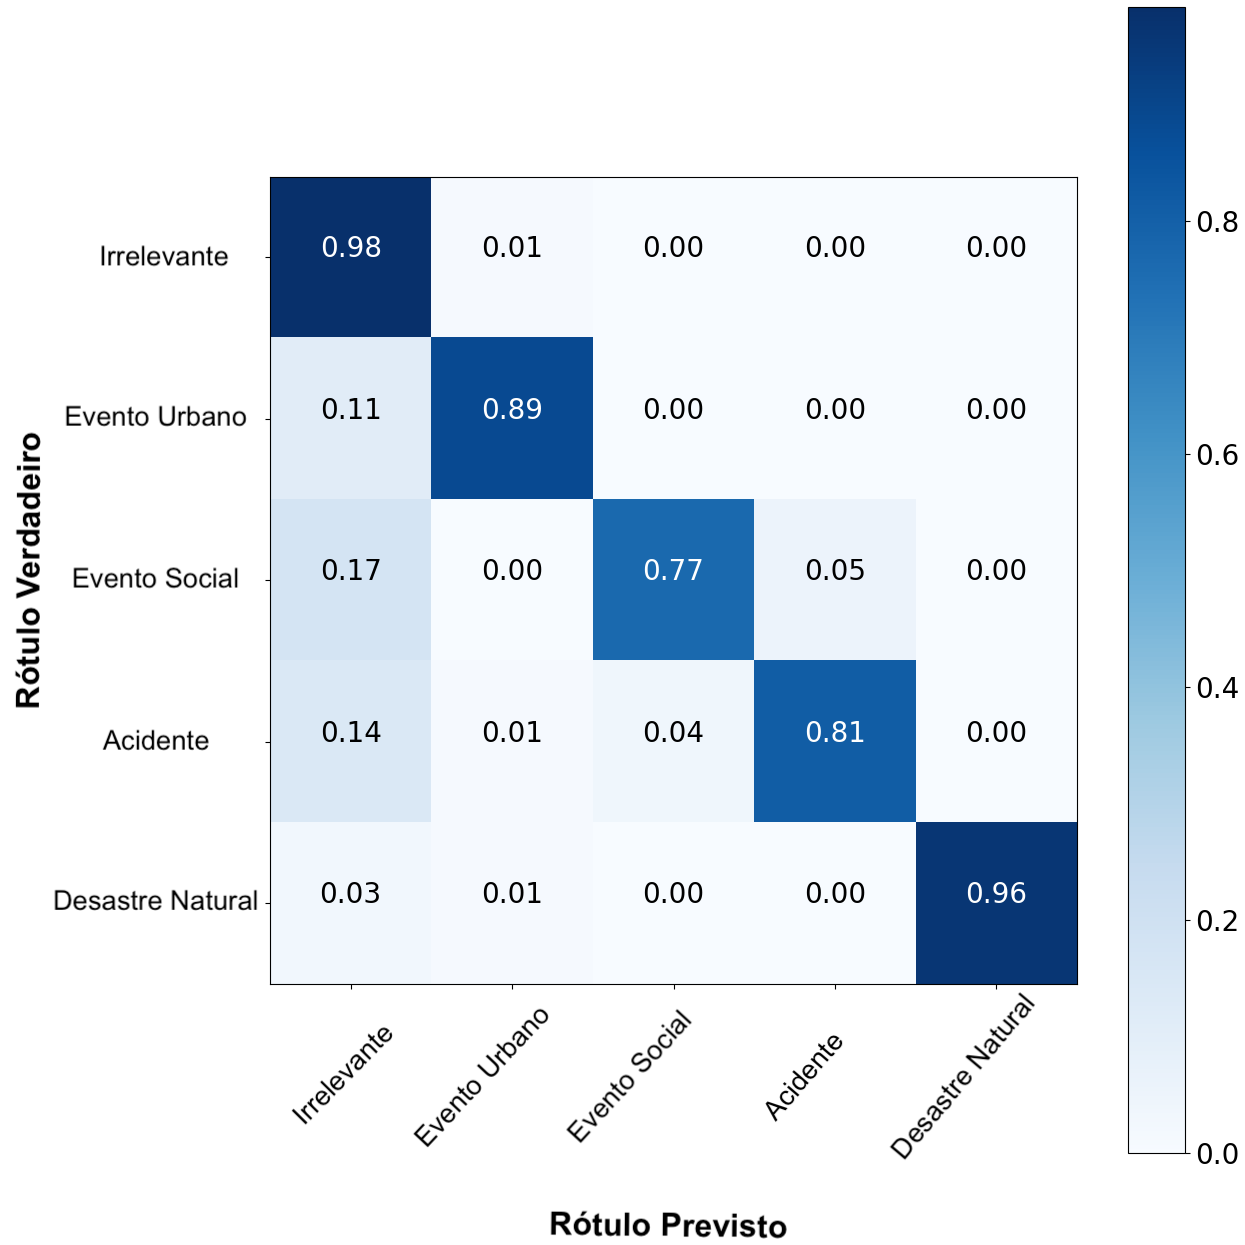
\includegraphics[width=1\linewidth]{images/confusion_matrix_dt_pt.png}
	\label{fig:confusion_matrix_dt}
	\source{Felipe Cordeiro Alves Dias (2019)}
\end{figure}

\begin{figure}[!htb]
	\centering
 	  \caption{Matriz de confusão relacionada a classificação dos \textit{tweets} em eventos de exceção por meio do algoritmo \textit{Naive Bayes} Complementar}
		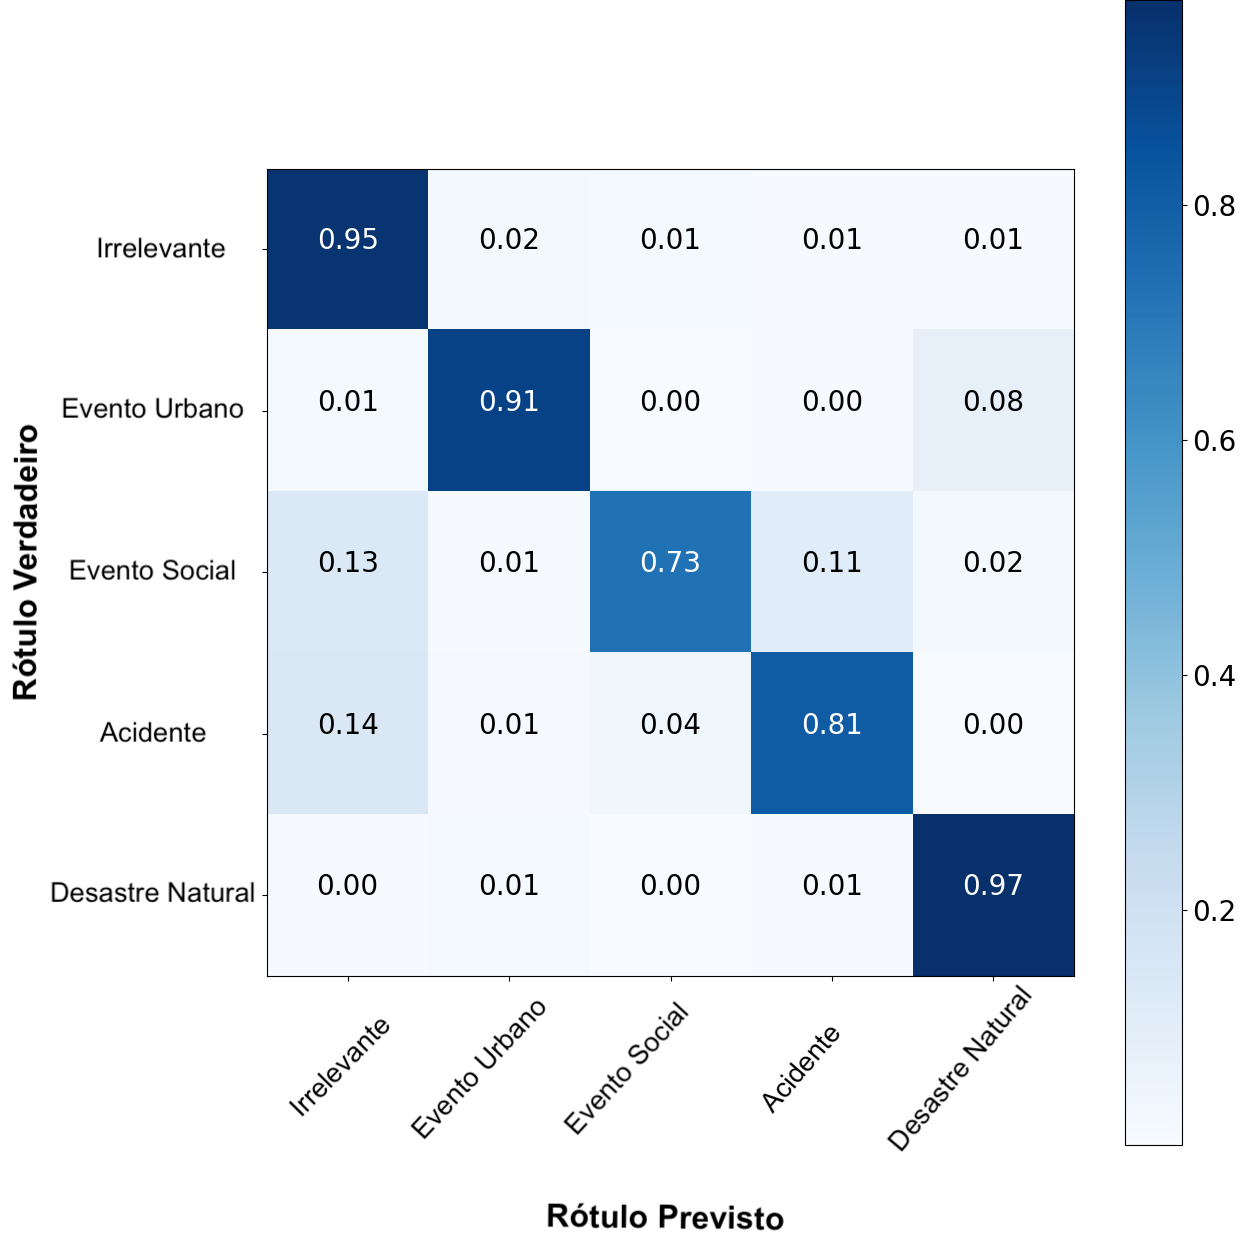
\includegraphics[width=1\linewidth]{images/confusion_matrix_cnb_pt.png}
	\label{fig:confusion_matrix_gnb}
	\source{Felipe Cordeiro Alves Dias (2019)}
\end{figure}

\begin{figure}[!htb]
	\centering
 	  \caption{Matriz de confusão relacionada a classificação dos \textit{tweets} em eventos de exceção por meio do algoritmo Florestas Aleatórias}
		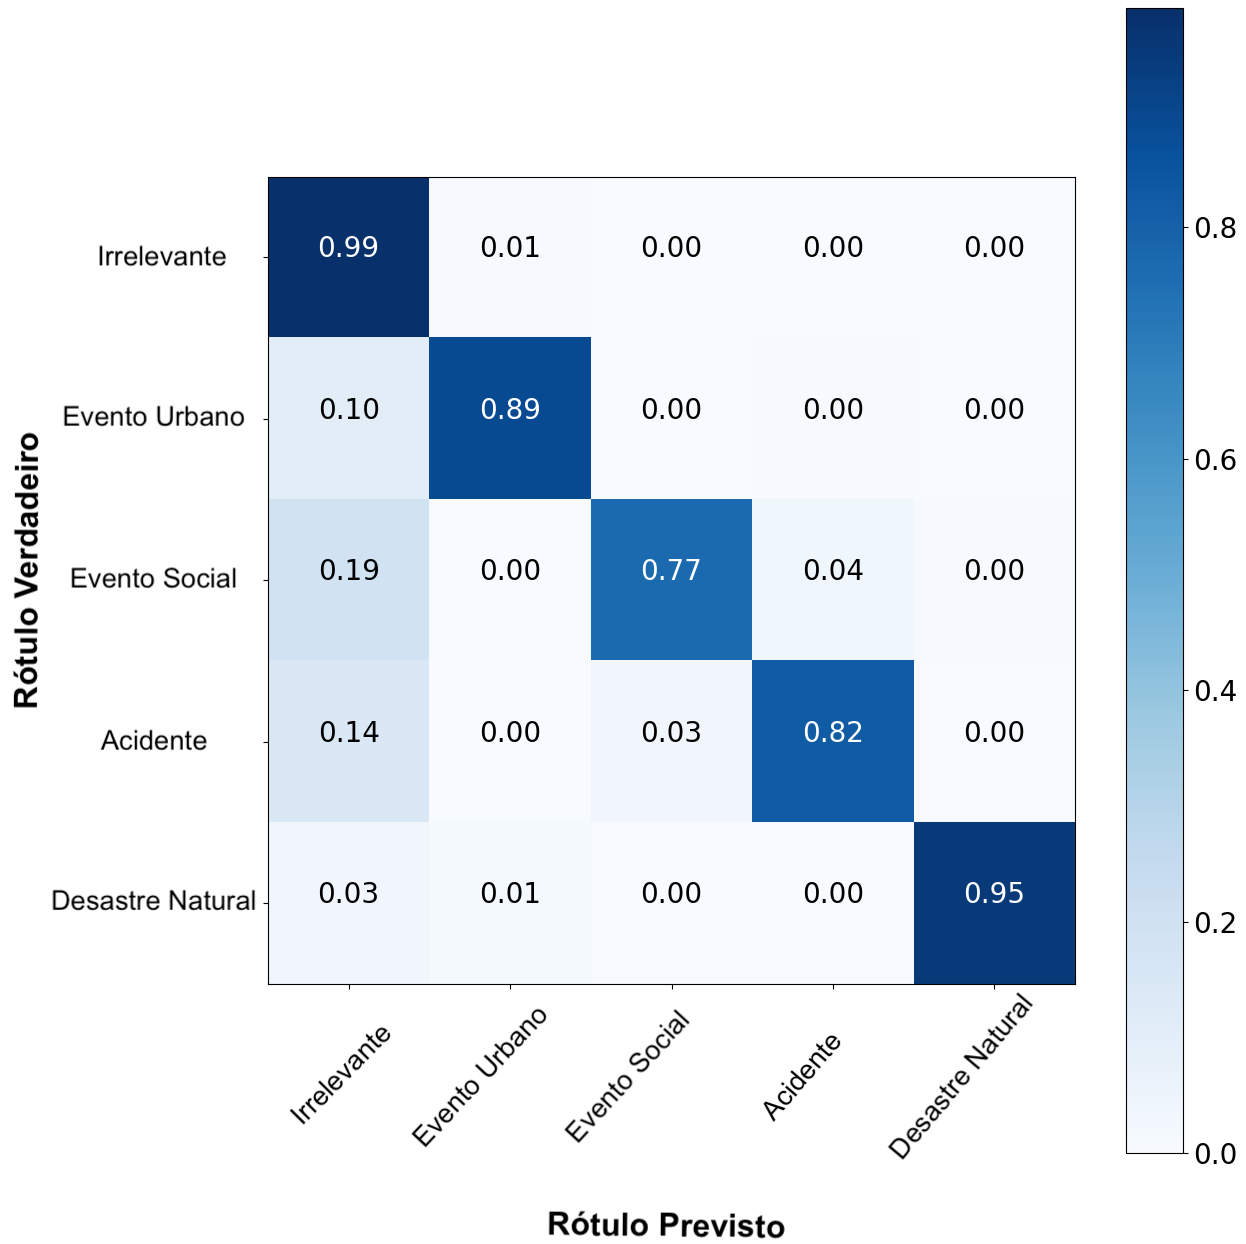
\includegraphics[width=1\linewidth]{images/confusion_matrix_rf_pt.png}
	\label{fig:confusion_matrix_rf}
	\source{Felipe Cordeiro Alves Dias (2019)}
\end{figure}

\begin{figure}[!htb]
	\centering
 	  \caption{Matriz de confusão relacionada a classificação dos \textit{tweets} em eventos de exceção por meio do algoritmo \textit{Naive Bayes} Multinomial}
		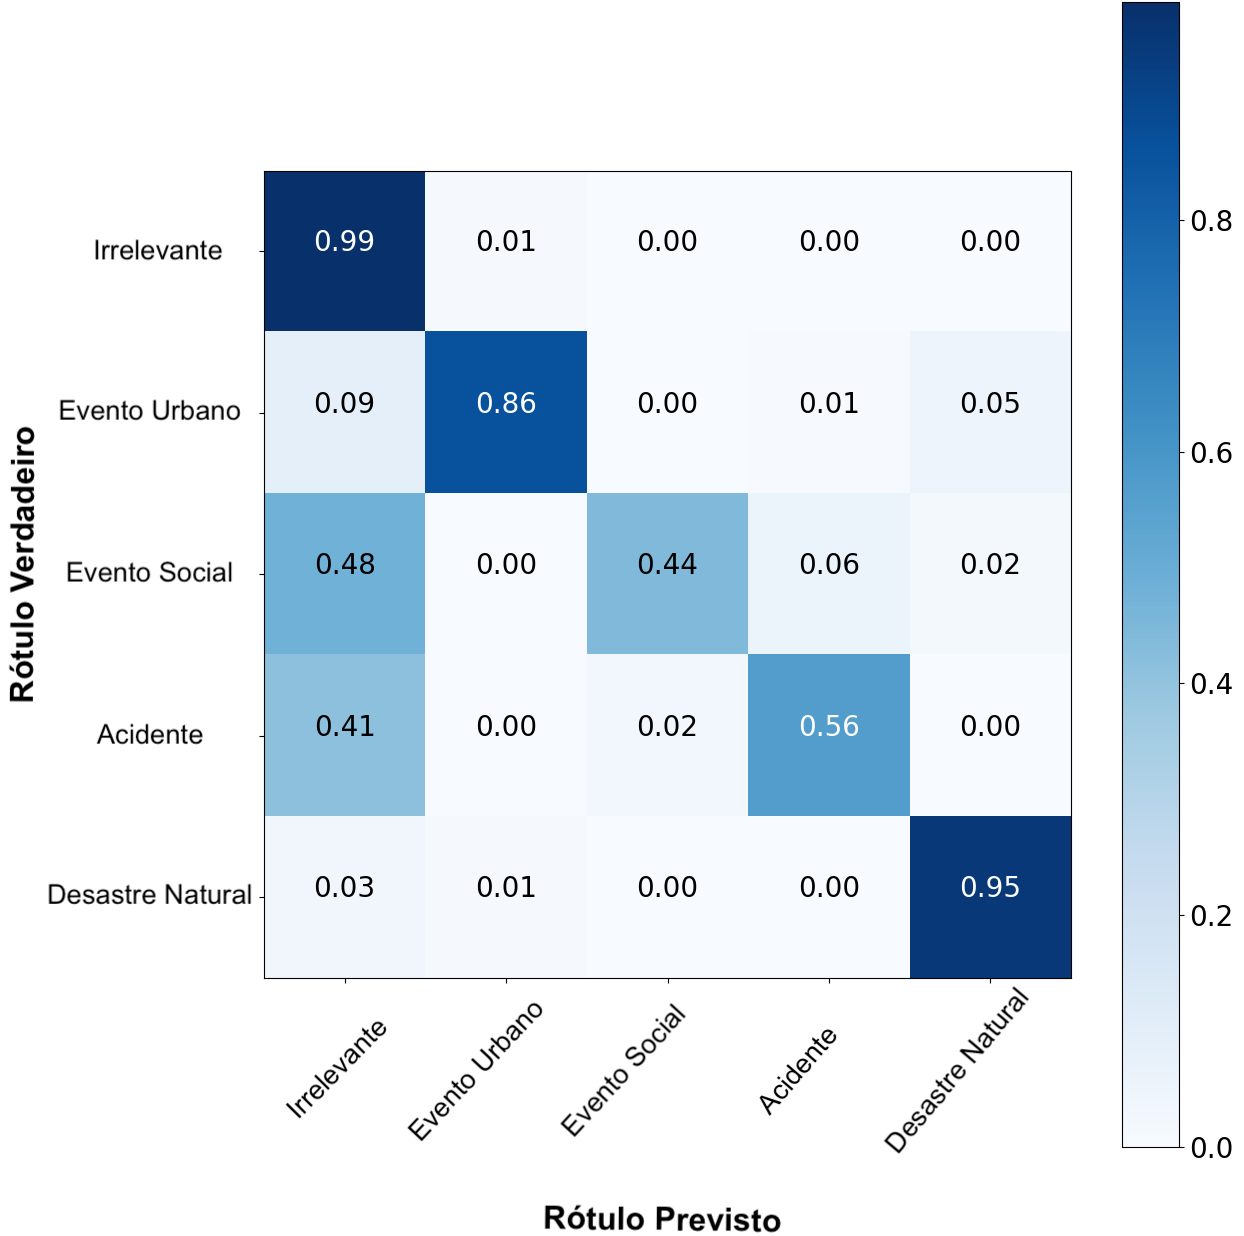
\includegraphics[width=1\linewidth]{images/confusion_matrix_mnb_pt.png}
	\label{fig:confusion_matrix_mnb}
	\source{Felipe Cordeiro Alves Dias (2019)}
\end{figure}

\begin{figure}[!htb]
	\centering
 	  \caption{Matriz de confusão relacionada a classificação dos \textit{tweets} em eventos de exceção por meio do algoritmo Regressão Logística}
		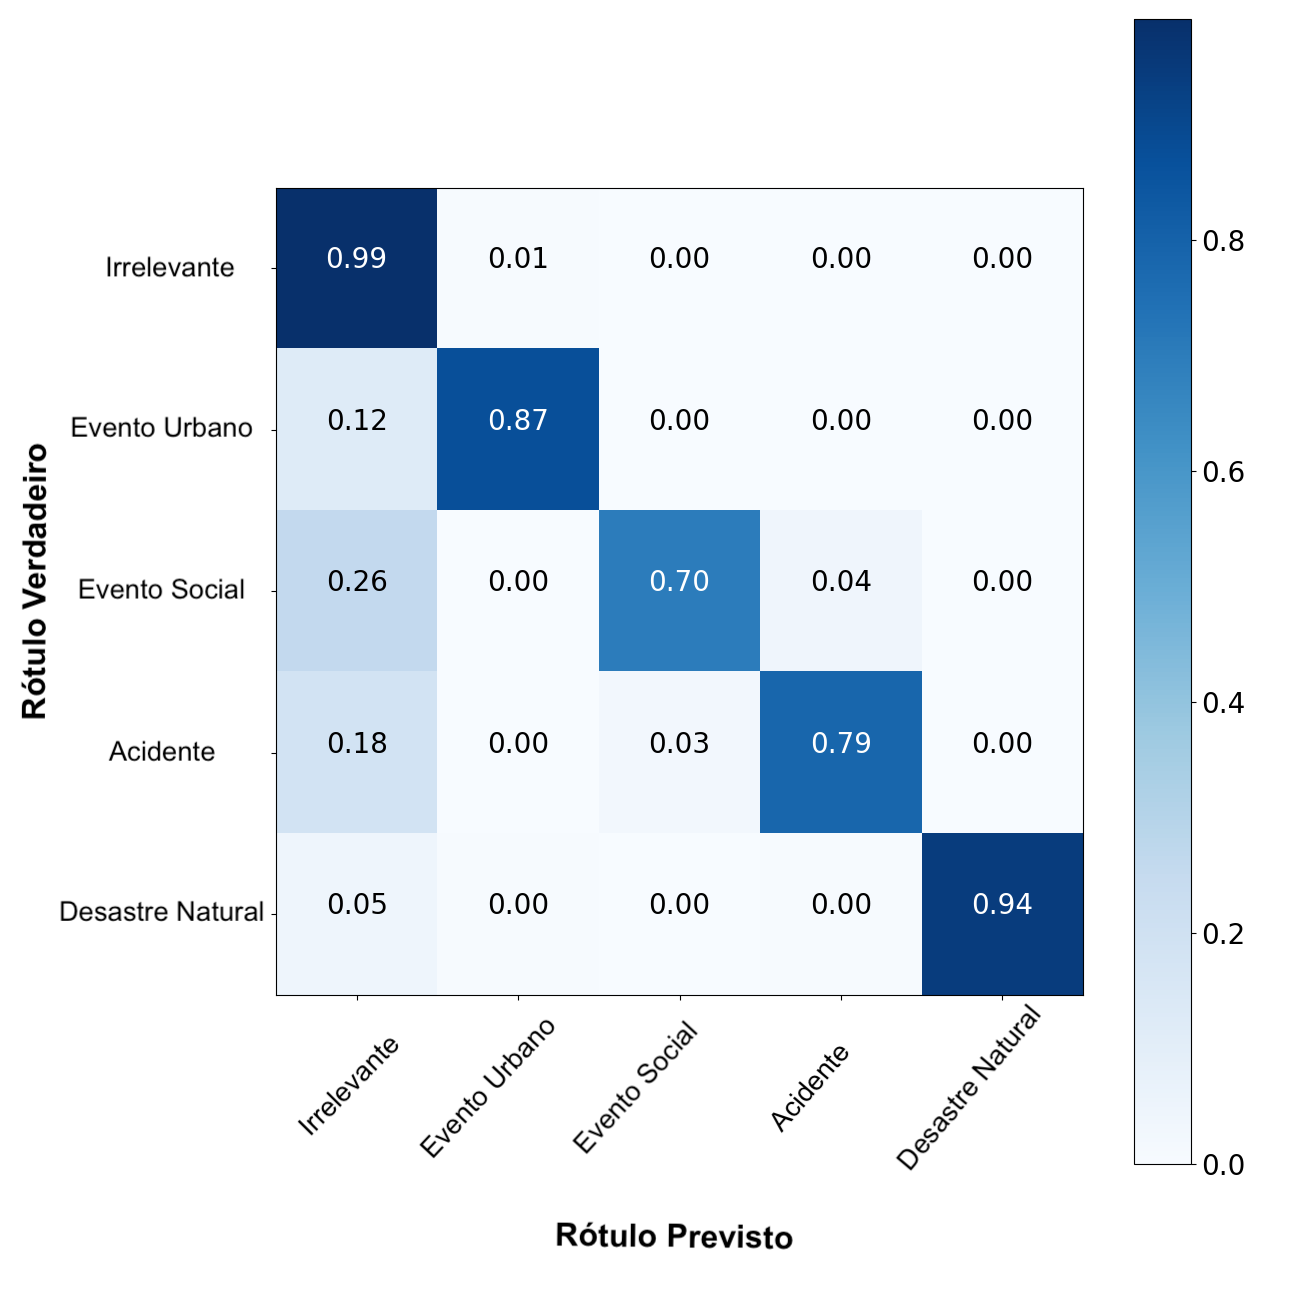
\includegraphics[width=1\linewidth]{images/confusion_matrix_lr_pt.png}
	\label{fig:confusion_matrix_rl}
	\source{Felipe Cordeiro Alves Dias (2019)}
\end{figure}

\begin{figure}[!htb]
	\centering
 	  \caption{Matriz de confusão relacionada a classificação dos \textit{tweets} em eventos de exceção por meio do algoritmo Máquina de Vetores de Suporte}
		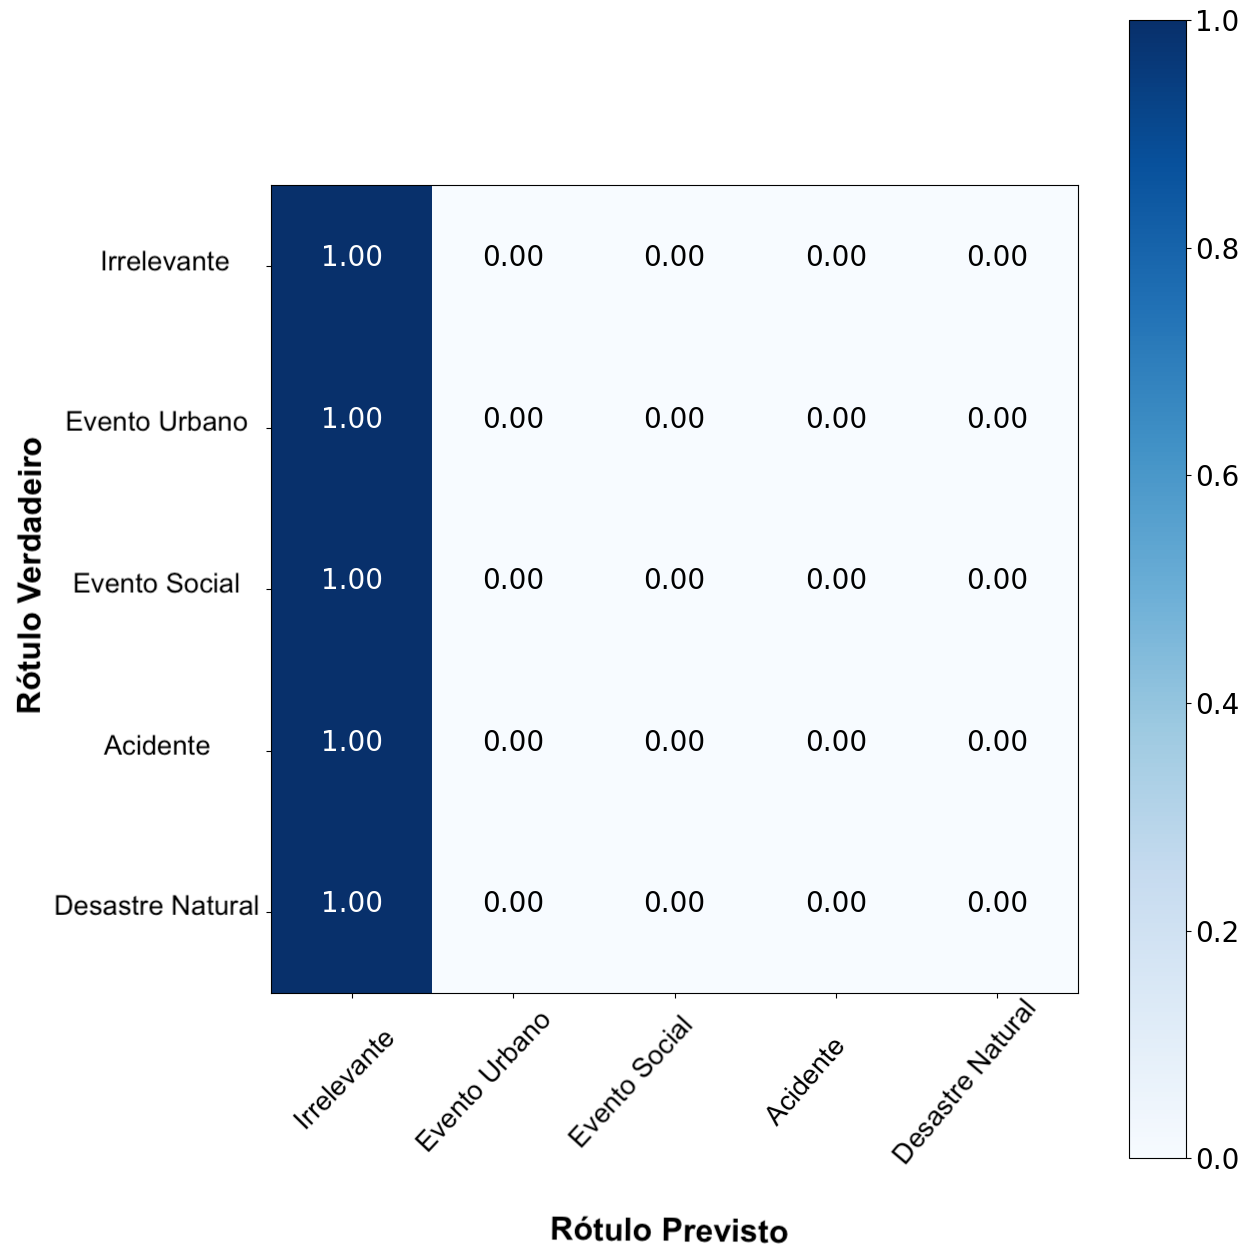
\includegraphics[width=1\linewidth]{images/confusion_matrix_svm_pt.png}
	\label{fig:confusion_matrix_svm}
	\source{Felipe Cordeiro Alves Dias (2019)}
\end{figure}

\chapter{Parametrizações dos algoritmos}
\label{apendiceF}

Neste apêndice estão descritas as parametrizações padrões de cada algoritmo de aprendizado de máquina não supervisionado, utilizados nos experimentos desse trabalho.

\section{Árvore de Decisão}

Abaixo são descritos os parâmetros padrões utilizados para o algoritmo Árvore de Decisão\footnote{Descrições das parametrização adaptadas com base em:\url{http://scikit-learn.org/stable/modules/generated/sklearn.tree.DecisionTreeClassifier.html}. Acesso em 08 de outubro de 2018.}.

\begin{itemize}
\item \textit{criterion} --- $string$, opcional ($default=$\textit{``gini''}) --- Parâmetro responsável por definir a função que mede a qualidade da divisão da árvore de decisão. Os valores suportados são $gini$ para a \textit{impureza Gini} e $entropy$ para o \textit{ganho de informação}.
\item \textit{splitter} --- $string,$ opcional ($default=$\textit{``best''}) --- Parâmetro responsável por definir a estratégia usada para escolher a divisão em cada nó. As estratégias suportadas são $best$ para escolher a melhor divisão e $random$ para escolher a melhor divisão aleatoriamente.
\item \textit{max\_depth} --- $int$ ou $None$, opcional ($default=None$) --- Parâmetro responsável por definir a profundidade máxima da árvore. Se definido como $None$, os nós são expandidos até que todas as folhas fiquem puras ou até que todas as folhas contenham menos amostras que $min\_samples\_split$.
\item \textit{min\_samples\_split} --- $int$, $float$, opcional ($default=2$) --- Parâmetro responsável por definir o número mínimo de amostras necessárias para dividir um nó interno.
\item \textit{min\_samples\_leaf} --- $int$, $float$, opcional ($default=1$) --- Parâmetro responsável por definir o número mínimo de amostras necessárias em um nó folha. Um ponto de divisão em qualquer profundidade só será considerado se deixar pelo menos $min\_samples\_leaf$ amostras de treinamento em cada uma das ramificações esquerda e direita. Isso pode ter o efeito de suavizar o modelo, especialmente na regressão.
\item \textit{min\_weight\_fraction\_leaf} --- $float$, opcional ($default=0.$) --- Parâmetro responsável por definir a fração ponderada mínima da soma total de pesos (de todas as amostras de entrada) necessária para estar em um nó folha. As amostras têm peso igual quando \textit{sample\_weight} não é fornecido.
\item \textit{max\_features} --- $int$, $float$, $string$ ou $None$, opcional ($default=None$) --- Parâmetro responsável por definir o número de \textit{features} (características) a serem consideradas ao procurar a melhor divisão. A procura por uma divisão não é interrompida até que pelo menos uma partição válida das amostras de nó seja localizada, mesmo que seja necessário inspecionar do que mais de \textit{max\_features} características.
\item \textit{random\_state} --- $int$, $RandomState instance$ ou $None$, opcional ($default=None$) --- Parâmetro responsável por determinar a estratégia de geração de número aleatórios. Se definido como $RandomState$, $random\_state$ será o gerador de números aleatórios; se $None$ o gerador de números aleatórios é a instância $RandomState$ usada por $np.random$.
\item \textit{max\_leaf\_nodes} --- $int$ ou $None$, opcional ($default=None$) --- Parâmetro responsável por gerar uma árvore com o máximo número de nós folhas, usando a estratégia \textit{best-first}.
Os melhores (\textit{best}) nós são os definidos como redução relativa a impureza. Caso o parâmetro seja definido como $None$ então o número máximo de nós folhas será ilimitado. 
\item \textit{min\_impurity\_decrease} --- $float$, opcional ($default=0.$) --- Parâmetro responsável por definir que um nó será dividido se essa divisão induzir uma diminuição da impureza maior ou igual a esse valor.
\item \textit{class\_weight} --- $dict$, $list$ de $dict$, ``$balanced$'', $None$, $default=None$ --- Parâmetro responsável por associar ponderação as classes, no seguinte formato: ``${class\_label: weight}$''. Caso não haja valores para esse parâmetro, supõem-se que todos as classes possuam o mesmo peso. 
\item \textit{presort} --- $bool$, opcional ($default=False$) --- Se o valor desse parâmetro é igual a $true$ é realizada uma pré-ordenação dos dados, o que acelera encontrar as melhores divisões das árvores de decisão no processo de ajuste. Ao habilitar esse parâmetro, a velocidade do processo de treinamento de um grande volume de dados  é reduzida. Por outro lado, habilitar esse parâmetro em alguns casos pode acelerar o processo de treinamento, como quando há pequenos conjuntos de dados, ou, restrição quanto a profundidade da árvore de decisão.
\end{itemize}

\section{Floresta Aleatória}

Abaixo são descritos os parâmetros padrões utilizados para o algoritmo Floresta Aleatória\footnote{Descrições das parametrização adaptadas com base em:\url{http://scikit-learn.org/stable/modules/generated/sklearn.ensemble.RandomForestClassifier.html}. Acesso em 08 de outubro de 2018.}.

\begin{itemize}
\item \textit{n\_estimators} --- $integer$, opcional ($default=100$) --- Parâmetro responsável pelo número de árvores na floresta.
\item \textit{criterion} --- $string$, opcional ($default=$\textit{``gini''}) --- Parâmetro responsável por definir a função que mede a qualidade da divisão da árvore de decisão. Os valores suportados são $gini$ para a \textit{impureza Gini} e $entropy$ para o \textit{ganho de informação}.
\item \textit{max\_depth} --- $int$ ou $None$, opcional ($default=None$) --- Parâmetro responsável por definir a profundidade máxima da árvore. Se definido como $None$, os nós são expandidos até que todas as folhas fiquem puras ou até que todas as folhas contenham menos amostras que $min\_samples\_split$.
\item \textit{min\_samples\_split} --- $int$, $float$, opcional ($default=2$) --- Parâmetro responsável por definir o número mínimo de amostras necessárias para dividir um nó interno.
\item \textit{min\_samples\_leaf} --- $int$, $float$, opcional ($default=1$) --- Parâmetro responsável por definir o número mínimo de amostras necessárias em um nó folha. Um ponto de divisão em qualquer profundidade só será considerado se deixar pelo menos $min\_samples\_leaf$ amostras de treinamento em cada uma das ramificações esquerda e direita. Isso pode ter o efeito de suavizar o modelo, especialmente na regressão.
\item \textit{min\_weight\_fraction\_leaf} --- $float$, opcional ($default=0.$) --- Parâmetro responsável por definir a fração ponderada mínima da soma total de pesos (de todas as amostras de entrada) necessária para estar em um nó folha. As amostras têm peso igual quando \textit{sample\_weight} não é fornecido.
\item \textit{max\_features} --- $int$, $float$, $string$ ou $None$, opcional ($default=None$) --- Parâmetro responsável por definir o número de \textit{features} (características) a serem consideradas ao procurar a melhor divisão. A procura por uma divisão não é interrompida até que pelo menos uma partição válida das amostras de nó seja localizada, mesmo que seja necessário inspecionar do que mais de \textit{max\_features} características.
\item \textit{random\_state} --- $int$, $RandomState instance$ ou $None$, opcional ($default=None$) --- Parâmetro responsável por determinar a estratégia de geração de número aleatórios. Se definido como $RandomState$, $random\_state$ será o gerador de números aleatórios; se $None$ o gerador de números aleatórios é a instância $RandomState$ usada por $np.random$.
\item \textit{max\_leaf\_nodes} --- $int$ ou $None$, opcional ($default=None$) --- Parâmetro responsável por gerar uma árvore com o máximo número de nós folhas, usando a estratégia \textit{best-first}.
Os melhores (\textit{best}) nós são os definidos como redução relativa a impureza. Caso o parâmetro seja definido como $None$ então o número máximo de nós folhas será ilimitado. 
\item \textit{min\_impurity\_decrease} --- $float$, opcional ($default=0.$) --- Parâmetro responsável por definir que um nó será dividido se essa divisão induzir uma diminuição da impureza maior ou igual a esse valor.
\item \textit{bootstrap} --- $boolean$, opcional ($default=True$) --- Parâmetro responsável por definir se amostras de \textit{bootstrap} serão usadas ao construir árvores.
\item \textit{oob\_score} --- $boolean$, opcional ($default=False$) --- Parâmetro responsável por definir o uso de amostras \textit{out-of-bag} para estimar a precisão da generalização.
\item \textit{n\_jobs} --- $int$ ou $None$, opcional ($default=None$) --- Parâmetro responsável por definir o número de $jobs$ a serem executados em paralelo durante os processos de \textit{fit} e \textit{predict}. $None$ define 1 \textit{job} a menos que esteja em um contexto \textit{joblib.parallel\_backend}; -1 define que todos os processadores sejam usados.
\item \textit{verbose} --- $int$, opcional ($default=0$) ---
Parâmetro responsável por controlar a verbosidade durante os processos de \textit{fit} e \textit{predict}.
\item \textit{warm\_start} --- $bool$, opcional ($default=False$) --- Parâmetro que
quando definido como $True$ reutiliza a solução da chamada anterior no processo de \textit{fit} e adiciona mais estimadores ao \textit{ensemble}, caso contrário, apenas aplica o processo de \textit{fit} a toda uma nova floresta.
\item \textit{class\_weight} --- $dict$, $list$ de $dict$, ``$balanced$'', $None$, $default=None$ --- Parâmetro responsável por associar ponderação as classes, no seguinte formato: ``${class\_label: weight}$''. Caso não haja valores para esse parâmetro, supõem-se que todos as classes possuam o mesmo peso. 
\item \textit{presort} --- $bool$, opcional ($default=False$) --- Se o valor desse parâmetro é igual a $true$ é realizada uma pré-ordenação dos dados, o que acelera encontrar as melhores divisões das árvores de decisão no processo de ajuste. Ao habilitar esse parâmetro, a velocidade do processo de treinamento de um grande volume de dados  é reduzida. Por outro lado, habilitar esse parâmetro em alguns casos pode acelerar o processo de treinamento, como quando há pequenos conjuntos de dados, ou, restrição quanto a profundidade da árvore de decisão.
\end{itemize}

\section{K-ésimo Vizinho mais Próximo}

Abaixo são descritos os parâmetros padrões utilizados para o algoritmo K-ésimo Vizinho mais Próximo\footnote{Descrições das parametrização adaptadas com base em:\url{http://scikit-learn.org/stable/modules/generated/sklearn.neighbors.KNeighborsClassifier.html}. Acesso em 08 de outubro de 2018.}.

\begin{itemize}

\item \textit{n\_neighbors} --- $int$, opcional ($default = 5$) --- Parâmetro responsável por definir o número padrão de \textit{neighbors} usados pelas \textit{kneighbors queries}.

\item \textit{weights} --- $str$ ou $callable$, opcional ($default = ‘uniform’$) --- Parâmetro usado para definir a função de peso usada no processo \textit{predict}. Valores possíveis: (I) $uniform$: pesos uniformes; todos os pontos em cada vizinha são ponderados igualmente; (II) $distance$: pontos de ponderação pelo inverso da suas respectivas distâncias; nesse caso, os vizinhos mais próximos de um ponto de consulta terão uma influência maior do que os vizinhos mais distantes; (III) $callable$: uma função definida pelo usuário que aceita uma matriz de distâncias e retorna uma matriz da mesma forma, contendo contém os pesos.

\item \textit{algorithm} --- $auto$, $ball\_tree$ (\textit{BallTree}), $kd\_tree$ (\textit{KDTree}), $brute$ (pesquisa por força bruta), opcional ($default = ‘auto’$) --- Parâmetro responsável por definir algoritmo utilizado para calcular os vizinhos mais próximos. O valor padrão tentará decidir o algoritmo mais apropriado com base nos valores passados para o método \textit{fit}. Em case de dados esparsos no processo de ajuste esse parâmetro é ignorado e usado a opção $brute$ por padrão.

\item \textit{leaf\_size} --- $int$, opcional ($default = 30$) --- Parâmetro responsável por definir o tamanho da folha passado para o \textit{BallTree} ou \textit{KDTree}. Isso pode afetar a velocidade da construção e consulta, bem como a memória necessária para armazenar a árvore. O valor ideal depende da natureza do problema.

\item \textit{p} --- $integer$, opcional ($default = 2$) --- Parâmetro de potência para a métrica \textit{Minkowski}. Quando p = 1, isso equivale a usar \textit{manhattan\_distance} ($l1$) e \textit{euclidean\_distance} ($l2$) para p = 2. Para \textit{p} arbitrário, \textit{minkowski\_distance} ($l\_p$) é usado.

\item \textit{metric} --- $string$ ou $callable$, opcional ($default = ‘minkowski’$) --- Parâmetro responsável por definir a distância métrica para usar na árvore. A métrica padrão é \textit{minkowski} e com $p = 2$ é equivalente à métrica euclidiana padrão. 

\item \textit{n\_jobs} --- $int$ ou $None$, opcional ($default = None$) --- Parâmetro responsável por definir o número de $jobs$ a serem executados em paralelo durante os processos de \textit{fit} e \textit{predict}. $None$ define 1 \textit{job} a menos que esteja em um contexto \textit{joblib.parallel\_backend}; -1 define que todos os processadores sejam usados.
\end{itemize}

\section{Máquina de Vetores de Suporte}

Abaixo são descritos os parâmetros padrões utilizados para o algoritmo Máquina de Vetores de Suporte
\footnote{Descrições das parametrização adaptadas com base em:\url{http://scikit-learn.org/stable/modules/generated/sklearn.svm.SVC.html\#sklearn.svm.SVC}. Acesso em 08 de outubro de 2018.}.

\begin{itemize}
\item \textit{C} --- $float$, opcional ($default=1.0$)
 --- Parâmetro de \textit{penalidade C} do termo de erro.
 
 \item \textit{kernel} --- $string$, opcional ($default='rbf'$) --- Parâmetro responsável por especificar o tipo de \textit{kernel} a ser usado no algoritmo. Pode ser $linear$, $poli$, $rbf$, $sigmoid$, $precomputed$ ou $callable$.

\item \textit{degree} --- $int$, opcional ($default=3$) --- Parâmetro responsável por definir a \textit{polynomial kernel function} ($poly$). Ignorado por todos os 
outros \textit{kernels}.

\item \textit{gamma} --- $float$, opcional ($default='auto'$) --- Parâmetro responsável por definir o coeficiente de \textit{Kernel} para $rbf$, $poly$ e $sigmoid$.

\item \textit{coef0} --- $float$, opcional ($default=0.0$) --- Parâmetro responsável por definir o termo independente na função \textit{kernel}. É significativo apenas para $poli$ e $sigmoid$.

\item \textit{shrinking} --- $boolean$, opcional ($default=True$) --- Parâmetro responsável por definir o uso da heurística $shrinking$.

\item \textit{probability} --- $boolean$, opcional ($default=False$) --- Parâmetro responsável por definir o uso de estimativas de probabilidade, o qual deve ser ativado antes do processo de $fit$ (implica em perda de desempenho).

\item \textit{tol} --- $float$, opcional ($default=1e-3$) --- Parâmetro responsável por definir a tolerância ao critério de parada.

\item \textit{cache\_size} --- $float$, opcional --- Parâmetro responsável por definir o tamanho do cache do \textit{kernel} (em MB).

\item \textit{class\_weight} --- $dict$, $balanced$, optional ($default = None$) --- Parâmetro responsável  por definir o parâmetro C da classe $i$ para $class\_weight[i]*C$ para o \textit{SVC}.

\item \textit{verbose} --- $bool$, ($default = False$) --- Parâmetro responsável por habilitar a saída detalhada.

\item \textit{max\_iter} --- $int$, opcional ($default=-1$) --- Parâmetro responsável por definir um limite rígido em iterações no \textit{solver}, ou -1 para sem limite.

\item \textit{decision\_function\_shape} --- $ovo$, $ovr$, ($default='ovr'$) --- Parâmetro responsável por definir se deve retornar uma função de decisão \textit{one-vs-rest} ($ovr$) ou a função de decisão original \textit{one-vs-one}.

\item \textit{random\_state} --- $int$, $RandomState instance$ ou $None$, opcional ($default=None$) --- Parâmetro responsável por determinar a estratégia de geração de número aleatórios. Se definido como $RandomState$, $random\_state$ será o gerador de números aleatórios; se $None$ o gerador de números aleatórios é a instância $RandomState$ usada por $np.random$.

\end{itemize}

\section{Naive Bayes}

Abaixo são descritos os parâmetros padrões utilizados para o algoritmo Naive Bayes\footnote{Descrições das parametrização adaptadas com base em:\url{http://scikit-learn.org/stable/modules/generated/sklearn.naive_bayes.MultinomialNB.html\#sklearn.naive_bayes.MultinomialNB} e \url{http://scikit-learn.org/stable/modules/generated/sklearn.naive_bayes.ComplementNB.html\#sklearn.naive_bayes.ComplementNB} . Acesso em 08 de outubro de 2018.}.

\begin{itemize}
\item \textit{alpha} --- $float$, opcional ($default=1.0$) --- Parâmetro de suavização (0 para não suavização) aditivo (Laplace / Lidstone).
\item \textit{fit\_prior} --- $boolean$, opcional ($default=True$) --- Parâmetro responsável por definir ou não o aprendizado das probabilidades anteriores da classe.
\item \textit{class\_prior} --- $array-like$, $size$ ($n\_classes$,), opcional ($default=None$) --- Parâmetro responsável por definir probabilidades anteriores das classes. Se especificado, os antecedentes não são ajustados de acordo com os dados.
\item \textit{norm} --- $boolean$, opcional ($default=False$) ---
Parâmetro responsável por definir se uma segunda normalização dos pesos é executada ou não. Disponível somente na implementação \textit{ComplementNB}.
\end{itemize}

\section{Perceptron Multicamadas}

Abaixo são descritos os parâmetros padrões utilizados para o algoritmo Perceptron Multicamadas\footnote{Descrições das parametrização adaptadas com base em:\url{http://scikit-learn.org/stable/modules/generated/sklearn.neural_network.MLPClassifier.html\#sklearn.neural_network.MLPClassifier}. Acesso em 08 de outubro de 2018.}.

\begin{itemize}
\item\textit{hidden\_layer\_sizes} --- $tuple$, $length = n\_layers - 2$,  opcional($default = (100,)$) --- Parâmetro responsável por definir o $ith$ elemento que representa o número de neurônios na $ith$ camada oculta.
\item \textit{activation} --- $identity$, $logistic$, $tanh$, $relu$, opcional ($default =relu$) --- Parâmetro responsável por definir a função de ativação para a camada oculta.
\item \textit{solver} --- $lbfgs$, $sgd$, $adam$, opcional ($default = adam$) --- Parâmetro responsável por definir o solucionador para otimização de peso.
\item \textit{alpha} --- $float$, opcional ($default=0.0001$) --- Parâmetro de penalidade L2 (termo de regularização).
\item \textit{batch\_size} --- $int$, opcional ($default = auto$) --- Parâmetro responsável pelo tamanho de \textit{mini-batches} para otimizadores estocásticos. Se o solucionador for $lbfgs$, o classificador não usa $minibatch$. Quando definido como $auto$, $batch\_size = min (200, n_samples)$.
\item \textit{learning\_rate} --- $constant$, $invscaling$, $adaptive$,opcional ($default$ = $constant$) --- Parâmetro responsável pela programação da taxa de aprendizado para atualizações de ponderações.
\item \textit{learning\_rate\_init} --- $double$, opcional ($default = 0.001$) --- Parâmetro responsável por definir a taxa inicial de aprendizado utilizada, somente quando $solver = sgd$ ou $adam$.
\item \textit{power\_t} --- $double$, opcional ($default = 0.5$) --- Parâmetro responsável por definir o expoente para a taxa de aprendizado de escala inversa, quando a \textit{learning\_rate} é definida como $invscaling$ e $solver = sgd$. 
\item \textit{max\_iter} --- $int$, opcional ($default = 200$) --- Parâmetro responsável por definir o número máximo de iterações. O \textit{solver} itera até a convergência (determinada por \textit{tol}) ou pelo \textit{max\_iter}. Para \textit{solvers} estocásticos ($sgd$, $adam$), esse parâmetro determina o número de \textit{epochs} (quantas vezes cada ponto de dados será usado), não o número de etapas do gradiente.
\item \textit{shuffle} --- $bool$, opcional ($default = True$) --- Parâmetro responsável por definir o embaralhamento das amostras em cada iteração. Usado somente quando $solver = sgd$ ou $adam$.
\item \textit{random\_state} --- $int$, $RandomState instance$ ou $None$, opcional ($default=None$) --- Parâmetro responsável por determinar a estratégia de geração de número aleatórios. Se definido como $RandomState$, $random\_state$ será o gerador de números aleatórios; se $None$ o gerador de números aleatórios é a instância $RandomState$ usada por $np.random$.
\item \textit{verbose} --- $bool$, ($default = False$) --- Parâmetro responsável por habilitar a saída detalhada.
\item \textit{tol} --- $float$, opcional, ($default=1e-4$) --- Parâmetro responsável por definir a tolerância para a otimização.
\item \textit{warm\_start} --- $bool$, opcional ($default=False$) --- Parâmetro responsável por definir a reutilização da solução da chamada anterior para o processo de \textit{fit} como inicialização, caso contrário, a solução anterior é apagada.
\item \textit{momentum} --- $float$, opcional ($default=0.9$) --- Parâmetro responsável por definir o \textit{momentum} para a atualização de descida de gradiente. Deve estar entre 0 e 1. Apenas utilizado quando $solver=sgd$.
\item \textit{nesterovs\_momentum} --- $boolean$, ($default=True$) --- Parâmetro responsável por definir o uso do \textit{Nesterov’s momentum}. Apenas utilizando quando $solver=sgd$ e $momentum > 0$.
\item \textit{early\_stopping} --- $bool$, opcional ($default=False$) --- Parâmetro responsável por definir parada antecipada para finalizar o treinamento quando a pontuação de validação não estiver melhorando. Se definido como verdadeiro,  automaticamente 10\% dos dados de treinamento são usados como validação,  encerrando o treinamento quando a pontuação de validação não estiver melhorando em pelo menos $tol$ para \textit{n\_iter\_no\_change} \textit{epochs} consecutivos. Esse parâmetro somente é efetivo quando $solver=sgd$ ou $adam$.
\item \textit{validation\_fraction} --- $float$, opcional, ($default=0.1$) --- Parâmetro responsável por definir a proporção de dados de treinamento a serem definidos como um conjunto de validação para interrupção antecipada. O valor deve estar entre 0 e 1. Apenas usado se $early\_stopping=True$.
\item \textit{beta\_1} --- $float$, opcional ($default=0.9$) --- Parâmetro responsável por definir a taxa de decaimento exponencial (entre 0 e 1) para estimativas do primeiro momento vetorial em \textit{adam}. Usado somente quando $solver=adam$.
\item \textit{beta\_2} --- $float$, opcional ($default=0.9$) --- Parâmetro responsável por definir a taxa de decaimento exponencial (entre 0 e 1) para estimativas do segundo momento vetorial em \textit{adam}. Usado somente quando $solver=adam$.
\item \textit{epsilon} --- $float$, opcional ($default=1e-8$) --- Parâmetro responsável por definir o valor para estabilidade numérica em \textit{adam}. Usado somente quando $solver=adam$.
\item \textit{n\_iter\_no\_change} --- $int$, opcional ($default=10$) --- Parâmetro responsável por definir o número máximo de \textit{epochs} para não atender a melhoria definida pelo parâmetro \textit{tol}. Usado somente quando $solver=adam$.
\end{itemize}

\section{Regressão Logística}

Abaixo são descritos os parâmetros padrões utilizados para o algoritmo Regressão Logística\footnote{Descrições das parametrização adaptadas com base em:\url{http://scikit-learn.org/stable/modules/generated/sklearn.linear_model.LogisticRegression.html}. Acesso em 08 de outubro de 2018.}.

\begin{itemize}
\item \textit{penalty} --- $str$, $l1’$ ou $l2$, opcional ($default=l2$) --- Usado para especificar a norma usada na penalização. Os solucionadores "newton-cg", "sag" e "lbfgs" apoiam apenas as penalidades l2.
\item \textit{dual} --- $bool$, opcional ($default=False$) --- Parâmetro responsável por definir formulação \textit{dual} ou \textit{primal}. Formulação \textit{dual} é apenas implementada para penalidade $l2$ com o $liblinear solver$. Preferível $dual=False$ quando $n\_samples > n\_features$.
\item \textit{tol} --- $float$, opcional ($default=1e-4$) --- Parâmetro responsável por definir a tolerância para o critério de parada.
\item \textit{C}  --- $float$, opcional ($default=1.0$) --- Parâmetro responsável por definir a inversão da força de regularização; deve ser um \textit{floar} positivo. Como nas máquinas de vetores de suporte, valores menores especificam uma regularização mais forte.
\item \textit{fit\_intercept} --- $bool$, opcional ($default=True$) --- Parâmetro responsável por definir se uma constante (viés ou interceptação) deve ser adicionada a função de decisão.
\item \textit{intercept\_scaling} --- $float$, opcional ($default=1$) --- Parâmetro responsável por definir a escala de interceptação. Útil somente quando $solver=liblinear$ e $self.fit_intercept=True$.
\item \textit{class\_weight} --- $dict$, $list$ de $dict$, ``$balanced$'', $None$, $default=None$ --- Parâmetro responsável por associar ponderação as classes, no seguinte formato: ``${class\_label: weight}$''. Caso não haja valores para esse parâmetro, supõem-se que todos as classes possuam o mesmo peso. 
\item \textit{random\_state} --- $int$, $RandomState instance$ ou $None$, opcional ($default=None$) --- Parâmetro responsável por determinar a estratégia de geração de número aleatórios. Se definido como $RandomState$, $random\_state$ será o gerador de números aleatórios; se $None$ o gerador de números aleatórios é a instância $RandomState$ usada por $np.random$.
\item $solver$ --- $str$, $newton-cg$, $lbfgs$, $liblinear$, $sag$, $saga$, opcional ($default=liblinear$) --- Parâmetro responsável por definir o algoritmo utilizado no problema de otimização.
\item \textit{max\_iter} --- $int$, opcional ($default=100$) --- Parâmetro utilizado com $solver=newton-cg$, $sag$ e $lbfgs$. Número máximo de iterações tomadas para os \textit{solvers} convergirem.
\item \textit{verbose} --- $bool$, ($default = False$) --- Parâmetro responsável por habilitar a saída detalhada.
\item \textit{multi\_class} --- $str$, $ovr$, $multinomial$, $auto$, opcional ($default=ovr$) --- Parâmetro responsável por definir multi classes.
\item \textit{warm\_start} --- $bool$, opcional ($default=False$) --- Parâmetro que quando definido como $True$, reutiliza a solução da chamada anterior para o processo de \textit{fit} como inicialização, caso contrário, a solução anterior é apagada. Sem efeitos quando $solver=liblinear$.
\item \textit{n\_jobs} --- $int$ ou $None$, opcional ($default=None$) --- Parâmetro responsável por definir a quantidade de núcleos de CPU utilizados na paralelização sob as classes, quando $multi\_class=ovr$. Esse parâmetro é ignorado quando $solver=liblinear$, independentemente de $multi\_class$ estar especificado ou não. $None$ define 1 núcleo a menos que esteja em um contexto $joblib.parallel_backend$; -1 define o uso de todos os processadores.
\end{itemize}

%solver : str, {‘newton-cg’, ‘lbfgs’, ‘liblinear’, ‘sag’, ‘saga’}, default: ‘liblinear’.
%Algorithm to use in the optimization problem.
%For small datasets, ‘liblinear’ is a good choice, whereas ‘sag’ and ‘saga’ are faster for large ones.
%For multiclass problems, only ‘newton-cg’, ‘sag’, ‘saga’ and ‘lbfgs’ handle multinomial loss; ‘liblinear’ is limited to one-versus-rest schemes.
%‘newton-cg’, ‘lbfgs’ and ‘sag’ only handle L2 penalty, whereas ‘liblinear’ and ‘saga’ handle L1 penalty.
%Note that ‘sag’ and ‘saga’ fast convergence is only guaranteed on features with approximately the same scale. You can preprocess the data with a scaler from sklearn.preprocessing.
%New in version 0.17: Stochastic Average Gradient descent solver.
%New in version 0.19: SAGA solver.
%Changed in version 0.20: Default will change from ‘liblinear’ to ‘lbfgs’ in 0.22.
%max_iter : int, default: 100
%Useful only for the newton-cg, sag and lbfgs solvers. Maximum number of iterations taken for the solvers to converge.
%multi_class : str, {‘ovr’, ‘multinomial’, ‘auto’}, default: ‘ovr’
%If the option chosen is ‘ovr’, then a binary problem is fit for each label. For ‘multinomial’ the loss minimised is the multinomial loss fit across the entire probability distribution, even when the data is binary. ‘multinomial’ is unavailable when solver=’liblinear’. ‘auto’ selects ‘ovr’ if the data is binary, or if solver=’liblinear’, and otherwise selects ‘multinomial’.
%New in version 0.18: Stochastic Average Gradient descent solver for ‘multinomial’ case.
%Changed in version 0.20: Default will change from ‘ovr’ to ‘auto’ in 0.22.
%verbose : int, default: 0
%For the liblinear and lbfgs solvers set verbose to any positive number for verbosity.
%warm_start : bool, default: False
%When set to True, reuse the solution of the previous call to fit as initialization, otherwise, just erase the previous solution. Useless for liblinear solver. See the Glossary.
%New in version 0.17: warm_start to support lbfgs, newton-cg, sag, saga solvers.
%n_jobs : int or None, optional (default=None)
%Number of CPU cores used when parallelizing over classes if multi_class=’ovr’”. This parameter is ignored when the solver is set to ‘liblinear’ regardless of whether ‘multi_class’ is specified or not. None means 1 unless in a joblib.parallel_backend context. -1 means using all processors. See Glossary for more details.

\chapter{Análise \textit{Apriori}}
\label{apendiceG}

Neste apêndice, detalhamos as regras de associação encontradas na base de dados AVL, por meio do algoritmo \textit{Apriori}.

\section{Análise \textit{Apriori} aplicada as velocidades médias (intervalos de 5 minutos) ao conjunto de dados AVL da SPTrans, referentes aos meses do ano de 2017.}
\label{g1}

\begin{table}[!htb]
\centering
\caption {Análise \textit{Apriori} aplicada as velocidades médias (intervalos de 5 minutos) ao conjunto de dados AVL da SPTrans --- Referente ao mês de Janeiro}
\label {tab:aprioriJanuary}
\begin{tabular}{c|c|c|c}
\toprule
\textbf{Regra de associação} & \textit{\textbf{Support}} & \textit{\textbf{Confidence}} & \textit{\textbf{Lift}} \\
\midrule
10 &  0,14 &  0,14 &  1\\
\hline
11 &  0,28 &  0,28 &  1\\
\hline
12 &  0,27 &  0,27 &  1\\
\hline
13 &  0,15 &  0,15 &  1\\
\hline
2 &  0,12 &  0,12&  1\\
\hline
4 &  0,10&  0,10 &  1\\
\hline
5 &  0,11 &  0,11 &  1\\
\hline
6 &  0,12 &  0,12 &  1\\
\hline
7 &  0,19 &  0,19 &  1\\
\hline
8 &  0,15 &  0,15&  1\\
\hline
9 &  0,13 &  0,13 &  1\\
\hline
11 $\rightarrow$ 12 &  0,13 &  0,47&  1,72\\
\bottomrule
\end{tabular}
\source{Felipe Cordeiro Alves Dias (2019)}
\end{table}

\begin{table}[!htb]
\centering
\caption {Análise \textit{Apriori} aplicada as velocidades médias (intervalos de 5 minutos) ao conjunto de dados AVL da SPTrans --- Referente ao mês de Fevereiro}
\label {tab:aprioriFebruary}
\begin{tabular}{c|c|c|c}
\toprule
\textbf{Regra de associação} & \textit{\textbf{Support}} & \textit{\textbf{Confidence}} & \textit{\textbf{Lift}} \\
\midrule
10 &  0,17 &  0,17 &  1\\
 \hline 
 11 &  0,21 &  0,21 &  1\\ 
 \hline 
 12 &  0,32 &  0,32 &  1\\ 
 \hline 
 13 &  0,19 &  0,19&  1\\ 
 \hline 
 14 &  0,10 &  0,10 &  1\\ 
 \hline 
 2 &  0,12 &  0,12 &  1\\ 
 \hline 
 5 &  0,12 &  0,12 &  1\\ 
 \hline 
 6 &  0,10 &  0,10 &  1\\ 
 \hline 
 7 &  0,20 &  0,20 &  1\\ 
 \hline 
 8 &  0,13 &  0,13 &  1\\ 
 \hline 
 9 &  0,18 &  0,18 &  1\\
  \hline 
 12 $\rightarrow$ 11 &  0,12 &  0,58 &  1,77\\ 
 \hline 
 12 $\rightarrow$ 13 &  0,12 &  0,37 &  1,95\\ 
 \hline 7 $\rightarrow$ 8 &  0,10 &  0,49 &  3,58\\
\bottomrule
\end{tabular}
\source{Felipe Cordeiro Alves Dias (2019)}
\end{table}

\begin{table}[!htb]
\centering
\caption {Análise \textit{Apriori} aplicada as velocidades médias (intervalos de 5 minutos) ao conjunto de dados AVL da SPTrans --- Referente ao mês de Março}
\label {tab:aprioriMarch}
\begin{tabular}{c|c|c|c}
\toprule
\textbf{Regra de associação} & \textit{\textbf{Support}} & \textit{\textbf{Confidence}} & \textit{\textbf{Lift}} \\
\midrule 
10 &  0,15 &  0,15 &  1\\ 
\hline 
11 &  0,21 &  0,21 &  1\\ 
\hline 
12 &  0,38 &  0,38 &  1\\ 
\hline 
13 &  0,23 &  0,23 &  1\\ 
\hline 
14 &  0,13 &  0,13 &  1\\ 
\hline 
2 &  0,12 &  0,12 &  1\\ 
\hline 
5 &  0,12 &  0,12 &  1\\ 
\hline 
6 &  0,10 &  0,10 &  1\\ 
\hline 
7 &  0,17 &  0,17 &  1\\ 
\hline 
9 &  0,16 &  0,16 &  1\\ 
\hline 
12 $\rightarrow$ 11 &  0,13 &  0,62 &  1,62\\ 
\hline 
12 $\rightarrow$ 13 &  0,15 &  0,41 &  1,76\\
\bottomrule
\end{tabular}
\source{Felipe Cordeiro Alves Dias (2019)}
\end{table}


\begin{table}[!htb]
\centering
\caption {Análise \textit{Apriori} aplicada as velocidades médias (intervalos de 5 minutos) ao conjunto de dados AVL da SPTrans --- Referente ao mês de Abril}
\label {tab:aprioriApril}
\begin{tabular}{c|c|c|c}
\toprule
\textbf{Regra de associação} & \textit{\textbf{Support}} & \textit{\textbf{Confidence}} & \textit{\textbf{Lift}} \\
\midrule 
10 &  0,125 &  0,12 &  1\\
\hline
11 &  0,20 &  0,20 &  1\\
\hline
12 &  0,29 &  0,29 &  1\\
\hline
13 &  0,16 &  0,16 &  1\\
\hline
2 &  0,12 &  0,12 &  1\\
\hline
4 &  0,12 &  0,12 &  1\\
\hline
5 &  0,11 &  0,11 &  1\\
\hline
6 &  0,10 &  0,10 &  1\\
\hline
7 &  0,23 &  0,23 &  1\\
\hline
8 &  0,14 &  0,14 &  1\\
\hline
9 &  0,16 &  0,16 &  1\\
\hline
12  $\rightarrow$ 11 &  0,12 &  0,60 &  2,01\\
\hline
13  $\rightarrow$ 12 &  0,10 &  0,36&  2,28\\
\hline
7  $\rightarrow$ 8 &  0,10 &  0,45 &  3,18\\
\bottomrule
\end{tabular}
\source{Felipe Cordeiro Alves Dias (2019)}
\end{table}

\begin{table}[!htb]
\centering
\caption {Análise \textit{Apriori} aplicada as velocidades médias (intervalos de 5 minutos) ao conjunto de dados AVL da SPTrans --- Referente ao mês de Maio}
\label {tab:aprioriMay}
\begin{tabular}{c|c|c|c}
\toprule
\textbf{Regra de associação} & \textit{\textbf{Support}} & \textit{\textbf{Confidence}} & \textit{\textbf{Lift}} \\
\midrule
10 &  0,11 &  0,11 &  1\\
\hline
11 &  0,21 &  0,21 &  1\\
\hline
12 &  0,37 &  0,37 &  1\\
\hline
13 &  0,21 &  0,21 &  1\\
\hline
14 &  0,12 &  0,12 &  1\\
\hline
2 &  0,12 &  0,12 &  1\\
\hline
5 &  0,12 &  0,12 &  1\\
\hline
6 &  0,11 &  0,11 &  1\\
\hline
7 &  0,19 &  0,19 &  1\\
\hline
8 &  0,13 &  0,13 &  1\\
\hline
9 &  0,15 &  0,15 &  1\\
\hline
12 $\rightarrow$ 11 &  0,13 &  0,64 &  1,70\\
\hline
13 $\rightarrow$ 12 &  0,16 &  0,42 &  1,94\\
\hline
7 $\rightarrow$ 8 &  0,10 &  0,57 &  4,37\\
\bottomrule
\end{tabular}
\source{Felipe Cordeiro Alves Dias (2019)}
\end{table}

\begin{table}[!htb]
\centering
\caption {Análise \textit{Apriori} aplicada as velocidades médias (intervalos de 5 minutos) ao conjunto de dados AVL da SPTrans --- Referente ao mês de Junho}
\label {tab:aprioriJune}
\begin{tabular}{c|c|c|c}
\toprule
\textbf{Regra de associação} & \textit{\textbf{Support}} & \textit{\textbf{Confidence}} & \textit{\textbf{Lift}} \\
\midrule
10 &  0,12 &  0,12 &  1\\
\hline
11 &  0,20 &  0,20 &  1\\
\hline
12 &  0,38 &  0,38 &  1\\
\hline
13 &  0,19 &  0,19 &  1\\
\hline
14 &  0,12 &  0,12 &  1\\
\hline
2 &  0,13 &  0,13 &  1\\
\hline
5 &  0,12 &  0,12 &  1\\
\hline
6 &  0,10 &  0,1 0&  1\\
\hline
7 &  0,19 &  0,19 &  1\\
\hline
8 &  0,12 &  0,12 &  1\\
\hline
9 &  0,15 &  0,15 &  1\\
\hline
11 $\rightarrow$ 12 &  0,12 &  0,63 &  1,65\\
\hline
12 $\rightarrow$ 13 &  0,14 &  0,37 &  1,90\\
\bottomrule
\end{tabular}
\source{Felipe Cordeiro Alves Dias (2019)}
\end{table}

\begin{table}[!htb]
\centering
\caption {Análise \textit{Apriori} aplicada as velocidades médias (intervalos de 5 minutos) ao conjunto de dados AVL da SPTrans --- Referente ao mês de Julho}
\label {tab:aprioriJuly}
\begin{tabular}{c|c|c|c}
\toprule
\textbf{Regra de associação} & \textit{\textbf{Support}} & \textit{\textbf{Confidence}} & \textit{\textbf{Lift}} \\
\midrule
10 &  0,13 &  0,13 &  1\\
\hline
11 &  0,29 &  0,29 &  1\\
\hline
12 &  0,35 &  0,35 &  1\\
\hline
13 &  0,11 &  0,11 &  1\\
\hline
2 &  0,13 &  0,13 &  1\\
\hline
5 &  0,12 &  0,12 &  1\\
\hline
6 &  0,10 &  0,10 &  1\\
\hline
7 &  0,19 &  0,19 &  1\\
\hline
8 &  0,11 &  0,11 &  1\\
\hline
9 &  0,17 &  0,17 &  1\\
\hline
11 $\rightarrow$ 12 &  0,20 &  0,69 &  1,93\\
\bottomrule
\end{tabular}
\source{Felipe Cordeiro Alves Dias (2019)}
\end{table}

\begin{table}[!htb]
\centering
\caption {Análise \textit{Apriori} aplicada as velocidades médias (intervalos de 5 minutos) ao conjunto de dados AVL da SPTrans --- Referente ao mês de Agosto}
\label {tab:aprioriAugust}
\begin{tabular}{c|c|c|c}
\toprule
\textbf{Regra de associação} & \textit{\textbf{Support}} & \textit{\textbf{Confidence}} & \textit{\textbf{Lift}} \\
\midrule
10 &  0,12 &  0,12 &  1\\
\hline
11 &  0,25 &  0,25 &  1\\
\hline
12 &  0,40 &  0,40 &  1\\
\hline
13 &  0,20 &  0,20 &  1\\
\hline
14 &  0,13 &  0,13 &  1\\
\hline
2 &  0,12 &  0,12 &  1\\
\hline
5 &  0,12 &  0,12 &  1\\
\hline
6 &  0,10 &  0,10 &  1\\
\hline
7 &  0,17 &  0,17 &  1\\
\hline
8 &  0,10 &  0,10 &  1\\
\hline
9 &  0,16 &  0,16 &  1\\
\hline
11 $\rightarrow$ 12 &  0,16 &  0,67 &  1,66\\
\hline
13 $\rightarrow$ 12 &  0,14 &  0,36 &  1,83\\
\bottomrule
\end{tabular}
\source{Felipe Cordeiro Alves Dias (2019)}
\end{table}

\begin{table}[!htb]
\centering
\caption {Análise \textit{Apriori} aplicada as velocidades médias (intervalos de 5 minutos) ao conjunto de dados AVL da SPTrans --- Referente ao mês de Setembro}
\label {tab:aprioriSeptember}
\begin{tabular}{c|c|c|c}
\toprule
\textbf{Regra de associação} & \textit{\textbf{Support}} & \textit{\textbf{Confidence}} & \textit{\textbf{Lift}} \\
\midrule
10 &  0,14 &  0,14 &  1\\
\hline
11 &  0,26 &  0,26 &  1\\
\hline
12 &  0,32 &  0,32 &  1\\
\hline
13 &  0,19 &  0,19 &  1\\
\hline
2 &  0,12 &  0,12 &  1\\
\hline
5 &  0,11 &  0,11 &  1\\
\hline
6 &  0,11 &  0,11 &  1\\
\hline
7 &  0,2 &  0,2 &  1\\
\hline
8 &  0,12 &  0,12 &  1\\
\hline
9 &  0,17 &  0,17 &  1\\
\hline
12 $\rightarrow$ 11 &  0,16 &  0,60 &  1,86\\
\bottomrule
\end{tabular}
\source{Felipe Cordeiro Alves Dias (2019)}
\end{table}


\begin{table}[!htb]
\centering
\caption {Análise \textit{Apriori} aplicada as velocidades médias (intervalos de 5 minutos) ao conjunto de dados AVL da SPTrans --- Referente ao mês de Outubro}
\label {tab:aprioriOctober}
\begin{tabular}{c|c|c|c}
\toprule
\textbf{Regra de associação} & \textit{\textbf{Support}} & \textit{\textbf{Confidence}} & \textit{\textbf{Lift}} \\
\midrule
10 &  0,13 &  0,13 &  1\\
\hline
11 &  0,19 &  0,19 &  1\\
\hline
12 &  0,36 &  0,36 &  1\\
\hline
13 &  0,24 &  0,24 &  1\\
\hline
14 &  0,11 &  0,11 &  1\\
\hline
3 &  0,11 &  0,11 &  1\\
\hline
5 &  0,10 &  0,10 &  1\\
\hline
6 &  0,11 &  0,11 &  1\\
\hline
7 &  0,16 &  0,16 &  1\\
\hline
8 &  0,17 &  0,17 &  1\\
\hline
9 &  0,15 &  0,15 &  1\\
\hline
11 $\rightarrow$ 12 &  0,11 &  0,60 &  1,66\\
\hline
13 $\rightarrow$ 12 &  0,15 &  0,41 &  1,73\\
\hline
8 $\rightarrow$ 7 &  0,10 &  0,59 &  3,43\\
\bottomrule
\end{tabular}
\source{Felipe Cordeiro Alves Dias (2019)}
\end{table}


\begin{table}[!htb]
\centering
\caption {Análise \textit{Apriori} aplicada as velocidades médias (intervalos de 5 minutos) ao conjunto de dados AVL da SPTrans --- Referente ao mês de Novembro}
\label {tab:aprioriNovember}
\begin{tabular}{c|c|c|c}
\toprule
\textbf{Regra de associação} & \textit{\textbf{Support}} & \textit{\textbf{Confidence}} & \textit{\textbf{Lift}} \\
\midrule
10 &  0,11 &  0,11 &  1,0\\
\hline
11 &  0,29 &  0,29 &  1\\
\hline
12 &  0,28 &  0,28 &  1\\
\hline
13 &  0,13 &  0,13 &  1\\
\hline
2 &  0,12 &  0,12 &  1\\
\hline
5 &  0,12 &  0,12 &  1\\
\hline
6 &  0,12 &  0,12 &  1\\
\hline
7 &  0,23 &  0,23 &  1\\
\hline
8 &  0,13 &  0,13 &  1\\
\hline
9 &  0,14 &  0,14 &  1\\
\hline
12 $\rightarrow$ 11 &  0,15 &  0,53 &  1,87\\
\hline
8 $\rightarrow$ 7 &  0,10 &  0,44 &  3,36\\
\bottomrule
\end{tabular}
\source{Felipe Cordeiro Alves Dias (2019)}
\end{table}


\begin{table}[!htb]
\centering
\caption {Análise \textit{Apriori} aplicada as velocidades médias (intervalos de 5 minutos) ao conjunto de dados AVL da SPTrans --- Referente ao mês de Dezembro}
\label {tab:aprioriDecember}
\begin{tabular}{c|c|c|c}
\toprule
\textbf{Regra de associação} & \textit{\textbf{Support}} & \textit{\textbf{Confidence}} & \textit{\textbf{Lift}} \\
\midrule
10 &  0,15 &  0,15 &  1,0\\
\hline
11 &  0,33 &  0,33 &  1\\
\hline
12 &  0,20 &  0,20 &  1\\
\hline
13 &  0,11 &  0,11 &  1\\
\hline
2 &  0,12 &  0,12 &  1\\
\hline
5 &  0,12 &  0,12 &  1\\
\hline
6 &  0,15 &  0,15 &  1\\
\hline
7 &  0,19 &  0,19 &  1\\
\hline
8 &  0,14 &  0,14 &  1\\
\hline
9 &  0,15 &  0,15 &  1\\
\hline
12 $\rightarrow$ 11 &  0,14 &  0,43 &  2,07\\
\bottomrule
\end{tabular}
\source{Felipe Cordeiro Alves Dias (2019)}
\end{table}

\clearpage

\section{Análise \textit{Apriori} aplicada as velocidades médias (intervalos de 5 minutos) ao conjunto de dados AVL da SPTrans correlacionados (a distância de 1.000~m dos pontos de parada), referentes aos meses do ano de 2017}
\label{g2}

\begin{table}[!htb]
\centering
\begin{threeparttable}
\caption {Análise \textit{Apriori} aplicada as velocidades médias (intervalos de 5 minutos) ao conjunto de dados AVL da SPTrans correlacionados (a distância de 1.000~m dos pontos de parada) aos eventos de exceção do mês de janeiro\tnote{f} de 2017}
\begin{tabular}{c|c|c|c|c|c}
\toprule
\begin{tabular}{@{}c@{}}\textbf{Classe}\\ \textbf{do evento}\end{tabular} & \begin{tabular}{@{}c@{}}\textbf{Total de}\\ \textbf{eventos}\tnote{a}\end{tabular}  & \begin{tabular}{@{}c@{}}\textbf{Total de Regras }\\ \textbf{de Associação}\tnote{b}\end{tabular}  & \textbf{Esperadas}\tnote{c} & \begin{tabular}{@{}c@{}}\textbf{Não}\\ \textbf{esperadas}\tnote{d}\end{tabular}  & \begin{tabular}{@{}c@{}}\textbf{Parcialmente}\\ \textbf{inesperadas}\tnote{e}\end{tabular} \\
\midrule
Acidente & 40 & 49.012 & 41.870 & 4.399 & 2.743 \\
\hline
\begin{tabular}{@{}c@{}}Desastre\\ Natural\end{tabular} &  590 & 809.338 & 703.331 & 70.304 & 35.703 \\
\hline
\begin{tabular}{@{}c@{}}Evento\\ Social\end{tabular} & 7 & 13.863 & 11.022 & 2.259 & 582 \\
\hline
\begin{tabular}{@{}c@{}}Evento\\ Urbano\end{tabular}  & 1 & 2.907 & 2.412 & 424 & 71 \\
\midrule \midrule
\textbf{Total} & 638 & 875.120 & 758.635 & 77.386 & 39.099 \\
\bottomrule
\end{tabular}
\begin{tablenotes}
            \item[a] Total de eventos de exceção.
            \item[b] Total de correlações de velocidade média.
            \item[c] Regras de associação esperadas($Lift > 1$, $Support > 0,05$).
            \item[d] Regras de associação inesperadas ($Lift = 1$).
            \item[e] Regras de associação parcialmente inesperadas ($0 < Lift < 1$).
            \item[f] 23 eventos de exceção não atingiram linhas de ônibus. 
        \end{tablenotes}
\end{threeparttable}
\source{Felipe Cordeiro Alves Dias (2019)}
\end{table}

\begin{table}[!htb]
\centering
\begin{threeparttable}
\caption {Análise \textit{Apriori} aplicada as velocidades médias (intervalos de 5 minutos) ao conjunto de dados AVL da SPTrans correlacionados (a distância de 1.000~m dos pontos de parada) aos eventos de exceção do mês de fevereiro\tnote{f} de 2017}
\begin{tabular}{c|c|c|c|c|c}
\toprule
\begin{tabular}{@{}c@{}}\textbf{Classe}\\ \textbf{do evento}\end{tabular} & \begin{tabular}{@{}c@{}}\textbf{Total de}\\ \textbf{eventos}\tnote{a}\end{tabular}  & \begin{tabular}{@{}c@{}}\textbf{Total de Regras }\\ \textbf{de Associação}\tnote{b}\end{tabular}  & \textbf{Esperadas}\tnote{c} & \begin{tabular}{@{}c@{}}\textbf{Não}\\ \textbf{esperadas}\tnote{d}\end{tabular}  & \begin{tabular}{@{}c@{}}\textbf{Parcialmente}\\ \textbf{inesperadas}\tnote{e}\end{tabular} \\
\midrule
Acidente & 45 & 49.452 & 39.294 & 8.213 & 1.945 \\
\hline
\begin{tabular}{@{}c@{}}Desastre\\ Natural\end{tabular} &  316 & 336.685 & 278.368 & 47.390 & 10.927 \\
\hline
\begin{tabular}{@{}c@{}}Evento\\ Social\end{tabular} & 8 & 7.972 & 5.590 & 2.077 & 305 \\
\hline
\begin{tabular}{@{}c@{}}Evento\\ Urbano\end{tabular}  & 5 & 7.750 & 6.391 & 960 & 399 \\
\midrule \midrule
\textbf{Total} & 374 & 401.859 & 329.643 & 58.640 & 13.576 \\
\bottomrule
\end{tabular}
\begin{tablenotes}
            \item[a] Total de eventos de exceção.
            \item[b] Total de correlações de velocidade média.
            \item[c] Regras de associação esperadas($Lift > 1$, $Support > 0,05$).
            \item[d] Regras de associação inesperadas ($Lift = 1$).
            \item[e] Regras de associação parcialmente inesperadas ($0 < Lift < 1$).
            \item[f] 23 eventos de exceção não atingiram linhas de ônibus.
        \end{tablenotes}
\end{threeparttable}
\source{Felipe Cordeiro Alves Dias (2019)}
\end{table}

\begin{table}[!htb]
\centering
\begin{threeparttable}
\caption {Análise \textit{Apriori} aplicada as velocidades médias (intervalos de 5 minutos) ao conjunto de dados AVL da SPTrans correlacionados (a distância de 1.000~m dos pontos de parada) aos eventos de exceção do mês de março\tnote{f} de 2017}
\begin{tabular}{c|c|c|c|c|c}
\toprule
\begin{tabular}{@{}c@{}}\textbf{Classe}\\ \textbf{do evento}\end{tabular} & \begin{tabular}{@{}c@{}}\textbf{Total de}\\ \textbf{eventos}\tnote{a}\end{tabular}  & \begin{tabular}{@{}c@{}}\textbf{Total de Regras }\\ \textbf{de Associação}\tnote{b}\end{tabular}  & \textbf{Esperadas}\tnote{c} & \begin{tabular}{@{}c@{}}\textbf{Não}\\ \textbf{esperadas}\tnote{d}\end{tabular}  & \begin{tabular}{@{}c@{}}\textbf{Parcialmente}\\ \textbf{inesperadas}\tnote{e}\end{tabular} \\
\midrule
Acidente & 36 & 37.421 & 30.253 & 4.604 & 2.564 \\
\hline
\begin{tabular}{@{}c@{}}Desastre\\ Natural\end{tabular} &  184 & 279.140 & 243.777 & 22.276 & 13.087 \\
\hline
\begin{tabular}{@{}c@{}}Evento\\ Social\end{tabular} & 48 & 56.600 & 46.990 & 6.006 & 3.604 \\
\hline
\begin{tabular}{@{}c@{}}Evento\\ Urbano\end{tabular}  & 49 & 55.893 & 46.005 & 6.076 & 3.812 \\
\midrule \midrule
\textbf{Total} & 317 & 429.054 & 367.025 & 38.962 & 23.067 \\
\bottomrule
\end{tabular}
\begin{tablenotes}
            \item[a] Total de eventos de exceção.
            \item[b] Total de correlações de velocidade média.
            \item[c] Regras de associação esperadas($Lift > 1$, $Support > 0,05$).
            \item[d] Regras de associação inesperadas ($Lift = 1$).
            \item[e] Regras de associação parcialmente inesperadas ($0 < Lift < 1$).
            \item[f] 9 eventos de exceção não atingiram linhas de ônibus.
        \end{tablenotes}
\end{threeparttable}
\source{Felipe Cordeiro Alves Dias (2019)}
\end{table}

\begin{table}[!htb]
\centering
\begin{threeparttable}
\caption {Análise \textit{Apriori} aplicada as velocidades médias (intervalos de 5 minutos) ao conjunto de dados AVL da SPTrans correlacionados (a distância de 1.000~m dos pontos de parada) aos eventos de exceção do mês de abril\tnote{f} de 2017}
\begin{tabular}{c|c|c|c|c|c}
\toprule
\begin{tabular}{@{}c@{}}\textbf{Classe}\\ \textbf{do evento}\end{tabular} & \begin{tabular}{@{}c@{}}\textbf{Total de}\\ \textbf{eventos}\tnote{a}\end{tabular}  & \begin{tabular}{@{}c@{}}\textbf{Total de Regras }\\ \textbf{de Associação}\tnote{b}\end{tabular}  & \textbf{Esperadas}\tnote{c} & \begin{tabular}{@{}c@{}}\textbf{Não}\\ \textbf{esperadas}\tnote{d}\end{tabular}  & \begin{tabular}{@{}c@{}}\textbf{Parcialmente}\\ \textbf{inesperadas}\tnote{e}\end{tabular} \\
\midrule
Acidente & 29 & 21.105 & 16.955 & 3.105 & 1.045 \\
\hline
\begin{tabular}{@{}c@{}}Desastre\\ Natural\end{tabular} &  98 & 143.394 & 122.541 & 15.743 & 5.110 \\
\hline
\begin{tabular}{@{}c@{}}Evento\\ Social\end{tabular} & 179 & 527.761 & 493.875 & 23.576 & 10.310 \\
\hline
\begin{tabular}{@{}c@{}}Evento\\ Urbano\end{tabular}  & 79 & 146.124 & 129.399 & 12.191 & 4.534 \\
\midrule \midrule
\textbf{Total} & 385 & 838.384 & 762.770 & 54.615 & 20.999 \\
\bottomrule
\end{tabular}
\begin{tablenotes}
            \item[a] Total de eventos de exceção.
            \item[b] Total de correlações de velocidade média.
            \item[c] Regras de associação esperadas($Lift > 1$, $Support > 0,05$).
            \item[d] Regras de associação inesperadas ($Lift = 1$).
            \item[e] Regras de associação parcialmente inesperadas ($0 < Lift < 1$).
            \item[f] 3 eventos de exceção não atingiram linhas de ônibus.
        \end{tablenotes}
\end{threeparttable}
\source{Felipe Cordeiro Alves Dias (2019)}
\end{table}


\begin{table}[!htb]
\centering
\begin{threeparttable}
\caption {Análise \textit{Apriori} aplicada as velocidades médias (intervalos de 5 minutos) ao conjunto de dados AVL da SPTrans correlacionados (a distância de 1.000~m dos pontos de parada) aos eventos de exceção do mês de maio\tnote{f} de 2017}
\begin{tabular}{c|c|c|c|c|c}
\toprule
\begin{tabular}{@{}c@{}}\textbf{Classe}\\ \textbf{do evento}\end{tabular} & \begin{tabular}{@{}c@{}}\textbf{Total de}\\ \textbf{eventos}\tnote{a}\end{tabular}  & \begin{tabular}{@{}c@{}}\textbf{Total de Regras }\\ \textbf{de Associação}\tnote{b}\end{tabular}  & \textbf{Esperadas}\tnote{c} & \begin{tabular}{@{}c@{}}\textbf{Não}\\ \textbf{esperadas}\tnote{d}\end{tabular}  & \begin{tabular}{@{}c@{}}\textbf{Parcialmente}\\ \textbf{inesperadas}\tnote{e}\end{tabular} \\
\midrule
Acidente & 194 & 263.940 & 228.631 & 22.846 & 12.463 \\
\hline
\begin{tabular}{@{}c@{}}Desastre\\ Natural\end{tabular} &  99 & 130.660 & 111.003 & 12.778 & 6.879 \\
\hline
\begin{tabular}{@{}c@{}}Evento\\ Social\end{tabular} & 80 & 87.786 & 70.995 & 12.082 & 4.709 \\
\hline
\begin{tabular}{@{}c@{}}Evento\\ Urbano\end{tabular}  & 51 & 108.674 & 98.464 & 7.283 & 2.927 \\
\midrule \midrule
\textbf{Total} & 424 & 591.060 & 509.093 & 54.989 & 26.978 \\
\bottomrule
\end{tabular}
\begin{tablenotes}
            \item[a] Total de eventos de exceção.
            \item[b] Total de correlações de velocidade média.
            \item[c] Regras de associação esperadas($Lift > 1$, $Support > 0,05$).
            \item[d] Regras de associação inesperadas ($Lift = 1$).
            \item[e] Regras de associação parcialmente inesperadas ($0 < Lift < 1$).
            \item[f] 27 eventos de exceção não atingiram linhas de ônibus.
        \end{tablenotes}
\end{threeparttable}
\source{Felipe Cordeiro Alves Dias (2019)}
\end{table}

\begin{table}[!htb]
\centering
\begin{threeparttable}
\caption {Análise \textit{Apriori} aplicada as velocidades médias (intervalos de 5 minutos) ao conjunto de dados AVL da SPTrans correlacionados (a distância de 1.000~m dos pontos de parada) aos eventos de exceção do mês de junho\tnote{f} de 2017}
\begin{tabular}{c|c|c|c|c|c}
\toprule
\begin{tabular}{@{}c@{}}\textbf{Classe}\\ \textbf{do evento}\end{tabular} & \begin{tabular}{@{}c@{}}\textbf{Total de}\\ \textbf{eventos}\tnote{a}\end{tabular}  & \begin{tabular}{@{}c@{}}\textbf{Total de Regras }\\ \textbf{de Associação}\tnote{b}\end{tabular}  & \textbf{Esperadas}\tnote{c} & \begin{tabular}{@{}c@{}}\textbf{Não}\\ \textbf{esperadas}\tnote{d}\end{tabular}  & \begin{tabular}{@{}c@{}}\textbf{Parcialmente}\\ \textbf{inesperadas}\tnote{e}\end{tabular} \\
\midrule
Acidente & 493 & 595.019 & 498.826 & 66.882 & 29.311 \\
\hline
\begin{tabular}{@{}c@{}}Desastre\\ Natural\end{tabular} &  98 & 138.667 & 118.128 & 15.067 & 5.472 \\
\hline
\begin{tabular}{@{}c@{}}Evento\\ Social\end{tabular} & 95 & 150.404 & 131.000 & 13.924 & 5.480 \\
\hline
\begin{tabular}{@{}c@{}}Evento\\ Urbano\end{tabular}  & 86 & 131.486 & 115.145 & 12.094 & 4.247 \\
\midrule \midrule
\textbf{Total} & 772 & 1.015.576 & 863.099 & 107.967 & 44.510 \\
\bottomrule
\end{tabular}
\begin{tablenotes}
            \item[a] Total de eventos de exceção.
            \item[b] Total de correlações de velocidade média.
            \item[c] Regras de associação esperadas($Lift > 1$, $Support > 0,05$).
            \item[d] Regras de associação inesperadas ($Lift = 1$).
            \item[e] Regras de associação parcialmente inesperadas ($0 < Lift < 1$).
            \item[f] 72 eventos de exceção não atingiram linhas de ônibus.
        \end{tablenotes}
\end{threeparttable}
\source{Felipe Cordeiro Alves Dias (2019)}
\end{table}


\begin{table}[!htb]
\centering
\begin{threeparttable}
\caption {Análise \textit{Apriori} aplicada as velocidades médias (intervalos de 5 minutos) ao conjunto de dados AVL da SPTrans correlacionados (a distância de 1.000~m dos pontos de parada) aos eventos de exceção do mês de julho\tnote{f} de 2017}
\begin{tabular}{c|c|c|c|c|c}
\toprule
\begin{tabular}{@{}c@{}}\textbf{Classe}\\ \textbf{do evento}\end{tabular} & \begin{tabular}{@{}c@{}}\textbf{Total de}\\ \textbf{eventos}\tnote{a}\end{tabular}  & \begin{tabular}{@{}c@{}}\textbf{Total de Regras }\\ \textbf{de Associação}\tnote{b}\end{tabular}  & \textbf{Esperadas}\tnote{c} & \begin{tabular}{@{}c@{}}\textbf{Não}\\ \textbf{esperadas}\tnote{d}\end{tabular}  & \begin{tabular}{@{}c@{}}\textbf{Parcialmente}\\ \textbf{inesperadas}\tnote{e}\end{tabular} \\
\midrule
Acidente & 515 & 696.754 & 596.893 & 65.641 & 34.220 \\
\hline
\begin{tabular}{@{}c@{}}Desastre\\ Natural\end{tabular} &  51 & 52.739 & 44.165 & 6.319 & 2.255 \\
\hline
\begin{tabular}{@{}c@{}}Evento\\ Social\end{tabular} & 58 & 97.610 & 87.833 & 6.184 & 3.593 \\
\hline
\begin{tabular}{@{}c@{}}Evento\\ Urbano\end{tabular}  & 133 & 138.378 & 116.202 & 14.998 & 7.178 \\
\midrule \midrule
\textbf{Total} & 757 & 985.481 & 845.093 & 93.142 & 47.246 \\
\bottomrule
\end{tabular}
\begin{tablenotes}
            \item[a] Total de eventos de exceção.
            \item[b] Total de correlações de velocidade média.
            \item[c] Regras de associação esperadas($Lift > 1$, $Support > 0,05$).
            \item[d] Regras de associação inesperadas ($Lift = 1$).
            \item[e] Regras de associação parcialmente inesperadas ($0 < Lift < 1$).
            \item[f] 68 eventos de exceção não atingiram linhas de ônibus.
        \end{tablenotes}
\end{threeparttable}
\source{Felipe Cordeiro Alves Dias (2019)}
\end{table}


\begin{table}[!htb]
\centering
\begin{threeparttable}
\caption {Análise \textit{Apriori} aplicada as velocidades médias (intervalos de 5 minutos) ao conjunto de dados AVL da SPTrans correlacionados (a distância de 1.000~m dos pontos de parada) aos eventos de exceção do mês de agosto\tnote{f} de 2017}
\begin{tabular}{c|c|c|c|c|c}
\toprule
\begin{tabular}{@{}c@{}}\textbf{Classe}\\ \textbf{do evento}\end{tabular} & \begin{tabular}{@{}c@{}}\textbf{Total de}\\ \textbf{eventos}\tnote{a}\end{tabular}  & \begin{tabular}{@{}c@{}}\textbf{Total de Regras }\\ \textbf{de Associação}\tnote{b}\end{tabular}  & \textbf{Esperadas}\tnote{c} & \begin{tabular}{@{}c@{}}\textbf{Não}\\ \textbf{esperadas}\tnote{d}\end{tabular}  & \begin{tabular}{@{}c@{}}\textbf{Parcialmente}\\ \textbf{inesperadas}\tnote{e}\end{tabular} \\
\midrule
Acidente & 459 & 677.882 & 585.663 & 62.135 & 30.084 \\
\hline
\begin{tabular}{@{}c@{}}Desastre\\ Natural\end{tabular} &  112 & 150.161 & 128.268 & 13.640 & 8.253 \\
\hline
\begin{tabular}{@{}c@{}}Evento\\ Social\end{tabular} & 83 & 63.040 & 49.253 & 9.327 & 4.460 \\
\hline
\begin{tabular}{@{}c@{}}Evento\\ Urbano\end{tabular}  & 186 & 286.852 & 249.817 & 24.670 & 12.365 \\
\midrule \midrule
\textbf{Total} & 840 & 1.177.935 & 1.013.001 & 109.772 & 55.162 \\
\bottomrule
\end{tabular}
\begin{tablenotes}
            \item[a] Total de eventos de exceção.
            \item[b] Total de correlações de velocidade média.
            \item[c] Regras de associação esperadas($Lift > 1$, $Support > 0,05$).
            \item[d] Regras de associação inesperadas ($Lift = 1$).
            \item[e] Regras de associação parcialmente inesperadas ($0 < Lift < 1$).
            \item[f] 58 eventos de exceção não atingiram linhas de ônibus.
        \end{tablenotes}
\end{threeparttable}
\source{Felipe Cordeiro Alves Dias (2019)}
\end{table}

\begin{table}[!htb]
\centering
\begin{threeparttable}
\caption {Análise \textit{Apriori} aplicada as velocidades médias (intervalos de 5 minutos) ao conjunto de dados AVL da SPTrans correlacionados (a distância de 1.000~m dos pontos de parada) aos eventos de exceção do mês de setembro\tnote{f} de 2017}
\begin{tabular}{c|c|c|c|c|c}
\toprule
\begin{tabular}{@{}c@{}}\textbf{Classe}\\ \textbf{do evento}\end{tabular} & \begin{tabular}{@{}c@{}}\textbf{Total de}\\ \textbf{eventos}\tnote{a}\end{tabular}  & \begin{tabular}{@{}c@{}}\textbf{Total de Regras }\\ \textbf{de Associação}\tnote{b}\end{tabular}  & \textbf{Esperadas}\tnote{c} & \begin{tabular}{@{}c@{}}\textbf{Não}\\ \textbf{esperadas}\tnote{d}\end{tabular}  & \begin{tabular}{@{}c@{}}\textbf{Parcialmente}\\ \textbf{inesperadas}\tnote{e}\end{tabular} \\
\midrule
Acidente & 454 & 454.837 & 379.438 & 53.504 & 21.895 \\
\hline
\begin{tabular}{@{}c@{}}Desastre\\ Natural\end{tabular} &  62 & 78.835 & 66.581 & 8.047 & 4.207 \\
\hline
\begin{tabular}{@{}c@{}}Evento\\ Social\end{tabular} & 63 & 60.756 & 50.897 & 6.570 & 3.289 \\
\hline
\begin{tabular}{@{}c@{}}Evento\\ Urbano\end{tabular}  & 139 & 204.034 & 178.696 & 16.735 & 8.603 \\
\midrule \midrule
\textbf{Total} & 718 & 798.462 & 675.612 & 84.856 & 37.994 \\
\bottomrule
\end{tabular}
\begin{tablenotes}
            \item[a] Total de eventos de exceção.
            \item[b] Total de correlações de velocidade média.
            \item[c] Regras de associação esperadas($Lift > 1$, $Support > 0,05$).
            \item[d] Regras de associação inesperadas ($Lift = 1$).
            \item[e] Regras de associação parcialmente inesperadas ($0 < Lift < 1$).
            \item[f] 40 eventos de exceção não atingiram linhas de ônibus.
        \end{tablenotes}
\end{threeparttable}
\source{Felipe Cordeiro Alves Dias (2019)}
\end{table}

\begin{table}[!htb]
\centering
\begin{threeparttable}
\caption {Análise \textit{Apriori} aplicada as velocidades médias (intervalos de 5 minutos) ao conjunto de dados AVL da SPTrans correlacionados (a distância de 1.000~m dos pontos de parada) aos eventos de exceção do mês de outubro\tnote{f} de 2017}
\begin{tabular}{c|c|c|c|c|c}
\toprule
\begin{tabular}{@{}c@{}}\textbf{Classe}\\ \textbf{do evento}\end{tabular} & \begin{tabular}{@{}c@{}}\textbf{Total de}\\ \textbf{eventos}\tnote{a}\end{tabular}  & \begin{tabular}{@{}c@{}}\textbf{Total de Regras }\\ \textbf{de Associação}\tnote{b}\end{tabular}  & \textbf{Esperadas}\tnote{c} & \begin{tabular}{@{}c@{}}\textbf{Não}\\ \textbf{esperadas}\tnote{d}\end{tabular}  & \begin{tabular}{@{}c@{}}\textbf{Parcialmente}\\ \textbf{inesperadas}\tnote{e}\end{tabular} \\
\midrule
Acidente & 391 & 649.238 & 578.523 & 46.116 & 24.599 \\
\hline
\begin{tabular}{@{}c@{}}Desastre\\ Natural\end{tabular} &  162 & 246.022 & 218.846 & 17.877 & 9.299 \\
\hline
\begin{tabular}{@{}c@{}}Evento\\ Social\end{tabular} & 68 & 68.507 & 57.616 & 7.069 & 3.822 \\
\hline
\begin{tabular}{@{}c@{}}Evento\\ Urbano\end{tabular}  & 90 & 140.985 & 125.946 & 9.175 & 5.864 \\
\midrule \midrule
\textbf{Total} & 711 & 1.104.752 & 980.931 & 80.237 & 43.584 \\
\bottomrule
\end{tabular}
\begin{tablenotes}
            \item[a] Total de eventos de exceção.
            \item[b] Total de correlações de velocidade média.
            \item[c] Regras de associação esperadas($Lift > 1$, $Support > 0,05$).
            \item[d] Regras de associação inesperadas ($Lift = 1$).
            \item[e] Regras de associação parcialmente inesperadas ($0 < Lift < 1$).
            \item[f] 71 eventos de exceção não atingiram linhas de ônibus.
        \end{tablenotes}
\end{threeparttable}
\source{Felipe Cordeiro Alves Dias (2019)}
\end{table}

\begin{table}[!htb]
\centering
\begin{threeparttable}
\caption {Análise \textit{Apriori} aplicada as velocidades médias (intervalos de 5 minutos) ao conjunto de dados AVL da SPTrans correlacionados (a distância de 1.000~m dos pontos de parada) aos eventos de exceção do mês de novembro\tnote{f} de 2017}
\begin{tabular}{c|c|c|c|c|c}
\toprule
\begin{tabular}{@{}c@{}}\textbf{Classe}\\ \textbf{do evento}\end{tabular} & \begin{tabular}{@{}c@{}}\textbf{Total de}\\ \textbf{eventos}\tnote{a}\end{tabular}  & \begin{tabular}{@{}c@{}}\textbf{Total de Regras }\\ \textbf{de Associação}\tnote{b}\end{tabular}  & \textbf{Esperadas}\tnote{c} & \begin{tabular}{@{}c@{}}\textbf{Não}\\ \textbf{esperadas}\tnote{d}\end{tabular}  & \begin{tabular}{@{}c@{}}\textbf{Parcialmente}\\ \textbf{inesperadas}\tnote{e}\end{tabular} \\
\midrule
Acidente & 349 & 477.061 & 412.095 & 47.137 & 17.829 \\
\hline
\begin{tabular}{@{}c@{}}Desastre\\ Natural\end{tabular} &  223 & 258.774 & 218.115 & 29.844 & 10.815 \\
\hline
\begin{tabular}{@{}c@{}}Evento\\ Social\end{tabular} & 72 & 127.963 & 113.103 & 11.061 & 3.799 \\
\hline
\begin{tabular}{@{}c@{}}Evento\\ Urbano\end{tabular}  & 150 & 251.380 & 221.597 & 21.067 & 8.716 \\
\midrule \midrule
\textbf{Total} & 794 & 1.115.178 & 964.910 & 109.109 & 41.159 \\
\bottomrule
\end{tabular}
\begin{tablenotes}
            \item[a] Total de eventos de exceção.
            \item[b] Total de correlações de velocidade média.
            \item[c] Regras de associação esperadas($Lift > 1$, $Support > 0,05$).
            \item[d] Regras de associação inesperadas ($Lift = 1$).
            \item[e] Regras de associação parcialmente inesperadas ($0 < Lift < 1$).
            \item[f] 53 eventos de exceção não atingiram linhas de ônibus.
        \end{tablenotes}
\end{threeparttable}
\source{Felipe Cordeiro Alves Dias (2019)}
\end{table}

\begin{table}[!htb]
\centering
\begin{threeparttable}
\caption {Análise \textit{Apriori} aplicada as velocidades médias (intervalos de 5 minutos) ao conjunto de dados AVL da SPTrans correlacionados (a distância de 1.000~m dos pontos de parada) aos eventos de exceção do mês de dezembro de 2017}
\begin{tabular}{c|c|c|c|c|c}
\toprule
\begin{tabular}{@{}c@{}}\textbf{Classe}\\ \textbf{do evento}\end{tabular} & \begin{tabular}{@{}c@{}}\textbf{Total de}\\ \textbf{eventos}\tnote{a}\end{tabular}  & \begin{tabular}{@{}c@{}}\textbf{Total de Regras }\\ \textbf{de Associação}\tnote{b}\end{tabular}  & \textbf{Esperadas}\tnote{c} & \begin{tabular}{@{}c@{}}\textbf{Não}\\ \textbf{esperadas}\tnote{d}\end{tabular}  & \begin{tabular}{@{}c@{}}\textbf{Parcialmente}\\ \textbf{inesperadas}\tnote{e}\end{tabular} \\
\midrule
Acidente & 8 & 8.821 & 7.339 & 1.146 & 336 \\
\hline
\begin{tabular}{@{}c@{}}Desastre\\ Natural\end{tabular} &  - & - & - & - & - \\
\hline
\begin{tabular}{@{}c@{}}Evento\\ Social\end{tabular} & 1 & 543 & 372 & 89 & 82 \\
\hline
\begin{tabular}{@{}c@{}}Evento\\ Urbano\end{tabular}  & 1 & 6.577 & 6.402 & 130 & 45 \\
\midrule \midrule
\textbf{Total} & 10 & 15.941 & 14.113 & 1.365 & 463 \\ 
\bottomrule
\end{tabular}
\begin{tablenotes}
            \item[a] Total de eventos de exceção.
            \item[b] Total de correlações de velocidade média.
            \item[c] Regras de associação esperadas($Lift > 1$, $Support > 0,05$).
            \item[d] Regras de associação inesperadas ($Lift = 1$).
            \item[e] Regras de associação parcialmente inesperadas ($0 < Lift < 1$).
        \end{tablenotes}
\end{threeparttable}
\source{Felipe Cordeiro Alves Dias (2019)}
\end{table}

\clearpage

\section{Análise \textit{Apriori} aplicada as velocidades médias (intervalos de 5 minutos) ao conjunto de dados AVL da SPTrans correlacionados (a distância de 100~m dos pontos de parada), referentes aos meses do ano de 2017}
\label{g3}

\begin{table}[!htb]
\centering
\begin{threeparttable}
\caption {Análise \textit{Apriori} aplicada as velocidades médias (intervalos de 5 minutos) ao conjunto de dados AVL da SPTrans correlacionados (a distância de 100~m dos pontos de parada) aos eventos de exceção do mês de janeiro\tnote{f} de 2017}
\begin{tabular}{c|c|c|c|c|c}
\toprule
\begin{tabular}{@{}c@{}}\textbf{Classe}\\ \textbf{do evento}\end{tabular} & \begin{tabular}{@{}c@{}}\textbf{Total de}\\ \textbf{eventos}\tnote{a}\end{tabular}  & \begin{tabular}{@{}c@{}}\textbf{Total de Regras }\\ \textbf{de Associação}\tnote{b}\end{tabular}  & \textbf{Esperadas}\tnote{c} & \begin{tabular}{@{}c@{}}\textbf{Não}\\ \textbf{esperadas}\tnote{d}\end{tabular}  & \begin{tabular}{@{}c@{}}\textbf{Parcialmente}\\ \textbf{inesperadas}\tnote{e}\end{tabular} \\
\midrule
Acidente & 11 & 284 & 209 & 75 & 0 \\
\hline
\begin{tabular}{@{}c@{}}Desastre\\ Natural\end{tabular} &  210 & 41.646 & 37.002 & 3.945 & 699 \\
\hline
\begin{tabular}{@{}c@{}}Evento\\ Social\end{tabular} & 1 & 111 & 84 & 27 & 0 \\
\hline
\begin{tabular}{@{}c@{}}Evento\\ Urbano\end{tabular}  & 1 & 5 & 1 & 4 & 0 \\
\midrule \midrule
\textbf{Total} & 223 & 42.046 & 37.296 & 4.051 & 699 \\
\bottomrule
\end{tabular}
\begin{tablenotes}
            \item[a] Total de eventos de exceção.
            \item[b] Total de correlações de velocidade média.
            \item[c] Regras de associação esperadas($Lift > 1$, $Support > 0,05$).
            \item[d] Regras de associação inesperadas ($Lift = 1$).
            \item[e] Regras de associação parcialmente inesperadas ($0 < Lift < 1$).
            \item[f] 383 eventos de exceção não atingiram linhas de ônibus.
        \end{tablenotes}
\end{threeparttable}
\source{Felipe Cordeiro Alves Dias (2019)}
\end{table}

\begin{table}[!htb]
\centering
\begin{threeparttable}
\caption {Análise \textit{Apriori} aplicada as velocidades médias (intervalos de 5 minutos) ao conjunto de dados AVL da SPTrans correlacionados (a distância de 100~m dos pontos de parada) aos eventos de exceção do mês de fevereiro\tnote{f} de 2017}
\begin{tabular}{c|c|c|c|c|c}
\toprule
\begin{tabular}{@{}c@{}}\textbf{Classe}\\ \textbf{do evento}\end{tabular} & \begin{tabular}{@{}c@{}}\textbf{Total de}\\ \textbf{eventos}\tnote{a}\end{tabular}  & \begin{tabular}{@{}c@{}}\textbf{Total de Regras }\\ \textbf{de Associação}\tnote{b}\end{tabular}  & \textbf{Esperadas}\tnote{c} & \begin{tabular}{@{}c@{}}\textbf{Não}\\ \textbf{esperadas}\tnote{d}\end{tabular}  & \begin{tabular}{@{}c@{}}\textbf{Parcialmente}\\ \textbf{inesperadas}\tnote{e}\end{tabular} \\
\midrule
Acidente & 14 & 663 & 477 & 182 & 4 \\
\hline
\begin{tabular}{@{}c@{}}Desastre\\ Natural\end{tabular} &  123 & 12.595 & 10.346 & 2.091 & 158 \\
\hline
\begin{tabular}{@{}c@{}}Evento\\ Social\end{tabular} & 5 & 706 & 617 & 85 & 4 \\
\hline
\begin{tabular}{@{}c@{}}Evento\\ Urbano\end{tabular}  & 4 & 139 & 92 & 43 & 4 \\
\midrule \midrule
\textbf{Total} & 146 & 14.103 & 11.532 & 2.401 & 170 \\
\bottomrule
\end{tabular}
\begin{tablenotes}
            \item[a] Total de eventos de exceção.
            \item[b] Total de correlações de velocidade média.
            \item[c] Regras de associação esperadas($Lift > 1$, $Support > 0,05$).
            \item[d] Regras de associação inesperadas ($Lift = 1$).
            \item[e] Regras de associação parcialmente inesperadas ($0 < Lift < 1$).
            \item[f] 215 eventos de exceção não atingiram linhas de ônibus.
        \end{tablenotes}
\end{threeparttable}
\source{Felipe Cordeiro Alves Dias (2019)}
\end{table}

\begin{table}[!htb]
\centering
\begin{threeparttable}
\caption {Análise \textit{Apriori} aplicada as velocidades médias (intervalos de 5 minutos) ao conjunto de dados AVL da SPTrans correlacionados (a distância de 100~m dos pontos de parada) aos eventos de exceção do mês de março\tnote{f} de 2017}
\begin{tabular}{c|c|c|c|c|c}
\toprule
\begin{tabular}{@{}c@{}}\textbf{Classe}\\ \textbf{do evento}\end{tabular} & \begin{tabular}{@{}c@{}}\textbf{Total de}\\ \textbf{eventos}\tnote{a}\end{tabular}  & \begin{tabular}{@{}c@{}}\textbf{Total de Regras }\\ \textbf{de Associação}\tnote{b}\end{tabular}  & \textbf{Esperadas}\tnote{c} & \begin{tabular}{@{}c@{}}\textbf{Não}\\ \textbf{esperadas}\tnote{d}\end{tabular}  & \begin{tabular}{@{}c@{}}\textbf{Parcialmente}\\ \textbf{inesperadas}\tnote{e}\end{tabular} \\
\midrule
Acidente & 17 & 2.368 & 2.044 & 271 & 53 \\
\hline
\begin{tabular}{@{}c@{}}Desastre\\ Natural\end{tabular} &  76 & 11.188 & 9.664 & 1.378 & 146 \\
\hline
\begin{tabular}{@{}c@{}}Evento\\ Social\end{tabular} & 29 & 10.072 & 9.206 & 527 & 339 \\
\hline
\begin{tabular}{@{}c@{}}Evento\\ Urbano\end{tabular}  & 22 & 823 & 575 & 248 & 0 \\
\midrule \midrule
\textbf{Total} & 144 & 24.451 & 21.489 & 2.424 & 538 \\
\bottomrule
\end{tabular}
\begin{tablenotes}
            \item[a] Total de eventos de exceção.
            \item[b] Total de correlações de velocidade média.
            \item[c] Regras de associação esperadas($Lift > 1$, $Support > 0,05$).
            \item[d] Regras de associação inesperadas ($Lift = 1$).
            \item[e] Regras de associação parcialmente inesperadas ($0 < Lift < 1$).
            \item[f] 158 eventos de exceção não atingiram linhas de ônibus.
        \end{tablenotes}
\end{threeparttable}
\source{Felipe Cordeiro Alves Dias (2019)}
\end{table}


\begin{table}[!htb]
\centering
\begin{threeparttable}
\caption {Análise \textit{Apriori} aplicada as velocidades médias (intervalos de 5 minutos) ao conjunto de dados AVL da SPTrans correlacionados (a distância de 100~m dos pontos de parada) aos eventos de exceção do mês de abril\tnote{f} de 2017}
\begin{tabular}{c|c|c|c|c|c}
\toprule
\begin{tabular}{@{}c@{}}\textbf{Classe}\\ \textbf{do evento}\end{tabular} & \begin{tabular}{@{}c@{}}\textbf{Total de}\\ \textbf{eventos}\tnote{a}\end{tabular}  & \begin{tabular}{@{}c@{}}\textbf{Total de Regras }\\ \textbf{de Associação}\tnote{b}\end{tabular}  & \textbf{Esperadas}\tnote{c} & \begin{tabular}{@{}c@{}}\textbf{Não}\\ \textbf{esperadas}\tnote{d}\end{tabular}  & \begin{tabular}{@{}c@{}}\textbf{Parcialmente}\\ \textbf{inesperadas}\tnote{e}\end{tabular} \\
\midrule
Acidente & 16 & 1.757 & 1.476 & 260 & 21 \\
\hline
\begin{tabular}{@{}c@{}}Desastre\\ Natural\end{tabular} &  32 & 9.858 & 8.642 & 1.040 & 176 \\
\hline
\begin{tabular}{@{}c@{}}Evento\\ Social\end{tabular} & 73 & 3.068 & 2.139 & 907 & 22 \\
\hline
\begin{tabular}{@{}c@{}}Evento\\ Urbano\end{tabular}  & 42 & 3.577 & 2.894 & 666 & 17 \\
\midrule \midrule
\textbf{Total} & 163 & 18.260 & 15.151 & 2.873 & 236 \\
\bottomrule
\end{tabular}
\begin{tablenotes}
            \item[a] Total de eventos de exceção.
            \item[b] Total de correlações de velocidade média.
            \item[c] Regras de associação esperadas($Lift > 1$, $Support > 0,05$).
            \item[d] Regras de associação inesperadas ($Lift = 1$).
            \item[e] Regras de associação parcialmente inesperadas ($0 < Lift < 1$).
            \item[f] 171 eventos de exceção não atingiram linhas de ônibus.
        \end{tablenotes}
\end{threeparttable}
\source{Felipe Cordeiro Alves Dias (2019)}
\end{table}

\begin{table}[!htb]
\centering
\begin{threeparttable}
\caption {Análise \textit{Apriori} aplicada as velocidades médias (intervalos de 5 minutos) ao conjunto de dados AVL da SPTrans correlacionados (a distância de 100~m dos pontos de parada) aos eventos de exceção do mês de maio\tnote{f} de 2017}
\begin{tabular}{c|c|c|c|c|c}
\toprule
\begin{tabular}{@{}c@{}}\textbf{Classe}\\ \textbf{do evento}\end{tabular} & \begin{tabular}{@{}c@{}}\textbf{Total de}\\ \textbf{eventos}\tnote{a}\end{tabular}  & \begin{tabular}{@{}c@{}}\textbf{Total de Regras }\\ \textbf{de Associação}\tnote{b}\end{tabular}  & \textbf{Esperadas}\tnote{c} & \begin{tabular}{@{}c@{}}\textbf{Não}\\ \textbf{esperadas}\tnote{d}\end{tabular}  & \begin{tabular}{@{}c@{}}\textbf{Parcialmente}\\ \textbf{inesperadas}\tnote{e}\end{tabular} \\
\midrule
Acidente & 102 & 18.064 & 15.179 & 2.523 & 362 \\
\hline
\begin{tabular}{@{}c@{}}Desastre\\ Natural\end{tabular} &  28 & 5.338 & 3.908 & 1.330 & 100 \\
\hline
\begin{tabular}{@{}c@{}}Evento\\ Social\end{tabular} & 42 & 7.118 & 6.396 & 576 & 146 \\
\hline
\begin{tabular}{@{}c@{}}Evento\\ Urbano\end{tabular}  & 29 & 3.027 & 2.567 & 435 & 25 \\
\midrule \midrule
\textbf{Total} & 201 & 33.547 & 28.050 & 4.864 & 633 \\
\bottomrule
\end{tabular}
\begin{tablenotes}
            \item[a] Total de eventos de exceção.
            \item[b] Total de correlações de velocidade média.
            \item[c] Regras de associação esperadas($Lift > 1$, $Support > 0,05$).
            \item[d] Regras de associação inesperadas ($Lift = 1$).
            \item[e] Regras de associação parcialmente inesperadas ($0 < Lift < 1$).
            \item[f] 212 eventos de exceção não atingiram linhas de ônibus.
        \end{tablenotes}
\end{threeparttable}
\source{Felipe Cordeiro Alves Dias (2019)}
\end{table}


\begin{table}[!htb]
\centering
\begin{threeparttable}
\caption {Análise \textit{Apriori} aplicada as velocidades médias (intervalos de 5 minutos) ao conjunto de dados AVL da SPTrans correlacionados (a distância de 100~m dos pontos de parada) aos eventos de exceção do mês de junho\tnote{f} de 2017}
\begin{tabular}{c|c|c|c|c|c}
\toprule
\begin{tabular}{@{}c@{}}\textbf{Classe}\\ \textbf{do evento}\end{tabular} & \begin{tabular}{@{}c@{}}\textbf{Total de}\\ \textbf{eventos}\tnote{a}\end{tabular}  & \begin{tabular}{@{}c@{}}\textbf{Total de Regras }\\ \textbf{de Associação}\tnote{b}\end{tabular}  & \textbf{Esperadas}\tnote{c} & \begin{tabular}{@{}c@{}}\textbf{Não}\\ \textbf{esperadas}\tnote{d}\end{tabular}  & \begin{tabular}{@{}c@{}}\textbf{Parcialmente}\\ \textbf{inesperadas}\tnote{e}\end{tabular} \\
\midrule
Acidente & 240 & 49.659 & 42.233 & 6.293 & 1.133 \\
\hline
\begin{tabular}{@{}c@{}}Desastre\\ Natural\end{tabular} &  39 & 4.403 & 3.704 & 647 & 52 \\
\hline
\begin{tabular}{@{}c@{}}Evento\\ Social\end{tabular} & 53 & 2.366 & 1.775 & 585 & 6 \\
\hline
\begin{tabular}{@{}c@{}}Evento\\ Urbano\end{tabular}  & 46 & 7.729 & 6.617 & 949 & 163 \\
\midrule \midrule
\textbf{Total} & 378 & 64.157 & 54.329 & 8.474 & 1.354 \\
\bottomrule
\end{tabular}
\begin{tablenotes}
            \item[a] Total de eventos de exceção.
            \item[b] Total de correlações de velocidade média.
            \item[c] Regras de associação esperadas($Lift > 1$, $Support > 0,05$).
            \item[d] Regras de associação inesperadas ($Lift = 1$).
            \item[e] Regras de associação parcialmente inesperadas ($0 < Lift < 1$).
            \item[f] 397 eventos de exceção não atingiram linhas de ônibus.
        \end{tablenotes}
\end{threeparttable}
\source{Felipe Cordeiro Alves Dias (2019)}
\end{table}


\begin{table}[!htb]
\centering
\begin{threeparttable}
\caption {Análise \textit{Apriori} aplicada as velocidades médias (intervalos de 5 minutos) ao conjunto de dados AVL da SPTrans correlacionados (a distância de 100~m dos pontos de parada) aos eventos de exceção do mês de julho\tnote{f} de 2017}
\begin{tabular}{c|c|c|c|c|c}
\toprule
\begin{tabular}{@{}c@{}}\textbf{Classe}\\ \textbf{do evento}\end{tabular} & \begin{tabular}{@{}c@{}}\textbf{Total de}\\ \textbf{eventos}\tnote{a}\end{tabular}  & \begin{tabular}{@{}c@{}}\textbf{Total de Regras }\\ \textbf{de Associação}\tnote{b}\end{tabular}  & \textbf{Esperadas}\tnote{c} & \begin{tabular}{@{}c@{}}\textbf{Não}\\ \textbf{esperadas}\tnote{d}\end{tabular}  & \begin{tabular}{@{}c@{}}\textbf{Parcialmente}\\ \textbf{inesperadas}\tnote{e}\end{tabular} \\
\midrule
Acidente & 233 & 60.501 & 53.828 & 5.382 & 1.291 \\
\hline
\begin{tabular}{@{}c@{}}Desastre\\ Natural\end{tabular} &  20 & 3.681 & 3.104 & 521 & 56 \\
\hline
\begin{tabular}{@{}c@{}}Evento\\ Social\end{tabular} & 33 & 10.965 & 9.338 & 1.359 & 268 \\
\hline
\begin{tabular}{@{}c@{}}Evento\\ Urbano\end{tabular}  & 73 & 25.140 & 22.954 & 1.947 & 239 \\
\midrule \midrule
\textbf{Total} & 359 & 100.287 & 89.224 & 9.209 & 1.854 \\
\bottomrule
\end{tabular}
\begin{tablenotes}
            \item[a] Total de eventos de exceção.
            \item[b] Total de correlações de velocidade média.
            \item[c] Regras de associação esperadas($Lift > 1$, $Support > 0,05$).
            \item[d] Regras de associação inesperadas ($Lift = 1$).
            \item[e] Regras de associação parcialmente inesperadas ($0 < Lift < 1$).
            \item[f] 395 eventos de exceção não atingiram linhas de ônibus.
        \end{tablenotes}
\end{threeparttable}
\source{Felipe Cordeiro Alves Dias (2019)}
\end{table}


\begin{table}[!htb]
\centering
\begin{threeparttable}
\caption {Análise \textit{Apriori} aplicada as velocidades médias (intervalos de 5 minutos) ao conjunto de dados AVL da SPTrans correlacionados (a distância de 100~m dos pontos de parada) aos eventos de exceção do mês de agosto\tnote{f} de 2017}
\begin{tabular}{c|c|c|c|c|c}
\toprule
\begin{tabular}{@{}c@{}}\textbf{Classe}\\ \textbf{do evento}\end{tabular} & \begin{tabular}{@{}c@{}}\textbf{Total de}\\ \textbf{eventos}\tnote{a}\end{tabular}  & \begin{tabular}{@{}c@{}}\textbf{Total de Regras }\\ \textbf{de Associação}\tnote{b}\end{tabular}  & \textbf{Esperadas}\tnote{c} & \begin{tabular}{@{}c@{}}\textbf{Não}\\ \textbf{esperadas}\tnote{d}\end{tabular}  & \begin{tabular}{@{}c@{}}\textbf{Parcialmente}\\ \textbf{inesperadas}\tnote{e}\end{tabular} \\
\midrule
Acidente & 211 & 68.926 & 62.995 & 4.666 & 1.265 \\
\hline
\begin{tabular}{@{}c@{}}Desastre\\ Natural\end{tabular} &  36 & 3.318 & 2.712 & 555 & 51 \\
\hline
\begin{tabular}{@{}c@{}}Evento\\ Social\end{tabular} & 57 & 10.380 & 8.835 & 1.288 & 257 \\
\hline
\begin{tabular}{@{}c@{}}Evento\\ Urbano\end{tabular}  & 96 & 22.585 & 19.837 & 2.262 & 486 \\
\midrule \midrule
\textbf{Total} & 400 & 105.209 & 94.379 & 8.771 & 2.059 \\
\bottomrule
\end{tabular}
\begin{tablenotes}
            \item[a] Total de eventos de exceção.
            \item[b] Total de correlações de velocidade média.
            \item[c] Regras de associação esperadas($Lift > 1$, $Support > 0,05$).
            \item[d] Regras de associação inesperadas ($Lift = 1$).
            \item[e] Regras de associação parcialmente inesperadas ($0 < Lift < 1$).
            \item[f] 432 eventos de exceção não atingiram linhas de ônibus.
        \end{tablenotes}
\end{threeparttable}
\source{Felipe Cordeiro Alves Dias (2019)}
\end{table}

\begin{table}[!htb]
\centering
\begin{threeparttable}
\caption {Análise \textit{Apriori} aplicada as velocidades médias (intervalos de 5 minutos) ao conjunto de dados AVL da SPTrans correlacionados (a distância de 100~m dos pontos de parada) aos eventos de exceção do mês de setembro\tnote{f} de 2017}
\begin{tabular}{c|c|c|c|c|c}
\toprule
\begin{tabular}{@{}c@{}}\textbf{Classe}\\ \textbf{do evento}\end{tabular} & \begin{tabular}{@{}c@{}}\textbf{Total de}\\ \textbf{eventos}\tnote{a}\end{tabular}  & \begin{tabular}{@{}c@{}}\textbf{Total de Regras }\\ \textbf{de Associação}\tnote{b}\end{tabular}  & \textbf{Esperadas}\tnote{c} & \begin{tabular}{@{}c@{}}\textbf{Não}\\ \textbf{esperadas}\tnote{d}\end{tabular}  & \begin{tabular}{@{}c@{}}\textbf{Parcialmente}\\ \textbf{inesperadas}\tnote{e}\end{tabular} \\
\midrule
Acidente & 186 & 36.130 & 31.202 & 4.437 & 491 \\
\hline
\begin{tabular}{@{}c@{}}Desastre\\ Natural\end{tabular} &  30 & 4.698 & 4.116 & 501 & 81 \\
\hline
\begin{tabular}{@{}c@{}}Evento\\ Social\end{tabular} & 40 & 4.066 & 3.440 & 591 & 35 \\
\hline
\begin{tabular}{@{}c@{}}Evento\\ Urbano\end{tabular}  & 74 & 10.793 & 9.123 & 1.074 & 596 \\
\midrule \midrule
\textbf{Total} & 330 & 55.687 & 47.881 & 6.603 & 1.203 \\
\bottomrule
\end{tabular}
\begin{tablenotes}
            \item[a] Total de eventos de exceção.
            \item[b] Total de correlações de velocidade média.
            \item[c] Regras de associação esperadas($Lift > 1$, $Support > 0,05$).
            \item[d] Regras de associação inesperadas ($Lift = 1$).
            \item[e] Regras de associação parcialmente inesperadas ($0 < Lift < 1$).
            \item[f] 371 eventos de exceção não atingiram linhas de ônibus.
        \end{tablenotes}
\end{threeparttable}
\source{Felipe Cordeiro Alves Dias (2019)}
\end{table}

\begin{table}[!htb]
\centering
\begin{threeparttable}
\caption {Análise \textit{Apriori} aplicada as velocidades médias (intervalos de 5 minutos) ao conjunto de dados AVL da SPTrans correlacionados (a distância de 100~m dos pontos de parada) aos eventos de exceção do mês de outubro\tnote{f} de 2017}
\begin{tabular}{c|c|c|c|c|c}
\toprule
\begin{tabular}{@{}c@{}}\textbf{Classe}\\ \textbf{do evento}\end{tabular} & \begin{tabular}{@{}c@{}}\textbf{Total de}\\ \textbf{eventos}\tnote{a}\end{tabular}  & \begin{tabular}{@{}c@{}}\textbf{Total de Regras }\\ \textbf{de Associação}\tnote{b}\end{tabular}  & \textbf{Esperadas}\tnote{c} & \begin{tabular}{@{}c@{}}\textbf{Não}\\ \textbf{esperadas}\tnote{d}\end{tabular}  & \begin{tabular}{@{}c@{}}\textbf{Parcialmente}\\ \textbf{inesperadas}\tnote{e}\end{tabular} \\
\midrule
Acidente & 189 & 41.610 & 36.983 & 3.793 & 834 \\
\hline
\begin{tabular}{@{}c@{}}Desastre\\ Natural\end{tabular} &  68 & 9.356 & 8.132 & 1.064 & 160 \\
\hline
\begin{tabular}{@{}c@{}}Evento\\ Social\end{tabular} & 43 & 7.948 & 6.256 & 1.581 & 111 \\
\hline
\begin{tabular}{@{}c@{}}Evento\\ Urbano\end{tabular}  & 39 & 1.574 & 1.089 & 470 & 15 \\
\midrule \midrule
\textbf{Total} & 339 & 60.488 & 52.460 & 6.908 & 1.120 \\
\bottomrule
\end{tabular}
\begin{tablenotes}
            \item[a] Total de eventos de exceção.
            \item[b] Total de correlações de velocidade média.
            \item[c] Regras de associação esperadas($Lift > 1$, $Support > 0,05$).
            \item[d] Regras de associação inesperadas ($Lift = 1$).
            \item[e] Regras de associação parcialmente inesperadas ($0 < Lift < 1$).
            \item[f] 389 eventos de exceção não atingiram linhas de ônibus.
        \end{tablenotes}
\end{threeparttable}
\source{Felipe Cordeiro Alves Dias (2019)}
\end{table}

\begin{table}[!htb]
\centering
\begin{threeparttable}
\caption {Análise \textit{Apriori} aplicada as velocidades médias (intervalos de 5 minutos) ao conjunto de dados AVL da SPTrans correlacionados (a distância de 100~m dos pontos de parada) aos eventos de exceção do mês de novembro\tnote{f} de 2017}
\begin{tabular}{c|c|c|c|c|c}
\toprule
\begin{tabular}{@{}c@{}}\textbf{Classe}\\ \textbf{do evento}\end{tabular} & \begin{tabular}{@{}c@{}}\textbf{Total de}\\ \textbf{eventos}\tnote{a}\end{tabular}  & \begin{tabular}{@{}c@{}}\textbf{Total de Regras }\\ \textbf{de Associação}\tnote{b}\end{tabular}  & \textbf{Esperadas}\tnote{c} & \begin{tabular}{@{}c@{}}\textbf{Não}\\ \textbf{esperadas}\tnote{d}\end{tabular}  & \begin{tabular}{@{}c@{}}\textbf{Parcialmente}\\ \textbf{inesperadas}\tnote{e}\end{tabular} \\
\midrule
Acidente & 164 & 31.596 & 28.664 & 2.670 & 262 \\
\hline
\begin{tabular}{@{}c@{}}Desastre\\ Natural\end{tabular} &  73 & 9.220 & 7.876 & 1.210 & 134 \\
\hline
\begin{tabular}{@{}c@{}}Evento\\ Social\end{tabular} & 44 & 5.127 & 4.317 & 719 & 91 \\
\hline
\begin{tabular}{@{}c@{}}Evento\\ Urbano\end{tabular}  & 84 & 18.038 & 15.450 & 2.361 & 227 \\
\midrule \midrule
\textbf{Total} & 365 & 63.981 & 56.307 & 6.960 & 714 \\
\bottomrule
\end{tabular}
\begin{tablenotes}
            \item[a] Total de eventos de exceção.
            \item[b] Total de correlações de velocidade média.
            \item[c] Regras de associação esperadas($Lift > 1$, $Support > 0,05$).
            \item[d] Regras de associação inesperadas ($Lift = 1$).
            \item[e] Regras de associação parcialmente inesperadas ($0 < Lift < 1$).
            \item[f] 415 eventos de exceção não atingiram linhas de ônibus.
        \end{tablenotes}
\end{threeparttable}
\source{Felipe Cordeiro Alves Dias (2019)}
\end{table}

\begin{table}[!htb]
\centering
\begin{threeparttable}
\caption {Análise \textit{Apriori} aplicada as velocidades médias (intervalos de 5 minutos) ao conjunto de dados AVL da SPTrans correlacionados (a distância de 100~m dos pontos de parada) aos eventos de exceção do mês de dezembro\tnote{f} de 2017}
\begin{tabular}{c|c|c|c|c|c}
\toprule
\begin{tabular}{@{}c@{}}\textbf{Classe}\\ \textbf{do evento}\end{tabular} & \begin{tabular}{@{}c@{}}\textbf{Total de}\\ \textbf{eventos}\tnote{a}\end{tabular}  & \begin{tabular}{@{}c@{}}\textbf{Total de Regras }\\ \textbf{de Associação}\tnote{b}\end{tabular}  & \textbf{Esperadas}\tnote{c} & \begin{tabular}{@{}c@{}}\textbf{Não}\\ \textbf{esperadas}\tnote{d}\end{tabular}  & \begin{tabular}{@{}c@{}}\textbf{Parcialmente}\\ \textbf{inesperadas}\tnote{e}\end{tabular} \\
\midrule
Acidente & 2 & 3.505 & 3.203 & 252 & 50 \\
\hline
\begin{tabular}{@{}c@{}}Desastre\\ Natural\end{tabular} &  --- & --- & --- & --- & --- \\
\hline
\begin{tabular}{@{}c@{}}Evento\\ Social\end{tabular} & --- & --- & --- & --- & --- \\
\hline
\begin{tabular}{@{}c@{}}Evento\\ Urbano\end{tabular}  & 1 & 83 & 62 & 21 & 0 \\
\midrule \midrule
\textbf{Total} & 3 & 3.588 & 3.265 & 273 & 50\\
\bottomrule
\end{tabular}
\begin{tablenotes}
            \item[a] Total de eventos de exceção.
            \item[b] Total de correlações de velocidade média.
            \item[c] Regras de associação esperadas($Lift > 1$, $Support > 0,05$).
            \item[d] Regras de associação inesperadas ($Lift = 1$).
            \item[e] Regras de associação parcialmente inesperadas ($0 < Lift < 1$).
            \item[f] 7 eventos de exceção não atingiram linhas de ônibus.
        \end{tablenotes}
\end{threeparttable}
\source{Felipe Cordeiro Alves Dias (2019)}
\end{table}

\clearpage

\section{Análise \textit{Apriori} aplicada as velocidades médias (intervalos de 5 minutos) ao conjunto de dados AVL da SPTrans correlacionados (a distância de 1.000~m dos pontos de rota), referentes aos meses do ano de 2017}
\label{g4}


\begin{table}[!htb]
\centering
\begin{threeparttable}
\caption {Análise \textit{Apriori} aplicada as velocidades médias (intervalos de 5 minutos) ao conjunto de dados AVL da SPTrans correlacionados (a distância de 1.000~m dos pontos de rota) aos eventos de exceção do mês de janeiro\tnote{f} de 2017}
\begin{tabular}{c|c|c|c|c|c}
\toprule
\begin{tabular}{@{}c@{}}\textbf{Classe}\\ \textbf{do evento}\end{tabular} & \begin{tabular}{@{}c@{}}\textbf{Total de}\\ \textbf{eventos}\tnote{a}\end{tabular}  & \begin{tabular}{@{}c@{}}\textbf{Total de Regras }\\ \textbf{de Associação}\tnote{b}\end{tabular}  & \textbf{Esperadas}\tnote{c} & \begin{tabular}{@{}c@{}}\textbf{Não}\\ \textbf{esperadas}\tnote{d}\end{tabular}  & \begin{tabular}{@{}c@{}}\textbf{Parcialmente}\\ \textbf{inesperadas}\tnote{e}\end{tabular} \\
\midrule
Acidente & 40 & 40.098 & 32.671 & 5.171 & 2.256 \\
\hline
\begin{tabular}{@{}c@{}}Desastre\\ Natural\end{tabular} &  596 & 631.546 & 529.593 & 70.416 & 31.537 \\
\hline
\begin{tabular}{@{}c@{}}Evento\\ Social\end{tabular} & 7 & 2.398 & 1.768 & 317 & 313 \\
\hline
\begin{tabular}{@{}c@{}}Evento\\ Urbano\end{tabular}  & 1 & 191 & 77 & 106 & 8 \\
\midrule \midrule
\textbf{Total} & 644 & 674.233 & 564.109 & 76.010 & 34.114 \\
\bottomrule
\end{tabular}
\begin{tablenotes}
            \item[a] Total de eventos de exceção.
            \item[b] Total de correlações de velocidade média.
            \item[c] Regras de associação esperadas($Lift > 1$, $Support > 0,05$).
            \item[d] Regras de associação inesperadas ($Lift = 1$).
            \item[e] Regras de associação parcialmente inesperadas ($0 < Lift < 1$).
            \item[f] 23 eventos de exceção não atingiram linhas de ônibus. 
        \end{tablenotes}
\end{threeparttable}
\source{Felipe Cordeiro Alves Dias (2019)}
\end{table}

\begin{table}[!htb]
\centering
\begin{threeparttable}
\caption {Análise \textit{Apriori} aplicada as velocidades médias (intervalos de 5 minutos) ao conjunto de dados AVL da SPTrans correlacionados (a distância de 1.000~m dos pontos de rota) aos eventos de exceção do mês de fevereiro\tnote{f} de 2017}
\begin{tabular}{c|c|c|c|c|c}
\toprule
\begin{tabular}{@{}c@{}}\textbf{Classe}\\ \textbf{do evento}\end{tabular} & \begin{tabular}{@{}c@{}}\textbf{Total de}\\ \textbf{eventos}\tnote{a}\end{tabular}  & \begin{tabular}{@{}c@{}}\textbf{Total de Regras }\\ \textbf{de Associação}\tnote{b}\end{tabular}  & \textbf{Esperadas}\tnote{c} & \begin{tabular}{@{}c@{}}\textbf{Não}\\ \textbf{esperadas}\tnote{d}\end{tabular}  & \begin{tabular}{@{}c@{}}\textbf{Parcialmente}\\ \textbf{inesperadas}\tnote{e}\end{tabular} \\
\midrule
Acidente & 46 & 32.868 & 25.572 & 5.878 & 1.418 \\
\hline
\begin{tabular}{@{}c@{}}Desastre\\ Natural\end{tabular} &  318 & 289.997 & 238.904 & 40.791 & 10.302 \\
\hline
\begin{tabular}{@{}c@{}}Evento\\ Social\end{tabular} & 8 & 2.759 & 2.054 & 580 & 125 \\
\hline
\begin{tabular}{@{}c@{}}Evento\\ Urbano\end{tabular}  & 5 & 6.441 & 5.869 & 419 & 153 \\
\midrule \midrule
\textbf{Total} & 377 & 332.065 & 272.399 & 47.668 & 11.998 \\
\bottomrule
\end{tabular}
\begin{tablenotes}
            \item[a] Total de eventos de exceção.
            \item[b] Total de correlações de velocidade média.
            \item[c] Regras de associação esperadas($Lift > 1$, $Support > 0,05$).
            \item[d] Regras de associação inesperadas ($Lift = 1$).
            \item[e] Regras de associação parcialmente inesperadas ($0 < Lift < 1$).
            \item[f] 23 eventos de exceção não atingiram linhas de ônibus.
        \end{tablenotes}
\end{threeparttable}
\source{Felipe Cordeiro Alves Dias (2019)}
\end{table}

\begin{table}[!htb]
\centering
\begin{threeparttable}
\caption {Análise \textit{Apriori} aplicada as velocidades médias (intervalos de 5 minutos) ao conjunto de dados AVL da SPTrans correlacionados (a distância de 1.000~m dos pontos de rota) aos eventos de exceção do mês de março\tnote{f} de 2017}
\begin{tabular}{c|c|c|c|c|c}
\toprule
\begin{tabular}{@{}c@{}}\textbf{Classe}\\ \textbf{do evento}\end{tabular} & \begin{tabular}{@{}c@{}}\textbf{Total de}\\ \textbf{eventos}\tnote{a}\end{tabular}  & \begin{tabular}{@{}c@{}}\textbf{Total de Regras }\\ \textbf{de Associação}\tnote{b}\end{tabular}  & \textbf{Esperadas}\tnote{c} & \begin{tabular}{@{}c@{}}\textbf{Não}\\ \textbf{esperadas}\tnote{d}\end{tabular}  & \begin{tabular}{@{}c@{}}\textbf{Parcialmente}\\ \textbf{inesperadas}\tnote{e}\end{tabular} \\
\midrule
Acidente & 37 & 27.961 & 23.214 & 2.762 & 1.985 \\
\hline
\begin{tabular}{@{}c@{}}Desastre\\ Natural\end{tabular} &  185 & 185.059 & 152.367 & 21.951 & 10.741 \\
\hline
\begin{tabular}{@{}c@{}}Evento\\ Social\end{tabular} & 48 & 16.694 & 11.355 & 4.146 & 1.193 \\
\hline
\begin{tabular}{@{}c@{}}Evento\\ Urbano\end{tabular}  & 49 & 34.905 & 27.571 & 5.005 & 2.329 \\
\midrule \midrule
\textbf{Total} & 319 & 264.619 & 214.507 & 33.864 & 16.248 \\
\bottomrule
\end{tabular}
\begin{tablenotes}
            \item[a] Total de eventos de exceção.
            \item[b] Total de correlações de velocidade média.
            \item[c] Regras de associação esperadas($Lift > 1$, $Support > 0,05$).
            \item[d] Regras de associação inesperadas ($Lift = 1$).
            \item[e] Regras de associação parcialmente inesperadas ($0 < Lift < 1$).
            \item[f] 8 eventos de exceção não atingiram linhas de ônibus.
        \end{tablenotes}
\end{threeparttable}
\source{Felipe Cordeiro Alves Dias (2019)}
\end{table}


\begin{table}[!htb]
\centering
\begin{threeparttable}
\caption {Análise \textit{Apriori} aplicada as velocidades médias (intervalos de 5 minutos) ao conjunto de dados AVL da SPTrans correlacionados (a distância de 1.000~m dos pontos de rota) aos eventos de exceção do mês de abril\tnote{f} de 2017}
\begin{tabular}{c|c|c|c|c|c}
\toprule
\begin{tabular}{@{}c@{}}\textbf{Classe}\\ \textbf{do evento}\end{tabular} & \begin{tabular}{@{}c@{}}\textbf{Total de}\\ \textbf{eventos}\tnote{a}\end{tabular}  & \begin{tabular}{@{}c@{}}\textbf{Total de Regras }\\ \textbf{de Associação}\tnote{b}\end{tabular}  & \textbf{Esperadas}\tnote{c} & \begin{tabular}{@{}c@{}}\textbf{Não}\\ \textbf{esperadas}\tnote{d}\end{tabular}  & \begin{tabular}{@{}c@{}}\textbf{Parcialmente}\\ \textbf{inesperadas}\tnote{e}\end{tabular} \\
\midrule
Acidente & 29 & 13.217 & 9.687 & 2.346 & 1.184 \\
\hline
\begin{tabular}{@{}c@{}}Desastre\\ Natural\end{tabular} &  100 & 109.838 & 95.618 & 10.437 & 3.783 \\
\hline
\begin{tabular}{@{}c@{}}Evento\\ Social\end{tabular} & 178 & 327.216 & 299.992 & 14.896 & 12.328 \\
\hline
\begin{tabular}{@{}c@{}}Evento\\ Urbano\end{tabular}  & 79 & 110.442 & 97.346 & 10.111 & 2.985 \\
\midrule \midrule
\textbf{Total} & 386 & 560.713 & 502.643 & 37.790 & 20.280 \\
\bottomrule
\end{tabular}
\begin{tablenotes}
            \item[a] Total de eventos de exceção.
            \item[b] Total de correlações de velocidade média.
            \item[c] Regras de associação esperadas($Lift > 1$, $Support > 0,05$).
            \item[d] Regras de associação inesperadas ($Lift = 1$).
            \item[e] Regras de associação parcialmente inesperadas ($0 < Lift < 1$).
            \item[f] 3 eventos de exceção não atingiram linhas de ônibus.
        \end{tablenotes}
\end{threeparttable}
\source{Felipe Cordeiro Alves Dias (2019)}
\end{table}

\begin{table}[!htb]
\centering
\begin{threeparttable}
\caption {Análise \textit{Apriori} aplicada as velocidades médias (intervalos de 5 minutos) ao conjunto de dados AVL da SPTrans correlacionados (a distância de 1.000~m dos pontos de rota) aos eventos de exceção do mês de maio\tnote{f} de 2017}
\begin{tabular}{c|c|c|c|c|c}
\toprule
\begin{tabular}{@{}c@{}}\textbf{Classe}\\ \textbf{do evento}\end{tabular} & \begin{tabular}{@{}c@{}}\textbf{Total de}\\ \textbf{eventos}\tnote{a}\end{tabular}  & \begin{tabular}{@{}c@{}}\textbf{Total de Regras }\\ \textbf{de Associação}\tnote{b}\end{tabular}  & \textbf{Esperadas}\tnote{c} & \begin{tabular}{@{}c@{}}\textbf{Não}\\ \textbf{esperadas}\tnote{d}\end{tabular}  & \begin{tabular}{@{}c@{}}\textbf{Parcialmente}\\ \textbf{inesperadas}\tnote{e}\end{tabular} \\
\midrule
Acidente & 194 & 152.861 & 118.989 & 23.569 & 10.303 \\
\hline
\begin{tabular}{@{}c@{}}Desastre\\ Natural\end{tabular} &  99 & 91.304 & 74.244 & 11.482 & 5.578 \\
\hline
\begin{tabular}{@{}c@{}}Evento\\ Social\end{tabular} & 80 & 35.770 & 27.006 & 6.615 & 2.149 \\
\hline
\begin{tabular}{@{}c@{}}Evento\\ Urbano\end{tabular}  & 52 & 56.085 & 47.649 & 5.676 & 2.760 \\
\midrule \midrule
\textbf{Total} & 425 & 336.020 & 267.888 & 47.342 & 20.790 \\
\bottomrule
\end{tabular}
\begin{tablenotes}
            \item[a] Total de eventos de exceção.
            \item[b] Total de correlações de velocidade média.
            \item[c] Regras de associação esperadas($Lift > 1$, $Support > 0,05$).
            \item[d] Regras de associação inesperadas ($Lift = 1$).
            \item[e] Regras de associação parcialmente inesperadas ($0 < Lift < 1$).
            \item[f] 27 eventos de exceção não atingiram linhas de ônibus.
        \end{tablenotes}
\end{threeparttable}
\source{Felipe Cordeiro Alves Dias (2019)}
\end{table}


\begin{table}[!htb]
\centering
\begin{threeparttable}
\caption {Análise \textit{Apriori} aplicada as velocidades médias (intervalos de 5 minutos) ao conjunto de dados AVL da SPTrans correlacionados (a distância de 1.000~m dos pontos de rota) aos eventos de exceção do mês de junho\tnote{f} de 2017}
\begin{tabular}{c|c|c|c|c|c}
\toprule
\begin{tabular}{@{}c@{}}\textbf{Classe}\\ \textbf{do evento}\end{tabular} & \begin{tabular}{@{}c@{}}\textbf{Total de}\\ \textbf{eventos}\tnote{a}\end{tabular}  & \begin{tabular}{@{}c@{}}\textbf{Total de Regras }\\ \textbf{de Associação}\tnote{b}\end{tabular}  & \textbf{Esperadas}\tnote{c} & \begin{tabular}{@{}c@{}}\textbf{Não}\\ \textbf{esperadas}\tnote{d}\end{tabular}  & \begin{tabular}{@{}c@{}}\textbf{Parcialmente}\\ \textbf{inesperadas}\tnote{e}\end{tabular} \\
\midrule
Acidente & 496 & 439.434 & 360.398 & 56.034 & 23.002 \\
\hline
\begin{tabular}{@{}c@{}}Desastre\\ Natural\end{tabular} &  99 & 81.202 & 64.798 & 11.847 & 4.557 \\
\hline
\begin{tabular}{@{}c@{}}Evento\\ Social\end{tabular} & 95 & 74.447 & 61.934 & 8.605 & 3.908 \\
\hline
\begin{tabular}{@{}c@{}}Evento\\ Urbano\end{tabular}  & 87 & 68.764 & 56.225 & 9.140 & 3.399 \\
\midrule \midrule
\textbf{Total} & 777 & 663.847 & 543.355 & 85.626 & 34.866 \\
\bottomrule
\end{tabular}
\begin{tablenotes}
            \item[a] Total de eventos de exceção.
            \item[b] Total de correlações de velocidade média.
            \item[c] Regras de associação esperadas($Lift > 1$, $Support > 0,05$).
            \item[d] Regras de associação inesperadas ($Lift = 1$).
            \item[e] Regras de associação parcialmente inesperadas ($0 < Lift < 1$).
            \item[f] 72 eventos de exceção não atingiram linhas de ônibus.
        \end{tablenotes}
\end{threeparttable}
\source{Felipe Cordeiro Alves Dias (2019)}
\end{table}


\begin{table}[!htb]
\centering
\begin{threeparttable}
\caption {Análise \textit{Apriori} aplicada as velocidades médias (intervalos de 5 minutos) ao conjunto de dados AVL da SPTrans correlacionados (a distância de 1.000~m dos pontos de rota) aos eventos de exceção do mês de julho\tnote{f} de 2017}
\begin{tabular}{c|c|c|c|c|c}
\toprule
\begin{tabular}{@{}c@{}}\textbf{Classe}\\ \textbf{do evento}\end{tabular} & \begin{tabular}{@{}c@{}}\textbf{Total de}\\ \textbf{eventos}\tnote{a}\end{tabular}  & \begin{tabular}{@{}c@{}}\textbf{Total de Regras }\\ \textbf{de Associação}\tnote{b}\end{tabular}  & \textbf{Esperadas}\tnote{c} & \begin{tabular}{@{}c@{}}\textbf{Não}\\ \textbf{esperadas}\tnote{d}\end{tabular}  & \begin{tabular}{@{}c@{}}\textbf{Parcialmente}\\ \textbf{inesperadas}\tnote{e}\end{tabular} \\
\midrule
Acidente & 519 & 515.974 & 422.331 & 64.621 & 29.022 \\
\hline
\begin{tabular}{@{}c@{}}Desastre\\ Natural\end{tabular} &  51 & 29.317 & 21.420 & 6.009 & 1.888 \\
\hline
\begin{tabular}{@{}c@{}}Evento\\ Social\end{tabular} & 60 & 94.340 & 84.230 & 6.773 & 3.337 \\
\hline
\begin{tabular}{@{}c@{}}Evento\\ Urbano\end{tabular}  & 134 & 67.178 & 52.091 & 11.023 & 4.064 \\
\midrule \midrule
\textbf{Total} & 764 & 706.809 & 580.072 & 88.426 & 38.311 \\
\bottomrule
\end{tabular}
\begin{tablenotes}
            \item[a] Total de eventos de exceção.
            \item[b] Total de correlações de velocidade média.
            \item[c] Regras de associação esperadas($Lift > 1$, $Support > 0,05$).
            \item[d] Regras de associação inesperadas ($Lift = 1$).
            \item[e] Regras de associação parcialmente inesperadas ($0 < Lift < 1$).
            \item[f] 64 eventos de exceção não atingiram linhas de ônibus.
        \end{tablenotes}
\end{threeparttable}
\source{Felipe Cordeiro Alves Dias (2019)}
\end{table}


\begin{table}[!htb]
\centering
\begin{threeparttable}
\caption {Análise \textit{Apriori} aplicada as velocidades médias (intervalos de 5 minutos) ao conjunto de dados AVL da SPTrans correlacionados (a distância de 1.000~m dos pontos de rota) aos eventos de exceção do mês de agosto\tnote{f} de 2017}
\begin{tabular}{c|c|c|c|c|c}
\toprule
\begin{tabular}{@{}c@{}}\textbf{Classe}\\ \textbf{do evento}\end{tabular} & \begin{tabular}{@{}c@{}}\textbf{Total de}\\ \textbf{eventos}\tnote{a}\end{tabular}  & \begin{tabular}{@{}c@{}}\textbf{Total de Regras }\\ \textbf{de Associação}\tnote{b}\end{tabular}  & \textbf{Esperadas}\tnote{c} & \begin{tabular}{@{}c@{}}\textbf{Não}\\ \textbf{esperadas}\tnote{d}\end{tabular}  & \begin{tabular}{@{}c@{}}\textbf{Parcialmente}\\ \textbf{inesperadas}\tnote{e}\end{tabular} \\
\midrule
Acidente & 461 & 425.118 & 346.818 & 53.965 & 24.335 \\
\hline
\begin{tabular}{@{}c@{}}Desastre\\ Natural\end{tabular} &  112 & 68.397 & 50.758 & 12.191 & 5.448 \\
\hline
\begin{tabular}{@{}c@{}}Evento\\ Social\end{tabular} & 83 & 32.456 & 23.365 & 6.386 & 2.705 \\
\hline
\begin{tabular}{@{}c@{}}Evento\\ Urbano\end{tabular}  & 189 & 186.185 & 153.052 & 21.457 & 11.676 \\
\midrule \midrule
\textbf{Total} & 845 & 712.156 & 573.993 & 93.999 & 44.164 \\
\bottomrule
\end{tabular}
\begin{tablenotes}
            \item[a] Total de eventos de exceção.
            \item[b] Total de correlações de velocidade média.
            \item[c] Regras de associação esperadas($Lift > 1$, $Support > 0,05$).
            \item[d] Regras de associação inesperadas ($Lift = 1$).
            \item[e] Regras de associação parcialmente inesperadas ($0 < Lift < 1$).
            \item[f] 58 eventos de exceção não atingiram linhas de ônibus.
        \end{tablenotes}
\end{threeparttable}
\source{Felipe Cordeiro Alves Dias (2019)}
\end{table}

\begin{table}[!htb]
\centering
\begin{threeparttable}
\caption {Análise \textit{Apriori} aplicada as velocidades médias (intervalos de 5 minutos) ao conjunto de dados AVL da SPTrans correlacionados (a distância de 1.000~m dos pontos de rota) aos eventos de exceção do mês de setembro\tnote{f} de 2017}
\begin{tabular}{c|c|c|c|c|c}
\toprule
\begin{tabular}{@{}c@{}}\textbf{Classe}\\ \textbf{do evento}\end{tabular} & \begin{tabular}{@{}c@{}}\textbf{Total de}\\ \textbf{eventos}\tnote{a}\end{tabular}  & \begin{tabular}{@{}c@{}}\textbf{Total de Regras }\\ \textbf{de Associação}\tnote{b}\end{tabular}  & \textbf{Esperadas}\tnote{c} & \begin{tabular}{@{}c@{}}\textbf{Não}\\ \textbf{esperadas}\tnote{d}\end{tabular}  & \begin{tabular}{@{}c@{}}\textbf{Parcialmente}\\ \textbf{inesperadas}\tnote{e}\end{tabular} \\
\midrule
Acidente & 454 & 326.108 & 256.377 & 49.967 & 19.764 \\
\hline
\begin{tabular}{@{}c@{}}Desastre\\ Natural\end{tabular} &  62 & 46.819 & 37.428 & 5.974 & 3.417 \\
\hline
\begin{tabular}{@{}c@{}}Evento\\ Social\end{tabular} & 63 & 16.752 & 11.645 & 3.603 & 1.504 \\
\hline
\begin{tabular}{@{}c@{}}Evento\\ Urbano\end{tabular}  & 142 & 176.393 & 146.187 & 23.019 & 7.187 \\
\midrule \midrule
\textbf{Total} & 721 & 566.072 & 451.637 & 82.563 & 31.872 \\
\bottomrule
\end{tabular}
\begin{tablenotes}
            \item[a] Total de eventos de exceção.
            \item[b] Total de correlações de velocidade média.
            \item[c] Regras de associação esperadas($Lift > 1$, $Support > 0,05$).
            \item[d] Regras de associação inesperadas ($Lift = 1$).
            \item[e] Regras de associação parcialmente inesperadas ($0 < Lift < 1$).
            \item[f] 40 eventos de exceção não atingiram linhas de ônibus.
        \end{tablenotes}
\end{threeparttable}
\source{Felipe Cordeiro Alves Dias (2019)}
\end{table}

\begin{table}[!htb]
\centering
\begin{threeparttable}
\caption {Análise \textit{Apriori} aplicada as velocidades médias (intervalos de 5 minutos) ao conjunto de dados AVL da SPTrans correlacionados (a distância de 1.000~m dos pontos de rota) aos eventos de exceção do mês de outubro\tnote{f} de 2017}
\begin{tabular}{c|c|c|c|c|c}
\toprule
\begin{tabular}{@{}c@{}}\textbf{Classe}\\ \textbf{do evento}\end{tabular} & \begin{tabular}{@{}c@{}}\textbf{Total de}\\ \textbf{eventos}\tnote{a}\end{tabular}  & \begin{tabular}{@{}c@{}}\textbf{Total de Regras }\\ \textbf{de Associação}\tnote{b}\end{tabular}  & \textbf{Esperadas}\tnote{c} & \begin{tabular}{@{}c@{}}\textbf{Não}\\ \textbf{esperadas}\tnote{d}\end{tabular}  & \begin{tabular}{@{}c@{}}\textbf{Parcialmente}\\ \textbf{inesperadas}\tnote{e}\end{tabular} \\
\midrule
Acidente & 394 & 410.860 & 338.494 & 53.676 & 18.690 \\
\hline
\begin{tabular}{@{}c@{}}Desastre\\ Natural\end{tabular} &  163 & 136.971 & 110.728 & 19.514 & 6.729 \\
\hline
\begin{tabular}{@{}c@{}}Evento\\ Social\end{tabular} & 68 & 30.715 & 24.936 & 4.199 & 1.580 \\
\hline
\begin{tabular}{@{}c@{}}Evento\\ Urbano\end{tabular}  & 90 & 110.827 & 96.689 & 10.028 & 4.110 \\
\midrule 
\midrule
\textbf{Total} & 715 & 689.373 & 570.847 & 87.417 & 31.109 \\
\bottomrule
\end{tabular}
\begin{tablenotes}
            \item[a] Total de eventos de exceção.
            \item[b] Total de correlações de velocidade média.
            \item[c] Regras de associação esperadas($Lift > 1$, $Support > 0,05$).
            \item[d] Regras de associação inesperadas ($Lift = 1$).
            \item[e] Regras de associação parcialmente inesperadas ($0 < Lift < 1$).
            \item[f] 69 eventos de exceção não atingiram linhas de ônibus.
\end{tablenotes}
\end{threeparttable}
\source{Felipe Cordeiro Alves Dias (2019)}
\end{table}

\begin{table}[!htb]
\centering
\begin{threeparttable}
\caption {Análise \textit{Apriori} aplicada as velocidades médias (intervalos de 5 minutos) ao conjunto de dados AVL da SPTrans correlacionados (a distância de 1.000~m dos pontos de rota) aos eventos de exceção do mês de novembro\tnote{f} de 2017}
\begin{tabular}{c|c|c|c|c|c}
\toprule
\begin{tabular}{@{}c@{}}\textbf{Classe}\\ \textbf{do evento}\end{tabular} & \begin{tabular}{@{}c@{}}\textbf{Total de}\\ \textbf{eventos}\tnote{a}\end{tabular}  & \begin{tabular}{@{}c@{}}\textbf{Total de Regras }\\ \textbf{de Associação}\tnote{b}\end{tabular}  & \textbf{Esperadas}\tnote{c} & \begin{tabular}{@{}c@{}}\textbf{Não}\\ \textbf{esperadas}\tnote{d}\end{tabular}  & \begin{tabular}{@{}c@{}}\textbf{Parcialmente}\\ \textbf{inesperadas}\tnote{e}\end{tabular} \\
\midrule
Acidente & 350 & 382.405 & 320.812 & 46.428 & 15.165 \\
\hline
\begin{tabular}{@{}c@{}}Desastre\\ Natural\end{tabular} &  227 & 206.393 & 169.314 & 29.285 & 7.794 \\
\hline
\begin{tabular}{@{}c@{}}Evento\\ Social\end{tabular} & 72 & 49.443 & 40.079 & 7.405 & 1.959 \\
\hline
\begin{tabular}{@{}c@{}}Evento\\ Urbano\end{tabular}  & 151 & 141.936 & 118.720 & 15.840 & 7.376 \\
\midrule \midrule
\textbf{Total} & 800 & 780.177 & 648.925 & 98.958 & 32.294 \\
\bottomrule
\end{tabular}
\begin{tablenotes}
            \item[a] Total de eventos de exceção.
            \item[b] Total de correlações de velocidade média.
            \item[c] Regras de associação esperadas($Lift > 1$, $Support > 0,05$).
            \item[d] Regras de associação inesperadas ($Lift = 1$).
            \item[e] Regras de associação parcialmente inesperadas ($0 < Lift < 1$).
            \item[f] 53 eventos de exceção não atingiram linhas de ônibus.
        \end{tablenotes}
\end{threeparttable}
\source{Felipe Cordeiro Alves Dias (2019)}
\end{table}

\begin{table}[!htb]
\centering
\begin{threeparttable}
\caption {Análise \textit{Apriori} aplicada as velocidades médias (intervalos de 5 minutos) ao conjunto de dados AVL da SPTrans correlacionados (a distância de 1.000~m dos pontos de rota) aos eventos de exceção do mês de dezembro de 2017}
\begin{tabular}{c|c|c|c|c|c}
\toprule
\begin{tabular}{@{}c@{}}\textbf{Classe}\\ \textbf{do evento}\end{tabular} & \begin{tabular}{@{}c@{}}\textbf{Total de}\\ \textbf{eventos}\tnote{a}\end{tabular}  & \begin{tabular}{@{}c@{}}\textbf{Total de Regras }\\ \textbf{de Associação}\tnote{b}\end{tabular}  & \textbf{Esperadas}\tnote{c} & \begin{tabular}{@{}c@{}}\textbf{Não}\\ \textbf{esperadas}\tnote{d}\end{tabular}  & \begin{tabular}{@{}c@{}}\textbf{Parcialmente}\\ \textbf{inesperadas}\tnote{e}\end{tabular} \\
\midrule
Acidente & 8 & 5.464 & 4.443 & 817 & 204 \\
\hline
\begin{tabular}{@{}c@{}}Desastre\\ Natural\end{tabular} &  --- & --- & --- & --- & --- \\
\hline
\begin{tabular}{@{}c@{}}Evento\\ Social\end{tabular} & 1 & 47 & 21 & 24 & 2 \\
\hline
\begin{tabular}{@{}c@{}}Evento\\ Urbano\end{tabular}  & 1 & 4.545 & 4.425 & 74 & 46 \\
\midrule \midrule
\textbf{Total} & 10 & 10.056 & 8.889 & 915 & 252 \\
\bottomrule
\end{tabular}
\begin{tablenotes}
            \item[a] Total de eventos de exceção.
            \item[b] Total de correlações de velocidade média.
            \item[c] Regras de associação esperadas($Lift > 1$, $Support > 0,05$).
            \item[d] Regras de associação inesperadas ($Lift = 1$).
            \item[e] Regras de associação parcialmente inesperadas ($0 < Lift < 1$).
        \end{tablenotes}
\end{threeparttable}
\source{Felipe Cordeiro Alves Dias (2019)}
\end{table}

\clearpage

\section{Análise \textit{Apriori} aplicada as velocidades médias (intervalos de 5 minutos) ao conjunto de dados AVL da SPTrans correlacionados (a distância de 100~m dos pontos de rota), referentes aos meses do ano de 2017}
\label{g5}

\begin{table}[!htb]
\centering
\begin{threeparttable}
\caption {Análise \textit{Apriori} aplicada as velocidades médias (intervalos de 5 minutos) ao conjunto de dados AVL da SPTrans correlacionados (a distância de 100~m dos pontos de rota) aos eventos de exceção do mês de janeiro\tnote{f} de 2017}
\begin{tabular}{c|c|c|c|c|c}
\toprule
\begin{tabular}{@{}c@{}}\textbf{Classe}\\ \textbf{do evento}\end{tabular} & \begin{tabular}{@{}c@{}}\textbf{Total de}\\ \textbf{eventos}\tnote{a}\end{tabular}  & \begin{tabular}{@{}c@{}}\textbf{Total de Regras }\\ \textbf{de Associação}\tnote{b}\end{tabular}  & \textbf{Esperadas}\tnote{c} & \begin{tabular}{@{}c@{}}\textbf{Não}\\ \textbf{esperadas}\tnote{d}\end{tabular}  & \begin{tabular}{@{}c@{}}\textbf{Parcialmente}\\ \textbf{inesperadas}\tnote{e}\end{tabular} \\
\midrule
Acidente & 23 & 6.231 & 5.490 & 572 & 169 \\
\hline
\begin{tabular}{@{}c@{}}Desastre\\ Natural\end{tabular} &  350 & 451.142 & 417.741 & 26.136 & 7.265 \\
\hline
\begin{tabular}{@{}c@{}}Evento\\ Social\end{tabular} & 6 & 13.059 & 12.683 & 216 & 160 \\
\hline
\begin{tabular}{@{}c@{}}Evento\\ Urbano\end{tabular}  & 1 & 2.517 & 2.133 & 357 & 27 \\
\midrule \midrule
\textbf{Total} & 380 & 472.949 & 438.047 & 27.281 & 7.621 \\
\bottomrule
\end{tabular}
\begin{tablenotes}
            \item[a] Total de eventos de exceção.
            \item[b] Total de correlações de velocidade média.
            \item[c] Regras de associação esperadas($Lift > 1$, $Support > 0,05$).
            \item[d] Regras de associação inesperadas ($Lift = 1$).
            \item[e] Regras de associação parcialmente inesperadas ($0 < Lift < 1$).
            \item[f] 249 eventos de exceção não atingiram linhas de ônibus. 
        \end{tablenotes}
\end{threeparttable}
\source{Felipe Cordeiro Alves Dias (2019)}
\end{table}

\begin{table}[!htb]
\centering
\begin{threeparttable}
\caption {Análise \textit{Apriori} aplicada as velocidades médias (intervalos de 5 minutos) ao conjunto de dados AVL da SPTrans correlacionados (a distância de 100~m dos pontos de rota) aos eventos de exceção do mês de fevereiro\tnote{f} de 2017}
\begin{tabular}{c|c|c|c|c|c}
\toprule
\begin{tabular}{@{}c@{}}\textbf{Classe}\\ \textbf{do evento}\end{tabular} & \begin{tabular}{@{}c@{}}\textbf{Total de}\\ \textbf{eventos}\tnote{a}\end{tabular}  & \begin{tabular}{@{}c@{}}\textbf{Total de Regras }\\ \textbf{de Associação}\tnote{b}\end{tabular}  & \textbf{Esperadas}\tnote{c} & \begin{tabular}{@{}c@{}}\textbf{Não}\\ \textbf{esperadas}\tnote{d}\end{tabular}  & \begin{tabular}{@{}c@{}}\textbf{Parcialmente}\\ \textbf{inesperadas}\tnote{e}\end{tabular} \\
\midrule
Acidente & 23 & 22.804 & 21.824 & 874 & 106 \\
\hline
\begin{tabular}{@{}c@{}}Desastre\\ Natural\end{tabular} &  196 & 207.781 & 190.486 & 15.176 & 2.119 \\
\hline
\begin{tabular}{@{}c@{}}Evento\\ Social\end{tabular} & 8 & 22.032 & 20.518 & 1.333 & 181 \\
\hline
\begin{tabular}{@{}c@{}}Evento\\ Urbano\end{tabular}  & 4 & 6.190 & 5.741 & 157 & 292 \\
\midrule \midrule
\textbf{Total} & 231 & 258.807 & 238.569 & 17.540 & 2.698 \\
\bottomrule
\end{tabular}
\begin{tablenotes}
            \item[a] Total de eventos de exceção.
            \item[b] Total de correlações de velocidade média.
            \item[c] Regras de associação esperadas($Lift > 1$, $Support > 0,05$).
            \item[d] Regras de associação inesperadas ($Lift = 1$).
            \item[e] Regras de associação parcialmente inesperadas ($0 < Lift < 1$).
            \item[f] 148 eventos de exceção não atingiram linhas de ônibus.
        \end{tablenotes}
\end{threeparttable}
\source{Felipe Cordeiro Alves Dias (2019)}
\end{table}

\begin{table}[!htb]
\centering
\begin{threeparttable}
\caption {Análise \textit{Apriori} aplicada as velocidades médias (intervalos de 5 minutos) ao conjunto de dados AVL da SPTrans correlacionados (a distância de 100~m dos pontos de parada) aos eventos de exceção do mês de março\tnote{f} de 2017}
\begin{tabular}{c|c|c|c|c|c}
\toprule
\begin{tabular}{@{}c@{}}\textbf{Classe}\\ \textbf{do evento}\end{tabular} & \begin{tabular}{@{}c@{}}\textbf{Total de}\\ \textbf{eventos}\tnote{a}\end{tabular}  & \begin{tabular}{@{}c@{}}\textbf{Total de Regras }\\ \textbf{de Associação}\tnote{b}\end{tabular}  & \textbf{Esperadas}\tnote{c} & \begin{tabular}{@{}c@{}}\textbf{Não}\\ \textbf{esperadas}\tnote{d}\end{tabular}  & \begin{tabular}{@{}c@{}}\textbf{Parcialmente}\\ \textbf{inesperadas}\tnote{e}\end{tabular} \\
\midrule
Acidente & 27 & 42.787 & 40.376 & 1.738 & 673 \\
\hline
\begin{tabular}{@{}c@{}}Desastre\\ Natural\end{tabular} &  114 & 141.112 & 131.856 & 6.724 & 2.532 \\
\hline
\begin{tabular}{@{}c@{}}Evento\\ Social\end{tabular} & 41 & 114.425 & 108.993 & 2.767 & 2.665 \\
\hline
\begin{tabular}{@{}c@{}}Evento\\ Urbano\end{tabular}  & 35 & 79.297 & 72.860 & 5.213 & 1.224 \\
\midrule \midrule
\textbf{Total} & 217 & 377.621 & 354.085 & 16.442 & 7.094 \\
\bottomrule
\end{tabular}
\begin{tablenotes}
            \item[a] Total de eventos de exceção.
            \item[b] Total de correlações de velocidade média.
            \item[c] Regras de associação esperadas($Lift > 1$, $Support > 0,05$).
            \item[d] Regras de associação inesperadas ($Lift = 1$).
            \item[e] Regras de associação parcialmente inesperadas ($0 < Lift < 1$).
            \item[f] 95 eventos de exceção não atingiram linhas de ônibus.
        \end{tablenotes}
\end{threeparttable}
\source{Felipe Cordeiro Alves Dias (2019)}
\end{table}


\begin{table}[!htb]
\centering
\begin{threeparttable}
\caption {Análise \textit{Apriori} aplicada as velocidades médias (intervalos de 5 minutos) ao conjunto de dados AVL da SPTrans correlacionados (a distância de 100~m dos pontos de parada) aos eventos de exceção do mês de abril\tnote{f} de 2017}
\begin{tabular}{c|c|c|c|c|c}
\toprule
\begin{tabular}{@{}c@{}}\textbf{Classe}\\ \textbf{do evento}\end{tabular} & \begin{tabular}{@{}c@{}}\textbf{Total de}\\ \textbf{eventos}\tnote{a}\end{tabular}  & \begin{tabular}{@{}c@{}}\textbf{Total de Regras }\\ \textbf{de Associação}\tnote{b}\end{tabular}  & \textbf{Esperadas}\tnote{c} & \begin{tabular}{@{}c@{}}\textbf{Não}\\ \textbf{esperadas}\tnote{d}\end{tabular}  & \begin{tabular}{@{}c@{}}\textbf{Parcialmente}\\ \textbf{inesperadas}\tnote{e}\end{tabular} \\
\midrule
Acidente & 21 & 24.651 & 22.449 & 1.798 & 404 \\
\hline
\begin{tabular}{@{}c@{}}Desastre\\ Natural\end{tabular} &  56 & 68.582 & 62.947 & 5.049 & 586 \\
\hline
\begin{tabular}{@{}c@{}}Evento\\ Social\end{tabular} & 134 & 259.328 & 243.509 & 13.394 & 2.425 \\
\hline
\begin{tabular}{@{}c@{}}Evento\\ Urbano\end{tabular}  & 65 & 114.482 & 108.400 & 4.752 & 1.330 \\
\midrule \midrule
\textbf{Total} & 276 & 467.043 & 437.305 & 24.993 & 4.745 \\
\bottomrule
\end{tabular}
\begin{tablenotes}
            \item[a] Total de eventos de exceção.
            \item[b] Total de correlações de velocidade média.
            \item[c] Regras de associação esperadas($Lift > 1$, $Support > 0,05$).
            \item[d] Regras de associação inesperadas ($Lift = 1$).
            \item[e] Regras de associação parcialmente inesperadas ($0 < Lift < 1$).
            \item[f] 82 eventos de exceção não atingiram linhas de ônibus.
        \end{tablenotes}
\end{threeparttable}
\source{Felipe Cordeiro Alves Dias (2019)}
\end{table}

\begin{table}[!htb]
\centering
\begin{threeparttable}
\caption {Análise \textit{Apriori} aplicada as velocidades médias (intervalos de 5 minutos) ao conjunto de dados AVL da SPTrans correlacionados (a distância de 100~m dos pontos de parada) aos eventos de exceção do mês de maio\tnote{f} de 2017}
\begin{tabular}{c|c|c|c|c|c}
\toprule
\begin{tabular}{@{}c@{}}\textbf{Classe}\\ \textbf{do evento}\end{tabular} & \begin{tabular}{@{}c@{}}\textbf{Total de}\\ \textbf{eventos}\tnote{a}\end{tabular}  & \begin{tabular}{@{}c@{}}\textbf{Total de Regras }\\ \textbf{de Associação}\tnote{b}\end{tabular}  & \textbf{Esperadas}\tnote{c} & \begin{tabular}{@{}c@{}}\textbf{Não}\\ \textbf{esperadas}\tnote{d}\end{tabular}  & \begin{tabular}{@{}c@{}}\textbf{Parcialmente}\\ \textbf{inesperadas}\tnote{e}\end{tabular} \\
\midrule
Acidente & 158 & 306.781 & 288.104 & 13.584 & 5.093 \\
\hline
\begin{tabular}{@{}c@{}}Desastre\\ Natural\end{tabular} &  50 & 69.479 & 66.261 & 2.008 & 1.210 \\
\hline
\begin{tabular}{@{}c@{}}Evento\\ Social\end{tabular} & 70 & 192.743 & 182.207 & 8.065 & 2.471 \\
\hline
\begin{tabular}{@{}c@{}}Evento\\ Urbano\end{tabular}  & 43 & 115.899 & 107.702 & 6.851 & 1.346 \\
\midrule \midrule
\textbf{Total} & 321 & 684.902 & 644.274 & 30.508 & 10.120 \\
\bottomrule
\end{tabular}
\begin{tablenotes}
            \item[a] Total de eventos de exceção.
            \item[b] Total de correlações de velocidade média.
            \item[c] Regras de associação esperadas($Lift > 1$, $Support > 0,05$).
            \item[d] Regras de associação inesperadas ($Lift = 1$).
            \item[e] Regras de associação parcialmente inesperadas ($0 < Lift < 1$).
            \item[f] 119 eventos de exceção não atingiram linhas de ônibus.
        \end{tablenotes}
\end{threeparttable}
\source{Felipe Cordeiro Alves Dias (2019)}
\end{table}


\begin{table}[!htb]
\centering
\begin{threeparttable}
\caption {Análise \textit{Apriori} aplicada as velocidades médias (intervalos de 5 minutos) ao conjunto de dados AVL da SPTrans correlacionados (a distância de 100~m dos pontos de parada) aos eventos de exceção do mês de junho\tnote{f} de 2017}
\begin{tabular}{c|c|c|c|c|c}
\toprule
\begin{tabular}{@{}c@{}}\textbf{Classe}\\ \textbf{do evento}\end{tabular} & \begin{tabular}{@{}c@{}}\textbf{Total de}\\ \textbf{eventos}\tnote{a}\end{tabular}  & \begin{tabular}{@{}c@{}}\textbf{Total de Regras }\\ \textbf{de Associação}\tnote{b}\end{tabular}  & \textbf{Esperadas}\tnote{c} & \begin{tabular}{@{}c@{}}\textbf{Não}\\ \textbf{esperadas}\tnote{d}\end{tabular}  & \begin{tabular}{@{}c@{}}\textbf{Parcialmente}\\ \textbf{inesperadas}\tnote{e}\end{tabular} \\
\midrule
Acidente & 349 & 581.205 & 545.257 & 26.753 & 9.195 \\
\hline
\begin{tabular}{@{}c@{}}Desastre\\ Natural\end{tabular} &  59 & 67.471 & 64.213 & 2.805 & 453 \\
\hline
\begin{tabular}{@{}c@{}}Evento\\ Social\end{tabular} & 88 & 190.986 & 183.260 & 6.111 & 1.615 \\
\hline
\begin{tabular}{@{}c@{}}Evento\\ Urbano\end{tabular}  & 75 & 150.374 & 139.968 & 8.316 & 2.090 \\
\midrule \midrule
\textbf{Total} & 571 & 990.036 & 932.698 & 43.985 & 13.353 \\
\bottomrule
\end{tabular}
\begin{tablenotes}
            \item[a] Total de eventos de exceção.
            \item[b] Total de correlações de velocidade média.
            \item[c] Regras de associação esperadas($Lift > 1$, $Support > 0,05$).
            \item[d] Regras de associação inesperadas ($Lift = 1$).
            \item[e] Regras de associação parcialmente inesperadas ($0 < Lift < 1$).
            \item[f] 238 eventos de exceção não atingiram linhas de ônibus.
        \end{tablenotes}
\end{threeparttable}
\source{Felipe Cordeiro Alves Dias (2019)}
\end{table}


\begin{table}[!htb]
\centering
\begin{threeparttable}
\caption {Análise \textit{Apriori} aplicada as velocidades médias (intervalos de 5 minutos) ao conjunto de dados AVL da SPTrans correlacionados (a distância de 100~m dos pontos de parada) aos eventos de exceção do mês de julho\tnote{f} de 2017}
\begin{tabular}{c|c|c|c|c|c}
\toprule
\begin{tabular}{@{}c@{}}\textbf{Classe}\\ \textbf{do evento}\end{tabular} & \begin{tabular}{@{}c@{}}\textbf{Total de}\\ \textbf{eventos}\tnote{a}\end{tabular}  & \begin{tabular}{@{}c@{}}\textbf{Total de Regras }\\ \textbf{de Associação}\tnote{b}\end{tabular}  & \textbf{Esperadas}\tnote{c} & \begin{tabular}{@{}c@{}}\textbf{Não}\\ \textbf{esperadas}\tnote{d}\end{tabular}  & \begin{tabular}{@{}c@{}}\textbf{Parcialmente}\\ \textbf{inesperadas}\tnote{e}\end{tabular} \\
\midrule
Acidente & 364 & 598.814 & 558.198 & 31.089 & 9.527 \\
\hline
\begin{tabular}{@{}c@{}}Desastre\\ Natural\end{tabular} &  35 & 39.136 & 35.247 & 3.140 & 749 \\
\hline
\begin{tabular}{@{}c@{}}Evento\\ Social\end{tabular} & 51 & 87.913 & 83.100 & 3.467 & 1.346 \\
\hline
\begin{tabular}{@{}c@{}}Evento\\ Urbano\end{tabular}  & 111 & 249.116 & 234.973 & 10.472 & 3.671 \\
\midrule \midrule
\textbf{Total} & 561 & 974.979 & 911.518 & 48.168 & 15.293 \\
\bottomrule
\end{tabular}
\begin{tablenotes}
            \item[a] Total de eventos de exceção.
            \item[b] Total de correlações de velocidade média.
            \item[c] Regras de associação esperadas($Lift > 1$, $Support > 0,05$).
            \item[d] Regras de associação inesperadas ($Lift = 1$).
            \item[e] Regras de associação parcialmente inesperadas ($0 < Lift < 1$).
            \item[f] 216 eventos de exceção não atingiram linhas de ônibus.
        \end{tablenotes}
\end{threeparttable}
\source{Felipe Cordeiro Alves Dias (2019)}
\end{table}


\begin{table}[!htb]
\centering
\begin{threeparttable}
\caption {Análise \textit{Apriori} aplicada as velocidades médias (intervalos de 5 minutos) ao conjunto de dados AVL da SPTrans correlacionados (a distância de 100~m dos pontos de parada) aos eventos de exceção do mês de agosto\tnote{f} de 2017}
\begin{tabular}{c|c|c|c|c|c}
\toprule
\begin{tabular}{@{}c@{}}\textbf{Classe}\\ \textbf{do evento}\end{tabular} & \begin{tabular}{@{}c@{}}\textbf{Total de}\\ \textbf{eventos}\tnote{a}\end{tabular}  & \begin{tabular}{@{}c@{}}\textbf{Total de Regras }\\ \textbf{de Associação}\tnote{b}\end{tabular}  & \textbf{Esperadas}\tnote{c} & \begin{tabular}{@{}c@{}}\textbf{Não}\\ \textbf{esperadas}\tnote{d}\end{tabular}  & \begin{tabular}{@{}c@{}}\textbf{Parcialmente}\\ \textbf{inesperadas}\tnote{e}\end{tabular} \\
\midrule
Acidente & 343 & 545.707 & 511.619 & 22.799 & 11.289 \\
\hline
\begin{tabular}{@{}c@{}}Desastre\\ Natural\end{tabular} &  65 & 50.446 & 47.118 & 2.542 & 786 \\
\hline
\begin{tabular}{@{}c@{}}Evento\\ Social\end{tabular} & 81 & 151.278 & 141.884 & 6.626 & 2.768 \\
\hline
\begin{tabular}{@{}c@{}}Evento\\ Urbano\end{tabular}  & 154 & 296.634 & 280.586 & 10.950 & 5.098 \\
\midrule \midrule
\textbf{Total} & 643 & 1.044.065 & 981.207 & 42.917 & 19.941 \\
\bottomrule
\end{tabular}
\begin{tablenotes}
            \item[a] Total de eventos de exceção.
            \item[b] Total de correlações de velocidade média.
            \item[c] Regras de associação esperadas($Lift > 1$, $Support > 0,05$).
            \item[d] Regras de associação inesperadas ($Lift = 1$).
            \item[e] Regras de associação parcialmente inesperadas ($0 < Lift < 1$).
            \item[f] 227 eventos de exceção não atingiram linhas de ônibus.
        \end{tablenotes}
\end{threeparttable}
\source{Felipe Cordeiro Alves Dias (2019)}
\end{table}

\begin{table}[!htb]
\centering
\begin{threeparttable}
\caption {Análise \textit{Apriori} aplicada as velocidades médias (intervalos de 5 minutos) ao conjunto de dados AVL da SPTrans correlacionados (a distância de 100~m dos pontos de parada) aos eventos de exceção do mês de setembro\tnote{f} de 2017}
\begin{tabular}{c|c|c|c|c|c}
\toprule
\begin{tabular}{@{}c@{}}\textbf{Classe}\\ \textbf{do evento}\end{tabular} & \begin{tabular}{@{}c@{}}\textbf{Total de}\\ \textbf{eventos}\tnote{a}\end{tabular}  & \begin{tabular}{@{}c@{}}\textbf{Total de Regras }\\ \textbf{de Associação}\tnote{b}\end{tabular}  & \textbf{Esperadas}\tnote{c} & \begin{tabular}{@{}c@{}}\textbf{Não}\\ \textbf{esperadas}\tnote{d}\end{tabular}  & \begin{tabular}{@{}c@{}}\textbf{Parcialmente}\\ \textbf{inesperadas}\tnote{e}\end{tabular} \\
\midrule
Acidente & 326 & 535.819 & 502.231 & 25.708 & 7.880 \\
\hline
\begin{tabular}{@{}c@{}}Desastre\\ Natural\end{tabular} &  41 & 45.235 & 42.651 & 1.499 & 1.085 \\
\hline
\begin{tabular}{@{}c@{}}Evento\\ Social\end{tabular} & 56 & 162.314 & 152.317 & 7.528 & 2.469 \\
\hline
\begin{tabular}{@{}c@{}}Evento\\ Urbano\end{tabular}  & 113 & 253.610 & 240.924 & 8.764 & 3.922 \\
\midrule \midrule
\textbf{Total} & 536 & 996.978 & 938.123 & 43.499 & 15.356 \\
\bottomrule
\end{tabular}
\begin{tablenotes}
            \item[a] Total de eventos de exceção.
            \item[b] Total de correlações de velocidade média.
            \item[c] Regras de associação esperadas($Lift > 1$, $Support > 0,05$).
            \item[d] Regras de associação inesperadas ($Lift = 1$).
            \item[e] Regras de associação parcialmente inesperadas ($0 < Lift < 1$).
            \item[f] 187 eventos de exceção não atingiram linhas de ônibus.
        \end{tablenotes}
\end{threeparttable}
\source{Felipe Cordeiro Alves Dias (2019)}
\end{table}

\begin{table}[!htb]
\centering
\begin{threeparttable}
\caption {Análise \textit{Apriori} aplicada as velocidades médias (intervalos de 5 minutos) ao conjunto de dados AVL da SPTrans correlacionados (a distância de 100~m dos pontos de parada) aos eventos de exceção do mês de outubro\tnote{f} de 2017}
\begin{tabular}{c|c|c|c|c|c}
\toprule
\begin{tabular}{@{}c@{}}\textbf{Classe}\\ \textbf{do evento}\end{tabular} & \begin{tabular}{@{}c@{}}\textbf{Total de}\\ \textbf{eventos}\tnote{a}\end{tabular}  & \begin{tabular}{@{}c@{}}\textbf{Total de Regras }\\ \textbf{de Associação}\tnote{b}\end{tabular}  & \textbf{Esperadas}\tnote{c} & \begin{tabular}{@{}c@{}}\textbf{Não}\\ \textbf{esperadas}\tnote{d}\end{tabular}  & \begin{tabular}{@{}c@{}}\textbf{Parcialmente}\\ \textbf{inesperadas}\tnote{e}\end{tabular} \\
\midrule
Acidente & 293 & 367.280 & 335.395 & 26.808 & 5.077 \\
\hline
\begin{tabular}{@{}c@{}}Desastre\\ Natural\end{tabular} &  102 & 92.094 & 85.275 & 5.811 & 1.008 \\
\hline
\begin{tabular}{@{}c@{}}Evento\\ Social\end{tabular} & 66 & 192.755 & 179.139 & 10.580 & 3.036 \\
\hline
\begin{tabular}{@{}c@{}}Evento\\ Urbano\end{tabular}  & 67 & 105.158 & 92.625 & 11.499 & 1.034 \\
\midrule \midrule
\textbf{Total} & 528 & 757.287 & 692.434 & 54.698 & 10.155 \\
\bottomrule
\end{tabular}
\begin{tablenotes}
            \item[a] Total de eventos de exceção.
            \item[b] Total de correlações de velocidade média.
            \item[c] Regras de associação esperadas($Lift > 1$, $Support > 0,05$).
            \item[d] Regras de associação inesperadas ($Lift = 1$).
            \item[e] Regras de associação parcialmente inesperadas ($0 < Lift < 1$).
            \item[f] 225 eventos de exceção não atingiram linhas de ônibus.
        \end{tablenotes}
\end{threeparttable}
\source{Felipe Cordeiro Alves Dias (2019)}
\end{table}

\begin{table}[!htb]
\centering
\begin{threeparttable}
\caption {Análise \textit{Apriori} aplicada as velocidades médias (intervalos de 5 minutos) ao conjunto de dados AVL da SPTrans correlacionados (a distância de 100~m dos pontos de parada) aos eventos de exceção do mês de novembro\tnote{f} de 2017}
\begin{tabular}{c|c|c|c|c|c}
\toprule
\begin{tabular}{@{}c@{}}\textbf{Classe}\\ \textbf{do evento}\end{tabular} & \begin{tabular}{@{}c@{}}\textbf{Total de}\\ \textbf{eventos}\tnote{a}\end{tabular}  & \begin{tabular}{@{}c@{}}\textbf{Total de Regras }\\ \textbf{de Associação}\tnote{b}\end{tabular}  & \textbf{Esperadas}\tnote{c} & \begin{tabular}{@{}c@{}}\textbf{Não}\\ \textbf{esperadas}\tnote{d}\end{tabular}  & \begin{tabular}{@{}c@{}}\textbf{Parcialmente}\\ \textbf{inesperadas}\tnote{e}\end{tabular} \\
\midrule
Acidente & 266 & 351.118 & 326.702 & 19.933 & 4.483 \\
\hline
\begin{tabular}{@{}c@{}}Desastre\\ Natural\end{tabular} &  116 & 109.570 & 103.424 & 5.091 & 1.055 \\
\hline
\begin{tabular}{@{}c@{}}Evento\\ Social\end{tabular} & 64 & 135.590 & 126.090 & 7.748 & 1.752 \\
\hline
\begin{tabular}{@{}c@{}}Evento\\ Urbano\end{tabular}  & 125 & 228.973 & 213.329 & 11.799 & 3.845 \\
\midrule \midrule
\textbf{Total} & 571 & 825.251 & 769.545 & 44.571 & 11.135 \\
\bottomrule
\end{tabular}
\begin{tablenotes}
            \item[a] Total de eventos de exceção.
            \item[b] Total de correlações de velocidade média.
            \item[c] Regras de associação esperadas($Lift > 1$, $Support > 0,05$).
            \item[d] Regras de associação inesperadas ($Lift = 1$).
            \item[e] Regras de associação parcialmente inesperadas ($0 < Lift < 1$).
            \item[f] 241 eventos de exceção não atingiram linhas de ônibus.
        \end{tablenotes}
\end{threeparttable}
\source{Felipe Cordeiro Alves Dias (2019)}
\end{table}

\begin{table}[!htb]
\centering
\begin{threeparttable}
\caption {Análise \textit{Apriori} aplicada as velocidades médias (intervalos de 5 minutos) ao conjunto de dados AVL da SPTrans correlacionados (a distância de 100~m dos pontos de parada) aos eventos de exceção do mês de dezembro\tnote{f} de 2017}
\begin{tabular}{c|c|c|c|c|c}
\toprule
\begin{tabular}{@{}c@{}}\textbf{Classe}\\ \textbf{do evento}\end{tabular} & \begin{tabular}{@{}c@{}}\textbf{Total de}\\ \textbf{eventos}\tnote{a}\end{tabular}  & \begin{tabular}{@{}c@{}}\textbf{Total de Regras }\\ \textbf{de Associação}\tnote{b}\end{tabular}  & \textbf{Esperadas}\tnote{c} & \begin{tabular}{@{}c@{}}\textbf{Não}\\ \textbf{esperadas}\tnote{d}\end{tabular}  & \begin{tabular}{@{}c@{}}\textbf{Parcialmente}\\ \textbf{inesperadas}\tnote{e}\end{tabular} \\
\midrule
Acidente & 3 & 7.493 & 7.081 & 204 & 208 \\
\hline
\begin{tabular}{@{}c@{}}Desastre\\ Natural\end{tabular} &  --- & --- & --- & --- & --- \\
\hline
\begin{tabular}{@{}c@{}}Evento\\ Social\end{tabular} & --- & --- & --- & --- & --- \\
\hline
\begin{tabular}{@{}c@{}}Evento\\ Urbano\end{tabular}  & 1 & 93 & 64 & 25 & 4 \\
\midrule \midrule
\textbf{Total} & 4 & 7.586 & 7.145 & 229 & 212 \\
\bottomrule
\end{tabular}
\begin{tablenotes}
            \item[a] Total de eventos de exceção.
            \item[b] Total de correlações de velocidade média.
            \item[c] Regras de associação esperadas($Lift > 1$, $Support > 0,05$).
            \item[d] Regras de associação inesperadas ($Lift = 1$).
            \item[e] Regras de associação parcialmente inesperadas ($0 < Lift < 1$).
            \item[f] 6 eventos de exceção não atingiram linhas de ônibus.
        \end{tablenotes}
\end{threeparttable}
\source{Felipe Cordeiro Alves Dias (2019)}
\end{table}

\end{apendicesenv}
\end{document}
